% 高一115_复旦附中_10月阶段练习.tex
%   —— 高一上数学“2026-2027 年复旦附中高一上 10 月阶段练习”（试卷版/答案版）
% 试卷版：xelatex 高一115_复旦附中_10月阶段练习.tex
% 答案版：xelatex "\def\isanswer{1}% 高一115_复旦附中_10月阶段练习.tex
%   —— 高一上数学“2026-2027 年复旦附中高一上 10 月阶段练习”（试卷版/答案版）
% 试卷版：xelatex 高一115_复旦附中_10月阶段练习.tex
% 答案版：xelatex "\def\isanswer{1}% 高一115_复旦附中_10月阶段练习.tex
%   —— 高一上数学“2026-2027 年复旦附中高一上 10 月阶段练习”（试卷版/答案版）
% 试卷版：xelatex 高一115_复旦附中_10月阶段练习.tex
% 答案版：xelatex "\def\isanswer{1}% 高一115_复旦附中_10月阶段练习.tex
%   —— 高一上数学“2026-2027 年复旦附中高一上 10 月阶段练习”（试卷版/答案版）
% 试卷版：xelatex 高一115_复旦附中_10月阶段练习.tex
% 答案版：xelatex "\def\isanswer{1}\input{高一115_复旦附中_10月阶段练习.tex}"
% 紧凑版：xelatex "\def\iscompact{1}\input{高一115_复旦附中_10月阶段练习.tex}"
%
% 原始材料：微信公众号“魔都数学加油站”文章，作者破晓，2026-11-06 17:58 发布；
% 连载“27学年高一115”，原文标题“27学年高一115——2026-2027年上海市复旦附中高一上10月阶段练习”；
% 原文链接：https://mp.weixin.qq.com/s/krocP0fMQQ4VM1SQEcLI2Q。
% 正文为 12 张 PNG 页（第 4、6、12 页 2560×3620，其余 4762×6735），
% 题目下印有【解析】或【答案】，为讲评版。
% 题目、解析均据原图转录；卷面红色水印及公众号页脚未录入。
%
% 卷首标题：原卷印作“2026-2027 年复旦附中高一上 10 月阶段练习”（公众号标题中的“上海市”
% 卷面标题行没有，本稿照卷面），年份区间按全稿惯例排 en dash；原卷未印副标题，本稿按题目内容
% 标为“集合与常用逻辑用语、不等式”。
%
% 与原卷的排版差异：
%   ① 原文从第 3 题起，填空题编号为 3—10、选择题为 11—14、解答题为 15—18，共 16 题，
%      本稿保留原题号（与多数卷的 3—21 不同）；
%   ② 原卷每题下直接印【解析】／【答案】，本稿按全稿惯例置于答案版；第 11 题把答案“$B$”
%      印在题干括号内且无【解析】，另提 \ans{}；其余选择题答案在解析末句“故选 …”，括号内留空；
%   ③ 原卷未印副标题，本稿按“知识模块”口径补出；
%   ④ 原卷填空横线按全稿惯例排为 \blankline[4.4em]；选择题括号排 \mbox{（\quad）}、
%      选项段前按惯例加 \keepwithprev；解答题不留作答区（原卷为讲评版，与 109—114 同）；
%   ⑤ 原卷数集排斜体 $R$／$Q$／$N$，按全稿惯例改 \R、\Q、\N。
%
% 判别式与对称差字形：原卷 $\triangle$（等边、扁）与 $\Delta$（等腰、高）两种混用，逐处照录——
%   第 7 题与第 17 题 (3) 的判别式、第 13 题的对称差 $A\triangle B$ 用 \triangle，
%   第 17 题 (1) cases 的判别式用 \Delta。
%
% 子集符号：第 4 题解析的 $(-1,3)\subset(-m,m)$ 印单线（真子集、无下划线），按 18／96
%   成例照录 \subset；第 5 题解析的 $B\subseteq A$ 印有下划线，照录 \subseteq。
%   第 3 题的补集照原卷上划线排 \overline{N}。
%
% 原卷存疑照录：第 9 题解析末行“故可能成立的是①②③”与四种情形的编号一致，照录；
%   第 10 题解析两幅函数图上另有蓝色／红色手写标注（$t$、$t+1$、$s$、$\frac16$ 等），
%   系批改笔迹，随裁图保留、不另作正文录入；第 14 题解析的 cases 三行照原卷排；
%   第 18 题 (2) 解析“所以该集合不是三元好集”前的取例 $a=6,b=2$ 照录。
%
% 行数核对：逐题数 \step/\stepm 条数，合计 133 条（Q3：3；Q4：3；Q5：4；Q6：5；Q7：4；
% Q8：4；Q9：11；Q10：7；Q11：0；Q12：4；Q13：8；Q14：9；Q15：10；Q16：13；
% Q17：32；Q18：16），与原卷印刷行逐题相等（cases 块作一个印刷行计）。第 11 题括号内印
% 答案且无解析，提 \ans{}，不计入 \step 账；第 10、13 题解析内的插图不计入 \step 账。
%
\documentclass[a4paper,11pt]{article}
\usepackage{common}

\begin{document}

\examtitlest[3]{2026--2027 年复旦附中高一上 10 月阶段练习}{集合与常用逻辑用语、不等式}

\bigsec{一、填空题}

\begin{enumerate}
\setcounter{enumi}{2}

\item 已知集合 $M=\{x\mid 4x^2-4x-15>0\}$，$N=\left\{x\,\middle\vert\,\dfrac{x+1}{x-6}>0\right\}$，则 $M\cap\overline{N}=$\blankline[4.4em].

\ifanswer
\solbegin
\step{集合 $M=\{x\mid 4x^2-4x-15>0\}=\{x\mid x>\dfrac52$ 或 $x<-\dfrac32\}$，}
\step{$N=\left\{x\,\middle\vert\,\dfrac{x+1}{x-6}>0\right\}=\{x\mid x>6$ 或 $x<-1\}$，得 $\overline{N}=\{x\mid-1\leqslant x\leqslant6\}$，}
\step{故 $M\cap\overline{N}=\left\{x\,\middle\vert\,\dfrac52<x\leqslant6\right\}$.}
\solend
\fi

\item 已知 $m>0$，不等式 $\lvert x\rvert<m$ 成立的一个充分不必要条件是 $-1<x<3$，则 $m$ 的取值范围是\blankline[4.4em].

\ifanswer
\solbegin
\step{不等式 $-m<x<m$ 成立的一个充分不必要条件是 $-1<x<3$，}
\step{由题意得 $(-1,3)\subset(-m,m)$，则 $m\geqslant3$，此时 $-m\leqslant-3<-1$，}% 原卷印单线 \subset，照录
\step{所以 $m$ 的取值范围是 $\{m\mid m\geqslant3\}$.}
\solend
\fi

\item 已知集合 $A=\{1,2\}$，集合 $B=\{x\mid ax=6\}$，若 $A\cup B=A$，则 $a$ 的所有取值构成的集合为\blankline[4.4em].

\ifanswer
\solbegin
\step{因为 $A\cup B=A$，所以 $B\subseteq A$，}
\step{当 $a=0$ 时，$B=\varnothing$，满足 $B\subseteq A$；}
\step{当 $a\neq0$ 时，$B=\left\{\dfrac6a\right\}$，则 $\dfrac6a=1$ 或 $\dfrac6a=2$，解得 $a=6$ 或 $a=3$，}
\step{综上所述，$a$ 的所有取值构成的集合为 $\{0,3,6\}$.}
\solend
\fi

\item 若关于 $x$ 的不等式 $ax^2+bx+c>0$ 的解集为 $(-3,2)$，则不等式 $ax^2+(a+b)x+c-2a>0$ 的解集为\blankline[4.4em].

\ifanswer
\solbegin
\step{由 $ax^2+bx+c>0$ 的解集为 $(-3,2)$ 得 $a<0$，}
\step{且 $ax^2+bx+c=0$ 时 $x_1=-3$，$x_2=2$，}
\step{得 $-3+2=-\dfrac ba$，即 $b=a$，$-3\times2=\dfrac ca$，即 $c=-6a$，}
\step{代入 $ax^2+(a+b)x+c-2a>0$ 得 $ax^2+2ax-8a>0$ 化简得 $x^2+2x-8<0$，}
\step{解得 $-4<x<2$，故解集为 $(-4,2)$.}
\solend
\fi

\item 已知关于 $x$ 的方程 $x^2-2x+m=0$ 的两个实数根分别为 $x_1$，$x_2$. 若 $x_1^2x_2^2+x_1^2+x_2^2=7$，则实数 $m$ 的值为\blankline[4.4em].

\ifanswer
\solbegin
\step{由韦达定理得 $x_1+x_2=2$，$x_1x_2=m$，}
\step{$x_1^2x_2^2+x_1^2+x_2^2=(x_1x_2)^2+(x_1+x_2)^2-2x_1x_2=m^2+4-2m$，}
\step{由 $m^2+4-2m=7$，得 $m^2-2m-3=0$，解得 $m=3$ 或 $m=-1$，}
\step{方程有两个实数根，故 $\triangle=4-4m\geqslant0$，即 $m\leqslant1$，所以 $m=-1$.}
\solend
\fi

\item 已知 $x>1$，若 $x^2-xy+y=0$，则 $x+y$ 的最小值是\blankline[4.4em].

\ifanswer
\solbegin
\step{由于 $x^2-xy+y=0$，则 $y=\dfrac{x^2}{x-1}>0$，}
\step{则 $x+y=x+\dfrac{x^2}{x-1}=\dfrac{2x^2-x}{x-1}=\dfrac{2(x-1)^2+3(x-1)+1}{x-1}$}
\step{$=2(x-1)+\dfrac1{x-1}+3\geqslant2\sqrt{2(x-1)\cdot\dfrac1{x-1}}+3=2\sqrt2+3$，}
\step{当且仅当 $x=1+\dfrac{\sqrt2}{2}$ 时取等号，故最小值是 $2\sqrt2+3$.}
\solend
\fi

\item 若集合 $A=B_1\cup B_2\cup\cdots\cup B_n$，其中 $B_1$、$B_2$、$\cdots$、$B_n$ 为非空集合，$B_i\cap B_j=\varnothing$，$1\leqslant i<j\leqslant n$，则称集合 $\{B_1,B_2,\cdots,B_n\}$ 为集合 $A$ 的一个 $n$ 划分. 例如：集合 $\{\{1,2\},\{3\}\}$，$\{\{1,3\},\{2\}\}$，$\{\{2,3\},\{1\}\}$ 均为集合 $\{1,2,3\}$ 的一个 $2$ 划分. 设 $\{B_1,B_2\}$ 为有理数集 $\Q$ 的一个 $2$ 划分，且满足对任意 $x\in B_1$，任意 $y\in B_2$，都有 $x<y$. 则对于 $B_1$、$B_2$ 有：

① $B_1$ 中的元素存在最大值，$B_2$ 中的元素不存在最小值；

② $B_1$ 中的元素不存在最大值，$B_2$ 中的元素存在最小值；

③ $B_1$ 中的元素不存在最大值，$B_2$ 中的元素不存在最小值；

④ $B_1$ 中的元素存在最大值，$B_2$ 中的元素存在最小值；

对于以上四种情况，可能成立的序号有\blankline[4.4em].

\ifanswer
\solbegin
\step{对于①，$B_1=\{x\in\Q\mid x\leqslant2\}$，$B_2=\{x\in\Q\mid x>2\}$，①可能成立；}
\step{对于②，$B_1=\{x\in\Q\mid x<2\}$，$B_2=\{x\in\Q\mid x\geqslant2\}$，②可能成立；}
\step{对于③，$B_1=\{x\in\Q\mid x<\pi\}$，$B_2=\{x\in\Q\mid x>\pi\}$，③可能成立；}
\step{对于④，假设④成立，}
\step{不妨设 $B_1$ 中的元素的最大值为 $s$，$B_2$ 中的元素的最小值为 $t$，}
\step{由题意得 $s<t$，所以 $s<\dfrac{s+t}{2}<t$，}
\step{因为 $s$ 为 $B_1$ 中的元素的最大值，所以 $\dfrac{s+t}{2}\notin B_1$，}
\step{因为 $t$ 为 $B_2$ 中的元素的最小值，所以 $\dfrac{s+t}{2}\notin B_2$，}
\step{又 $B_1\cup B_2=\Q$，所以 $\dfrac{s+t}{2}\notin\Q$，与 $\dfrac{s+t}{2}\in\Q$ 矛盾，}
\step{所以假设不成立，即④不可能成立.}
\step{故可能成立的是①②③.}
\solend
\fi

\item 已知集合 $A=\left[s,s+\dfrac16\right]\cup[t,t+1]$，其中 $1\notin A$ 且 $s+\dfrac16<t$，函数 $f(x)=\dfrac x{x-1}$，且对任意 $a\in A$，都有 $f(a)\in A$，则 $t$ 的值是\blankline[4.4em].

\ifanswer
\solbegin
\step{若 $\left[s,s+\dfrac16\right]$,$[t,t+1]$ 在 $f(x)=\dfrac x{x-1}$ 图像的同侧，}
\step{则点 $\left(t,s+\dfrac16\right)$,$(t+1,s)$ 在 $f(x)=\dfrac x{x-1}$ 的图像上，}
\step{所以 $\dfrac t{t-1}=\dfrac{t+1}{t}+\dfrac16$，解得 $t=-2$ 或 $t=3$，检验得 $t=3$；}
\step{若 $\left[s,s+\dfrac16\right]$,$[t,t+1]$ 在 $f(x)=\dfrac x{x-1}$ 图像的两侧，}
\step{则点 $(t,t+1)$ 在 $f(x)=\dfrac x{x-1}$ 的图像上，}
\step{所以 $t+1=\dfrac t{t-1}$，解得 $t=\dfrac{1\pm\sqrt5}{2}$，检验得 $t=\dfrac{1+\sqrt5}{2}$，}
\step{综上，$t=\dfrac{1+\sqrt5}{2}$ 或 $t=3$.}
\begin{center}
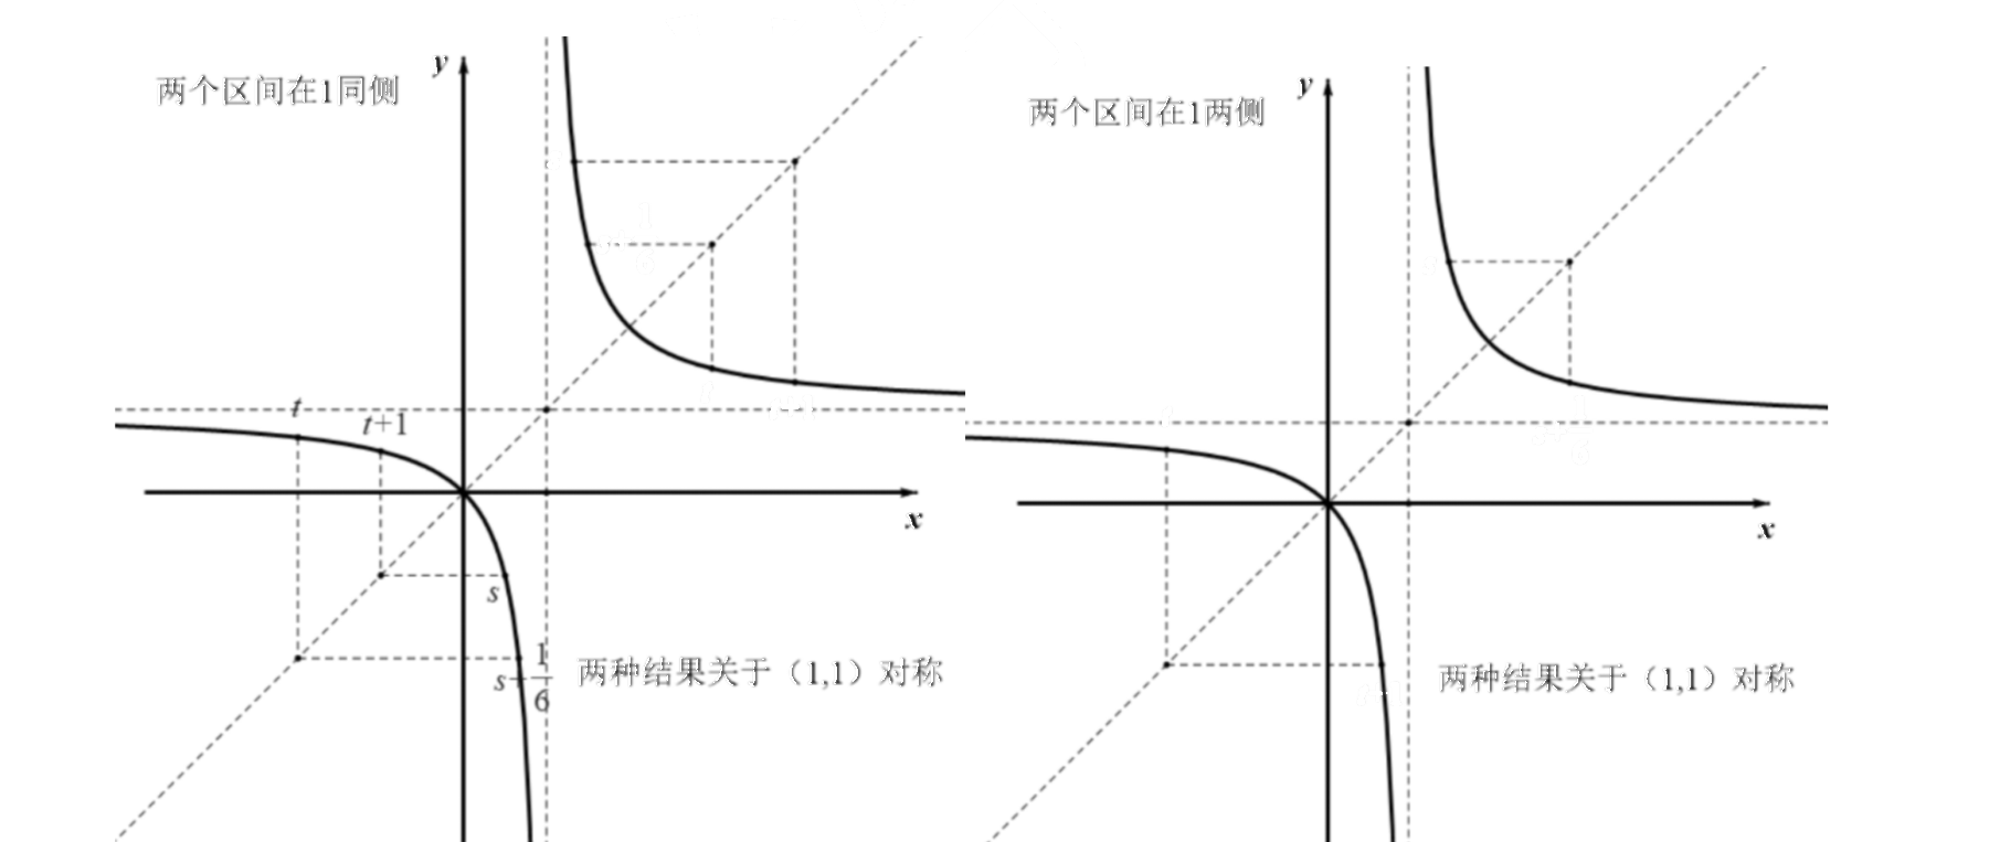
\includegraphics[width=0.92\textwidth]{figures/gao115_q10.png}
\end{center}
\solend
\fi

\end{enumerate}

\bigsec{二、选择题}

\begin{enumerate}
\setcounter{enumi}{10}

\item “对任意有理数 $x$ 都有 $x^2\neq2$”的否定形式是\mbox{（\quad）}% 原卷把答案“$B$”印在题干括号内、无【解析】

\keepwithprev
A. 存在有理数 $x$ 使得 $x^2\neq2$\qquad\qquad B. 存在有理数 $x$ 使得 $x^2=2$

C. 存在无理数 $x$ 使得 $x^2\neq2$\qquad\qquad D. 存在无理数 $x$ 使得 $x^2=2$

\ifanswer
\ans{$B$}
\fi

\item 已知 $a$、$b$ 都是实数，那么“$a^3>b^3$”是“$a^2>b^2$”的\mbox{（\quad）}

\keepwithprev
A. 充分不必要条件\qquad\qquad B. 必要不充分条件

C. 充要条件\qquad\qquad\qquad D. 既不充分也不必要条件

\ifanswer
\solbegin
\step{因为 $a^3>b^3$ 等价于 $a>b$，}
\step{由于 $a$、$b$ 正负不定，所以由 $a>b$ 不能得到 $a^2>b^2$，}
\step{由 $a^2>b^2$ 也不能得到 $a>b$，}
\step{因此“$a^3>b^3$”是“$a^2>b^2$”的既不充分也不必要条件. 故选 $D$.}
\solend
\fi

\item 定义集合运算 $A-B=\{x\mid x\in A$ 且 $x\notin B\}$，将 $A\triangle B=(A-B)\cup(B-A)$ 称为集合 $A$ 与集合 $B$ 的对称差.

命题一：$A\triangle B=B\triangle A$；

命题二：$A\triangle\varnothing=A$；

命题三：$A\cap(B\triangle C)=(A\cap B)\triangle(A\cap C)$；

命题四：$A\cup(B\triangle C)=(A\cup B)\triangle(A\cup C)$；

其中正确命题的个数是\mbox{（\quad）}

\keepwithprev
A. $1$\qquad\qquad B. $2$\qquad\qquad C. $3$\qquad\qquad D. $4$

\ifanswer
\solbegin
\step{对于①，$B\triangle A=(B-A)\cup(A-B)=(A-B)\cup(B-A)=A\triangle B$，①对；}
\step{对于②，$A-B=\{x\mid x\in A$ 且 $x\notin B\}=\{x\mid x\in A$ 且 $x\notin(A\cap B)\}$}
\step{$=A-(A\cap B)$，则 $A\triangle\varnothing=(A-\varnothing)\cup(\varnothing-A)=A\cup\varnothing=A$，②对；}
\step{对于③，$A\cap(B\triangle C)=A\cap(B\cup C-B\cap C)=A\cap(B\cup C)-A\cap(B\cap C)$}
\step{$=(A\cap B)\cup(A\cap C)-(A\cap B)\cap(A\cap C)=(A\cap B)\triangle(A\cap C)$，③对；}
\step{对于④，如图所示：}
\begin{center}
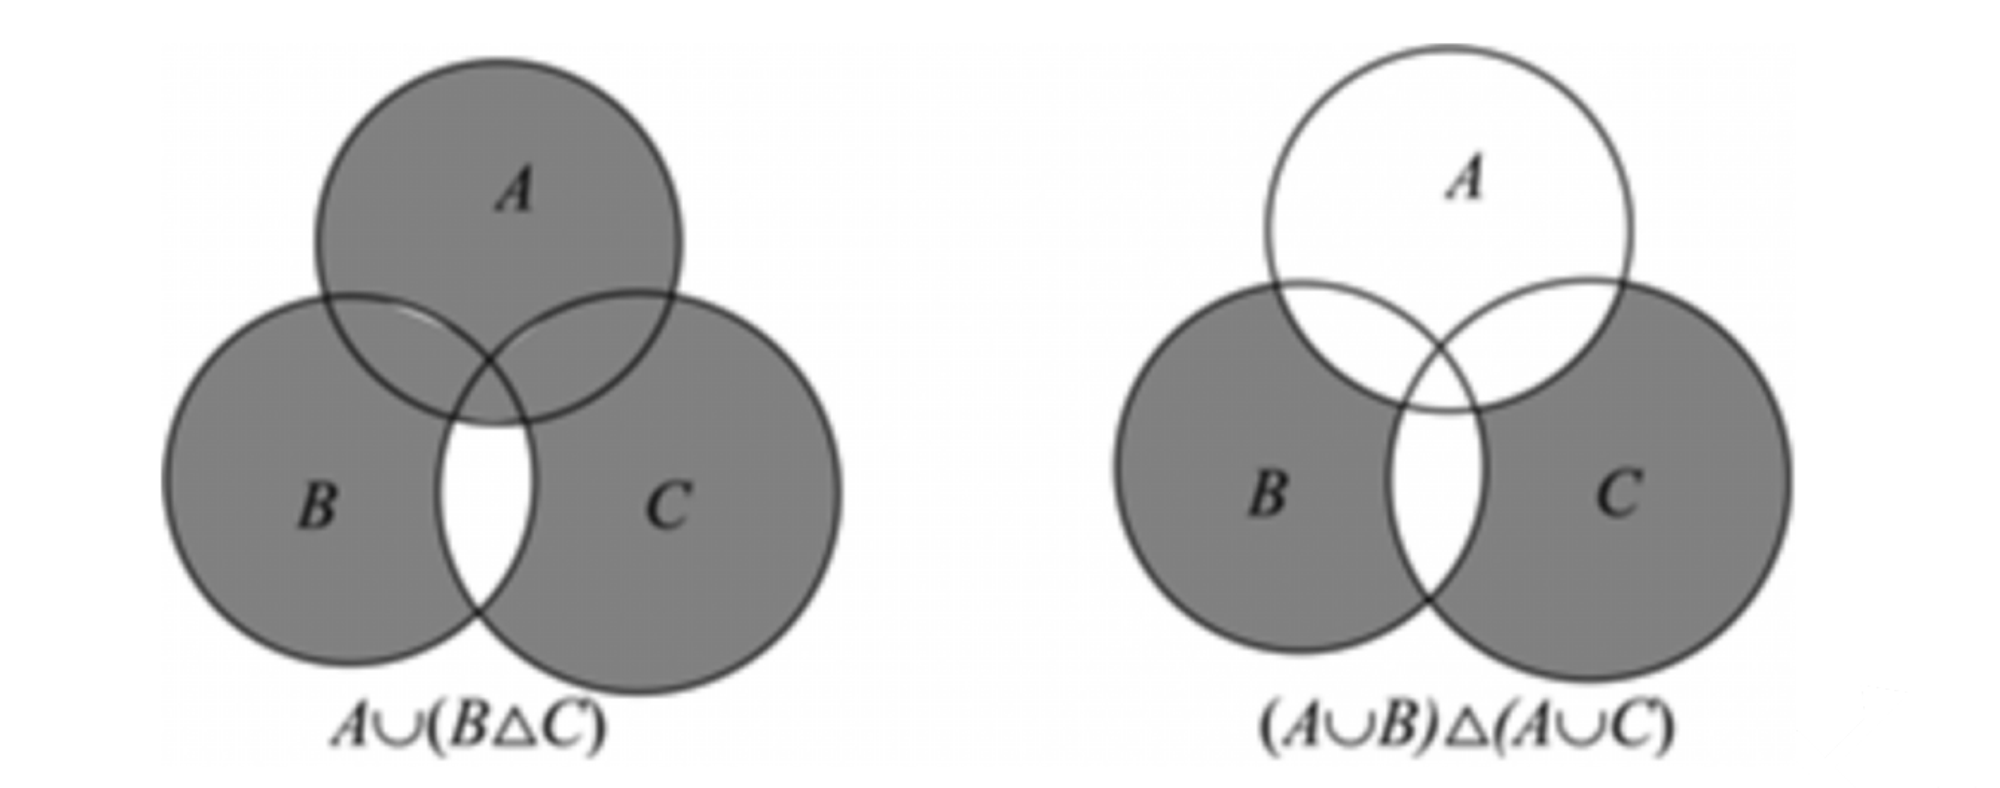
\includegraphics[width=0.85\textwidth]{figures/gao115_q13.png}
\end{center}
\step{所以 $A\cup(B\triangle C)\neq(A\cup B)\triangle(A\cup C)$，④错.}
\step{故选 $C$.}
\solend
\fi

\item 设 $a$、$b$、$c$、$p$ 为实数，若同时满足不等式 $ax^2+bx+c>0$、$bx^2+cx+a>0$ 与 $cx^2+ax+b>0$ 的全体实数 $x$ 所组成的集合等于 $(p,+\infty)$，则关于结论：① $a$、$b$、$c$ 至少有一个为 $0$；② $p=0$. 下列判断中正确的是\mbox{（\quad）}

\keepwithprev
A. ①和②都正确\qquad B. ①和②都错误\qquad C. ①正确，②错误\qquad D. ①错误，②正确

\ifanswer
\solbegin
\step{若同时满足不等式 $ax^2+bx+c>0$、$bx^2+cx+a>0$ 与 $cx^2+ax+b>0$ 的}
\step{全体实数 $x$ 所组成的集合等于 $(p,+\infty)$，必有 $a$,$b$,$c\geqslant0$，}
\step{不妨假设 $a$、$b$、$c$ 没有一个为 $0$，}
\step{则三个不等式均为开口向上的二次函数大于 $0$ 的部分，}
\step{解集的交集应为 $(-\infty,m)\cup(n,+\infty)$ 的形式，矛盾，}
\step{所以 $a$、$b$、$c$ 至少有一个为 $0$，故①正确：}
\step{不妨设 $a=0$，则 $b$,$c\geqslant0$，则不等式组化为 $\begin{cases}bx+c>0\\bx^2+cx>0,\\cx^2+b>0\end{cases}$}
\step{所以 $\begin{cases}x>-\dfrac cb\\x<-\dfrac cb\text{或}x>0\\x\in\R\end{cases}$，取交集得 $(0,+\infty)$，故 $p=0$，故②正确：}
\step{故选 $A$.}
\solend
\fi

\end{enumerate}

\bigsec{三、解答题}

\begin{enumerate}
\setcounter{enumi}{14}

\item 已知 $a>0$，$b>0$，

（1）试比较 $\dfrac{a^2-b^2}{a^2+b^2}$ 与 $\dfrac{a-b}{a+b}$ 的大小；

（2）若 $a+b>4$，求证：$\dfrac a{b+2}$ 和 $\dfrac b{a+2}$ 中至少有一个大于 $\dfrac12$.

\ifanswer
\solbegin
\step{（1）已知 $a>0$，$b>0$，$\dfrac{a^2-b^2}{a^2+b^2}-\dfrac{a-b}{a+b}=\dfrac{2ab(a-b)}{(a^2+b^2)(a+b)}$，}
\step{当 $a>b$ 时，$a-b>0$，所以 $\dfrac{a^2-b^2}{a^2+b^2}-\dfrac{a-b}{a+b}>0$，所以 $\dfrac{a^2-b^2}{a^2+b^2}>\dfrac{a-b}{a+b}$；}
\step{当 $a=b$ 时，$a-b=0$，所以 $\dfrac{a^2-b^2}{a^2+b^2}-\dfrac{a-b}{a+b}=0$，所以 $\dfrac{a^2-b^2}{a^2+b^2}=\dfrac{a-b}{a+b}$；}
\step{当 $a<b$ 时，$a-b<0$，所以 $\dfrac{a^2-b^2}{a^2+b^2}-\dfrac{a-b}{a+b}<0$，所以 $\dfrac{a^2-b^2}{a^2+b^2}<\dfrac{a-b}{a+b}$；}
\step{（2）假设 $\dfrac a{b+2}$ 和 $\dfrac b{a+2}$ 中都不大于 $\dfrac12$，即 $\dfrac b{a+2}\leqslant\dfrac12$，$\dfrac a{b+2}\leqslant\dfrac12$，}
\step{因为 $a>0$，$b>0$，所以 $a+2>0$，$b+2>0$，}
\step{所以 $2b\leqslant a+2$，$2a\leqslant b+2$，}
\step{两式相加得 $2a+2b\leqslant a+2+b+2=a+b+4$，即 $a+b\leqslant4$，}
\step{与已知 $a+b>4$ 矛盾，所以假设错误，}
\step{故 $\dfrac a{b+2}$ 和 $\dfrac b{a+2}$ 中至少有一个大于 $\dfrac12$.}
\solend
\fi

\item 某企业原有 $200$ 名科技人员，年人均工资 $a$ 万元($a>0$). 现加大对某芯片研发力度，该企业把原有 $200$ 名科技人员调整成技术人员和研发人员，其中技术人员 $x$ 名($x\in\N$ 且 $40\leqslant x\leqslant80$). 调整后，研发人员的年人均工资比调整前增加了 $(2x)\%$，技术人员的年人均工资为 $a\left(m-\dfrac x{10}\right)$万元.

（1）若要使调整后研发人员的年总工资不低于调整前 $200$ 名科技人员年总工资的 $1.5$ 倍，求调整后的技术人员最少有多少人？

（2）为了激励研发人员的工作热情和保持技术人员的工作积极性，企业决定在工资方面要同时满足以下两个条件：

①研发人员的年总工资始终不低于技术人员的年总工资；

②技术人员的年人均工资始终不低于调整前 $200$ 名科技人员的年人均工资.

请问是否存在这样的实数 $m$？若存在，求出 $m$ 的范围；若不存在，说明理由.

\ifanswer
\solbegin
\step{（1）由题意得调整后研发人员的年人均工资为 $[1+(2x)\%]a$ 万元，}
\step{那么 $(200-x)[1+(2x)\%]a\geqslant1.5\times200a$ ($a>0$)，}
\step{化简得 $x^2-150x+5000\leqslant0$，解得 $50\leqslant x\leqslant100$，}
\step{由于 $x\in\N$ 且 $40\leqslant x\leqslant80$，因此 $50\leqslant x\leqslant80$，}
\step{因此调整后的技术人员的人数最少为 $50$ 人；}
\step{（2）假设存在实数 $m$，使得技术人员在已知范围内调整后，满足以上两个条件，}
\step{由条件①得 $(200-x)[1+(2x)\%]a\geqslant x\left(m-\dfrac x{10}\right)a$，}
\step{整理得 $m\leqslant\dfrac{200}{x}+\dfrac{2x}{25}+3$；}
\step{因为 $\dfrac{200}{x}+\dfrac{2x}{25}+3\geqslant2\sqrt{\dfrac{200}{x}\cdot\dfrac{2x}{25}}+3=11$，}
\step{当且仅当 $\dfrac{200}{x}=\dfrac{2x}{25}$，即 $x=50$ 时取等号，因此 $m\leqslant11$，}
\step{由条件②得 $a\left(m-\dfrac x{10}\right)\geqslant a$，所以 $m\geqslant\dfrac x{10}+1$；}
\step{又由于 $40\leqslant x\leqslant80$，因此 $m\geqslant9$.}
\step{因此 $m\in[9,11]$.}
\solend
\fi

\item 已知 $a\in\R$，记 $f(x)=ax^2-(a+2)x+2$.

（1）若 $f(x)<3-2x$ 对于一切 $x\in\R$ 恒成立，求实数 $a$ 的取值范围；

（2）求关于 $x$ 不等式 $f(x)\geqslant0$ 的解集；

（3）若存在 $m\in\R$ 使关于 $x$ 的方程 $ax^2-(a+2)\lvert x\rvert+2=\lvert m+2\rvert+\lvert m-1\rvert$ 有四个不同的实根，求实数 $a$ 的取值范围.

\ifanswer
\solbegin
\step{（1）由 $f(x)<3-2x$ 对于一切 $x\in\R$ 恒成立，}
\step{得 $ax^2-ax-1<0$ 对于一切 $x\in\R$ 恒成立，}
\step{当 $a=0$ 时，原式可化为 $-1<0$，恒成立，符合条件；}
\step{当 $a\neq0$ 时，需满足 $\begin{cases}a<0\\\Delta=a^2+4a<0\end{cases}$，解得 $-4<a<0$；}
\step{综上，实数 $a$ 的取值范围是 $(-4,0]$；}
\step{（2）$f(x)\geqslant0$，即 $(ax-2)(x-1)\geqslant0$，}
\step{当 $a=0$ 时，原式化为 $-2x+2\geqslant0$，解集为 $\{x\mid x\leqslant1\}$；}
\step{当 $a>0$ 时，若 $a=2$，原式化为 $2(x-1)^2\geqslant0$，解集为 $\R$；}
\step{若 $0<a<2$，$\dfrac2a>1$，解集为 $\{x\mid x\leqslant1$ 或 $x\geqslant\dfrac2a\}$；}
\step{若 $a>2$，$\dfrac2a<1$，解集为 $\{x\mid x\leqslant\dfrac2a$ 或 $x\geqslant1\}$；}
\step{当 $a<0$ 时，$\dfrac2a<1$，解集为 $\left\{x\,\middle\vert\,\dfrac2a\leqslant x\leqslant1\right\}$；}
\step{综上，当 $a<0$ 时，不等式解集为 $\left\{x\,\middle\vert\,\dfrac2a\leqslant x\leqslant1\right\}$；}
\step{当 $a=0$ 时，不等式解集为 $\{x\mid x\leqslant1\}$；}
\step{当 $0<a<2$ 时，不等式解集为 $\{x\mid x\leqslant1$ 或 $x\geqslant\dfrac2a\}$；}
\step{当 $a=2$ 时，不等式解集为 $\R$；}
\step{当 $a>2$ 时，不等式解集为 $\{x\mid x\leqslant\dfrac2a$ 或 $x\geqslant1\}$；}
\step{（3）由绝对值三角不等式得 $\lvert m+2\rvert+\lvert m-1\rvert\geqslant\lvert(m+2)-(m-1)\rvert=3$，}
\step{即右侧取值范围为 $[3,+\infty)$，}
\step{令 $t=\lvert x\rvert\geqslant0$，原方程转化为 $at^2-(a+2)t+2=k$，$k\in[3,+\infty)$，}
\step{若原方程有四个不同实根，}
\step{需存在 $k\geqslant3$，使得方程 $at^2-(a+2)t+2-k=0$ 有两个不同正实根，}
\step{当 $a\geqslant0$ 时，方程的两根之积为 $\dfrac{2-k}{a}$，}
\step{因为 $k\geqslant3$，所以 $2-k\leqslant-1<0$，两根一正一负，}
\step{最多只有一个正根，对应最多两个 $x$ 根，不符合要求；}
\step{当 $a<0$ 时，两根之积为正，}
\step{要两个根都为正，需要两根之和 $\dfrac{a+2}{a}>0$，解得 $a<-2$，}
\step{再要求存在 $k\geqslant3$ 使得判别式大于 $0$，}
\step{即 $\triangle=(a+2)^2-4a(2-k)>0$ 在 $k\in[3,+\infty)$ 上有解，}
\step{即 $(a-2)^2+4ak>0$ 在 $k\in[3,+\infty)$ 上有解，}
\step{由 $a<0$，得 $(a-2)^2+12a>0$，}
\step{即 $a^2+8a+4>0$，结合 $a<-2$ 解得 $a<-4-2\sqrt3$，}
\step{故实数 $a$ 的取值范围是 $(-\infty,-4-2\sqrt3)$.}
\solend
\fi

\item 设 $A=\{x_1,x_2,\cdots,x_n\}(n\geqslant2,n\in\N)$，且 $x_1,x_2,\cdots,x_n$ 均为正整数，若对于 $A$ 中任意两个元素 $a,b$，当 $a>b$ 时，都有 $\dfrac{b^2}{a-b}\in A$，则称 $A$ 为“$n$ 元好集”.

（1）判断 $\{2,4,6\}$ 是否为“三元好集”，并说明理由；

（2）若集合 $M$ 为“二元好集”，且 $M$ 中所有元素之积小于 $2026$，求所有满足条件的集合 $M$ 的个数；

（3）设 $k\geqslant3,k\in\N$，是否存在“$k$ 元好集”，若存在，求出所有满足条件的“$k$ 元好集”，若不存在，请说明理由.

\ifanswer
\solbegin
\step{（1）取 $a=6,b=2$，则 $\dfrac{b^2}{a-b}=\dfrac44=1\notin\{2,4,6\}$，所以该集合不是三元好集.}
\step{（2）设 $M=\{b,a\}$，其中 $a>b$ 且均为正整数，则 $\dfrac{b^2}{a-b}$ 等于 $a$ 或 $b$.}
\step{若 $\dfrac{b^2}{a-b}=a$，则 $a^2-ab-b^2=0$，从而 $\dfrac ab=\dfrac{1+\sqrt5}{2}$，与 $\dfrac ab$ 为有理数矛盾.}
\step{若 $\dfrac{b^2}{a-b}=b$，则 $a=2b$；}
\step{反之，任意正整数 $b$ 对应的 $\{b,2b\}$ 均为二元好集.}
\step{由元素之积小于 $2026$，得 $2b^2<2026\Leftrightarrow b^2<1013$.}
\step{因为 $31^2=961<1013<1024=32^2$，所以 $b=1,2,\cdots,31$，}
\step{对应 $31$ 个不同的集合.}
\step{（3）假设存在 $k\geqslant3$ 的 $k$ 元好集 $A$，将其元素从小到大排列，}
\step{记最小元素为 $u$，次小元素为 $v$，最大元素为 $w$，则 $0<u<v<w$.}
\step{由 $\dfrac{u^2}{w-u}\in A$，该数不小于 $u$，得 $\dfrac{u^2}{w-u}\geqslant u\Rightarrow w\leqslant2u$.}
\step{又由 $\dfrac{u^2}{v-u}$,$\dfrac{v^2}{w-v}\in A$，这两个数均不超过 $w$，}
\step{得 $\dfrac{u^2}{v-u}\leqslant w$,$\dfrac{v^2}{w-v}\leqslant w$，}
\step{分母均为正，分别去分母后相加，}
\step{得 $u^2+v^2\leqslant w(v-u)+w(w-v)=w(w-u)\leqslant2u^2$，}
\step{于是 $v^2\leqslant u^2$，与 $v>u>0$ 矛盾，所以不存在 $k\geqslant3$ 的 $k$ 元好集.}
\solend
\fi

\end{enumerate}

\end{document}
"
% 紧凑版：xelatex "\def\iscompact{1}% 高一115_复旦附中_10月阶段练习.tex
%   —— 高一上数学“2026-2027 年复旦附中高一上 10 月阶段练习”（试卷版/答案版）
% 试卷版：xelatex 高一115_复旦附中_10月阶段练习.tex
% 答案版：xelatex "\def\isanswer{1}\input{高一115_复旦附中_10月阶段练习.tex}"
% 紧凑版：xelatex "\def\iscompact{1}\input{高一115_复旦附中_10月阶段练习.tex}"
%
% 原始材料：微信公众号“魔都数学加油站”文章，作者破晓，2026-11-06 17:58 发布；
% 连载“27学年高一115”，原文标题“27学年高一115——2026-2027年上海市复旦附中高一上10月阶段练习”；
% 原文链接：https://mp.weixin.qq.com/s/krocP0fMQQ4VM1SQEcLI2Q。
% 正文为 12 张 PNG 页（第 4、6、12 页 2560×3620，其余 4762×6735），
% 题目下印有【解析】或【答案】，为讲评版。
% 题目、解析均据原图转录；卷面红色水印及公众号页脚未录入。
%
% 卷首标题：原卷印作“2026-2027 年复旦附中高一上 10 月阶段练习”（公众号标题中的“上海市”
% 卷面标题行没有，本稿照卷面），年份区间按全稿惯例排 en dash；原卷未印副标题，本稿按题目内容
% 标为“集合与常用逻辑用语、不等式”。
%
% 与原卷的排版差异：
%   ① 原文从第 3 题起，填空题编号为 3—10、选择题为 11—14、解答题为 15—18，共 16 题，
%      本稿保留原题号（与多数卷的 3—21 不同）；
%   ② 原卷每题下直接印【解析】／【答案】，本稿按全稿惯例置于答案版；第 11 题把答案“$B$”
%      印在题干括号内且无【解析】，另提 \ans{}；其余选择题答案在解析末句“故选 …”，括号内留空；
%   ③ 原卷未印副标题，本稿按“知识模块”口径补出；
%   ④ 原卷填空横线按全稿惯例排为 \blankline[4.4em]；选择题括号排 \mbox{（\quad）}、
%      选项段前按惯例加 \keepwithprev；解答题不留作答区（原卷为讲评版，与 109—114 同）；
%   ⑤ 原卷数集排斜体 $R$／$Q$／$N$，按全稿惯例改 \R、\Q、\N。
%
% 判别式与对称差字形：原卷 $\triangle$（等边、扁）与 $\Delta$（等腰、高）两种混用，逐处照录——
%   第 7 题与第 17 题 (3) 的判别式、第 13 题的对称差 $A\triangle B$ 用 \triangle，
%   第 17 题 (1) cases 的判别式用 \Delta。
%
% 子集符号：第 4 题解析的 $(-1,3)\subset(-m,m)$ 印单线（真子集、无下划线），按 18／96
%   成例照录 \subset；第 5 题解析的 $B\subseteq A$ 印有下划线，照录 \subseteq。
%   第 3 题的补集照原卷上划线排 \overline{N}。
%
% 原卷存疑照录：第 9 题解析末行“故可能成立的是①②③”与四种情形的编号一致，照录；
%   第 10 题解析两幅函数图上另有蓝色／红色手写标注（$t$、$t+1$、$s$、$\frac16$ 等），
%   系批改笔迹，随裁图保留、不另作正文录入；第 14 题解析的 cases 三行照原卷排；
%   第 18 题 (2) 解析“所以该集合不是三元好集”前的取例 $a=6,b=2$ 照录。
%
% 行数核对：逐题数 \step/\stepm 条数，合计 133 条（Q3：3；Q4：3；Q5：4；Q6：5；Q7：4；
% Q8：4；Q9：11；Q10：7；Q11：0；Q12：4；Q13：8；Q14：9；Q15：10；Q16：13；
% Q17：32；Q18：16），与原卷印刷行逐题相等（cases 块作一个印刷行计）。第 11 题括号内印
% 答案且无解析，提 \ans{}，不计入 \step 账；第 10、13 题解析内的插图不计入 \step 账。
%
\documentclass[a4paper,11pt]{article}
\usepackage{common}

\begin{document}

\examtitlest[3]{2026--2027 年复旦附中高一上 10 月阶段练习}{集合与常用逻辑用语、不等式}

\bigsec{一、填空题}

\begin{enumerate}
\setcounter{enumi}{2}

\item 已知集合 $M=\{x\mid 4x^2-4x-15>0\}$，$N=\left\{x\,\middle\vert\,\dfrac{x+1}{x-6}>0\right\}$，则 $M\cap\overline{N}=$\blankline[4.4em].

\ifanswer
\solbegin
\step{集合 $M=\{x\mid 4x^2-4x-15>0\}=\{x\mid x>\dfrac52$ 或 $x<-\dfrac32\}$，}
\step{$N=\left\{x\,\middle\vert\,\dfrac{x+1}{x-6}>0\right\}=\{x\mid x>6$ 或 $x<-1\}$，得 $\overline{N}=\{x\mid-1\leqslant x\leqslant6\}$，}
\step{故 $M\cap\overline{N}=\left\{x\,\middle\vert\,\dfrac52<x\leqslant6\right\}$.}
\solend
\fi

\item 已知 $m>0$，不等式 $\lvert x\rvert<m$ 成立的一个充分不必要条件是 $-1<x<3$，则 $m$ 的取值范围是\blankline[4.4em].

\ifanswer
\solbegin
\step{不等式 $-m<x<m$ 成立的一个充分不必要条件是 $-1<x<3$，}
\step{由题意得 $(-1,3)\subset(-m,m)$，则 $m\geqslant3$，此时 $-m\leqslant-3<-1$，}% 原卷印单线 \subset，照录
\step{所以 $m$ 的取值范围是 $\{m\mid m\geqslant3\}$.}
\solend
\fi

\item 已知集合 $A=\{1,2\}$，集合 $B=\{x\mid ax=6\}$，若 $A\cup B=A$，则 $a$ 的所有取值构成的集合为\blankline[4.4em].

\ifanswer
\solbegin
\step{因为 $A\cup B=A$，所以 $B\subseteq A$，}
\step{当 $a=0$ 时，$B=\varnothing$，满足 $B\subseteq A$；}
\step{当 $a\neq0$ 时，$B=\left\{\dfrac6a\right\}$，则 $\dfrac6a=1$ 或 $\dfrac6a=2$，解得 $a=6$ 或 $a=3$，}
\step{综上所述，$a$ 的所有取值构成的集合为 $\{0,3,6\}$.}
\solend
\fi

\item 若关于 $x$ 的不等式 $ax^2+bx+c>0$ 的解集为 $(-3,2)$，则不等式 $ax^2+(a+b)x+c-2a>0$ 的解集为\blankline[4.4em].

\ifanswer
\solbegin
\step{由 $ax^2+bx+c>0$ 的解集为 $(-3,2)$ 得 $a<0$，}
\step{且 $ax^2+bx+c=0$ 时 $x_1=-3$，$x_2=2$，}
\step{得 $-3+2=-\dfrac ba$，即 $b=a$，$-3\times2=\dfrac ca$，即 $c=-6a$，}
\step{代入 $ax^2+(a+b)x+c-2a>0$ 得 $ax^2+2ax-8a>0$ 化简得 $x^2+2x-8<0$，}
\step{解得 $-4<x<2$，故解集为 $(-4,2)$.}
\solend
\fi

\item 已知关于 $x$ 的方程 $x^2-2x+m=0$ 的两个实数根分别为 $x_1$，$x_2$. 若 $x_1^2x_2^2+x_1^2+x_2^2=7$，则实数 $m$ 的值为\blankline[4.4em].

\ifanswer
\solbegin
\step{由韦达定理得 $x_1+x_2=2$，$x_1x_2=m$，}
\step{$x_1^2x_2^2+x_1^2+x_2^2=(x_1x_2)^2+(x_1+x_2)^2-2x_1x_2=m^2+4-2m$，}
\step{由 $m^2+4-2m=7$，得 $m^2-2m-3=0$，解得 $m=3$ 或 $m=-1$，}
\step{方程有两个实数根，故 $\triangle=4-4m\geqslant0$，即 $m\leqslant1$，所以 $m=-1$.}
\solend
\fi

\item 已知 $x>1$，若 $x^2-xy+y=0$，则 $x+y$ 的最小值是\blankline[4.4em].

\ifanswer
\solbegin
\step{由于 $x^2-xy+y=0$，则 $y=\dfrac{x^2}{x-1}>0$，}
\step{则 $x+y=x+\dfrac{x^2}{x-1}=\dfrac{2x^2-x}{x-1}=\dfrac{2(x-1)^2+3(x-1)+1}{x-1}$}
\step{$=2(x-1)+\dfrac1{x-1}+3\geqslant2\sqrt{2(x-1)\cdot\dfrac1{x-1}}+3=2\sqrt2+3$，}
\step{当且仅当 $x=1+\dfrac{\sqrt2}{2}$ 时取等号，故最小值是 $2\sqrt2+3$.}
\solend
\fi

\item 若集合 $A=B_1\cup B_2\cup\cdots\cup B_n$，其中 $B_1$、$B_2$、$\cdots$、$B_n$ 为非空集合，$B_i\cap B_j=\varnothing$，$1\leqslant i<j\leqslant n$，则称集合 $\{B_1,B_2,\cdots,B_n\}$ 为集合 $A$ 的一个 $n$ 划分. 例如：集合 $\{\{1,2\},\{3\}\}$，$\{\{1,3\},\{2\}\}$，$\{\{2,3\},\{1\}\}$ 均为集合 $\{1,2,3\}$ 的一个 $2$ 划分. 设 $\{B_1,B_2\}$ 为有理数集 $\Q$ 的一个 $2$ 划分，且满足对任意 $x\in B_1$，任意 $y\in B_2$，都有 $x<y$. 则对于 $B_1$、$B_2$ 有：

① $B_1$ 中的元素存在最大值，$B_2$ 中的元素不存在最小值；

② $B_1$ 中的元素不存在最大值，$B_2$ 中的元素存在最小值；

③ $B_1$ 中的元素不存在最大值，$B_2$ 中的元素不存在最小值；

④ $B_1$ 中的元素存在最大值，$B_2$ 中的元素存在最小值；

对于以上四种情况，可能成立的序号有\blankline[4.4em].

\ifanswer
\solbegin
\step{对于①，$B_1=\{x\in\Q\mid x\leqslant2\}$，$B_2=\{x\in\Q\mid x>2\}$，①可能成立；}
\step{对于②，$B_1=\{x\in\Q\mid x<2\}$，$B_2=\{x\in\Q\mid x\geqslant2\}$，②可能成立；}
\step{对于③，$B_1=\{x\in\Q\mid x<\pi\}$，$B_2=\{x\in\Q\mid x>\pi\}$，③可能成立；}
\step{对于④，假设④成立，}
\step{不妨设 $B_1$ 中的元素的最大值为 $s$，$B_2$ 中的元素的最小值为 $t$，}
\step{由题意得 $s<t$，所以 $s<\dfrac{s+t}{2}<t$，}
\step{因为 $s$ 为 $B_1$ 中的元素的最大值，所以 $\dfrac{s+t}{2}\notin B_1$，}
\step{因为 $t$ 为 $B_2$ 中的元素的最小值，所以 $\dfrac{s+t}{2}\notin B_2$，}
\step{又 $B_1\cup B_2=\Q$，所以 $\dfrac{s+t}{2}\notin\Q$，与 $\dfrac{s+t}{2}\in\Q$ 矛盾，}
\step{所以假设不成立，即④不可能成立.}
\step{故可能成立的是①②③.}
\solend
\fi

\item 已知集合 $A=\left[s,s+\dfrac16\right]\cup[t,t+1]$，其中 $1\notin A$ 且 $s+\dfrac16<t$，函数 $f(x)=\dfrac x{x-1}$，且对任意 $a\in A$，都有 $f(a)\in A$，则 $t$ 的值是\blankline[4.4em].

\ifanswer
\solbegin
\step{若 $\left[s,s+\dfrac16\right]$,$[t,t+1]$ 在 $f(x)=\dfrac x{x-1}$ 图像的同侧，}
\step{则点 $\left(t,s+\dfrac16\right)$,$(t+1,s)$ 在 $f(x)=\dfrac x{x-1}$ 的图像上，}
\step{所以 $\dfrac t{t-1}=\dfrac{t+1}{t}+\dfrac16$，解得 $t=-2$ 或 $t=3$，检验得 $t=3$；}
\step{若 $\left[s,s+\dfrac16\right]$,$[t,t+1]$ 在 $f(x)=\dfrac x{x-1}$ 图像的两侧，}
\step{则点 $(t,t+1)$ 在 $f(x)=\dfrac x{x-1}$ 的图像上，}
\step{所以 $t+1=\dfrac t{t-1}$，解得 $t=\dfrac{1\pm\sqrt5}{2}$，检验得 $t=\dfrac{1+\sqrt5}{2}$，}
\step{综上，$t=\dfrac{1+\sqrt5}{2}$ 或 $t=3$.}
\begin{center}
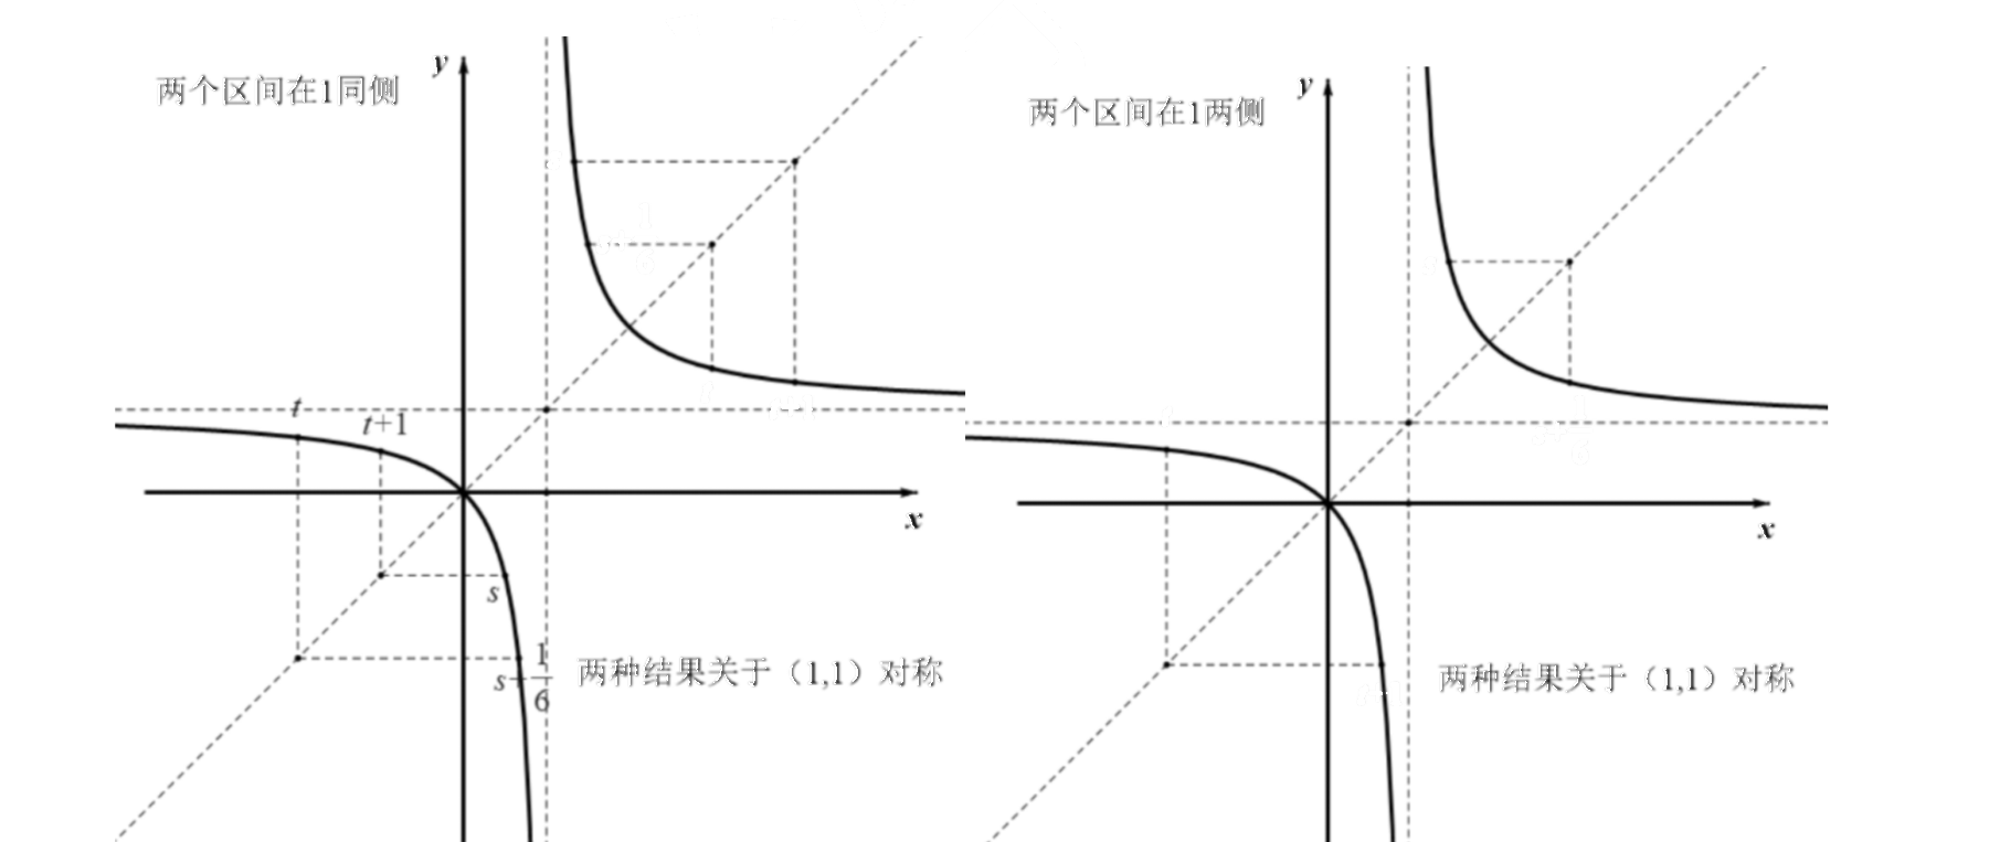
\includegraphics[width=0.92\textwidth]{figures/gao115_q10.png}
\end{center}
\solend
\fi

\end{enumerate}

\bigsec{二、选择题}

\begin{enumerate}
\setcounter{enumi}{10}

\item “对任意有理数 $x$ 都有 $x^2\neq2$”的否定形式是\mbox{（\quad）}% 原卷把答案“$B$”印在题干括号内、无【解析】

\keepwithprev
A. 存在有理数 $x$ 使得 $x^2\neq2$\qquad\qquad B. 存在有理数 $x$ 使得 $x^2=2$

C. 存在无理数 $x$ 使得 $x^2\neq2$\qquad\qquad D. 存在无理数 $x$ 使得 $x^2=2$

\ifanswer
\ans{$B$}
\fi

\item 已知 $a$、$b$ 都是实数，那么“$a^3>b^3$”是“$a^2>b^2$”的\mbox{（\quad）}

\keepwithprev
A. 充分不必要条件\qquad\qquad B. 必要不充分条件

C. 充要条件\qquad\qquad\qquad D. 既不充分也不必要条件

\ifanswer
\solbegin
\step{因为 $a^3>b^3$ 等价于 $a>b$，}
\step{由于 $a$、$b$ 正负不定，所以由 $a>b$ 不能得到 $a^2>b^2$，}
\step{由 $a^2>b^2$ 也不能得到 $a>b$，}
\step{因此“$a^3>b^3$”是“$a^2>b^2$”的既不充分也不必要条件. 故选 $D$.}
\solend
\fi

\item 定义集合运算 $A-B=\{x\mid x\in A$ 且 $x\notin B\}$，将 $A\triangle B=(A-B)\cup(B-A)$ 称为集合 $A$ 与集合 $B$ 的对称差.

命题一：$A\triangle B=B\triangle A$；

命题二：$A\triangle\varnothing=A$；

命题三：$A\cap(B\triangle C)=(A\cap B)\triangle(A\cap C)$；

命题四：$A\cup(B\triangle C)=(A\cup B)\triangle(A\cup C)$；

其中正确命题的个数是\mbox{（\quad）}

\keepwithprev
A. $1$\qquad\qquad B. $2$\qquad\qquad C. $3$\qquad\qquad D. $4$

\ifanswer
\solbegin
\step{对于①，$B\triangle A=(B-A)\cup(A-B)=(A-B)\cup(B-A)=A\triangle B$，①对；}
\step{对于②，$A-B=\{x\mid x\in A$ 且 $x\notin B\}=\{x\mid x\in A$ 且 $x\notin(A\cap B)\}$}
\step{$=A-(A\cap B)$，则 $A\triangle\varnothing=(A-\varnothing)\cup(\varnothing-A)=A\cup\varnothing=A$，②对；}
\step{对于③，$A\cap(B\triangle C)=A\cap(B\cup C-B\cap C)=A\cap(B\cup C)-A\cap(B\cap C)$}
\step{$=(A\cap B)\cup(A\cap C)-(A\cap B)\cap(A\cap C)=(A\cap B)\triangle(A\cap C)$，③对；}
\step{对于④，如图所示：}
\begin{center}
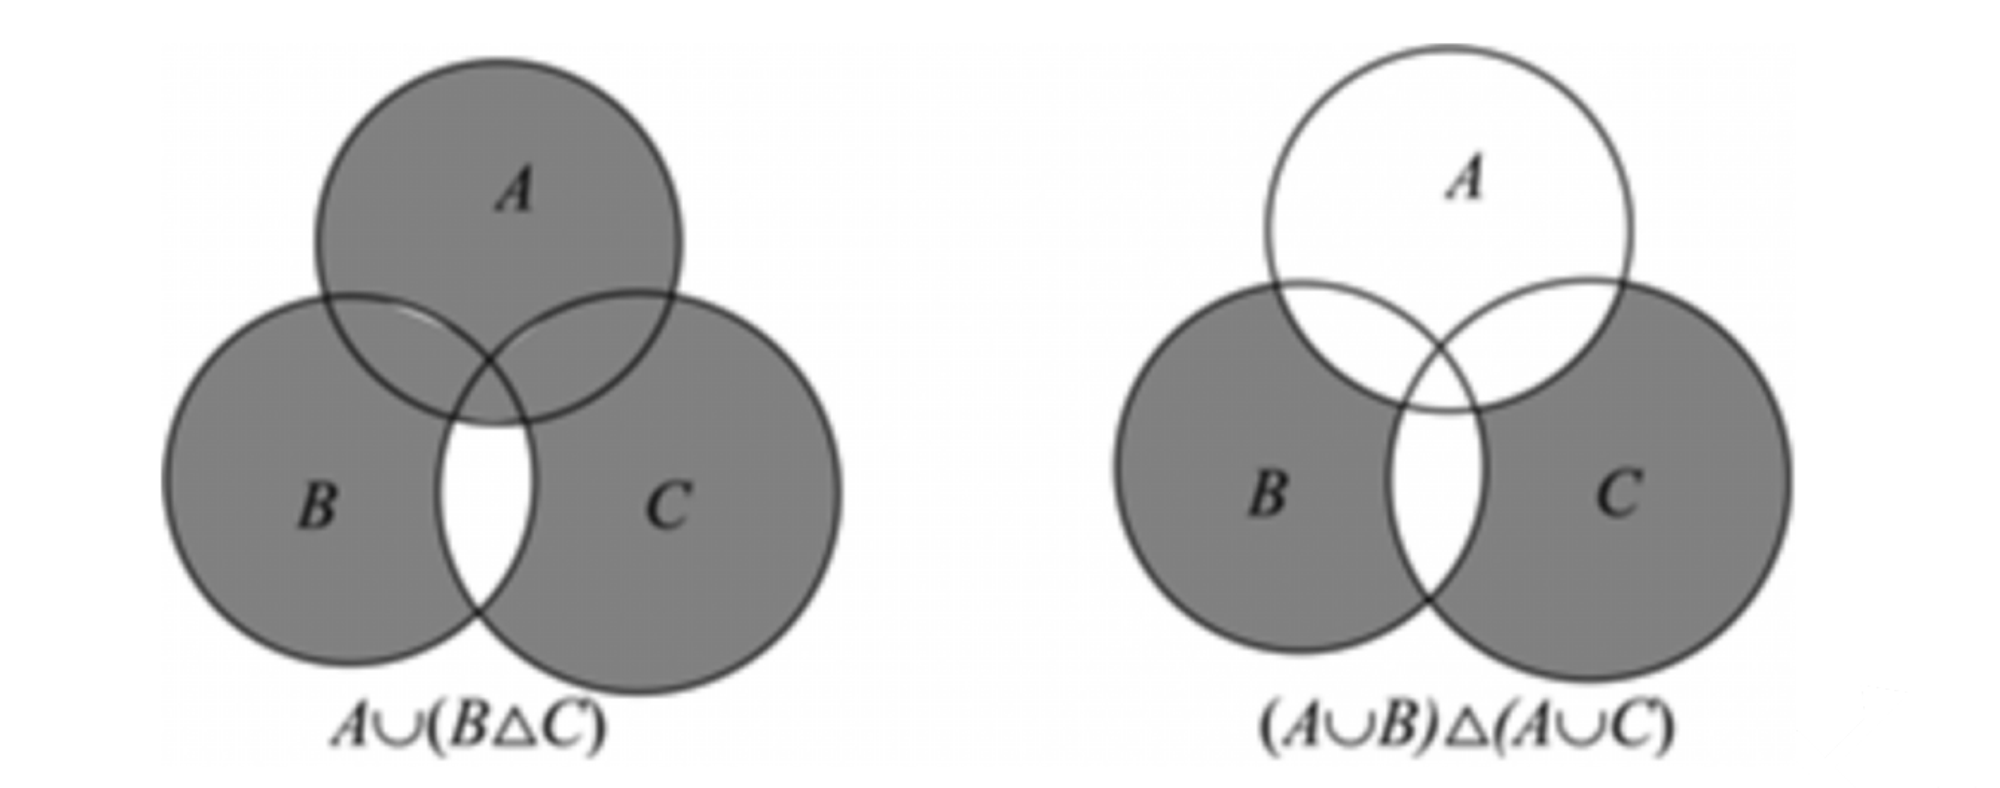
\includegraphics[width=0.85\textwidth]{figures/gao115_q13.png}
\end{center}
\step{所以 $A\cup(B\triangle C)\neq(A\cup B)\triangle(A\cup C)$，④错.}
\step{故选 $C$.}
\solend
\fi

\item 设 $a$、$b$、$c$、$p$ 为实数，若同时满足不等式 $ax^2+bx+c>0$、$bx^2+cx+a>0$ 与 $cx^2+ax+b>0$ 的全体实数 $x$ 所组成的集合等于 $(p,+\infty)$，则关于结论：① $a$、$b$、$c$ 至少有一个为 $0$；② $p=0$. 下列判断中正确的是\mbox{（\quad）}

\keepwithprev
A. ①和②都正确\qquad B. ①和②都错误\qquad C. ①正确，②错误\qquad D. ①错误，②正确

\ifanswer
\solbegin
\step{若同时满足不等式 $ax^2+bx+c>0$、$bx^2+cx+a>0$ 与 $cx^2+ax+b>0$ 的}
\step{全体实数 $x$ 所组成的集合等于 $(p,+\infty)$，必有 $a$,$b$,$c\geqslant0$，}
\step{不妨假设 $a$、$b$、$c$ 没有一个为 $0$，}
\step{则三个不等式均为开口向上的二次函数大于 $0$ 的部分，}
\step{解集的交集应为 $(-\infty,m)\cup(n,+\infty)$ 的形式，矛盾，}
\step{所以 $a$、$b$、$c$ 至少有一个为 $0$，故①正确：}
\step{不妨设 $a=0$，则 $b$,$c\geqslant0$，则不等式组化为 $\begin{cases}bx+c>0\\bx^2+cx>0,\\cx^2+b>0\end{cases}$}
\step{所以 $\begin{cases}x>-\dfrac cb\\x<-\dfrac cb\text{或}x>0\\x\in\R\end{cases}$，取交集得 $(0,+\infty)$，故 $p=0$，故②正确：}
\step{故选 $A$.}
\solend
\fi

\end{enumerate}

\bigsec{三、解答题}

\begin{enumerate}
\setcounter{enumi}{14}

\item 已知 $a>0$，$b>0$，

（1）试比较 $\dfrac{a^2-b^2}{a^2+b^2}$ 与 $\dfrac{a-b}{a+b}$ 的大小；

（2）若 $a+b>4$，求证：$\dfrac a{b+2}$ 和 $\dfrac b{a+2}$ 中至少有一个大于 $\dfrac12$.

\ifanswer
\solbegin
\step{（1）已知 $a>0$，$b>0$，$\dfrac{a^2-b^2}{a^2+b^2}-\dfrac{a-b}{a+b}=\dfrac{2ab(a-b)}{(a^2+b^2)(a+b)}$，}
\step{当 $a>b$ 时，$a-b>0$，所以 $\dfrac{a^2-b^2}{a^2+b^2}-\dfrac{a-b}{a+b}>0$，所以 $\dfrac{a^2-b^2}{a^2+b^2}>\dfrac{a-b}{a+b}$；}
\step{当 $a=b$ 时，$a-b=0$，所以 $\dfrac{a^2-b^2}{a^2+b^2}-\dfrac{a-b}{a+b}=0$，所以 $\dfrac{a^2-b^2}{a^2+b^2}=\dfrac{a-b}{a+b}$；}
\step{当 $a<b$ 时，$a-b<0$，所以 $\dfrac{a^2-b^2}{a^2+b^2}-\dfrac{a-b}{a+b}<0$，所以 $\dfrac{a^2-b^2}{a^2+b^2}<\dfrac{a-b}{a+b}$；}
\step{（2）假设 $\dfrac a{b+2}$ 和 $\dfrac b{a+2}$ 中都不大于 $\dfrac12$，即 $\dfrac b{a+2}\leqslant\dfrac12$，$\dfrac a{b+2}\leqslant\dfrac12$，}
\step{因为 $a>0$，$b>0$，所以 $a+2>0$，$b+2>0$，}
\step{所以 $2b\leqslant a+2$，$2a\leqslant b+2$，}
\step{两式相加得 $2a+2b\leqslant a+2+b+2=a+b+4$，即 $a+b\leqslant4$，}
\step{与已知 $a+b>4$ 矛盾，所以假设错误，}
\step{故 $\dfrac a{b+2}$ 和 $\dfrac b{a+2}$ 中至少有一个大于 $\dfrac12$.}
\solend
\fi

\item 某企业原有 $200$ 名科技人员，年人均工资 $a$ 万元($a>0$). 现加大对某芯片研发力度，该企业把原有 $200$ 名科技人员调整成技术人员和研发人员，其中技术人员 $x$ 名($x\in\N$ 且 $40\leqslant x\leqslant80$). 调整后，研发人员的年人均工资比调整前增加了 $(2x)\%$，技术人员的年人均工资为 $a\left(m-\dfrac x{10}\right)$万元.

（1）若要使调整后研发人员的年总工资不低于调整前 $200$ 名科技人员年总工资的 $1.5$ 倍，求调整后的技术人员最少有多少人？

（2）为了激励研发人员的工作热情和保持技术人员的工作积极性，企业决定在工资方面要同时满足以下两个条件：

①研发人员的年总工资始终不低于技术人员的年总工资；

②技术人员的年人均工资始终不低于调整前 $200$ 名科技人员的年人均工资.

请问是否存在这样的实数 $m$？若存在，求出 $m$ 的范围；若不存在，说明理由.

\ifanswer
\solbegin
\step{（1）由题意得调整后研发人员的年人均工资为 $[1+(2x)\%]a$ 万元，}
\step{那么 $(200-x)[1+(2x)\%]a\geqslant1.5\times200a$ ($a>0$)，}
\step{化简得 $x^2-150x+5000\leqslant0$，解得 $50\leqslant x\leqslant100$，}
\step{由于 $x\in\N$ 且 $40\leqslant x\leqslant80$，因此 $50\leqslant x\leqslant80$，}
\step{因此调整后的技术人员的人数最少为 $50$ 人；}
\step{（2）假设存在实数 $m$，使得技术人员在已知范围内调整后，满足以上两个条件，}
\step{由条件①得 $(200-x)[1+(2x)\%]a\geqslant x\left(m-\dfrac x{10}\right)a$，}
\step{整理得 $m\leqslant\dfrac{200}{x}+\dfrac{2x}{25}+3$；}
\step{因为 $\dfrac{200}{x}+\dfrac{2x}{25}+3\geqslant2\sqrt{\dfrac{200}{x}\cdot\dfrac{2x}{25}}+3=11$，}
\step{当且仅当 $\dfrac{200}{x}=\dfrac{2x}{25}$，即 $x=50$ 时取等号，因此 $m\leqslant11$，}
\step{由条件②得 $a\left(m-\dfrac x{10}\right)\geqslant a$，所以 $m\geqslant\dfrac x{10}+1$；}
\step{又由于 $40\leqslant x\leqslant80$，因此 $m\geqslant9$.}
\step{因此 $m\in[9,11]$.}
\solend
\fi

\item 已知 $a\in\R$，记 $f(x)=ax^2-(a+2)x+2$.

（1）若 $f(x)<3-2x$ 对于一切 $x\in\R$ 恒成立，求实数 $a$ 的取值范围；

（2）求关于 $x$ 不等式 $f(x)\geqslant0$ 的解集；

（3）若存在 $m\in\R$ 使关于 $x$ 的方程 $ax^2-(a+2)\lvert x\rvert+2=\lvert m+2\rvert+\lvert m-1\rvert$ 有四个不同的实根，求实数 $a$ 的取值范围.

\ifanswer
\solbegin
\step{（1）由 $f(x)<3-2x$ 对于一切 $x\in\R$ 恒成立，}
\step{得 $ax^2-ax-1<0$ 对于一切 $x\in\R$ 恒成立，}
\step{当 $a=0$ 时，原式可化为 $-1<0$，恒成立，符合条件；}
\step{当 $a\neq0$ 时，需满足 $\begin{cases}a<0\\\Delta=a^2+4a<0\end{cases}$，解得 $-4<a<0$；}
\step{综上，实数 $a$ 的取值范围是 $(-4,0]$；}
\step{（2）$f(x)\geqslant0$，即 $(ax-2)(x-1)\geqslant0$，}
\step{当 $a=0$ 时，原式化为 $-2x+2\geqslant0$，解集为 $\{x\mid x\leqslant1\}$；}
\step{当 $a>0$ 时，若 $a=2$，原式化为 $2(x-1)^2\geqslant0$，解集为 $\R$；}
\step{若 $0<a<2$，$\dfrac2a>1$，解集为 $\{x\mid x\leqslant1$ 或 $x\geqslant\dfrac2a\}$；}
\step{若 $a>2$，$\dfrac2a<1$，解集为 $\{x\mid x\leqslant\dfrac2a$ 或 $x\geqslant1\}$；}
\step{当 $a<0$ 时，$\dfrac2a<1$，解集为 $\left\{x\,\middle\vert\,\dfrac2a\leqslant x\leqslant1\right\}$；}
\step{综上，当 $a<0$ 时，不等式解集为 $\left\{x\,\middle\vert\,\dfrac2a\leqslant x\leqslant1\right\}$；}
\step{当 $a=0$ 时，不等式解集为 $\{x\mid x\leqslant1\}$；}
\step{当 $0<a<2$ 时，不等式解集为 $\{x\mid x\leqslant1$ 或 $x\geqslant\dfrac2a\}$；}
\step{当 $a=2$ 时，不等式解集为 $\R$；}
\step{当 $a>2$ 时，不等式解集为 $\{x\mid x\leqslant\dfrac2a$ 或 $x\geqslant1\}$；}
\step{（3）由绝对值三角不等式得 $\lvert m+2\rvert+\lvert m-1\rvert\geqslant\lvert(m+2)-(m-1)\rvert=3$，}
\step{即右侧取值范围为 $[3,+\infty)$，}
\step{令 $t=\lvert x\rvert\geqslant0$，原方程转化为 $at^2-(a+2)t+2=k$，$k\in[3,+\infty)$，}
\step{若原方程有四个不同实根，}
\step{需存在 $k\geqslant3$，使得方程 $at^2-(a+2)t+2-k=0$ 有两个不同正实根，}
\step{当 $a\geqslant0$ 时，方程的两根之积为 $\dfrac{2-k}{a}$，}
\step{因为 $k\geqslant3$，所以 $2-k\leqslant-1<0$，两根一正一负，}
\step{最多只有一个正根，对应最多两个 $x$ 根，不符合要求；}
\step{当 $a<0$ 时，两根之积为正，}
\step{要两个根都为正，需要两根之和 $\dfrac{a+2}{a}>0$，解得 $a<-2$，}
\step{再要求存在 $k\geqslant3$ 使得判别式大于 $0$，}
\step{即 $\triangle=(a+2)^2-4a(2-k)>0$ 在 $k\in[3,+\infty)$ 上有解，}
\step{即 $(a-2)^2+4ak>0$ 在 $k\in[3,+\infty)$ 上有解，}
\step{由 $a<0$，得 $(a-2)^2+12a>0$，}
\step{即 $a^2+8a+4>0$，结合 $a<-2$ 解得 $a<-4-2\sqrt3$，}
\step{故实数 $a$ 的取值范围是 $(-\infty,-4-2\sqrt3)$.}
\solend
\fi

\item 设 $A=\{x_1,x_2,\cdots,x_n\}(n\geqslant2,n\in\N)$，且 $x_1,x_2,\cdots,x_n$ 均为正整数，若对于 $A$ 中任意两个元素 $a,b$，当 $a>b$ 时，都有 $\dfrac{b^2}{a-b}\in A$，则称 $A$ 为“$n$ 元好集”.

（1）判断 $\{2,4,6\}$ 是否为“三元好集”，并说明理由；

（2）若集合 $M$ 为“二元好集”，且 $M$ 中所有元素之积小于 $2026$，求所有满足条件的集合 $M$ 的个数；

（3）设 $k\geqslant3,k\in\N$，是否存在“$k$ 元好集”，若存在，求出所有满足条件的“$k$ 元好集”，若不存在，请说明理由.

\ifanswer
\solbegin
\step{（1）取 $a=6,b=2$，则 $\dfrac{b^2}{a-b}=\dfrac44=1\notin\{2,4,6\}$，所以该集合不是三元好集.}
\step{（2）设 $M=\{b,a\}$，其中 $a>b$ 且均为正整数，则 $\dfrac{b^2}{a-b}$ 等于 $a$ 或 $b$.}
\step{若 $\dfrac{b^2}{a-b}=a$，则 $a^2-ab-b^2=0$，从而 $\dfrac ab=\dfrac{1+\sqrt5}{2}$，与 $\dfrac ab$ 为有理数矛盾.}
\step{若 $\dfrac{b^2}{a-b}=b$，则 $a=2b$；}
\step{反之，任意正整数 $b$ 对应的 $\{b,2b\}$ 均为二元好集.}
\step{由元素之积小于 $2026$，得 $2b^2<2026\Leftrightarrow b^2<1013$.}
\step{因为 $31^2=961<1013<1024=32^2$，所以 $b=1,2,\cdots,31$，}
\step{对应 $31$ 个不同的集合.}
\step{（3）假设存在 $k\geqslant3$ 的 $k$ 元好集 $A$，将其元素从小到大排列，}
\step{记最小元素为 $u$，次小元素为 $v$，最大元素为 $w$，则 $0<u<v<w$.}
\step{由 $\dfrac{u^2}{w-u}\in A$，该数不小于 $u$，得 $\dfrac{u^2}{w-u}\geqslant u\Rightarrow w\leqslant2u$.}
\step{又由 $\dfrac{u^2}{v-u}$,$\dfrac{v^2}{w-v}\in A$，这两个数均不超过 $w$，}
\step{得 $\dfrac{u^2}{v-u}\leqslant w$,$\dfrac{v^2}{w-v}\leqslant w$，}
\step{分母均为正，分别去分母后相加，}
\step{得 $u^2+v^2\leqslant w(v-u)+w(w-v)=w(w-u)\leqslant2u^2$，}
\step{于是 $v^2\leqslant u^2$，与 $v>u>0$ 矛盾，所以不存在 $k\geqslant3$ 的 $k$ 元好集.}
\solend
\fi

\end{enumerate}

\end{document}
"
%
% 原始材料：微信公众号“魔都数学加油站”文章，作者破晓，2026-11-06 17:58 发布；
% 连载“27学年高一115”，原文标题“27学年高一115——2026-2027年上海市复旦附中高一上10月阶段练习”；
% 原文链接：https://mp.weixin.qq.com/s/krocP0fMQQ4VM1SQEcLI2Q。
% 正文为 12 张 PNG 页（第 4、6、12 页 2560×3620，其余 4762×6735），
% 题目下印有【解析】或【答案】，为讲评版。
% 题目、解析均据原图转录；卷面红色水印及公众号页脚未录入。
%
% 卷首标题：原卷印作“2026-2027 年复旦附中高一上 10 月阶段练习”（公众号标题中的“上海市”
% 卷面标题行没有，本稿照卷面），年份区间按全稿惯例排 en dash；原卷未印副标题，本稿按题目内容
% 标为“集合与常用逻辑用语、不等式”。
%
% 与原卷的排版差异：
%   ① 原文从第 3 题起，填空题编号为 3—10、选择题为 11—14、解答题为 15—18，共 16 题，
%      本稿保留原题号（与多数卷的 3—21 不同）；
%   ② 原卷每题下直接印【解析】／【答案】，本稿按全稿惯例置于答案版；第 11 题把答案“$B$”
%      印在题干括号内且无【解析】，另提 \ans{}；其余选择题答案在解析末句“故选 …”，括号内留空；
%   ③ 原卷未印副标题，本稿按“知识模块”口径补出；
%   ④ 原卷填空横线按全稿惯例排为 \blankline[4.4em]；选择题括号排 \mbox{（\quad）}、
%      选项段前按惯例加 \keepwithprev；解答题不留作答区（原卷为讲评版，与 109—114 同）；
%   ⑤ 原卷数集排斜体 $R$／$Q$／$N$，按全稿惯例改 \R、\Q、\N。
%
% 判别式与对称差字形：原卷 $\triangle$（等边、扁）与 $\Delta$（等腰、高）两种混用，逐处照录——
%   第 7 题与第 17 题 (3) 的判别式、第 13 题的对称差 $A\triangle B$ 用 \triangle，
%   第 17 题 (1) cases 的判别式用 \Delta。
%
% 子集符号：第 4 题解析的 $(-1,3)\subset(-m,m)$ 印单线（真子集、无下划线），按 18／96
%   成例照录 \subset；第 5 题解析的 $B\subseteq A$ 印有下划线，照录 \subseteq。
%   第 3 题的补集照原卷上划线排 \overline{N}。
%
% 原卷存疑照录：第 9 题解析末行“故可能成立的是①②③”与四种情形的编号一致，照录；
%   第 10 题解析两幅函数图上另有蓝色／红色手写标注（$t$、$t+1$、$s$、$\frac16$ 等），
%   系批改笔迹，随裁图保留、不另作正文录入；第 14 题解析的 cases 三行照原卷排；
%   第 18 题 (2) 解析“所以该集合不是三元好集”前的取例 $a=6,b=2$ 照录。
%
% 行数核对：逐题数 \step/\stepm 条数，合计 133 条（Q3：3；Q4：3；Q5：4；Q6：5；Q7：4；
% Q8：4；Q9：11；Q10：7；Q11：0；Q12：4；Q13：8；Q14：9；Q15：10；Q16：13；
% Q17：32；Q18：16），与原卷印刷行逐题相等（cases 块作一个印刷行计）。第 11 题括号内印
% 答案且无解析，提 \ans{}，不计入 \step 账；第 10、13 题解析内的插图不计入 \step 账。
%
\documentclass[a4paper,11pt]{article}
\usepackage{common}

\begin{document}

\examtitlest[3]{2026--2027 年复旦附中高一上 10 月阶段练习}{集合与常用逻辑用语、不等式}

\bigsec{一、填空题}

\begin{enumerate}
\setcounter{enumi}{2}

\item 已知集合 $M=\{x\mid 4x^2-4x-15>0\}$，$N=\left\{x\,\middle\vert\,\dfrac{x+1}{x-6}>0\right\}$，则 $M\cap\overline{N}=$\blankline[4.4em].

\ifanswer
\solbegin
\step{集合 $M=\{x\mid 4x^2-4x-15>0\}=\{x\mid x>\dfrac52$ 或 $x<-\dfrac32\}$，}
\step{$N=\left\{x\,\middle\vert\,\dfrac{x+1}{x-6}>0\right\}=\{x\mid x>6$ 或 $x<-1\}$，得 $\overline{N}=\{x\mid-1\leqslant x\leqslant6\}$，}
\step{故 $M\cap\overline{N}=\left\{x\,\middle\vert\,\dfrac52<x\leqslant6\right\}$.}
\solend
\fi

\item 已知 $m>0$，不等式 $\lvert x\rvert<m$ 成立的一个充分不必要条件是 $-1<x<3$，则 $m$ 的取值范围是\blankline[4.4em].

\ifanswer
\solbegin
\step{不等式 $-m<x<m$ 成立的一个充分不必要条件是 $-1<x<3$，}
\step{由题意得 $(-1,3)\subset(-m,m)$，则 $m\geqslant3$，此时 $-m\leqslant-3<-1$，}% 原卷印单线 \subset，照录
\step{所以 $m$ 的取值范围是 $\{m\mid m\geqslant3\}$.}
\solend
\fi

\item 已知集合 $A=\{1,2\}$，集合 $B=\{x\mid ax=6\}$，若 $A\cup B=A$，则 $a$ 的所有取值构成的集合为\blankline[4.4em].

\ifanswer
\solbegin
\step{因为 $A\cup B=A$，所以 $B\subseteq A$，}
\step{当 $a=0$ 时，$B=\varnothing$，满足 $B\subseteq A$；}
\step{当 $a\neq0$ 时，$B=\left\{\dfrac6a\right\}$，则 $\dfrac6a=1$ 或 $\dfrac6a=2$，解得 $a=6$ 或 $a=3$，}
\step{综上所述，$a$ 的所有取值构成的集合为 $\{0,3,6\}$.}
\solend
\fi

\item 若关于 $x$ 的不等式 $ax^2+bx+c>0$ 的解集为 $(-3,2)$，则不等式 $ax^2+(a+b)x+c-2a>0$ 的解集为\blankline[4.4em].

\ifanswer
\solbegin
\step{由 $ax^2+bx+c>0$ 的解集为 $(-3,2)$ 得 $a<0$，}
\step{且 $ax^2+bx+c=0$ 时 $x_1=-3$，$x_2=2$，}
\step{得 $-3+2=-\dfrac ba$，即 $b=a$，$-3\times2=\dfrac ca$，即 $c=-6a$，}
\step{代入 $ax^2+(a+b)x+c-2a>0$ 得 $ax^2+2ax-8a>0$ 化简得 $x^2+2x-8<0$，}
\step{解得 $-4<x<2$，故解集为 $(-4,2)$.}
\solend
\fi

\item 已知关于 $x$ 的方程 $x^2-2x+m=0$ 的两个实数根分别为 $x_1$，$x_2$. 若 $x_1^2x_2^2+x_1^2+x_2^2=7$，则实数 $m$ 的值为\blankline[4.4em].

\ifanswer
\solbegin
\step{由韦达定理得 $x_1+x_2=2$，$x_1x_2=m$，}
\step{$x_1^2x_2^2+x_1^2+x_2^2=(x_1x_2)^2+(x_1+x_2)^2-2x_1x_2=m^2+4-2m$，}
\step{由 $m^2+4-2m=7$，得 $m^2-2m-3=0$，解得 $m=3$ 或 $m=-1$，}
\step{方程有两个实数根，故 $\triangle=4-4m\geqslant0$，即 $m\leqslant1$，所以 $m=-1$.}
\solend
\fi

\item 已知 $x>1$，若 $x^2-xy+y=0$，则 $x+y$ 的最小值是\blankline[4.4em].

\ifanswer
\solbegin
\step{由于 $x^2-xy+y=0$，则 $y=\dfrac{x^2}{x-1}>0$，}
\step{则 $x+y=x+\dfrac{x^2}{x-1}=\dfrac{2x^2-x}{x-1}=\dfrac{2(x-1)^2+3(x-1)+1}{x-1}$}
\step{$=2(x-1)+\dfrac1{x-1}+3\geqslant2\sqrt{2(x-1)\cdot\dfrac1{x-1}}+3=2\sqrt2+3$，}
\step{当且仅当 $x=1+\dfrac{\sqrt2}{2}$ 时取等号，故最小值是 $2\sqrt2+3$.}
\solend
\fi

\item 若集合 $A=B_1\cup B_2\cup\cdots\cup B_n$，其中 $B_1$、$B_2$、$\cdots$、$B_n$ 为非空集合，$B_i\cap B_j=\varnothing$，$1\leqslant i<j\leqslant n$，则称集合 $\{B_1,B_2,\cdots,B_n\}$ 为集合 $A$ 的一个 $n$ 划分. 例如：集合 $\{\{1,2\},\{3\}\}$，$\{\{1,3\},\{2\}\}$，$\{\{2,3\},\{1\}\}$ 均为集合 $\{1,2,3\}$ 的一个 $2$ 划分. 设 $\{B_1,B_2\}$ 为有理数集 $\Q$ 的一个 $2$ 划分，且满足对任意 $x\in B_1$，任意 $y\in B_2$，都有 $x<y$. 则对于 $B_1$、$B_2$ 有：

① $B_1$ 中的元素存在最大值，$B_2$ 中的元素不存在最小值；

② $B_1$ 中的元素不存在最大值，$B_2$ 中的元素存在最小值；

③ $B_1$ 中的元素不存在最大值，$B_2$ 中的元素不存在最小值；

④ $B_1$ 中的元素存在最大值，$B_2$ 中的元素存在最小值；

对于以上四种情况，可能成立的序号有\blankline[4.4em].

\ifanswer
\solbegin
\step{对于①，$B_1=\{x\in\Q\mid x\leqslant2\}$，$B_2=\{x\in\Q\mid x>2\}$，①可能成立；}
\step{对于②，$B_1=\{x\in\Q\mid x<2\}$，$B_2=\{x\in\Q\mid x\geqslant2\}$，②可能成立；}
\step{对于③，$B_1=\{x\in\Q\mid x<\pi\}$，$B_2=\{x\in\Q\mid x>\pi\}$，③可能成立；}
\step{对于④，假设④成立，}
\step{不妨设 $B_1$ 中的元素的最大值为 $s$，$B_2$ 中的元素的最小值为 $t$，}
\step{由题意得 $s<t$，所以 $s<\dfrac{s+t}{2}<t$，}
\step{因为 $s$ 为 $B_1$ 中的元素的最大值，所以 $\dfrac{s+t}{2}\notin B_1$，}
\step{因为 $t$ 为 $B_2$ 中的元素的最小值，所以 $\dfrac{s+t}{2}\notin B_2$，}
\step{又 $B_1\cup B_2=\Q$，所以 $\dfrac{s+t}{2}\notin\Q$，与 $\dfrac{s+t}{2}\in\Q$ 矛盾，}
\step{所以假设不成立，即④不可能成立.}
\step{故可能成立的是①②③.}
\solend
\fi

\item 已知集合 $A=\left[s,s+\dfrac16\right]\cup[t,t+1]$，其中 $1\notin A$ 且 $s+\dfrac16<t$，函数 $f(x)=\dfrac x{x-1}$，且对任意 $a\in A$，都有 $f(a)\in A$，则 $t$ 的值是\blankline[4.4em].

\ifanswer
\solbegin
\step{若 $\left[s,s+\dfrac16\right]$,$[t,t+1]$ 在 $f(x)=\dfrac x{x-1}$ 图像的同侧，}
\step{则点 $\left(t,s+\dfrac16\right)$,$(t+1,s)$ 在 $f(x)=\dfrac x{x-1}$ 的图像上，}
\step{所以 $\dfrac t{t-1}=\dfrac{t+1}{t}+\dfrac16$，解得 $t=-2$ 或 $t=3$，检验得 $t=3$；}
\step{若 $\left[s,s+\dfrac16\right]$,$[t,t+1]$ 在 $f(x)=\dfrac x{x-1}$ 图像的两侧，}
\step{则点 $(t,t+1)$ 在 $f(x)=\dfrac x{x-1}$ 的图像上，}
\step{所以 $t+1=\dfrac t{t-1}$，解得 $t=\dfrac{1\pm\sqrt5}{2}$，检验得 $t=\dfrac{1+\sqrt5}{2}$，}
\step{综上，$t=\dfrac{1+\sqrt5}{2}$ 或 $t=3$.}
\begin{center}
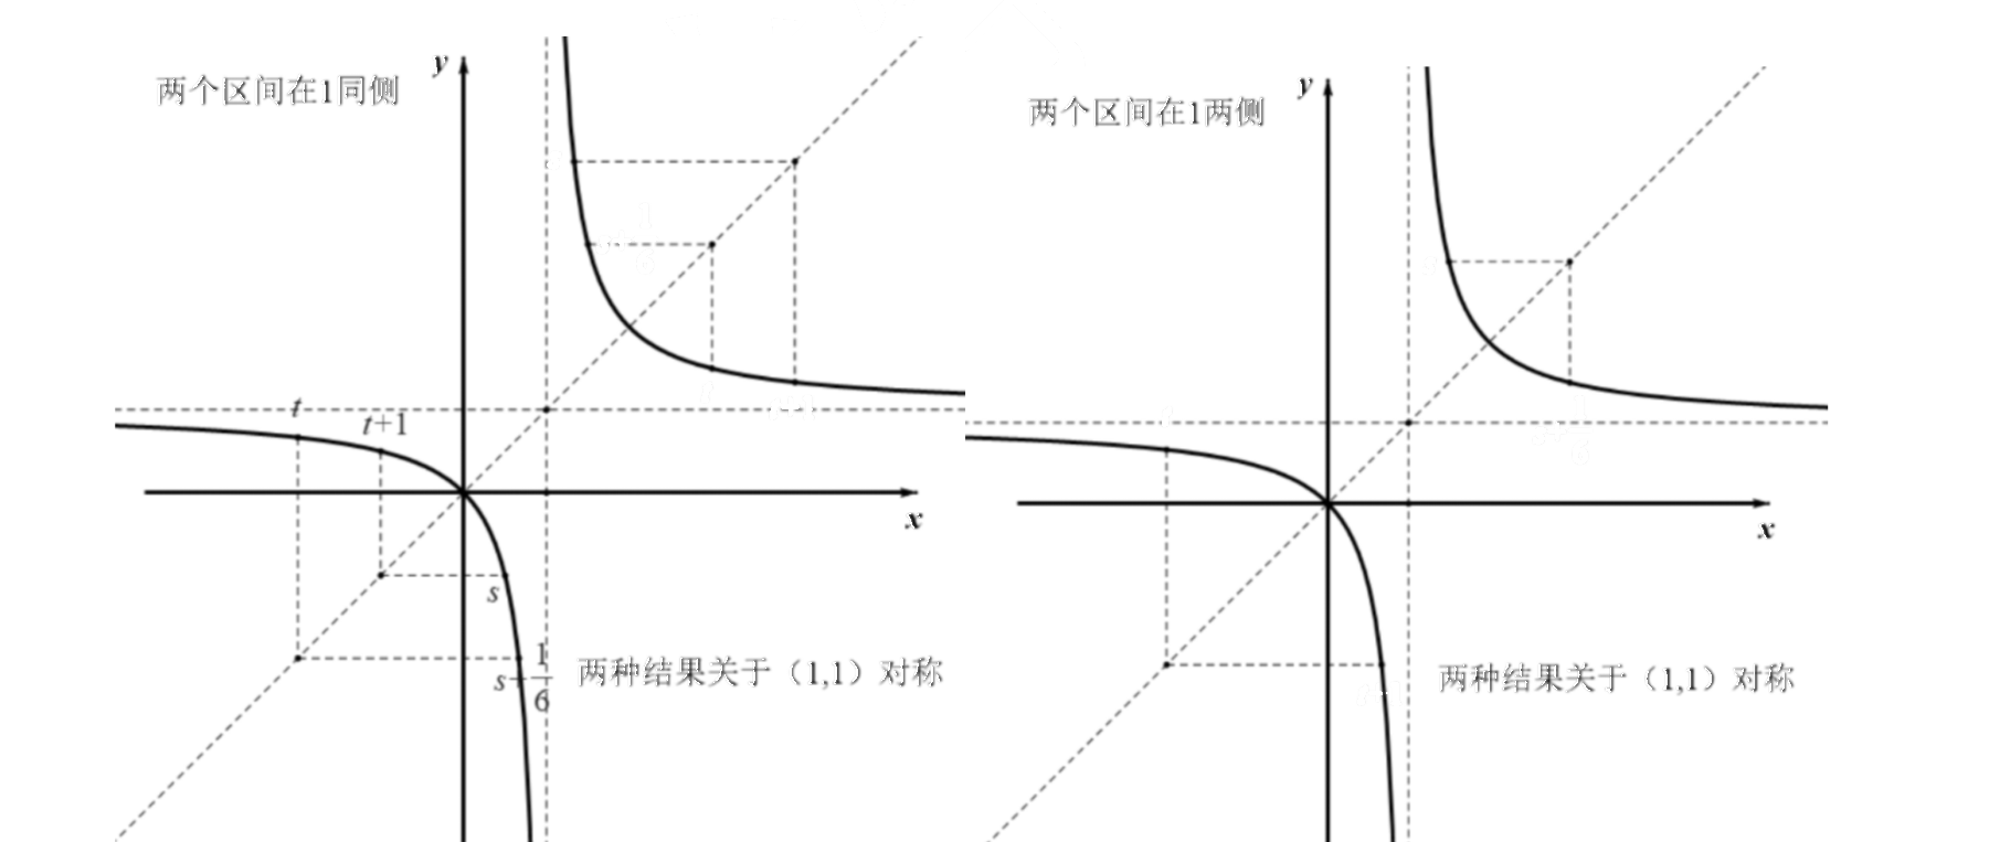
\includegraphics[width=0.92\textwidth]{figures/gao115_q10.png}
\end{center}
\solend
\fi

\end{enumerate}

\bigsec{二、选择题}

\begin{enumerate}
\setcounter{enumi}{10}

\item “对任意有理数 $x$ 都有 $x^2\neq2$”的否定形式是\mbox{（\quad）}% 原卷把答案“$B$”印在题干括号内、无【解析】

\keepwithprev
A. 存在有理数 $x$ 使得 $x^2\neq2$\qquad\qquad B. 存在有理数 $x$ 使得 $x^2=2$

C. 存在无理数 $x$ 使得 $x^2\neq2$\qquad\qquad D. 存在无理数 $x$ 使得 $x^2=2$

\ifanswer
\ans{$B$}
\fi

\item 已知 $a$、$b$ 都是实数，那么“$a^3>b^3$”是“$a^2>b^2$”的\mbox{（\quad）}

\keepwithprev
A. 充分不必要条件\qquad\qquad B. 必要不充分条件

C. 充要条件\qquad\qquad\qquad D. 既不充分也不必要条件

\ifanswer
\solbegin
\step{因为 $a^3>b^3$ 等价于 $a>b$，}
\step{由于 $a$、$b$ 正负不定，所以由 $a>b$ 不能得到 $a^2>b^2$，}
\step{由 $a^2>b^2$ 也不能得到 $a>b$，}
\step{因此“$a^3>b^3$”是“$a^2>b^2$”的既不充分也不必要条件. 故选 $D$.}
\solend
\fi

\item 定义集合运算 $A-B=\{x\mid x\in A$ 且 $x\notin B\}$，将 $A\triangle B=(A-B)\cup(B-A)$ 称为集合 $A$ 与集合 $B$ 的对称差.

命题一：$A\triangle B=B\triangle A$；

命题二：$A\triangle\varnothing=A$；

命题三：$A\cap(B\triangle C)=(A\cap B)\triangle(A\cap C)$；

命题四：$A\cup(B\triangle C)=(A\cup B)\triangle(A\cup C)$；

其中正确命题的个数是\mbox{（\quad）}

\keepwithprev
A. $1$\qquad\qquad B. $2$\qquad\qquad C. $3$\qquad\qquad D. $4$

\ifanswer
\solbegin
\step{对于①，$B\triangle A=(B-A)\cup(A-B)=(A-B)\cup(B-A)=A\triangle B$，①对；}
\step{对于②，$A-B=\{x\mid x\in A$ 且 $x\notin B\}=\{x\mid x\in A$ 且 $x\notin(A\cap B)\}$}
\step{$=A-(A\cap B)$，则 $A\triangle\varnothing=(A-\varnothing)\cup(\varnothing-A)=A\cup\varnothing=A$，②对；}
\step{对于③，$A\cap(B\triangle C)=A\cap(B\cup C-B\cap C)=A\cap(B\cup C)-A\cap(B\cap C)$}
\step{$=(A\cap B)\cup(A\cap C)-(A\cap B)\cap(A\cap C)=(A\cap B)\triangle(A\cap C)$，③对；}
\step{对于④，如图所示：}
\begin{center}
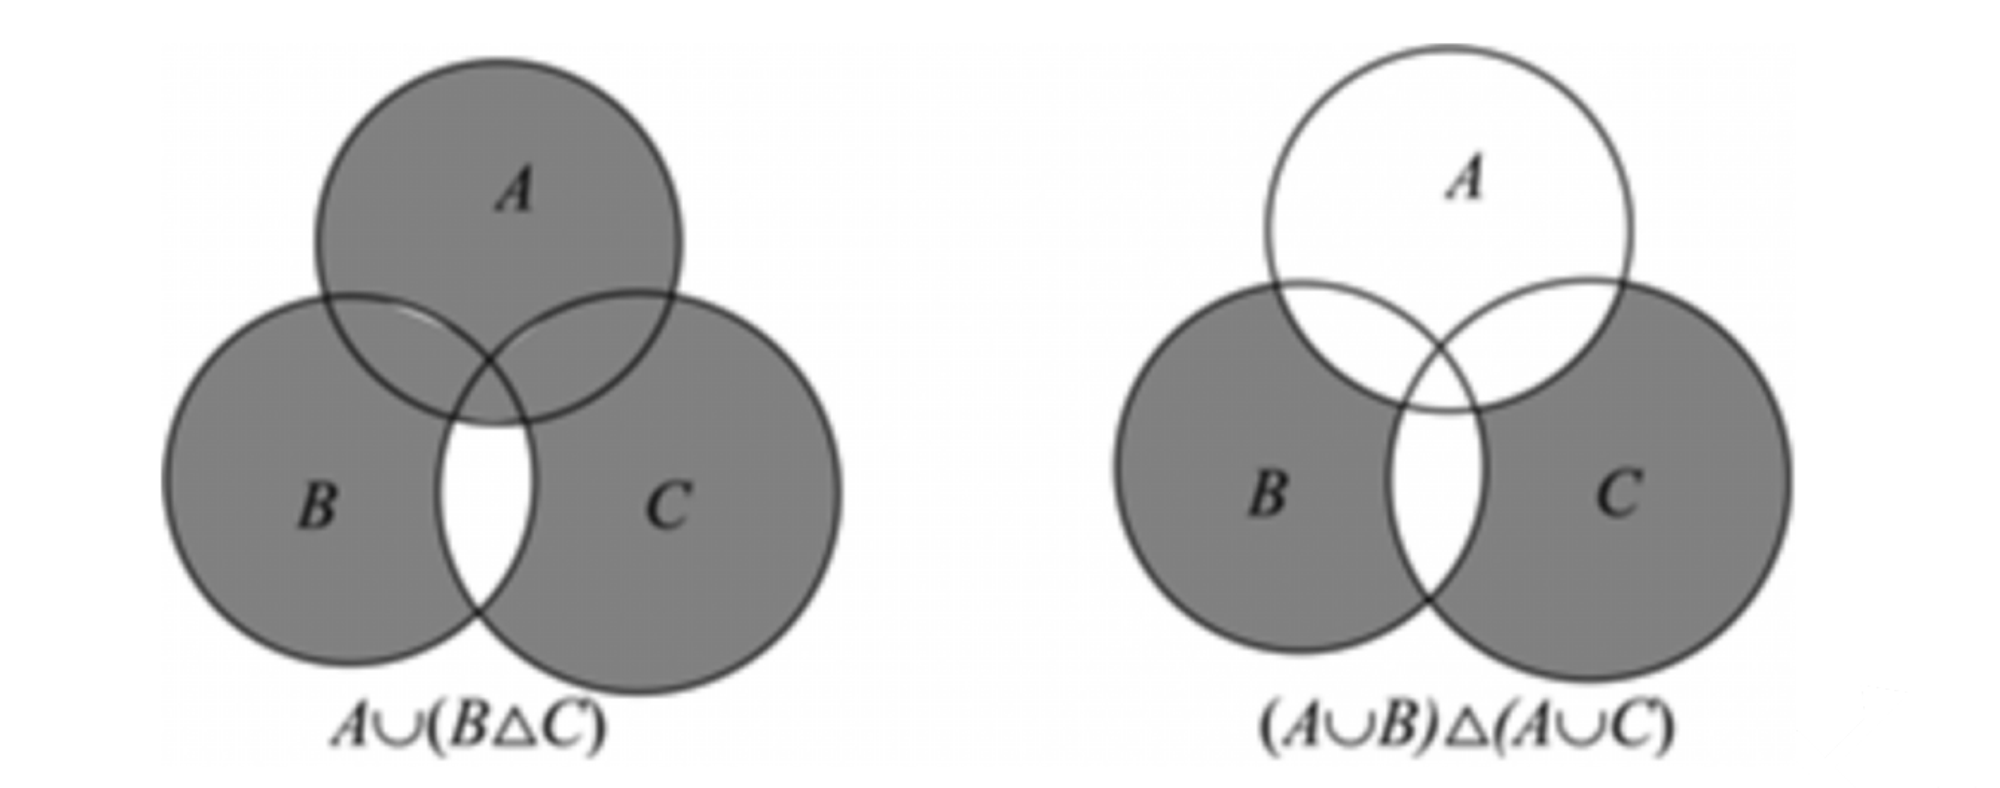
\includegraphics[width=0.85\textwidth]{figures/gao115_q13.png}
\end{center}
\step{所以 $A\cup(B\triangle C)\neq(A\cup B)\triangle(A\cup C)$，④错.}
\step{故选 $C$.}
\solend
\fi

\item 设 $a$、$b$、$c$、$p$ 为实数，若同时满足不等式 $ax^2+bx+c>0$、$bx^2+cx+a>0$ 与 $cx^2+ax+b>0$ 的全体实数 $x$ 所组成的集合等于 $(p,+\infty)$，则关于结论：① $a$、$b$、$c$ 至少有一个为 $0$；② $p=0$. 下列判断中正确的是\mbox{（\quad）}

\keepwithprev
A. ①和②都正确\qquad B. ①和②都错误\qquad C. ①正确，②错误\qquad D. ①错误，②正确

\ifanswer
\solbegin
\step{若同时满足不等式 $ax^2+bx+c>0$、$bx^2+cx+a>0$ 与 $cx^2+ax+b>0$ 的}
\step{全体实数 $x$ 所组成的集合等于 $(p,+\infty)$，必有 $a$,$b$,$c\geqslant0$，}
\step{不妨假设 $a$、$b$、$c$ 没有一个为 $0$，}
\step{则三个不等式均为开口向上的二次函数大于 $0$ 的部分，}
\step{解集的交集应为 $(-\infty,m)\cup(n,+\infty)$ 的形式，矛盾，}
\step{所以 $a$、$b$、$c$ 至少有一个为 $0$，故①正确：}
\step{不妨设 $a=0$，则 $b$,$c\geqslant0$，则不等式组化为 $\begin{cases}bx+c>0\\bx^2+cx>0,\\cx^2+b>0\end{cases}$}
\step{所以 $\begin{cases}x>-\dfrac cb\\x<-\dfrac cb\text{或}x>0\\x\in\R\end{cases}$，取交集得 $(0,+\infty)$，故 $p=0$，故②正确：}
\step{故选 $A$.}
\solend
\fi

\end{enumerate}

\bigsec{三、解答题}

\begin{enumerate}
\setcounter{enumi}{14}

\item 已知 $a>0$，$b>0$，

（1）试比较 $\dfrac{a^2-b^2}{a^2+b^2}$ 与 $\dfrac{a-b}{a+b}$ 的大小；

（2）若 $a+b>4$，求证：$\dfrac a{b+2}$ 和 $\dfrac b{a+2}$ 中至少有一个大于 $\dfrac12$.

\ifanswer
\solbegin
\step{（1）已知 $a>0$，$b>0$，$\dfrac{a^2-b^2}{a^2+b^2}-\dfrac{a-b}{a+b}=\dfrac{2ab(a-b)}{(a^2+b^2)(a+b)}$，}
\step{当 $a>b$ 时，$a-b>0$，所以 $\dfrac{a^2-b^2}{a^2+b^2}-\dfrac{a-b}{a+b}>0$，所以 $\dfrac{a^2-b^2}{a^2+b^2}>\dfrac{a-b}{a+b}$；}
\step{当 $a=b$ 时，$a-b=0$，所以 $\dfrac{a^2-b^2}{a^2+b^2}-\dfrac{a-b}{a+b}=0$，所以 $\dfrac{a^2-b^2}{a^2+b^2}=\dfrac{a-b}{a+b}$；}
\step{当 $a<b$ 时，$a-b<0$，所以 $\dfrac{a^2-b^2}{a^2+b^2}-\dfrac{a-b}{a+b}<0$，所以 $\dfrac{a^2-b^2}{a^2+b^2}<\dfrac{a-b}{a+b}$；}
\step{（2）假设 $\dfrac a{b+2}$ 和 $\dfrac b{a+2}$ 中都不大于 $\dfrac12$，即 $\dfrac b{a+2}\leqslant\dfrac12$，$\dfrac a{b+2}\leqslant\dfrac12$，}
\step{因为 $a>0$，$b>0$，所以 $a+2>0$，$b+2>0$，}
\step{所以 $2b\leqslant a+2$，$2a\leqslant b+2$，}
\step{两式相加得 $2a+2b\leqslant a+2+b+2=a+b+4$，即 $a+b\leqslant4$，}
\step{与已知 $a+b>4$ 矛盾，所以假设错误，}
\step{故 $\dfrac a{b+2}$ 和 $\dfrac b{a+2}$ 中至少有一个大于 $\dfrac12$.}
\solend
\fi

\item 某企业原有 $200$ 名科技人员，年人均工资 $a$ 万元($a>0$). 现加大对某芯片研发力度，该企业把原有 $200$ 名科技人员调整成技术人员和研发人员，其中技术人员 $x$ 名($x\in\N$ 且 $40\leqslant x\leqslant80$). 调整后，研发人员的年人均工资比调整前增加了 $(2x)\%$，技术人员的年人均工资为 $a\left(m-\dfrac x{10}\right)$万元.

（1）若要使调整后研发人员的年总工资不低于调整前 $200$ 名科技人员年总工资的 $1.5$ 倍，求调整后的技术人员最少有多少人？

（2）为了激励研发人员的工作热情和保持技术人员的工作积极性，企业决定在工资方面要同时满足以下两个条件：

①研发人员的年总工资始终不低于技术人员的年总工资；

②技术人员的年人均工资始终不低于调整前 $200$ 名科技人员的年人均工资.

请问是否存在这样的实数 $m$？若存在，求出 $m$ 的范围；若不存在，说明理由.

\ifanswer
\solbegin
\step{（1）由题意得调整后研发人员的年人均工资为 $[1+(2x)\%]a$ 万元，}
\step{那么 $(200-x)[1+(2x)\%]a\geqslant1.5\times200a$ ($a>0$)，}
\step{化简得 $x^2-150x+5000\leqslant0$，解得 $50\leqslant x\leqslant100$，}
\step{由于 $x\in\N$ 且 $40\leqslant x\leqslant80$，因此 $50\leqslant x\leqslant80$，}
\step{因此调整后的技术人员的人数最少为 $50$ 人；}
\step{（2）假设存在实数 $m$，使得技术人员在已知范围内调整后，满足以上两个条件，}
\step{由条件①得 $(200-x)[1+(2x)\%]a\geqslant x\left(m-\dfrac x{10}\right)a$，}
\step{整理得 $m\leqslant\dfrac{200}{x}+\dfrac{2x}{25}+3$；}
\step{因为 $\dfrac{200}{x}+\dfrac{2x}{25}+3\geqslant2\sqrt{\dfrac{200}{x}\cdot\dfrac{2x}{25}}+3=11$，}
\step{当且仅当 $\dfrac{200}{x}=\dfrac{2x}{25}$，即 $x=50$ 时取等号，因此 $m\leqslant11$，}
\step{由条件②得 $a\left(m-\dfrac x{10}\right)\geqslant a$，所以 $m\geqslant\dfrac x{10}+1$；}
\step{又由于 $40\leqslant x\leqslant80$，因此 $m\geqslant9$.}
\step{因此 $m\in[9,11]$.}
\solend
\fi

\item 已知 $a\in\R$，记 $f(x)=ax^2-(a+2)x+2$.

（1）若 $f(x)<3-2x$ 对于一切 $x\in\R$ 恒成立，求实数 $a$ 的取值范围；

（2）求关于 $x$ 不等式 $f(x)\geqslant0$ 的解集；

（3）若存在 $m\in\R$ 使关于 $x$ 的方程 $ax^2-(a+2)\lvert x\rvert+2=\lvert m+2\rvert+\lvert m-1\rvert$ 有四个不同的实根，求实数 $a$ 的取值范围.

\ifanswer
\solbegin
\step{（1）由 $f(x)<3-2x$ 对于一切 $x\in\R$ 恒成立，}
\step{得 $ax^2-ax-1<0$ 对于一切 $x\in\R$ 恒成立，}
\step{当 $a=0$ 时，原式可化为 $-1<0$，恒成立，符合条件；}
\step{当 $a\neq0$ 时，需满足 $\begin{cases}a<0\\\Delta=a^2+4a<0\end{cases}$，解得 $-4<a<0$；}
\step{综上，实数 $a$ 的取值范围是 $(-4,0]$；}
\step{（2）$f(x)\geqslant0$，即 $(ax-2)(x-1)\geqslant0$，}
\step{当 $a=0$ 时，原式化为 $-2x+2\geqslant0$，解集为 $\{x\mid x\leqslant1\}$；}
\step{当 $a>0$ 时，若 $a=2$，原式化为 $2(x-1)^2\geqslant0$，解集为 $\R$；}
\step{若 $0<a<2$，$\dfrac2a>1$，解集为 $\{x\mid x\leqslant1$ 或 $x\geqslant\dfrac2a\}$；}
\step{若 $a>2$，$\dfrac2a<1$，解集为 $\{x\mid x\leqslant\dfrac2a$ 或 $x\geqslant1\}$；}
\step{当 $a<0$ 时，$\dfrac2a<1$，解集为 $\left\{x\,\middle\vert\,\dfrac2a\leqslant x\leqslant1\right\}$；}
\step{综上，当 $a<0$ 时，不等式解集为 $\left\{x\,\middle\vert\,\dfrac2a\leqslant x\leqslant1\right\}$；}
\step{当 $a=0$ 时，不等式解集为 $\{x\mid x\leqslant1\}$；}
\step{当 $0<a<2$ 时，不等式解集为 $\{x\mid x\leqslant1$ 或 $x\geqslant\dfrac2a\}$；}
\step{当 $a=2$ 时，不等式解集为 $\R$；}
\step{当 $a>2$ 时，不等式解集为 $\{x\mid x\leqslant\dfrac2a$ 或 $x\geqslant1\}$；}
\step{（3）由绝对值三角不等式得 $\lvert m+2\rvert+\lvert m-1\rvert\geqslant\lvert(m+2)-(m-1)\rvert=3$，}
\step{即右侧取值范围为 $[3,+\infty)$，}
\step{令 $t=\lvert x\rvert\geqslant0$，原方程转化为 $at^2-(a+2)t+2=k$，$k\in[3,+\infty)$，}
\step{若原方程有四个不同实根，}
\step{需存在 $k\geqslant3$，使得方程 $at^2-(a+2)t+2-k=0$ 有两个不同正实根，}
\step{当 $a\geqslant0$ 时，方程的两根之积为 $\dfrac{2-k}{a}$，}
\step{因为 $k\geqslant3$，所以 $2-k\leqslant-1<0$，两根一正一负，}
\step{最多只有一个正根，对应最多两个 $x$ 根，不符合要求；}
\step{当 $a<0$ 时，两根之积为正，}
\step{要两个根都为正，需要两根之和 $\dfrac{a+2}{a}>0$，解得 $a<-2$，}
\step{再要求存在 $k\geqslant3$ 使得判别式大于 $0$，}
\step{即 $\triangle=(a+2)^2-4a(2-k)>0$ 在 $k\in[3,+\infty)$ 上有解，}
\step{即 $(a-2)^2+4ak>0$ 在 $k\in[3,+\infty)$ 上有解，}
\step{由 $a<0$，得 $(a-2)^2+12a>0$，}
\step{即 $a^2+8a+4>0$，结合 $a<-2$ 解得 $a<-4-2\sqrt3$，}
\step{故实数 $a$ 的取值范围是 $(-\infty,-4-2\sqrt3)$.}
\solend
\fi

\item 设 $A=\{x_1,x_2,\cdots,x_n\}(n\geqslant2,n\in\N)$，且 $x_1,x_2,\cdots,x_n$ 均为正整数，若对于 $A$ 中任意两个元素 $a,b$，当 $a>b$ 时，都有 $\dfrac{b^2}{a-b}\in A$，则称 $A$ 为“$n$ 元好集”.

（1）判断 $\{2,4,6\}$ 是否为“三元好集”，并说明理由；

（2）若集合 $M$ 为“二元好集”，且 $M$ 中所有元素之积小于 $2026$，求所有满足条件的集合 $M$ 的个数；

（3）设 $k\geqslant3,k\in\N$，是否存在“$k$ 元好集”，若存在，求出所有满足条件的“$k$ 元好集”，若不存在，请说明理由.

\ifanswer
\solbegin
\step{（1）取 $a=6,b=2$，则 $\dfrac{b^2}{a-b}=\dfrac44=1\notin\{2,4,6\}$，所以该集合不是三元好集.}
\step{（2）设 $M=\{b,a\}$，其中 $a>b$ 且均为正整数，则 $\dfrac{b^2}{a-b}$ 等于 $a$ 或 $b$.}
\step{若 $\dfrac{b^2}{a-b}=a$，则 $a^2-ab-b^2=0$，从而 $\dfrac ab=\dfrac{1+\sqrt5}{2}$，与 $\dfrac ab$ 为有理数矛盾.}
\step{若 $\dfrac{b^2}{a-b}=b$，则 $a=2b$；}
\step{反之，任意正整数 $b$ 对应的 $\{b,2b\}$ 均为二元好集.}
\step{由元素之积小于 $2026$，得 $2b^2<2026\Leftrightarrow b^2<1013$.}
\step{因为 $31^2=961<1013<1024=32^2$，所以 $b=1,2,\cdots,31$，}
\step{对应 $31$ 个不同的集合.}
\step{（3）假设存在 $k\geqslant3$ 的 $k$ 元好集 $A$，将其元素从小到大排列，}
\step{记最小元素为 $u$，次小元素为 $v$，最大元素为 $w$，则 $0<u<v<w$.}
\step{由 $\dfrac{u^2}{w-u}\in A$，该数不小于 $u$，得 $\dfrac{u^2}{w-u}\geqslant u\Rightarrow w\leqslant2u$.}
\step{又由 $\dfrac{u^2}{v-u}$,$\dfrac{v^2}{w-v}\in A$，这两个数均不超过 $w$，}
\step{得 $\dfrac{u^2}{v-u}\leqslant w$,$\dfrac{v^2}{w-v}\leqslant w$，}
\step{分母均为正，分别去分母后相加，}
\step{得 $u^2+v^2\leqslant w(v-u)+w(w-v)=w(w-u)\leqslant2u^2$，}
\step{于是 $v^2\leqslant u^2$，与 $v>u>0$ 矛盾，所以不存在 $k\geqslant3$ 的 $k$ 元好集.}
\solend
\fi

\end{enumerate}

\end{document}
"
% 紧凑版：xelatex "\def\iscompact{1}% 高一115_复旦附中_10月阶段练习.tex
%   —— 高一上数学“2026-2027 年复旦附中高一上 10 月阶段练习”（试卷版/答案版）
% 试卷版：xelatex 高一115_复旦附中_10月阶段练习.tex
% 答案版：xelatex "\def\isanswer{1}% 高一115_复旦附中_10月阶段练习.tex
%   —— 高一上数学“2026-2027 年复旦附中高一上 10 月阶段练习”（试卷版/答案版）
% 试卷版：xelatex 高一115_复旦附中_10月阶段练习.tex
% 答案版：xelatex "\def\isanswer{1}\input{高一115_复旦附中_10月阶段练习.tex}"
% 紧凑版：xelatex "\def\iscompact{1}\input{高一115_复旦附中_10月阶段练习.tex}"
%
% 原始材料：微信公众号“魔都数学加油站”文章，作者破晓，2026-11-06 17:58 发布；
% 连载“27学年高一115”，原文标题“27学年高一115——2026-2027年上海市复旦附中高一上10月阶段练习”；
% 原文链接：https://mp.weixin.qq.com/s/krocP0fMQQ4VM1SQEcLI2Q。
% 正文为 12 张 PNG 页（第 4、6、12 页 2560×3620，其余 4762×6735），
% 题目下印有【解析】或【答案】，为讲评版。
% 题目、解析均据原图转录；卷面红色水印及公众号页脚未录入。
%
% 卷首标题：原卷印作“2026-2027 年复旦附中高一上 10 月阶段练习”（公众号标题中的“上海市”
% 卷面标题行没有，本稿照卷面），年份区间按全稿惯例排 en dash；原卷未印副标题，本稿按题目内容
% 标为“集合与常用逻辑用语、不等式”。
%
% 与原卷的排版差异：
%   ① 原文从第 3 题起，填空题编号为 3—10、选择题为 11—14、解答题为 15—18，共 16 题，
%      本稿保留原题号（与多数卷的 3—21 不同）；
%   ② 原卷每题下直接印【解析】／【答案】，本稿按全稿惯例置于答案版；第 11 题把答案“$B$”
%      印在题干括号内且无【解析】，另提 \ans{}；其余选择题答案在解析末句“故选 …”，括号内留空；
%   ③ 原卷未印副标题，本稿按“知识模块”口径补出；
%   ④ 原卷填空横线按全稿惯例排为 \blankline[4.4em]；选择题括号排 \mbox{（\quad）}、
%      选项段前按惯例加 \keepwithprev；解答题不留作答区（原卷为讲评版，与 109—114 同）；
%   ⑤ 原卷数集排斜体 $R$／$Q$／$N$，按全稿惯例改 \R、\Q、\N。
%
% 判别式与对称差字形：原卷 $\triangle$（等边、扁）与 $\Delta$（等腰、高）两种混用，逐处照录——
%   第 7 题与第 17 题 (3) 的判别式、第 13 题的对称差 $A\triangle B$ 用 \triangle，
%   第 17 题 (1) cases 的判别式用 \Delta。
%
% 子集符号：第 4 题解析的 $(-1,3)\subset(-m,m)$ 印单线（真子集、无下划线），按 18／96
%   成例照录 \subset；第 5 题解析的 $B\subseteq A$ 印有下划线，照录 \subseteq。
%   第 3 题的补集照原卷上划线排 \overline{N}。
%
% 原卷存疑照录：第 9 题解析末行“故可能成立的是①②③”与四种情形的编号一致，照录；
%   第 10 题解析两幅函数图上另有蓝色／红色手写标注（$t$、$t+1$、$s$、$\frac16$ 等），
%   系批改笔迹，随裁图保留、不另作正文录入；第 14 题解析的 cases 三行照原卷排；
%   第 18 题 (2) 解析“所以该集合不是三元好集”前的取例 $a=6,b=2$ 照录。
%
% 行数核对：逐题数 \step/\stepm 条数，合计 133 条（Q3：3；Q4：3；Q5：4；Q6：5；Q7：4；
% Q8：4；Q9：11；Q10：7；Q11：0；Q12：4；Q13：8；Q14：9；Q15：10；Q16：13；
% Q17：32；Q18：16），与原卷印刷行逐题相等（cases 块作一个印刷行计）。第 11 题括号内印
% 答案且无解析，提 \ans{}，不计入 \step 账；第 10、13 题解析内的插图不计入 \step 账。
%
\documentclass[a4paper,11pt]{article}
\usepackage{common}

\begin{document}

\examtitlest[3]{2026--2027 年复旦附中高一上 10 月阶段练习}{集合与常用逻辑用语、不等式}

\bigsec{一、填空题}

\begin{enumerate}
\setcounter{enumi}{2}

\item 已知集合 $M=\{x\mid 4x^2-4x-15>0\}$，$N=\left\{x\,\middle\vert\,\dfrac{x+1}{x-6}>0\right\}$，则 $M\cap\overline{N}=$\blankline[4.4em].

\ifanswer
\solbegin
\step{集合 $M=\{x\mid 4x^2-4x-15>0\}=\{x\mid x>\dfrac52$ 或 $x<-\dfrac32\}$，}
\step{$N=\left\{x\,\middle\vert\,\dfrac{x+1}{x-6}>0\right\}=\{x\mid x>6$ 或 $x<-1\}$，得 $\overline{N}=\{x\mid-1\leqslant x\leqslant6\}$，}
\step{故 $M\cap\overline{N}=\left\{x\,\middle\vert\,\dfrac52<x\leqslant6\right\}$.}
\solend
\fi

\item 已知 $m>0$，不等式 $\lvert x\rvert<m$ 成立的一个充分不必要条件是 $-1<x<3$，则 $m$ 的取值范围是\blankline[4.4em].

\ifanswer
\solbegin
\step{不等式 $-m<x<m$ 成立的一个充分不必要条件是 $-1<x<3$，}
\step{由题意得 $(-1,3)\subset(-m,m)$，则 $m\geqslant3$，此时 $-m\leqslant-3<-1$，}% 原卷印单线 \subset，照录
\step{所以 $m$ 的取值范围是 $\{m\mid m\geqslant3\}$.}
\solend
\fi

\item 已知集合 $A=\{1,2\}$，集合 $B=\{x\mid ax=6\}$，若 $A\cup B=A$，则 $a$ 的所有取值构成的集合为\blankline[4.4em].

\ifanswer
\solbegin
\step{因为 $A\cup B=A$，所以 $B\subseteq A$，}
\step{当 $a=0$ 时，$B=\varnothing$，满足 $B\subseteq A$；}
\step{当 $a\neq0$ 时，$B=\left\{\dfrac6a\right\}$，则 $\dfrac6a=1$ 或 $\dfrac6a=2$，解得 $a=6$ 或 $a=3$，}
\step{综上所述，$a$ 的所有取值构成的集合为 $\{0,3,6\}$.}
\solend
\fi

\item 若关于 $x$ 的不等式 $ax^2+bx+c>0$ 的解集为 $(-3,2)$，则不等式 $ax^2+(a+b)x+c-2a>0$ 的解集为\blankline[4.4em].

\ifanswer
\solbegin
\step{由 $ax^2+bx+c>0$ 的解集为 $(-3,2)$ 得 $a<0$，}
\step{且 $ax^2+bx+c=0$ 时 $x_1=-3$，$x_2=2$，}
\step{得 $-3+2=-\dfrac ba$，即 $b=a$，$-3\times2=\dfrac ca$，即 $c=-6a$，}
\step{代入 $ax^2+(a+b)x+c-2a>0$ 得 $ax^2+2ax-8a>0$ 化简得 $x^2+2x-8<0$，}
\step{解得 $-4<x<2$，故解集为 $(-4,2)$.}
\solend
\fi

\item 已知关于 $x$ 的方程 $x^2-2x+m=0$ 的两个实数根分别为 $x_1$，$x_2$. 若 $x_1^2x_2^2+x_1^2+x_2^2=7$，则实数 $m$ 的值为\blankline[4.4em].

\ifanswer
\solbegin
\step{由韦达定理得 $x_1+x_2=2$，$x_1x_2=m$，}
\step{$x_1^2x_2^2+x_1^2+x_2^2=(x_1x_2)^2+(x_1+x_2)^2-2x_1x_2=m^2+4-2m$，}
\step{由 $m^2+4-2m=7$，得 $m^2-2m-3=0$，解得 $m=3$ 或 $m=-1$，}
\step{方程有两个实数根，故 $\triangle=4-4m\geqslant0$，即 $m\leqslant1$，所以 $m=-1$.}
\solend
\fi

\item 已知 $x>1$，若 $x^2-xy+y=0$，则 $x+y$ 的最小值是\blankline[4.4em].

\ifanswer
\solbegin
\step{由于 $x^2-xy+y=0$，则 $y=\dfrac{x^2}{x-1}>0$，}
\step{则 $x+y=x+\dfrac{x^2}{x-1}=\dfrac{2x^2-x}{x-1}=\dfrac{2(x-1)^2+3(x-1)+1}{x-1}$}
\step{$=2(x-1)+\dfrac1{x-1}+3\geqslant2\sqrt{2(x-1)\cdot\dfrac1{x-1}}+3=2\sqrt2+3$，}
\step{当且仅当 $x=1+\dfrac{\sqrt2}{2}$ 时取等号，故最小值是 $2\sqrt2+3$.}
\solend
\fi

\item 若集合 $A=B_1\cup B_2\cup\cdots\cup B_n$，其中 $B_1$、$B_2$、$\cdots$、$B_n$ 为非空集合，$B_i\cap B_j=\varnothing$，$1\leqslant i<j\leqslant n$，则称集合 $\{B_1,B_2,\cdots,B_n\}$ 为集合 $A$ 的一个 $n$ 划分. 例如：集合 $\{\{1,2\},\{3\}\}$，$\{\{1,3\},\{2\}\}$，$\{\{2,3\},\{1\}\}$ 均为集合 $\{1,2,3\}$ 的一个 $2$ 划分. 设 $\{B_1,B_2\}$ 为有理数集 $\Q$ 的一个 $2$ 划分，且满足对任意 $x\in B_1$，任意 $y\in B_2$，都有 $x<y$. 则对于 $B_1$、$B_2$ 有：

① $B_1$ 中的元素存在最大值，$B_2$ 中的元素不存在最小值；

② $B_1$ 中的元素不存在最大值，$B_2$ 中的元素存在最小值；

③ $B_1$ 中的元素不存在最大值，$B_2$ 中的元素不存在最小值；

④ $B_1$ 中的元素存在最大值，$B_2$ 中的元素存在最小值；

对于以上四种情况，可能成立的序号有\blankline[4.4em].

\ifanswer
\solbegin
\step{对于①，$B_1=\{x\in\Q\mid x\leqslant2\}$，$B_2=\{x\in\Q\mid x>2\}$，①可能成立；}
\step{对于②，$B_1=\{x\in\Q\mid x<2\}$，$B_2=\{x\in\Q\mid x\geqslant2\}$，②可能成立；}
\step{对于③，$B_1=\{x\in\Q\mid x<\pi\}$，$B_2=\{x\in\Q\mid x>\pi\}$，③可能成立；}
\step{对于④，假设④成立，}
\step{不妨设 $B_1$ 中的元素的最大值为 $s$，$B_2$ 中的元素的最小值为 $t$，}
\step{由题意得 $s<t$，所以 $s<\dfrac{s+t}{2}<t$，}
\step{因为 $s$ 为 $B_1$ 中的元素的最大值，所以 $\dfrac{s+t}{2}\notin B_1$，}
\step{因为 $t$ 为 $B_2$ 中的元素的最小值，所以 $\dfrac{s+t}{2}\notin B_2$，}
\step{又 $B_1\cup B_2=\Q$，所以 $\dfrac{s+t}{2}\notin\Q$，与 $\dfrac{s+t}{2}\in\Q$ 矛盾，}
\step{所以假设不成立，即④不可能成立.}
\step{故可能成立的是①②③.}
\solend
\fi

\item 已知集合 $A=\left[s,s+\dfrac16\right]\cup[t,t+1]$，其中 $1\notin A$ 且 $s+\dfrac16<t$，函数 $f(x)=\dfrac x{x-1}$，且对任意 $a\in A$，都有 $f(a)\in A$，则 $t$ 的值是\blankline[4.4em].

\ifanswer
\solbegin
\step{若 $\left[s,s+\dfrac16\right]$,$[t,t+1]$ 在 $f(x)=\dfrac x{x-1}$ 图像的同侧，}
\step{则点 $\left(t,s+\dfrac16\right)$,$(t+1,s)$ 在 $f(x)=\dfrac x{x-1}$ 的图像上，}
\step{所以 $\dfrac t{t-1}=\dfrac{t+1}{t}+\dfrac16$，解得 $t=-2$ 或 $t=3$，检验得 $t=3$；}
\step{若 $\left[s,s+\dfrac16\right]$,$[t,t+1]$ 在 $f(x)=\dfrac x{x-1}$ 图像的两侧，}
\step{则点 $(t,t+1)$ 在 $f(x)=\dfrac x{x-1}$ 的图像上，}
\step{所以 $t+1=\dfrac t{t-1}$，解得 $t=\dfrac{1\pm\sqrt5}{2}$，检验得 $t=\dfrac{1+\sqrt5}{2}$，}
\step{综上，$t=\dfrac{1+\sqrt5}{2}$ 或 $t=3$.}
\begin{center}
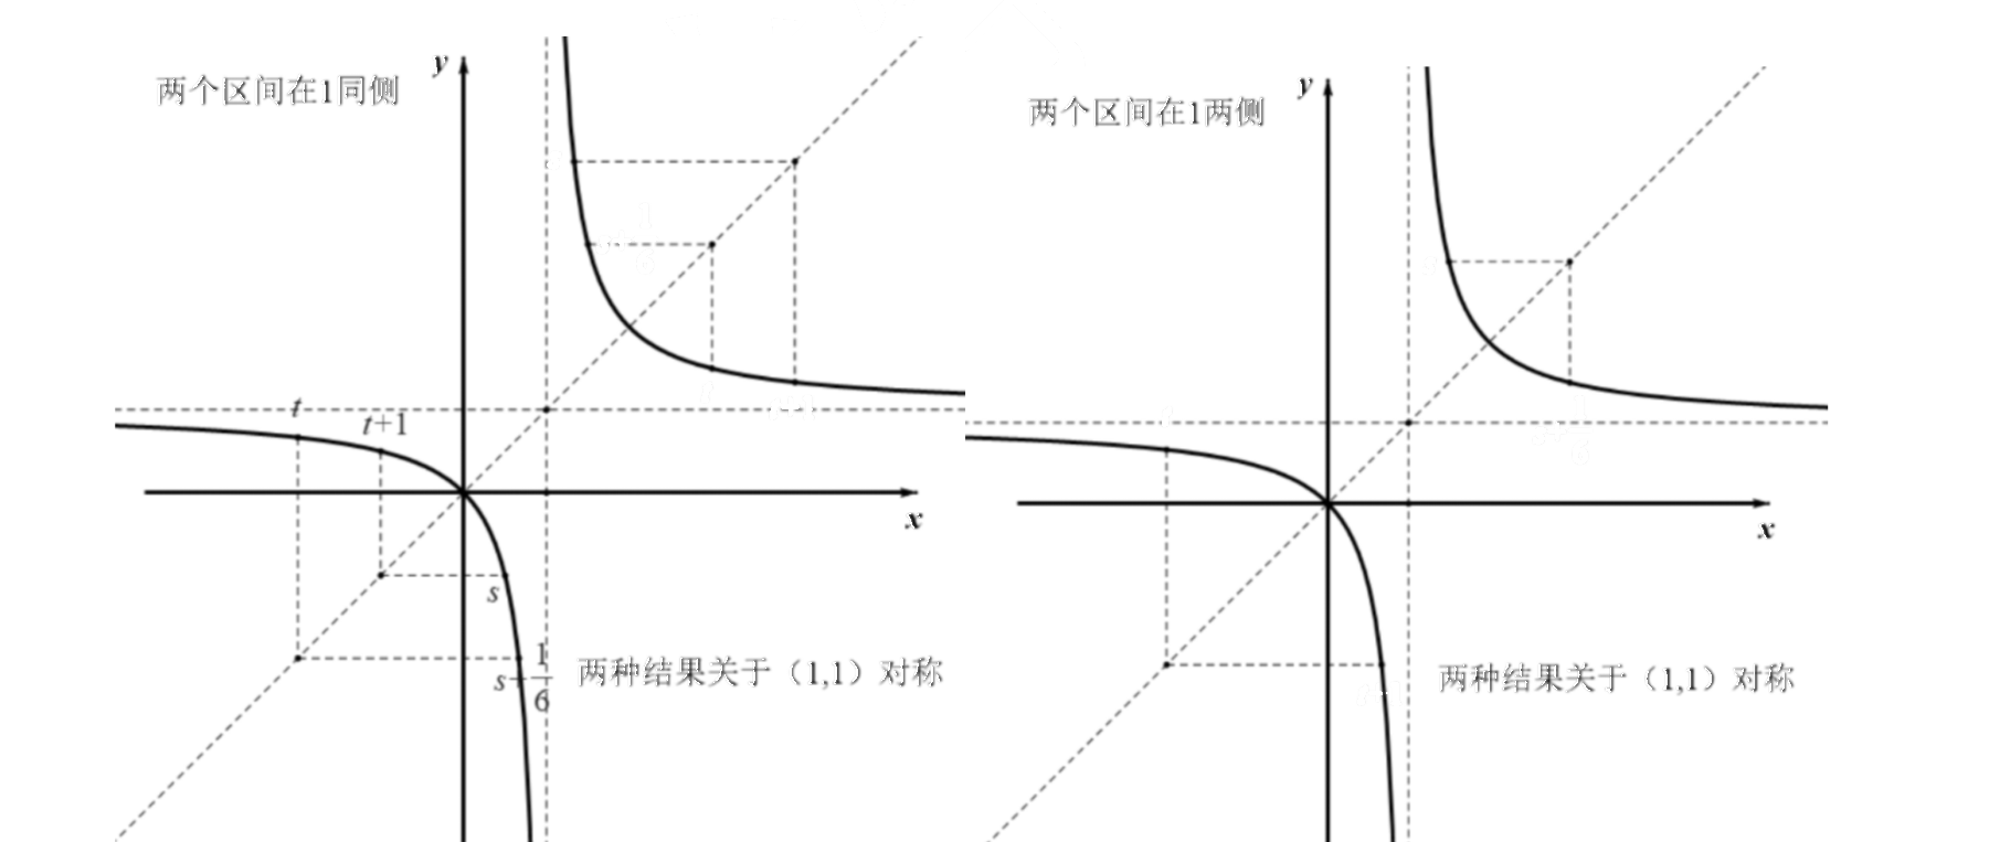
\includegraphics[width=0.92\textwidth]{figures/gao115_q10.png}
\end{center}
\solend
\fi

\end{enumerate}

\bigsec{二、选择题}

\begin{enumerate}
\setcounter{enumi}{10}

\item “对任意有理数 $x$ 都有 $x^2\neq2$”的否定形式是\mbox{（\quad）}% 原卷把答案“$B$”印在题干括号内、无【解析】

\keepwithprev
A. 存在有理数 $x$ 使得 $x^2\neq2$\qquad\qquad B. 存在有理数 $x$ 使得 $x^2=2$

C. 存在无理数 $x$ 使得 $x^2\neq2$\qquad\qquad D. 存在无理数 $x$ 使得 $x^2=2$

\ifanswer
\ans{$B$}
\fi

\item 已知 $a$、$b$ 都是实数，那么“$a^3>b^3$”是“$a^2>b^2$”的\mbox{（\quad）}

\keepwithprev
A. 充分不必要条件\qquad\qquad B. 必要不充分条件

C. 充要条件\qquad\qquad\qquad D. 既不充分也不必要条件

\ifanswer
\solbegin
\step{因为 $a^3>b^3$ 等价于 $a>b$，}
\step{由于 $a$、$b$ 正负不定，所以由 $a>b$ 不能得到 $a^2>b^2$，}
\step{由 $a^2>b^2$ 也不能得到 $a>b$，}
\step{因此“$a^3>b^3$”是“$a^2>b^2$”的既不充分也不必要条件. 故选 $D$.}
\solend
\fi

\item 定义集合运算 $A-B=\{x\mid x\in A$ 且 $x\notin B\}$，将 $A\triangle B=(A-B)\cup(B-A)$ 称为集合 $A$ 与集合 $B$ 的对称差.

命题一：$A\triangle B=B\triangle A$；

命题二：$A\triangle\varnothing=A$；

命题三：$A\cap(B\triangle C)=(A\cap B)\triangle(A\cap C)$；

命题四：$A\cup(B\triangle C)=(A\cup B)\triangle(A\cup C)$；

其中正确命题的个数是\mbox{（\quad）}

\keepwithprev
A. $1$\qquad\qquad B. $2$\qquad\qquad C. $3$\qquad\qquad D. $4$

\ifanswer
\solbegin
\step{对于①，$B\triangle A=(B-A)\cup(A-B)=(A-B)\cup(B-A)=A\triangle B$，①对；}
\step{对于②，$A-B=\{x\mid x\in A$ 且 $x\notin B\}=\{x\mid x\in A$ 且 $x\notin(A\cap B)\}$}
\step{$=A-(A\cap B)$，则 $A\triangle\varnothing=(A-\varnothing)\cup(\varnothing-A)=A\cup\varnothing=A$，②对；}
\step{对于③，$A\cap(B\triangle C)=A\cap(B\cup C-B\cap C)=A\cap(B\cup C)-A\cap(B\cap C)$}
\step{$=(A\cap B)\cup(A\cap C)-(A\cap B)\cap(A\cap C)=(A\cap B)\triangle(A\cap C)$，③对；}
\step{对于④，如图所示：}
\begin{center}
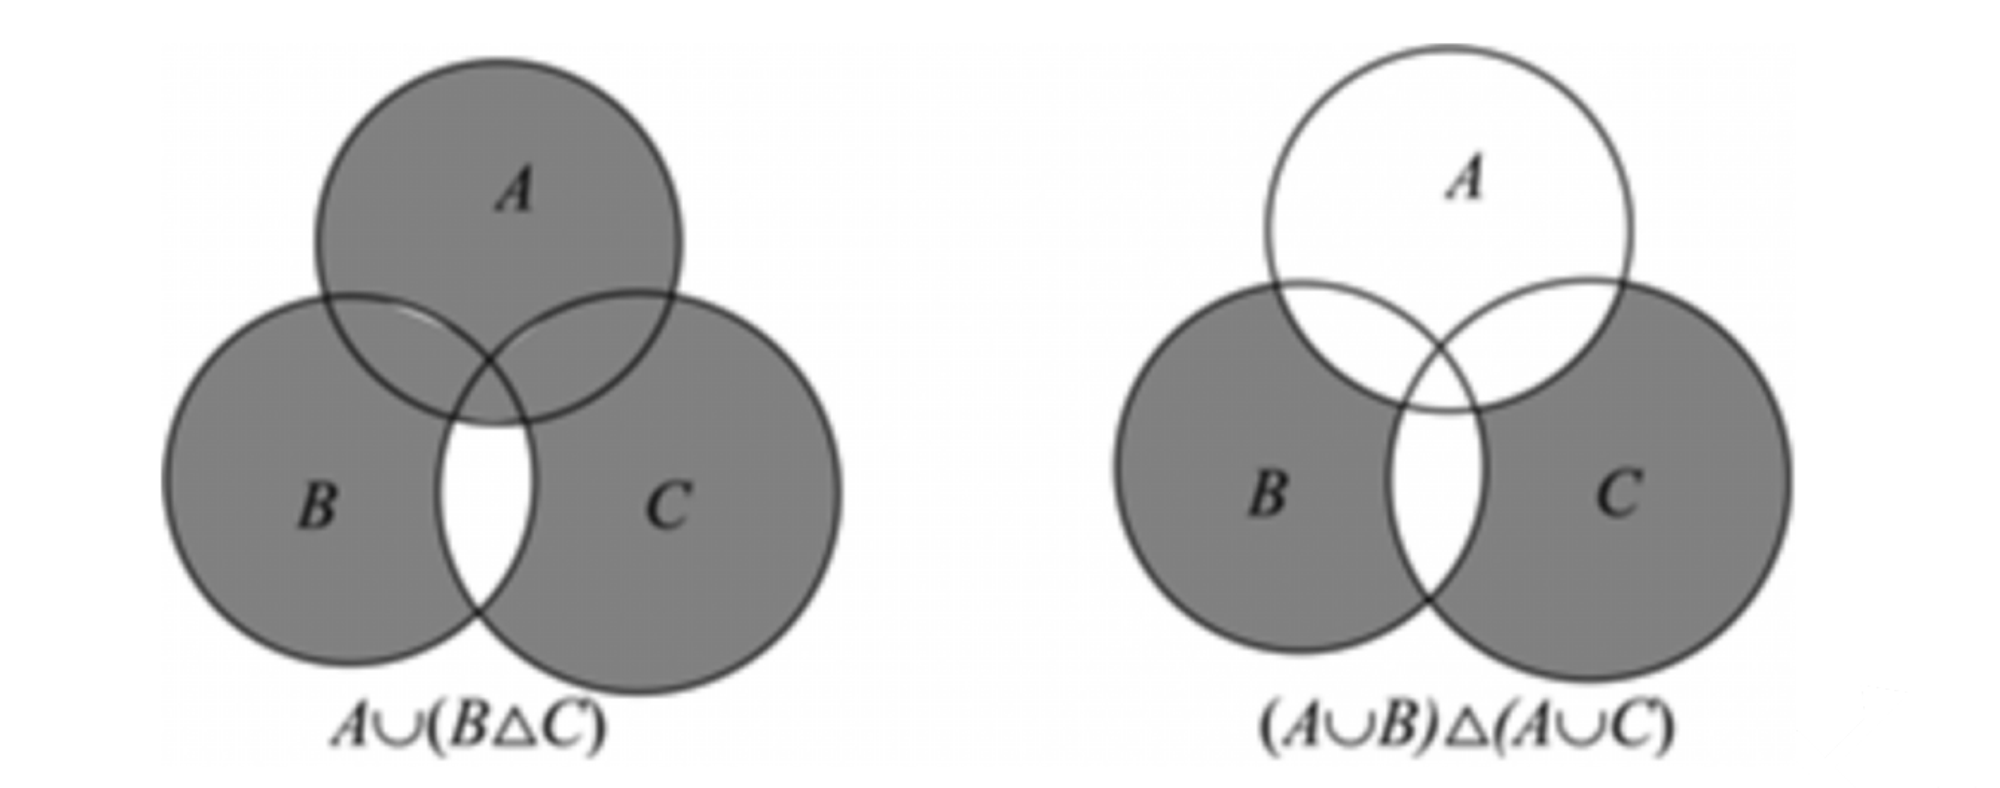
\includegraphics[width=0.85\textwidth]{figures/gao115_q13.png}
\end{center}
\step{所以 $A\cup(B\triangle C)\neq(A\cup B)\triangle(A\cup C)$，④错.}
\step{故选 $C$.}
\solend
\fi

\item 设 $a$、$b$、$c$、$p$ 为实数，若同时满足不等式 $ax^2+bx+c>0$、$bx^2+cx+a>0$ 与 $cx^2+ax+b>0$ 的全体实数 $x$ 所组成的集合等于 $(p,+\infty)$，则关于结论：① $a$、$b$、$c$ 至少有一个为 $0$；② $p=0$. 下列判断中正确的是\mbox{（\quad）}

\keepwithprev
A. ①和②都正确\qquad B. ①和②都错误\qquad C. ①正确，②错误\qquad D. ①错误，②正确

\ifanswer
\solbegin
\step{若同时满足不等式 $ax^2+bx+c>0$、$bx^2+cx+a>0$ 与 $cx^2+ax+b>0$ 的}
\step{全体实数 $x$ 所组成的集合等于 $(p,+\infty)$，必有 $a$,$b$,$c\geqslant0$，}
\step{不妨假设 $a$、$b$、$c$ 没有一个为 $0$，}
\step{则三个不等式均为开口向上的二次函数大于 $0$ 的部分，}
\step{解集的交集应为 $(-\infty,m)\cup(n,+\infty)$ 的形式，矛盾，}
\step{所以 $a$、$b$、$c$ 至少有一个为 $0$，故①正确：}
\step{不妨设 $a=0$，则 $b$,$c\geqslant0$，则不等式组化为 $\begin{cases}bx+c>0\\bx^2+cx>0,\\cx^2+b>0\end{cases}$}
\step{所以 $\begin{cases}x>-\dfrac cb\\x<-\dfrac cb\text{或}x>0\\x\in\R\end{cases}$，取交集得 $(0,+\infty)$，故 $p=0$，故②正确：}
\step{故选 $A$.}
\solend
\fi

\end{enumerate}

\bigsec{三、解答题}

\begin{enumerate}
\setcounter{enumi}{14}

\item 已知 $a>0$，$b>0$，

（1）试比较 $\dfrac{a^2-b^2}{a^2+b^2}$ 与 $\dfrac{a-b}{a+b}$ 的大小；

（2）若 $a+b>4$，求证：$\dfrac a{b+2}$ 和 $\dfrac b{a+2}$ 中至少有一个大于 $\dfrac12$.

\ifanswer
\solbegin
\step{（1）已知 $a>0$，$b>0$，$\dfrac{a^2-b^2}{a^2+b^2}-\dfrac{a-b}{a+b}=\dfrac{2ab(a-b)}{(a^2+b^2)(a+b)}$，}
\step{当 $a>b$ 时，$a-b>0$，所以 $\dfrac{a^2-b^2}{a^2+b^2}-\dfrac{a-b}{a+b}>0$，所以 $\dfrac{a^2-b^2}{a^2+b^2}>\dfrac{a-b}{a+b}$；}
\step{当 $a=b$ 时，$a-b=0$，所以 $\dfrac{a^2-b^2}{a^2+b^2}-\dfrac{a-b}{a+b}=0$，所以 $\dfrac{a^2-b^2}{a^2+b^2}=\dfrac{a-b}{a+b}$；}
\step{当 $a<b$ 时，$a-b<0$，所以 $\dfrac{a^2-b^2}{a^2+b^2}-\dfrac{a-b}{a+b}<0$，所以 $\dfrac{a^2-b^2}{a^2+b^2}<\dfrac{a-b}{a+b}$；}
\step{（2）假设 $\dfrac a{b+2}$ 和 $\dfrac b{a+2}$ 中都不大于 $\dfrac12$，即 $\dfrac b{a+2}\leqslant\dfrac12$，$\dfrac a{b+2}\leqslant\dfrac12$，}
\step{因为 $a>0$，$b>0$，所以 $a+2>0$，$b+2>0$，}
\step{所以 $2b\leqslant a+2$，$2a\leqslant b+2$，}
\step{两式相加得 $2a+2b\leqslant a+2+b+2=a+b+4$，即 $a+b\leqslant4$，}
\step{与已知 $a+b>4$ 矛盾，所以假设错误，}
\step{故 $\dfrac a{b+2}$ 和 $\dfrac b{a+2}$ 中至少有一个大于 $\dfrac12$.}
\solend
\fi

\item 某企业原有 $200$ 名科技人员，年人均工资 $a$ 万元($a>0$). 现加大对某芯片研发力度，该企业把原有 $200$ 名科技人员调整成技术人员和研发人员，其中技术人员 $x$ 名($x\in\N$ 且 $40\leqslant x\leqslant80$). 调整后，研发人员的年人均工资比调整前增加了 $(2x)\%$，技术人员的年人均工资为 $a\left(m-\dfrac x{10}\right)$万元.

（1）若要使调整后研发人员的年总工资不低于调整前 $200$ 名科技人员年总工资的 $1.5$ 倍，求调整后的技术人员最少有多少人？

（2）为了激励研发人员的工作热情和保持技术人员的工作积极性，企业决定在工资方面要同时满足以下两个条件：

①研发人员的年总工资始终不低于技术人员的年总工资；

②技术人员的年人均工资始终不低于调整前 $200$ 名科技人员的年人均工资.

请问是否存在这样的实数 $m$？若存在，求出 $m$ 的范围；若不存在，说明理由.

\ifanswer
\solbegin
\step{（1）由题意得调整后研发人员的年人均工资为 $[1+(2x)\%]a$ 万元，}
\step{那么 $(200-x)[1+(2x)\%]a\geqslant1.5\times200a$ ($a>0$)，}
\step{化简得 $x^2-150x+5000\leqslant0$，解得 $50\leqslant x\leqslant100$，}
\step{由于 $x\in\N$ 且 $40\leqslant x\leqslant80$，因此 $50\leqslant x\leqslant80$，}
\step{因此调整后的技术人员的人数最少为 $50$ 人；}
\step{（2）假设存在实数 $m$，使得技术人员在已知范围内调整后，满足以上两个条件，}
\step{由条件①得 $(200-x)[1+(2x)\%]a\geqslant x\left(m-\dfrac x{10}\right)a$，}
\step{整理得 $m\leqslant\dfrac{200}{x}+\dfrac{2x}{25}+3$；}
\step{因为 $\dfrac{200}{x}+\dfrac{2x}{25}+3\geqslant2\sqrt{\dfrac{200}{x}\cdot\dfrac{2x}{25}}+3=11$，}
\step{当且仅当 $\dfrac{200}{x}=\dfrac{2x}{25}$，即 $x=50$ 时取等号，因此 $m\leqslant11$，}
\step{由条件②得 $a\left(m-\dfrac x{10}\right)\geqslant a$，所以 $m\geqslant\dfrac x{10}+1$；}
\step{又由于 $40\leqslant x\leqslant80$，因此 $m\geqslant9$.}
\step{因此 $m\in[9,11]$.}
\solend
\fi

\item 已知 $a\in\R$，记 $f(x)=ax^2-(a+2)x+2$.

（1）若 $f(x)<3-2x$ 对于一切 $x\in\R$ 恒成立，求实数 $a$ 的取值范围；

（2）求关于 $x$ 不等式 $f(x)\geqslant0$ 的解集；

（3）若存在 $m\in\R$ 使关于 $x$ 的方程 $ax^2-(a+2)\lvert x\rvert+2=\lvert m+2\rvert+\lvert m-1\rvert$ 有四个不同的实根，求实数 $a$ 的取值范围.

\ifanswer
\solbegin
\step{（1）由 $f(x)<3-2x$ 对于一切 $x\in\R$ 恒成立，}
\step{得 $ax^2-ax-1<0$ 对于一切 $x\in\R$ 恒成立，}
\step{当 $a=0$ 时，原式可化为 $-1<0$，恒成立，符合条件；}
\step{当 $a\neq0$ 时，需满足 $\begin{cases}a<0\\\Delta=a^2+4a<0\end{cases}$，解得 $-4<a<0$；}
\step{综上，实数 $a$ 的取值范围是 $(-4,0]$；}
\step{（2）$f(x)\geqslant0$，即 $(ax-2)(x-1)\geqslant0$，}
\step{当 $a=0$ 时，原式化为 $-2x+2\geqslant0$，解集为 $\{x\mid x\leqslant1\}$；}
\step{当 $a>0$ 时，若 $a=2$，原式化为 $2(x-1)^2\geqslant0$，解集为 $\R$；}
\step{若 $0<a<2$，$\dfrac2a>1$，解集为 $\{x\mid x\leqslant1$ 或 $x\geqslant\dfrac2a\}$；}
\step{若 $a>2$，$\dfrac2a<1$，解集为 $\{x\mid x\leqslant\dfrac2a$ 或 $x\geqslant1\}$；}
\step{当 $a<0$ 时，$\dfrac2a<1$，解集为 $\left\{x\,\middle\vert\,\dfrac2a\leqslant x\leqslant1\right\}$；}
\step{综上，当 $a<0$ 时，不等式解集为 $\left\{x\,\middle\vert\,\dfrac2a\leqslant x\leqslant1\right\}$；}
\step{当 $a=0$ 时，不等式解集为 $\{x\mid x\leqslant1\}$；}
\step{当 $0<a<2$ 时，不等式解集为 $\{x\mid x\leqslant1$ 或 $x\geqslant\dfrac2a\}$；}
\step{当 $a=2$ 时，不等式解集为 $\R$；}
\step{当 $a>2$ 时，不等式解集为 $\{x\mid x\leqslant\dfrac2a$ 或 $x\geqslant1\}$；}
\step{（3）由绝对值三角不等式得 $\lvert m+2\rvert+\lvert m-1\rvert\geqslant\lvert(m+2)-(m-1)\rvert=3$，}
\step{即右侧取值范围为 $[3,+\infty)$，}
\step{令 $t=\lvert x\rvert\geqslant0$，原方程转化为 $at^2-(a+2)t+2=k$，$k\in[3,+\infty)$，}
\step{若原方程有四个不同实根，}
\step{需存在 $k\geqslant3$，使得方程 $at^2-(a+2)t+2-k=0$ 有两个不同正实根，}
\step{当 $a\geqslant0$ 时，方程的两根之积为 $\dfrac{2-k}{a}$，}
\step{因为 $k\geqslant3$，所以 $2-k\leqslant-1<0$，两根一正一负，}
\step{最多只有一个正根，对应最多两个 $x$ 根，不符合要求；}
\step{当 $a<0$ 时，两根之积为正，}
\step{要两个根都为正，需要两根之和 $\dfrac{a+2}{a}>0$，解得 $a<-2$，}
\step{再要求存在 $k\geqslant3$ 使得判别式大于 $0$，}
\step{即 $\triangle=(a+2)^2-4a(2-k)>0$ 在 $k\in[3,+\infty)$ 上有解，}
\step{即 $(a-2)^2+4ak>0$ 在 $k\in[3,+\infty)$ 上有解，}
\step{由 $a<0$，得 $(a-2)^2+12a>0$，}
\step{即 $a^2+8a+4>0$，结合 $a<-2$ 解得 $a<-4-2\sqrt3$，}
\step{故实数 $a$ 的取值范围是 $(-\infty,-4-2\sqrt3)$.}
\solend
\fi

\item 设 $A=\{x_1,x_2,\cdots,x_n\}(n\geqslant2,n\in\N)$，且 $x_1,x_2,\cdots,x_n$ 均为正整数，若对于 $A$ 中任意两个元素 $a,b$，当 $a>b$ 时，都有 $\dfrac{b^2}{a-b}\in A$，则称 $A$ 为“$n$ 元好集”.

（1）判断 $\{2,4,6\}$ 是否为“三元好集”，并说明理由；

（2）若集合 $M$ 为“二元好集”，且 $M$ 中所有元素之积小于 $2026$，求所有满足条件的集合 $M$ 的个数；

（3）设 $k\geqslant3,k\in\N$，是否存在“$k$ 元好集”，若存在，求出所有满足条件的“$k$ 元好集”，若不存在，请说明理由.

\ifanswer
\solbegin
\step{（1）取 $a=6,b=2$，则 $\dfrac{b^2}{a-b}=\dfrac44=1\notin\{2,4,6\}$，所以该集合不是三元好集.}
\step{（2）设 $M=\{b,a\}$，其中 $a>b$ 且均为正整数，则 $\dfrac{b^2}{a-b}$ 等于 $a$ 或 $b$.}
\step{若 $\dfrac{b^2}{a-b}=a$，则 $a^2-ab-b^2=0$，从而 $\dfrac ab=\dfrac{1+\sqrt5}{2}$，与 $\dfrac ab$ 为有理数矛盾.}
\step{若 $\dfrac{b^2}{a-b}=b$，则 $a=2b$；}
\step{反之，任意正整数 $b$ 对应的 $\{b,2b\}$ 均为二元好集.}
\step{由元素之积小于 $2026$，得 $2b^2<2026\Leftrightarrow b^2<1013$.}
\step{因为 $31^2=961<1013<1024=32^2$，所以 $b=1,2,\cdots,31$，}
\step{对应 $31$ 个不同的集合.}
\step{（3）假设存在 $k\geqslant3$ 的 $k$ 元好集 $A$，将其元素从小到大排列，}
\step{记最小元素为 $u$，次小元素为 $v$，最大元素为 $w$，则 $0<u<v<w$.}
\step{由 $\dfrac{u^2}{w-u}\in A$，该数不小于 $u$，得 $\dfrac{u^2}{w-u}\geqslant u\Rightarrow w\leqslant2u$.}
\step{又由 $\dfrac{u^2}{v-u}$,$\dfrac{v^2}{w-v}\in A$，这两个数均不超过 $w$，}
\step{得 $\dfrac{u^2}{v-u}\leqslant w$,$\dfrac{v^2}{w-v}\leqslant w$，}
\step{分母均为正，分别去分母后相加，}
\step{得 $u^2+v^2\leqslant w(v-u)+w(w-v)=w(w-u)\leqslant2u^2$，}
\step{于是 $v^2\leqslant u^2$，与 $v>u>0$ 矛盾，所以不存在 $k\geqslant3$ 的 $k$ 元好集.}
\solend
\fi

\end{enumerate}

\end{document}
"
% 紧凑版：xelatex "\def\iscompact{1}% 高一115_复旦附中_10月阶段练习.tex
%   —— 高一上数学“2026-2027 年复旦附中高一上 10 月阶段练习”（试卷版/答案版）
% 试卷版：xelatex 高一115_复旦附中_10月阶段练习.tex
% 答案版：xelatex "\def\isanswer{1}\input{高一115_复旦附中_10月阶段练习.tex}"
% 紧凑版：xelatex "\def\iscompact{1}\input{高一115_复旦附中_10月阶段练习.tex}"
%
% 原始材料：微信公众号“魔都数学加油站”文章，作者破晓，2026-11-06 17:58 发布；
% 连载“27学年高一115”，原文标题“27学年高一115——2026-2027年上海市复旦附中高一上10月阶段练习”；
% 原文链接：https://mp.weixin.qq.com/s/krocP0fMQQ4VM1SQEcLI2Q。
% 正文为 12 张 PNG 页（第 4、6、12 页 2560×3620，其余 4762×6735），
% 题目下印有【解析】或【答案】，为讲评版。
% 题目、解析均据原图转录；卷面红色水印及公众号页脚未录入。
%
% 卷首标题：原卷印作“2026-2027 年复旦附中高一上 10 月阶段练习”（公众号标题中的“上海市”
% 卷面标题行没有，本稿照卷面），年份区间按全稿惯例排 en dash；原卷未印副标题，本稿按题目内容
% 标为“集合与常用逻辑用语、不等式”。
%
% 与原卷的排版差异：
%   ① 原文从第 3 题起，填空题编号为 3—10、选择题为 11—14、解答题为 15—18，共 16 题，
%      本稿保留原题号（与多数卷的 3—21 不同）；
%   ② 原卷每题下直接印【解析】／【答案】，本稿按全稿惯例置于答案版；第 11 题把答案“$B$”
%      印在题干括号内且无【解析】，另提 \ans{}；其余选择题答案在解析末句“故选 …”，括号内留空；
%   ③ 原卷未印副标题，本稿按“知识模块”口径补出；
%   ④ 原卷填空横线按全稿惯例排为 \blankline[4.4em]；选择题括号排 \mbox{（\quad）}、
%      选项段前按惯例加 \keepwithprev；解答题不留作答区（原卷为讲评版，与 109—114 同）；
%   ⑤ 原卷数集排斜体 $R$／$Q$／$N$，按全稿惯例改 \R、\Q、\N。
%
% 判别式与对称差字形：原卷 $\triangle$（等边、扁）与 $\Delta$（等腰、高）两种混用，逐处照录——
%   第 7 题与第 17 题 (3) 的判别式、第 13 题的对称差 $A\triangle B$ 用 \triangle，
%   第 17 题 (1) cases 的判别式用 \Delta。
%
% 子集符号：第 4 题解析的 $(-1,3)\subset(-m,m)$ 印单线（真子集、无下划线），按 18／96
%   成例照录 \subset；第 5 题解析的 $B\subseteq A$ 印有下划线，照录 \subseteq。
%   第 3 题的补集照原卷上划线排 \overline{N}。
%
% 原卷存疑照录：第 9 题解析末行“故可能成立的是①②③”与四种情形的编号一致，照录；
%   第 10 题解析两幅函数图上另有蓝色／红色手写标注（$t$、$t+1$、$s$、$\frac16$ 等），
%   系批改笔迹，随裁图保留、不另作正文录入；第 14 题解析的 cases 三行照原卷排；
%   第 18 题 (2) 解析“所以该集合不是三元好集”前的取例 $a=6,b=2$ 照录。
%
% 行数核对：逐题数 \step/\stepm 条数，合计 133 条（Q3：3；Q4：3；Q5：4；Q6：5；Q7：4；
% Q8：4；Q9：11；Q10：7；Q11：0；Q12：4；Q13：8；Q14：9；Q15：10；Q16：13；
% Q17：32；Q18：16），与原卷印刷行逐题相等（cases 块作一个印刷行计）。第 11 题括号内印
% 答案且无解析，提 \ans{}，不计入 \step 账；第 10、13 题解析内的插图不计入 \step 账。
%
\documentclass[a4paper,11pt]{article}
\usepackage{common}

\begin{document}

\examtitlest[3]{2026--2027 年复旦附中高一上 10 月阶段练习}{集合与常用逻辑用语、不等式}

\bigsec{一、填空题}

\begin{enumerate}
\setcounter{enumi}{2}

\item 已知集合 $M=\{x\mid 4x^2-4x-15>0\}$，$N=\left\{x\,\middle\vert\,\dfrac{x+1}{x-6}>0\right\}$，则 $M\cap\overline{N}=$\blankline[4.4em].

\ifanswer
\solbegin
\step{集合 $M=\{x\mid 4x^2-4x-15>0\}=\{x\mid x>\dfrac52$ 或 $x<-\dfrac32\}$，}
\step{$N=\left\{x\,\middle\vert\,\dfrac{x+1}{x-6}>0\right\}=\{x\mid x>6$ 或 $x<-1\}$，得 $\overline{N}=\{x\mid-1\leqslant x\leqslant6\}$，}
\step{故 $M\cap\overline{N}=\left\{x\,\middle\vert\,\dfrac52<x\leqslant6\right\}$.}
\solend
\fi

\item 已知 $m>0$，不等式 $\lvert x\rvert<m$ 成立的一个充分不必要条件是 $-1<x<3$，则 $m$ 的取值范围是\blankline[4.4em].

\ifanswer
\solbegin
\step{不等式 $-m<x<m$ 成立的一个充分不必要条件是 $-1<x<3$，}
\step{由题意得 $(-1,3)\subset(-m,m)$，则 $m\geqslant3$，此时 $-m\leqslant-3<-1$，}% 原卷印单线 \subset，照录
\step{所以 $m$ 的取值范围是 $\{m\mid m\geqslant3\}$.}
\solend
\fi

\item 已知集合 $A=\{1,2\}$，集合 $B=\{x\mid ax=6\}$，若 $A\cup B=A$，则 $a$ 的所有取值构成的集合为\blankline[4.4em].

\ifanswer
\solbegin
\step{因为 $A\cup B=A$，所以 $B\subseteq A$，}
\step{当 $a=0$ 时，$B=\varnothing$，满足 $B\subseteq A$；}
\step{当 $a\neq0$ 时，$B=\left\{\dfrac6a\right\}$，则 $\dfrac6a=1$ 或 $\dfrac6a=2$，解得 $a=6$ 或 $a=3$，}
\step{综上所述，$a$ 的所有取值构成的集合为 $\{0,3,6\}$.}
\solend
\fi

\item 若关于 $x$ 的不等式 $ax^2+bx+c>0$ 的解集为 $(-3,2)$，则不等式 $ax^2+(a+b)x+c-2a>0$ 的解集为\blankline[4.4em].

\ifanswer
\solbegin
\step{由 $ax^2+bx+c>0$ 的解集为 $(-3,2)$ 得 $a<0$，}
\step{且 $ax^2+bx+c=0$ 时 $x_1=-3$，$x_2=2$，}
\step{得 $-3+2=-\dfrac ba$，即 $b=a$，$-3\times2=\dfrac ca$，即 $c=-6a$，}
\step{代入 $ax^2+(a+b)x+c-2a>0$ 得 $ax^2+2ax-8a>0$ 化简得 $x^2+2x-8<0$，}
\step{解得 $-4<x<2$，故解集为 $(-4,2)$.}
\solend
\fi

\item 已知关于 $x$ 的方程 $x^2-2x+m=0$ 的两个实数根分别为 $x_1$，$x_2$. 若 $x_1^2x_2^2+x_1^2+x_2^2=7$，则实数 $m$ 的值为\blankline[4.4em].

\ifanswer
\solbegin
\step{由韦达定理得 $x_1+x_2=2$，$x_1x_2=m$，}
\step{$x_1^2x_2^2+x_1^2+x_2^2=(x_1x_2)^2+(x_1+x_2)^2-2x_1x_2=m^2+4-2m$，}
\step{由 $m^2+4-2m=7$，得 $m^2-2m-3=0$，解得 $m=3$ 或 $m=-1$，}
\step{方程有两个实数根，故 $\triangle=4-4m\geqslant0$，即 $m\leqslant1$，所以 $m=-1$.}
\solend
\fi

\item 已知 $x>1$，若 $x^2-xy+y=0$，则 $x+y$ 的最小值是\blankline[4.4em].

\ifanswer
\solbegin
\step{由于 $x^2-xy+y=0$，则 $y=\dfrac{x^2}{x-1}>0$，}
\step{则 $x+y=x+\dfrac{x^2}{x-1}=\dfrac{2x^2-x}{x-1}=\dfrac{2(x-1)^2+3(x-1)+1}{x-1}$}
\step{$=2(x-1)+\dfrac1{x-1}+3\geqslant2\sqrt{2(x-1)\cdot\dfrac1{x-1}}+3=2\sqrt2+3$，}
\step{当且仅当 $x=1+\dfrac{\sqrt2}{2}$ 时取等号，故最小值是 $2\sqrt2+3$.}
\solend
\fi

\item 若集合 $A=B_1\cup B_2\cup\cdots\cup B_n$，其中 $B_1$、$B_2$、$\cdots$、$B_n$ 为非空集合，$B_i\cap B_j=\varnothing$，$1\leqslant i<j\leqslant n$，则称集合 $\{B_1,B_2,\cdots,B_n\}$ 为集合 $A$ 的一个 $n$ 划分. 例如：集合 $\{\{1,2\},\{3\}\}$，$\{\{1,3\},\{2\}\}$，$\{\{2,3\},\{1\}\}$ 均为集合 $\{1,2,3\}$ 的一个 $2$ 划分. 设 $\{B_1,B_2\}$ 为有理数集 $\Q$ 的一个 $2$ 划分，且满足对任意 $x\in B_1$，任意 $y\in B_2$，都有 $x<y$. 则对于 $B_1$、$B_2$ 有：

① $B_1$ 中的元素存在最大值，$B_2$ 中的元素不存在最小值；

② $B_1$ 中的元素不存在最大值，$B_2$ 中的元素存在最小值；

③ $B_1$ 中的元素不存在最大值，$B_2$ 中的元素不存在最小值；

④ $B_1$ 中的元素存在最大值，$B_2$ 中的元素存在最小值；

对于以上四种情况，可能成立的序号有\blankline[4.4em].

\ifanswer
\solbegin
\step{对于①，$B_1=\{x\in\Q\mid x\leqslant2\}$，$B_2=\{x\in\Q\mid x>2\}$，①可能成立；}
\step{对于②，$B_1=\{x\in\Q\mid x<2\}$，$B_2=\{x\in\Q\mid x\geqslant2\}$，②可能成立；}
\step{对于③，$B_1=\{x\in\Q\mid x<\pi\}$，$B_2=\{x\in\Q\mid x>\pi\}$，③可能成立；}
\step{对于④，假设④成立，}
\step{不妨设 $B_1$ 中的元素的最大值为 $s$，$B_2$ 中的元素的最小值为 $t$，}
\step{由题意得 $s<t$，所以 $s<\dfrac{s+t}{2}<t$，}
\step{因为 $s$ 为 $B_1$ 中的元素的最大值，所以 $\dfrac{s+t}{2}\notin B_1$，}
\step{因为 $t$ 为 $B_2$ 中的元素的最小值，所以 $\dfrac{s+t}{2}\notin B_2$，}
\step{又 $B_1\cup B_2=\Q$，所以 $\dfrac{s+t}{2}\notin\Q$，与 $\dfrac{s+t}{2}\in\Q$ 矛盾，}
\step{所以假设不成立，即④不可能成立.}
\step{故可能成立的是①②③.}
\solend
\fi

\item 已知集合 $A=\left[s,s+\dfrac16\right]\cup[t,t+1]$，其中 $1\notin A$ 且 $s+\dfrac16<t$，函数 $f(x)=\dfrac x{x-1}$，且对任意 $a\in A$，都有 $f(a)\in A$，则 $t$ 的值是\blankline[4.4em].

\ifanswer
\solbegin
\step{若 $\left[s,s+\dfrac16\right]$,$[t,t+1]$ 在 $f(x)=\dfrac x{x-1}$ 图像的同侧，}
\step{则点 $\left(t,s+\dfrac16\right)$,$(t+1,s)$ 在 $f(x)=\dfrac x{x-1}$ 的图像上，}
\step{所以 $\dfrac t{t-1}=\dfrac{t+1}{t}+\dfrac16$，解得 $t=-2$ 或 $t=3$，检验得 $t=3$；}
\step{若 $\left[s,s+\dfrac16\right]$,$[t,t+1]$ 在 $f(x)=\dfrac x{x-1}$ 图像的两侧，}
\step{则点 $(t,t+1)$ 在 $f(x)=\dfrac x{x-1}$ 的图像上，}
\step{所以 $t+1=\dfrac t{t-1}$，解得 $t=\dfrac{1\pm\sqrt5}{2}$，检验得 $t=\dfrac{1+\sqrt5}{2}$，}
\step{综上，$t=\dfrac{1+\sqrt5}{2}$ 或 $t=3$.}
\begin{center}
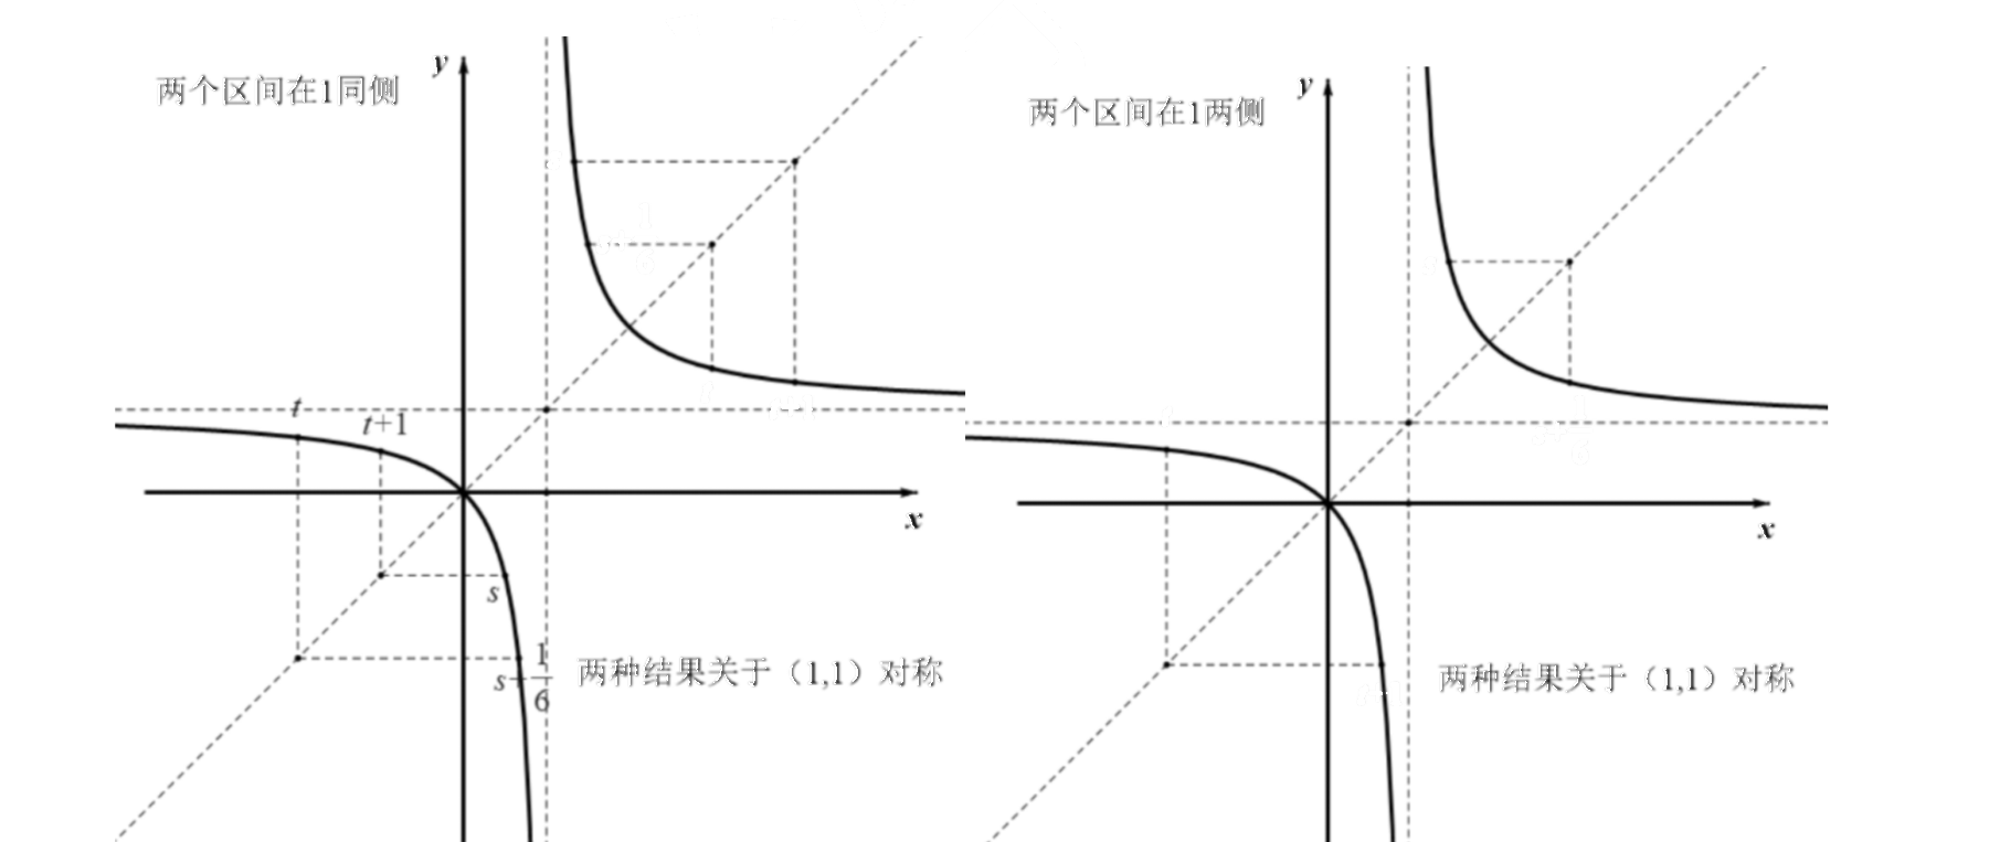
\includegraphics[width=0.92\textwidth]{figures/gao115_q10.png}
\end{center}
\solend
\fi

\end{enumerate}

\bigsec{二、选择题}

\begin{enumerate}
\setcounter{enumi}{10}

\item “对任意有理数 $x$ 都有 $x^2\neq2$”的否定形式是\mbox{（\quad）}% 原卷把答案“$B$”印在题干括号内、无【解析】

\keepwithprev
A. 存在有理数 $x$ 使得 $x^2\neq2$\qquad\qquad B. 存在有理数 $x$ 使得 $x^2=2$

C. 存在无理数 $x$ 使得 $x^2\neq2$\qquad\qquad D. 存在无理数 $x$ 使得 $x^2=2$

\ifanswer
\ans{$B$}
\fi

\item 已知 $a$、$b$ 都是实数，那么“$a^3>b^3$”是“$a^2>b^2$”的\mbox{（\quad）}

\keepwithprev
A. 充分不必要条件\qquad\qquad B. 必要不充分条件

C. 充要条件\qquad\qquad\qquad D. 既不充分也不必要条件

\ifanswer
\solbegin
\step{因为 $a^3>b^3$ 等价于 $a>b$，}
\step{由于 $a$、$b$ 正负不定，所以由 $a>b$ 不能得到 $a^2>b^2$，}
\step{由 $a^2>b^2$ 也不能得到 $a>b$，}
\step{因此“$a^3>b^3$”是“$a^2>b^2$”的既不充分也不必要条件. 故选 $D$.}
\solend
\fi

\item 定义集合运算 $A-B=\{x\mid x\in A$ 且 $x\notin B\}$，将 $A\triangle B=(A-B)\cup(B-A)$ 称为集合 $A$ 与集合 $B$ 的对称差.

命题一：$A\triangle B=B\triangle A$；

命题二：$A\triangle\varnothing=A$；

命题三：$A\cap(B\triangle C)=(A\cap B)\triangle(A\cap C)$；

命题四：$A\cup(B\triangle C)=(A\cup B)\triangle(A\cup C)$；

其中正确命题的个数是\mbox{（\quad）}

\keepwithprev
A. $1$\qquad\qquad B. $2$\qquad\qquad C. $3$\qquad\qquad D. $4$

\ifanswer
\solbegin
\step{对于①，$B\triangle A=(B-A)\cup(A-B)=(A-B)\cup(B-A)=A\triangle B$，①对；}
\step{对于②，$A-B=\{x\mid x\in A$ 且 $x\notin B\}=\{x\mid x\in A$ 且 $x\notin(A\cap B)\}$}
\step{$=A-(A\cap B)$，则 $A\triangle\varnothing=(A-\varnothing)\cup(\varnothing-A)=A\cup\varnothing=A$，②对；}
\step{对于③，$A\cap(B\triangle C)=A\cap(B\cup C-B\cap C)=A\cap(B\cup C)-A\cap(B\cap C)$}
\step{$=(A\cap B)\cup(A\cap C)-(A\cap B)\cap(A\cap C)=(A\cap B)\triangle(A\cap C)$，③对；}
\step{对于④，如图所示：}
\begin{center}
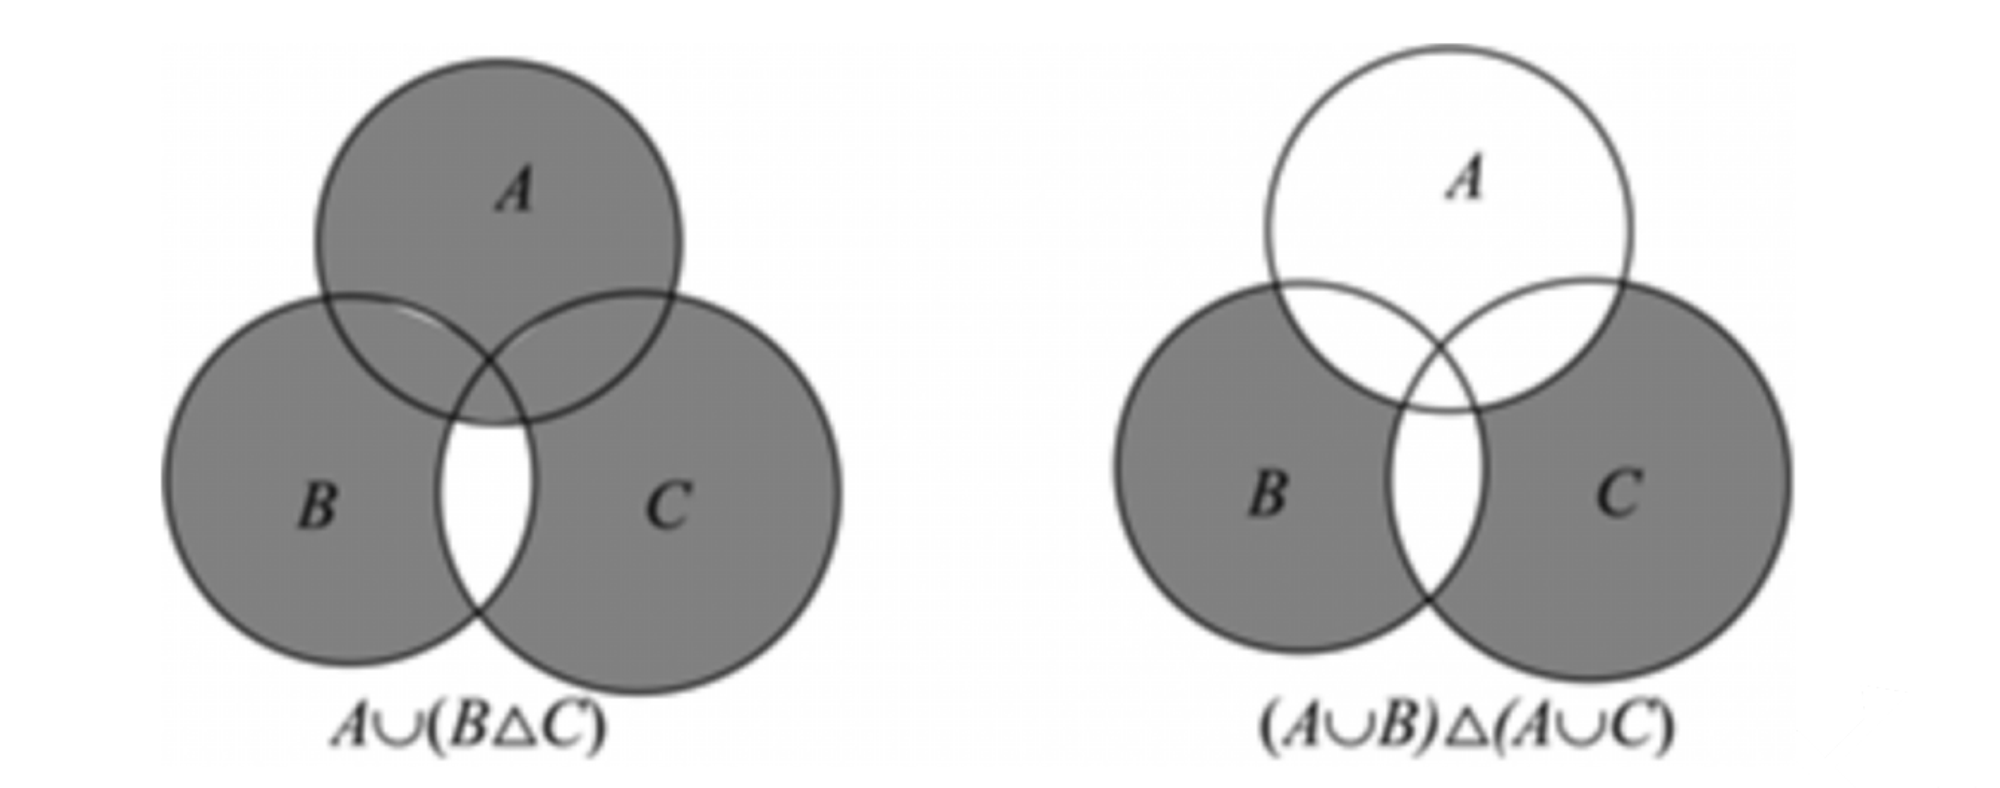
\includegraphics[width=0.85\textwidth]{figures/gao115_q13.png}
\end{center}
\step{所以 $A\cup(B\triangle C)\neq(A\cup B)\triangle(A\cup C)$，④错.}
\step{故选 $C$.}
\solend
\fi

\item 设 $a$、$b$、$c$、$p$ 为实数，若同时满足不等式 $ax^2+bx+c>0$、$bx^2+cx+a>0$ 与 $cx^2+ax+b>0$ 的全体实数 $x$ 所组成的集合等于 $(p,+\infty)$，则关于结论：① $a$、$b$、$c$ 至少有一个为 $0$；② $p=0$. 下列判断中正确的是\mbox{（\quad）}

\keepwithprev
A. ①和②都正确\qquad B. ①和②都错误\qquad C. ①正确，②错误\qquad D. ①错误，②正确

\ifanswer
\solbegin
\step{若同时满足不等式 $ax^2+bx+c>0$、$bx^2+cx+a>0$ 与 $cx^2+ax+b>0$ 的}
\step{全体实数 $x$ 所组成的集合等于 $(p,+\infty)$，必有 $a$,$b$,$c\geqslant0$，}
\step{不妨假设 $a$、$b$、$c$ 没有一个为 $0$，}
\step{则三个不等式均为开口向上的二次函数大于 $0$ 的部分，}
\step{解集的交集应为 $(-\infty,m)\cup(n,+\infty)$ 的形式，矛盾，}
\step{所以 $a$、$b$、$c$ 至少有一个为 $0$，故①正确：}
\step{不妨设 $a=0$，则 $b$,$c\geqslant0$，则不等式组化为 $\begin{cases}bx+c>0\\bx^2+cx>0,\\cx^2+b>0\end{cases}$}
\step{所以 $\begin{cases}x>-\dfrac cb\\x<-\dfrac cb\text{或}x>0\\x\in\R\end{cases}$，取交集得 $(0,+\infty)$，故 $p=0$，故②正确：}
\step{故选 $A$.}
\solend
\fi

\end{enumerate}

\bigsec{三、解答题}

\begin{enumerate}
\setcounter{enumi}{14}

\item 已知 $a>0$，$b>0$，

（1）试比较 $\dfrac{a^2-b^2}{a^2+b^2}$ 与 $\dfrac{a-b}{a+b}$ 的大小；

（2）若 $a+b>4$，求证：$\dfrac a{b+2}$ 和 $\dfrac b{a+2}$ 中至少有一个大于 $\dfrac12$.

\ifanswer
\solbegin
\step{（1）已知 $a>0$，$b>0$，$\dfrac{a^2-b^2}{a^2+b^2}-\dfrac{a-b}{a+b}=\dfrac{2ab(a-b)}{(a^2+b^2)(a+b)}$，}
\step{当 $a>b$ 时，$a-b>0$，所以 $\dfrac{a^2-b^2}{a^2+b^2}-\dfrac{a-b}{a+b}>0$，所以 $\dfrac{a^2-b^2}{a^2+b^2}>\dfrac{a-b}{a+b}$；}
\step{当 $a=b$ 时，$a-b=0$，所以 $\dfrac{a^2-b^2}{a^2+b^2}-\dfrac{a-b}{a+b}=0$，所以 $\dfrac{a^2-b^2}{a^2+b^2}=\dfrac{a-b}{a+b}$；}
\step{当 $a<b$ 时，$a-b<0$，所以 $\dfrac{a^2-b^2}{a^2+b^2}-\dfrac{a-b}{a+b}<0$，所以 $\dfrac{a^2-b^2}{a^2+b^2}<\dfrac{a-b}{a+b}$；}
\step{（2）假设 $\dfrac a{b+2}$ 和 $\dfrac b{a+2}$ 中都不大于 $\dfrac12$，即 $\dfrac b{a+2}\leqslant\dfrac12$，$\dfrac a{b+2}\leqslant\dfrac12$，}
\step{因为 $a>0$，$b>0$，所以 $a+2>0$，$b+2>0$，}
\step{所以 $2b\leqslant a+2$，$2a\leqslant b+2$，}
\step{两式相加得 $2a+2b\leqslant a+2+b+2=a+b+4$，即 $a+b\leqslant4$，}
\step{与已知 $a+b>4$ 矛盾，所以假设错误，}
\step{故 $\dfrac a{b+2}$ 和 $\dfrac b{a+2}$ 中至少有一个大于 $\dfrac12$.}
\solend
\fi

\item 某企业原有 $200$ 名科技人员，年人均工资 $a$ 万元($a>0$). 现加大对某芯片研发力度，该企业把原有 $200$ 名科技人员调整成技术人员和研发人员，其中技术人员 $x$ 名($x\in\N$ 且 $40\leqslant x\leqslant80$). 调整后，研发人员的年人均工资比调整前增加了 $(2x)\%$，技术人员的年人均工资为 $a\left(m-\dfrac x{10}\right)$万元.

（1）若要使调整后研发人员的年总工资不低于调整前 $200$ 名科技人员年总工资的 $1.5$ 倍，求调整后的技术人员最少有多少人？

（2）为了激励研发人员的工作热情和保持技术人员的工作积极性，企业决定在工资方面要同时满足以下两个条件：

①研发人员的年总工资始终不低于技术人员的年总工资；

②技术人员的年人均工资始终不低于调整前 $200$ 名科技人员的年人均工资.

请问是否存在这样的实数 $m$？若存在，求出 $m$ 的范围；若不存在，说明理由.

\ifanswer
\solbegin
\step{（1）由题意得调整后研发人员的年人均工资为 $[1+(2x)\%]a$ 万元，}
\step{那么 $(200-x)[1+(2x)\%]a\geqslant1.5\times200a$ ($a>0$)，}
\step{化简得 $x^2-150x+5000\leqslant0$，解得 $50\leqslant x\leqslant100$，}
\step{由于 $x\in\N$ 且 $40\leqslant x\leqslant80$，因此 $50\leqslant x\leqslant80$，}
\step{因此调整后的技术人员的人数最少为 $50$ 人；}
\step{（2）假设存在实数 $m$，使得技术人员在已知范围内调整后，满足以上两个条件，}
\step{由条件①得 $(200-x)[1+(2x)\%]a\geqslant x\left(m-\dfrac x{10}\right)a$，}
\step{整理得 $m\leqslant\dfrac{200}{x}+\dfrac{2x}{25}+3$；}
\step{因为 $\dfrac{200}{x}+\dfrac{2x}{25}+3\geqslant2\sqrt{\dfrac{200}{x}\cdot\dfrac{2x}{25}}+3=11$，}
\step{当且仅当 $\dfrac{200}{x}=\dfrac{2x}{25}$，即 $x=50$ 时取等号，因此 $m\leqslant11$，}
\step{由条件②得 $a\left(m-\dfrac x{10}\right)\geqslant a$，所以 $m\geqslant\dfrac x{10}+1$；}
\step{又由于 $40\leqslant x\leqslant80$，因此 $m\geqslant9$.}
\step{因此 $m\in[9,11]$.}
\solend
\fi

\item 已知 $a\in\R$，记 $f(x)=ax^2-(a+2)x+2$.

（1）若 $f(x)<3-2x$ 对于一切 $x\in\R$ 恒成立，求实数 $a$ 的取值范围；

（2）求关于 $x$ 不等式 $f(x)\geqslant0$ 的解集；

（3）若存在 $m\in\R$ 使关于 $x$ 的方程 $ax^2-(a+2)\lvert x\rvert+2=\lvert m+2\rvert+\lvert m-1\rvert$ 有四个不同的实根，求实数 $a$ 的取值范围.

\ifanswer
\solbegin
\step{（1）由 $f(x)<3-2x$ 对于一切 $x\in\R$ 恒成立，}
\step{得 $ax^2-ax-1<0$ 对于一切 $x\in\R$ 恒成立，}
\step{当 $a=0$ 时，原式可化为 $-1<0$，恒成立，符合条件；}
\step{当 $a\neq0$ 时，需满足 $\begin{cases}a<0\\\Delta=a^2+4a<0\end{cases}$，解得 $-4<a<0$；}
\step{综上，实数 $a$ 的取值范围是 $(-4,0]$；}
\step{（2）$f(x)\geqslant0$，即 $(ax-2)(x-1)\geqslant0$，}
\step{当 $a=0$ 时，原式化为 $-2x+2\geqslant0$，解集为 $\{x\mid x\leqslant1\}$；}
\step{当 $a>0$ 时，若 $a=2$，原式化为 $2(x-1)^2\geqslant0$，解集为 $\R$；}
\step{若 $0<a<2$，$\dfrac2a>1$，解集为 $\{x\mid x\leqslant1$ 或 $x\geqslant\dfrac2a\}$；}
\step{若 $a>2$，$\dfrac2a<1$，解集为 $\{x\mid x\leqslant\dfrac2a$ 或 $x\geqslant1\}$；}
\step{当 $a<0$ 时，$\dfrac2a<1$，解集为 $\left\{x\,\middle\vert\,\dfrac2a\leqslant x\leqslant1\right\}$；}
\step{综上，当 $a<0$ 时，不等式解集为 $\left\{x\,\middle\vert\,\dfrac2a\leqslant x\leqslant1\right\}$；}
\step{当 $a=0$ 时，不等式解集为 $\{x\mid x\leqslant1\}$；}
\step{当 $0<a<2$ 时，不等式解集为 $\{x\mid x\leqslant1$ 或 $x\geqslant\dfrac2a\}$；}
\step{当 $a=2$ 时，不等式解集为 $\R$；}
\step{当 $a>2$ 时，不等式解集为 $\{x\mid x\leqslant\dfrac2a$ 或 $x\geqslant1\}$；}
\step{（3）由绝对值三角不等式得 $\lvert m+2\rvert+\lvert m-1\rvert\geqslant\lvert(m+2)-(m-1)\rvert=3$，}
\step{即右侧取值范围为 $[3,+\infty)$，}
\step{令 $t=\lvert x\rvert\geqslant0$，原方程转化为 $at^2-(a+2)t+2=k$，$k\in[3,+\infty)$，}
\step{若原方程有四个不同实根，}
\step{需存在 $k\geqslant3$，使得方程 $at^2-(a+2)t+2-k=0$ 有两个不同正实根，}
\step{当 $a\geqslant0$ 时，方程的两根之积为 $\dfrac{2-k}{a}$，}
\step{因为 $k\geqslant3$，所以 $2-k\leqslant-1<0$，两根一正一负，}
\step{最多只有一个正根，对应最多两个 $x$ 根，不符合要求；}
\step{当 $a<0$ 时，两根之积为正，}
\step{要两个根都为正，需要两根之和 $\dfrac{a+2}{a}>0$，解得 $a<-2$，}
\step{再要求存在 $k\geqslant3$ 使得判别式大于 $0$，}
\step{即 $\triangle=(a+2)^2-4a(2-k)>0$ 在 $k\in[3,+\infty)$ 上有解，}
\step{即 $(a-2)^2+4ak>0$ 在 $k\in[3,+\infty)$ 上有解，}
\step{由 $a<0$，得 $(a-2)^2+12a>0$，}
\step{即 $a^2+8a+4>0$，结合 $a<-2$ 解得 $a<-4-2\sqrt3$，}
\step{故实数 $a$ 的取值范围是 $(-\infty,-4-2\sqrt3)$.}
\solend
\fi

\item 设 $A=\{x_1,x_2,\cdots,x_n\}(n\geqslant2,n\in\N)$，且 $x_1,x_2,\cdots,x_n$ 均为正整数，若对于 $A$ 中任意两个元素 $a,b$，当 $a>b$ 时，都有 $\dfrac{b^2}{a-b}\in A$，则称 $A$ 为“$n$ 元好集”.

（1）判断 $\{2,4,6\}$ 是否为“三元好集”，并说明理由；

（2）若集合 $M$ 为“二元好集”，且 $M$ 中所有元素之积小于 $2026$，求所有满足条件的集合 $M$ 的个数；

（3）设 $k\geqslant3,k\in\N$，是否存在“$k$ 元好集”，若存在，求出所有满足条件的“$k$ 元好集”，若不存在，请说明理由.

\ifanswer
\solbegin
\step{（1）取 $a=6,b=2$，则 $\dfrac{b^2}{a-b}=\dfrac44=1\notin\{2,4,6\}$，所以该集合不是三元好集.}
\step{（2）设 $M=\{b,a\}$，其中 $a>b$ 且均为正整数，则 $\dfrac{b^2}{a-b}$ 等于 $a$ 或 $b$.}
\step{若 $\dfrac{b^2}{a-b}=a$，则 $a^2-ab-b^2=0$，从而 $\dfrac ab=\dfrac{1+\sqrt5}{2}$，与 $\dfrac ab$ 为有理数矛盾.}
\step{若 $\dfrac{b^2}{a-b}=b$，则 $a=2b$；}
\step{反之，任意正整数 $b$ 对应的 $\{b,2b\}$ 均为二元好集.}
\step{由元素之积小于 $2026$，得 $2b^2<2026\Leftrightarrow b^2<1013$.}
\step{因为 $31^2=961<1013<1024=32^2$，所以 $b=1,2,\cdots,31$，}
\step{对应 $31$ 个不同的集合.}
\step{（3）假设存在 $k\geqslant3$ 的 $k$ 元好集 $A$，将其元素从小到大排列，}
\step{记最小元素为 $u$，次小元素为 $v$，最大元素为 $w$，则 $0<u<v<w$.}
\step{由 $\dfrac{u^2}{w-u}\in A$，该数不小于 $u$，得 $\dfrac{u^2}{w-u}\geqslant u\Rightarrow w\leqslant2u$.}
\step{又由 $\dfrac{u^2}{v-u}$,$\dfrac{v^2}{w-v}\in A$，这两个数均不超过 $w$，}
\step{得 $\dfrac{u^2}{v-u}\leqslant w$,$\dfrac{v^2}{w-v}\leqslant w$，}
\step{分母均为正，分别去分母后相加，}
\step{得 $u^2+v^2\leqslant w(v-u)+w(w-v)=w(w-u)\leqslant2u^2$，}
\step{于是 $v^2\leqslant u^2$，与 $v>u>0$ 矛盾，所以不存在 $k\geqslant3$ 的 $k$ 元好集.}
\solend
\fi

\end{enumerate}

\end{document}
"
%
% 原始材料：微信公众号“魔都数学加油站”文章，作者破晓，2026-11-06 17:58 发布；
% 连载“27学年高一115”，原文标题“27学年高一115——2026-2027年上海市复旦附中高一上10月阶段练习”；
% 原文链接：https://mp.weixin.qq.com/s/krocP0fMQQ4VM1SQEcLI2Q。
% 正文为 12 张 PNG 页（第 4、6、12 页 2560×3620，其余 4762×6735），
% 题目下印有【解析】或【答案】，为讲评版。
% 题目、解析均据原图转录；卷面红色水印及公众号页脚未录入。
%
% 卷首标题：原卷印作“2026-2027 年复旦附中高一上 10 月阶段练习”（公众号标题中的“上海市”
% 卷面标题行没有，本稿照卷面），年份区间按全稿惯例排 en dash；原卷未印副标题，本稿按题目内容
% 标为“集合与常用逻辑用语、不等式”。
%
% 与原卷的排版差异：
%   ① 原文从第 3 题起，填空题编号为 3—10、选择题为 11—14、解答题为 15—18，共 16 题，
%      本稿保留原题号（与多数卷的 3—21 不同）；
%   ② 原卷每题下直接印【解析】／【答案】，本稿按全稿惯例置于答案版；第 11 题把答案“$B$”
%      印在题干括号内且无【解析】，另提 \ans{}；其余选择题答案在解析末句“故选 …”，括号内留空；
%   ③ 原卷未印副标题，本稿按“知识模块”口径补出；
%   ④ 原卷填空横线按全稿惯例排为 \blankline[4.4em]；选择题括号排 \mbox{（\quad）}、
%      选项段前按惯例加 \keepwithprev；解答题不留作答区（原卷为讲评版，与 109—114 同）；
%   ⑤ 原卷数集排斜体 $R$／$Q$／$N$，按全稿惯例改 \R、\Q、\N。
%
% 判别式与对称差字形：原卷 $\triangle$（等边、扁）与 $\Delta$（等腰、高）两种混用，逐处照录——
%   第 7 题与第 17 题 (3) 的判别式、第 13 题的对称差 $A\triangle B$ 用 \triangle，
%   第 17 题 (1) cases 的判别式用 \Delta。
%
% 子集符号：第 4 题解析的 $(-1,3)\subset(-m,m)$ 印单线（真子集、无下划线），按 18／96
%   成例照录 \subset；第 5 题解析的 $B\subseteq A$ 印有下划线，照录 \subseteq。
%   第 3 题的补集照原卷上划线排 \overline{N}。
%
% 原卷存疑照录：第 9 题解析末行“故可能成立的是①②③”与四种情形的编号一致，照录；
%   第 10 题解析两幅函数图上另有蓝色／红色手写标注（$t$、$t+1$、$s$、$\frac16$ 等），
%   系批改笔迹，随裁图保留、不另作正文录入；第 14 题解析的 cases 三行照原卷排；
%   第 18 题 (2) 解析“所以该集合不是三元好集”前的取例 $a=6,b=2$ 照录。
%
% 行数核对：逐题数 \step/\stepm 条数，合计 133 条（Q3：3；Q4：3；Q5：4；Q6：5；Q7：4；
% Q8：4；Q9：11；Q10：7；Q11：0；Q12：4；Q13：8；Q14：9；Q15：10；Q16：13；
% Q17：32；Q18：16），与原卷印刷行逐题相等（cases 块作一个印刷行计）。第 11 题括号内印
% 答案且无解析，提 \ans{}，不计入 \step 账；第 10、13 题解析内的插图不计入 \step 账。
%
\documentclass[a4paper,11pt]{article}
\usepackage{common}

\begin{document}

\examtitlest[3]{2026--2027 年复旦附中高一上 10 月阶段练习}{集合与常用逻辑用语、不等式}

\bigsec{一、填空题}

\begin{enumerate}
\setcounter{enumi}{2}

\item 已知集合 $M=\{x\mid 4x^2-4x-15>0\}$，$N=\left\{x\,\middle\vert\,\dfrac{x+1}{x-6}>0\right\}$，则 $M\cap\overline{N}=$\blankline[4.4em].

\ifanswer
\solbegin
\step{集合 $M=\{x\mid 4x^2-4x-15>0\}=\{x\mid x>\dfrac52$ 或 $x<-\dfrac32\}$，}
\step{$N=\left\{x\,\middle\vert\,\dfrac{x+1}{x-6}>0\right\}=\{x\mid x>6$ 或 $x<-1\}$，得 $\overline{N}=\{x\mid-1\leqslant x\leqslant6\}$，}
\step{故 $M\cap\overline{N}=\left\{x\,\middle\vert\,\dfrac52<x\leqslant6\right\}$.}
\solend
\fi

\item 已知 $m>0$，不等式 $\lvert x\rvert<m$ 成立的一个充分不必要条件是 $-1<x<3$，则 $m$ 的取值范围是\blankline[4.4em].

\ifanswer
\solbegin
\step{不等式 $-m<x<m$ 成立的一个充分不必要条件是 $-1<x<3$，}
\step{由题意得 $(-1,3)\subset(-m,m)$，则 $m\geqslant3$，此时 $-m\leqslant-3<-1$，}% 原卷印单线 \subset，照录
\step{所以 $m$ 的取值范围是 $\{m\mid m\geqslant3\}$.}
\solend
\fi

\item 已知集合 $A=\{1,2\}$，集合 $B=\{x\mid ax=6\}$，若 $A\cup B=A$，则 $a$ 的所有取值构成的集合为\blankline[4.4em].

\ifanswer
\solbegin
\step{因为 $A\cup B=A$，所以 $B\subseteq A$，}
\step{当 $a=0$ 时，$B=\varnothing$，满足 $B\subseteq A$；}
\step{当 $a\neq0$ 时，$B=\left\{\dfrac6a\right\}$，则 $\dfrac6a=1$ 或 $\dfrac6a=2$，解得 $a=6$ 或 $a=3$，}
\step{综上所述，$a$ 的所有取值构成的集合为 $\{0,3,6\}$.}
\solend
\fi

\item 若关于 $x$ 的不等式 $ax^2+bx+c>0$ 的解集为 $(-3,2)$，则不等式 $ax^2+(a+b)x+c-2a>0$ 的解集为\blankline[4.4em].

\ifanswer
\solbegin
\step{由 $ax^2+bx+c>0$ 的解集为 $(-3,2)$ 得 $a<0$，}
\step{且 $ax^2+bx+c=0$ 时 $x_1=-3$，$x_2=2$，}
\step{得 $-3+2=-\dfrac ba$，即 $b=a$，$-3\times2=\dfrac ca$，即 $c=-6a$，}
\step{代入 $ax^2+(a+b)x+c-2a>0$ 得 $ax^2+2ax-8a>0$ 化简得 $x^2+2x-8<0$，}
\step{解得 $-4<x<2$，故解集为 $(-4,2)$.}
\solend
\fi

\item 已知关于 $x$ 的方程 $x^2-2x+m=0$ 的两个实数根分别为 $x_1$，$x_2$. 若 $x_1^2x_2^2+x_1^2+x_2^2=7$，则实数 $m$ 的值为\blankline[4.4em].

\ifanswer
\solbegin
\step{由韦达定理得 $x_1+x_2=2$，$x_1x_2=m$，}
\step{$x_1^2x_2^2+x_1^2+x_2^2=(x_1x_2)^2+(x_1+x_2)^2-2x_1x_2=m^2+4-2m$，}
\step{由 $m^2+4-2m=7$，得 $m^2-2m-3=0$，解得 $m=3$ 或 $m=-1$，}
\step{方程有两个实数根，故 $\triangle=4-4m\geqslant0$，即 $m\leqslant1$，所以 $m=-1$.}
\solend
\fi

\item 已知 $x>1$，若 $x^2-xy+y=0$，则 $x+y$ 的最小值是\blankline[4.4em].

\ifanswer
\solbegin
\step{由于 $x^2-xy+y=0$，则 $y=\dfrac{x^2}{x-1}>0$，}
\step{则 $x+y=x+\dfrac{x^2}{x-1}=\dfrac{2x^2-x}{x-1}=\dfrac{2(x-1)^2+3(x-1)+1}{x-1}$}
\step{$=2(x-1)+\dfrac1{x-1}+3\geqslant2\sqrt{2(x-1)\cdot\dfrac1{x-1}}+3=2\sqrt2+3$，}
\step{当且仅当 $x=1+\dfrac{\sqrt2}{2}$ 时取等号，故最小值是 $2\sqrt2+3$.}
\solend
\fi

\item 若集合 $A=B_1\cup B_2\cup\cdots\cup B_n$，其中 $B_1$、$B_2$、$\cdots$、$B_n$ 为非空集合，$B_i\cap B_j=\varnothing$，$1\leqslant i<j\leqslant n$，则称集合 $\{B_1,B_2,\cdots,B_n\}$ 为集合 $A$ 的一个 $n$ 划分. 例如：集合 $\{\{1,2\},\{3\}\}$，$\{\{1,3\},\{2\}\}$，$\{\{2,3\},\{1\}\}$ 均为集合 $\{1,2,3\}$ 的一个 $2$ 划分. 设 $\{B_1,B_2\}$ 为有理数集 $\Q$ 的一个 $2$ 划分，且满足对任意 $x\in B_1$，任意 $y\in B_2$，都有 $x<y$. 则对于 $B_1$、$B_2$ 有：

① $B_1$ 中的元素存在最大值，$B_2$ 中的元素不存在最小值；

② $B_1$ 中的元素不存在最大值，$B_2$ 中的元素存在最小值；

③ $B_1$ 中的元素不存在最大值，$B_2$ 中的元素不存在最小值；

④ $B_1$ 中的元素存在最大值，$B_2$ 中的元素存在最小值；

对于以上四种情况，可能成立的序号有\blankline[4.4em].

\ifanswer
\solbegin
\step{对于①，$B_1=\{x\in\Q\mid x\leqslant2\}$，$B_2=\{x\in\Q\mid x>2\}$，①可能成立；}
\step{对于②，$B_1=\{x\in\Q\mid x<2\}$，$B_2=\{x\in\Q\mid x\geqslant2\}$，②可能成立；}
\step{对于③，$B_1=\{x\in\Q\mid x<\pi\}$，$B_2=\{x\in\Q\mid x>\pi\}$，③可能成立；}
\step{对于④，假设④成立，}
\step{不妨设 $B_1$ 中的元素的最大值为 $s$，$B_2$ 中的元素的最小值为 $t$，}
\step{由题意得 $s<t$，所以 $s<\dfrac{s+t}{2}<t$，}
\step{因为 $s$ 为 $B_1$ 中的元素的最大值，所以 $\dfrac{s+t}{2}\notin B_1$，}
\step{因为 $t$ 为 $B_2$ 中的元素的最小值，所以 $\dfrac{s+t}{2}\notin B_2$，}
\step{又 $B_1\cup B_2=\Q$，所以 $\dfrac{s+t}{2}\notin\Q$，与 $\dfrac{s+t}{2}\in\Q$ 矛盾，}
\step{所以假设不成立，即④不可能成立.}
\step{故可能成立的是①②③.}
\solend
\fi

\item 已知集合 $A=\left[s,s+\dfrac16\right]\cup[t,t+1]$，其中 $1\notin A$ 且 $s+\dfrac16<t$，函数 $f(x)=\dfrac x{x-1}$，且对任意 $a\in A$，都有 $f(a)\in A$，则 $t$ 的值是\blankline[4.4em].

\ifanswer
\solbegin
\step{若 $\left[s,s+\dfrac16\right]$,$[t,t+1]$ 在 $f(x)=\dfrac x{x-1}$ 图像的同侧，}
\step{则点 $\left(t,s+\dfrac16\right)$,$(t+1,s)$ 在 $f(x)=\dfrac x{x-1}$ 的图像上，}
\step{所以 $\dfrac t{t-1}=\dfrac{t+1}{t}+\dfrac16$，解得 $t=-2$ 或 $t=3$，检验得 $t=3$；}
\step{若 $\left[s,s+\dfrac16\right]$,$[t,t+1]$ 在 $f(x)=\dfrac x{x-1}$ 图像的两侧，}
\step{则点 $(t,t+1)$ 在 $f(x)=\dfrac x{x-1}$ 的图像上，}
\step{所以 $t+1=\dfrac t{t-1}$，解得 $t=\dfrac{1\pm\sqrt5}{2}$，检验得 $t=\dfrac{1+\sqrt5}{2}$，}
\step{综上，$t=\dfrac{1+\sqrt5}{2}$ 或 $t=3$.}
\begin{center}
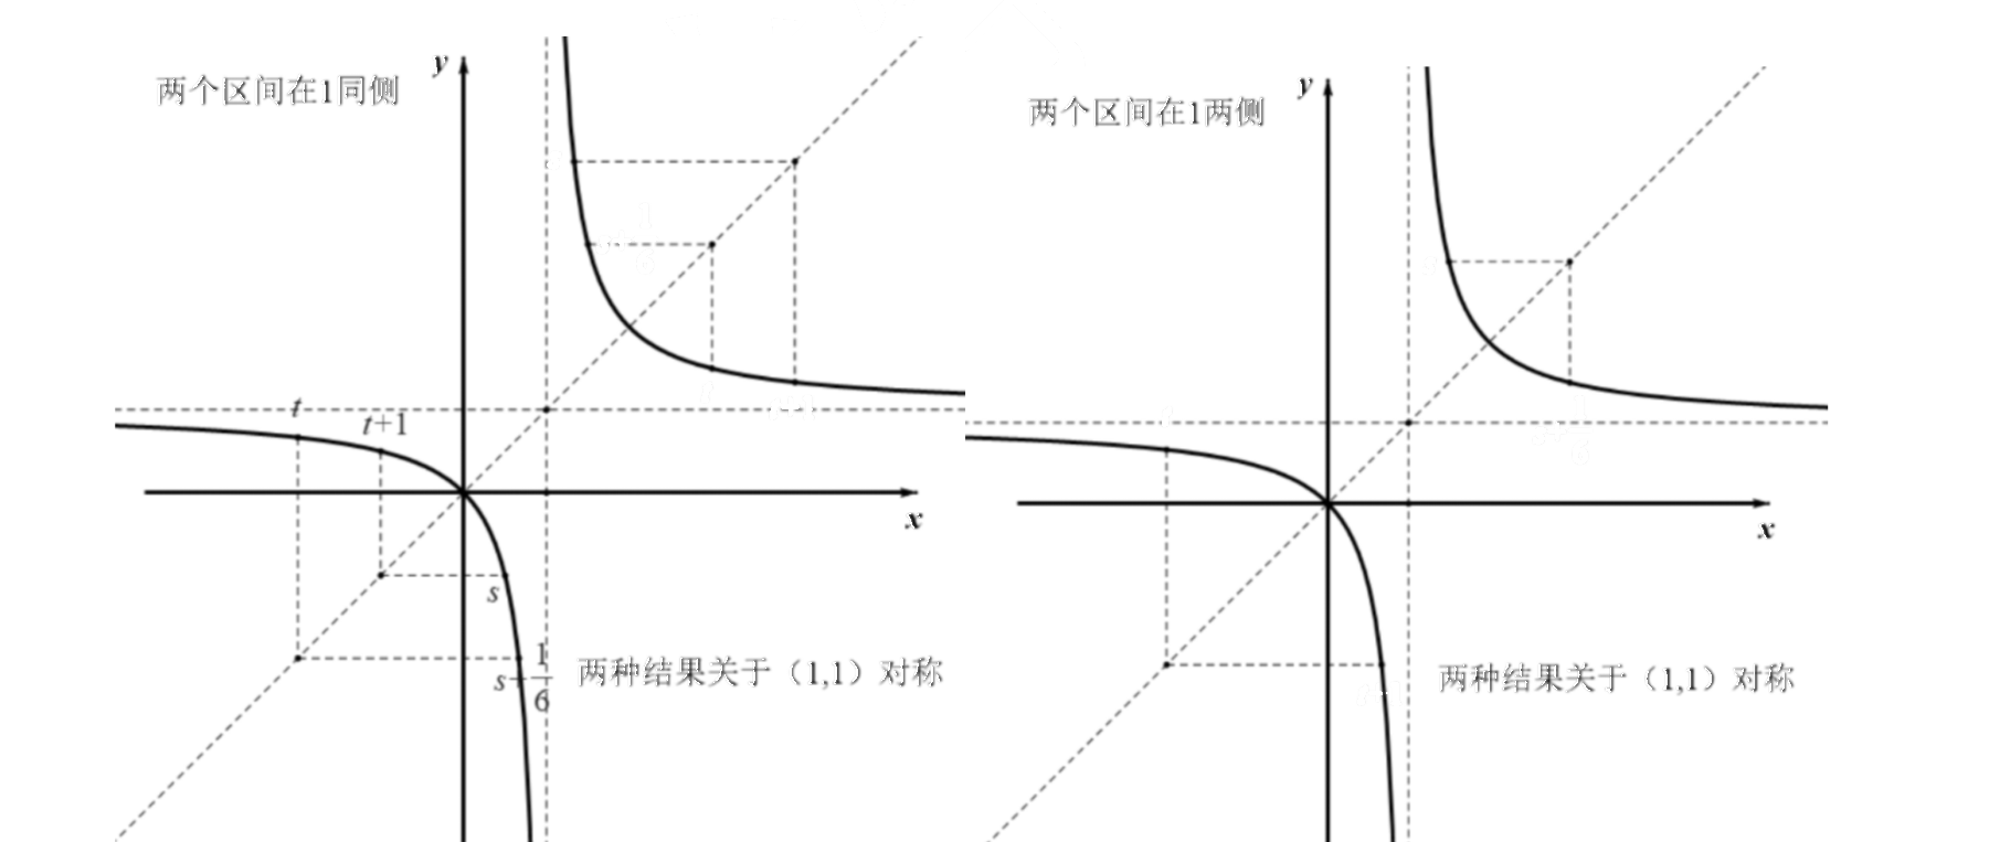
\includegraphics[width=0.92\textwidth]{figures/gao115_q10.png}
\end{center}
\solend
\fi

\end{enumerate}

\bigsec{二、选择题}

\begin{enumerate}
\setcounter{enumi}{10}

\item “对任意有理数 $x$ 都有 $x^2\neq2$”的否定形式是\mbox{（\quad）}% 原卷把答案“$B$”印在题干括号内、无【解析】

\keepwithprev
A. 存在有理数 $x$ 使得 $x^2\neq2$\qquad\qquad B. 存在有理数 $x$ 使得 $x^2=2$

C. 存在无理数 $x$ 使得 $x^2\neq2$\qquad\qquad D. 存在无理数 $x$ 使得 $x^2=2$

\ifanswer
\ans{$B$}
\fi

\item 已知 $a$、$b$ 都是实数，那么“$a^3>b^3$”是“$a^2>b^2$”的\mbox{（\quad）}

\keepwithprev
A. 充分不必要条件\qquad\qquad B. 必要不充分条件

C. 充要条件\qquad\qquad\qquad D. 既不充分也不必要条件

\ifanswer
\solbegin
\step{因为 $a^3>b^3$ 等价于 $a>b$，}
\step{由于 $a$、$b$ 正负不定，所以由 $a>b$ 不能得到 $a^2>b^2$，}
\step{由 $a^2>b^2$ 也不能得到 $a>b$，}
\step{因此“$a^3>b^3$”是“$a^2>b^2$”的既不充分也不必要条件. 故选 $D$.}
\solend
\fi

\item 定义集合运算 $A-B=\{x\mid x\in A$ 且 $x\notin B\}$，将 $A\triangle B=(A-B)\cup(B-A)$ 称为集合 $A$ 与集合 $B$ 的对称差.

命题一：$A\triangle B=B\triangle A$；

命题二：$A\triangle\varnothing=A$；

命题三：$A\cap(B\triangle C)=(A\cap B)\triangle(A\cap C)$；

命题四：$A\cup(B\triangle C)=(A\cup B)\triangle(A\cup C)$；

其中正确命题的个数是\mbox{（\quad）}

\keepwithprev
A. $1$\qquad\qquad B. $2$\qquad\qquad C. $3$\qquad\qquad D. $4$

\ifanswer
\solbegin
\step{对于①，$B\triangle A=(B-A)\cup(A-B)=(A-B)\cup(B-A)=A\triangle B$，①对；}
\step{对于②，$A-B=\{x\mid x\in A$ 且 $x\notin B\}=\{x\mid x\in A$ 且 $x\notin(A\cap B)\}$}
\step{$=A-(A\cap B)$，则 $A\triangle\varnothing=(A-\varnothing)\cup(\varnothing-A)=A\cup\varnothing=A$，②对；}
\step{对于③，$A\cap(B\triangle C)=A\cap(B\cup C-B\cap C)=A\cap(B\cup C)-A\cap(B\cap C)$}
\step{$=(A\cap B)\cup(A\cap C)-(A\cap B)\cap(A\cap C)=(A\cap B)\triangle(A\cap C)$，③对；}
\step{对于④，如图所示：}
\begin{center}
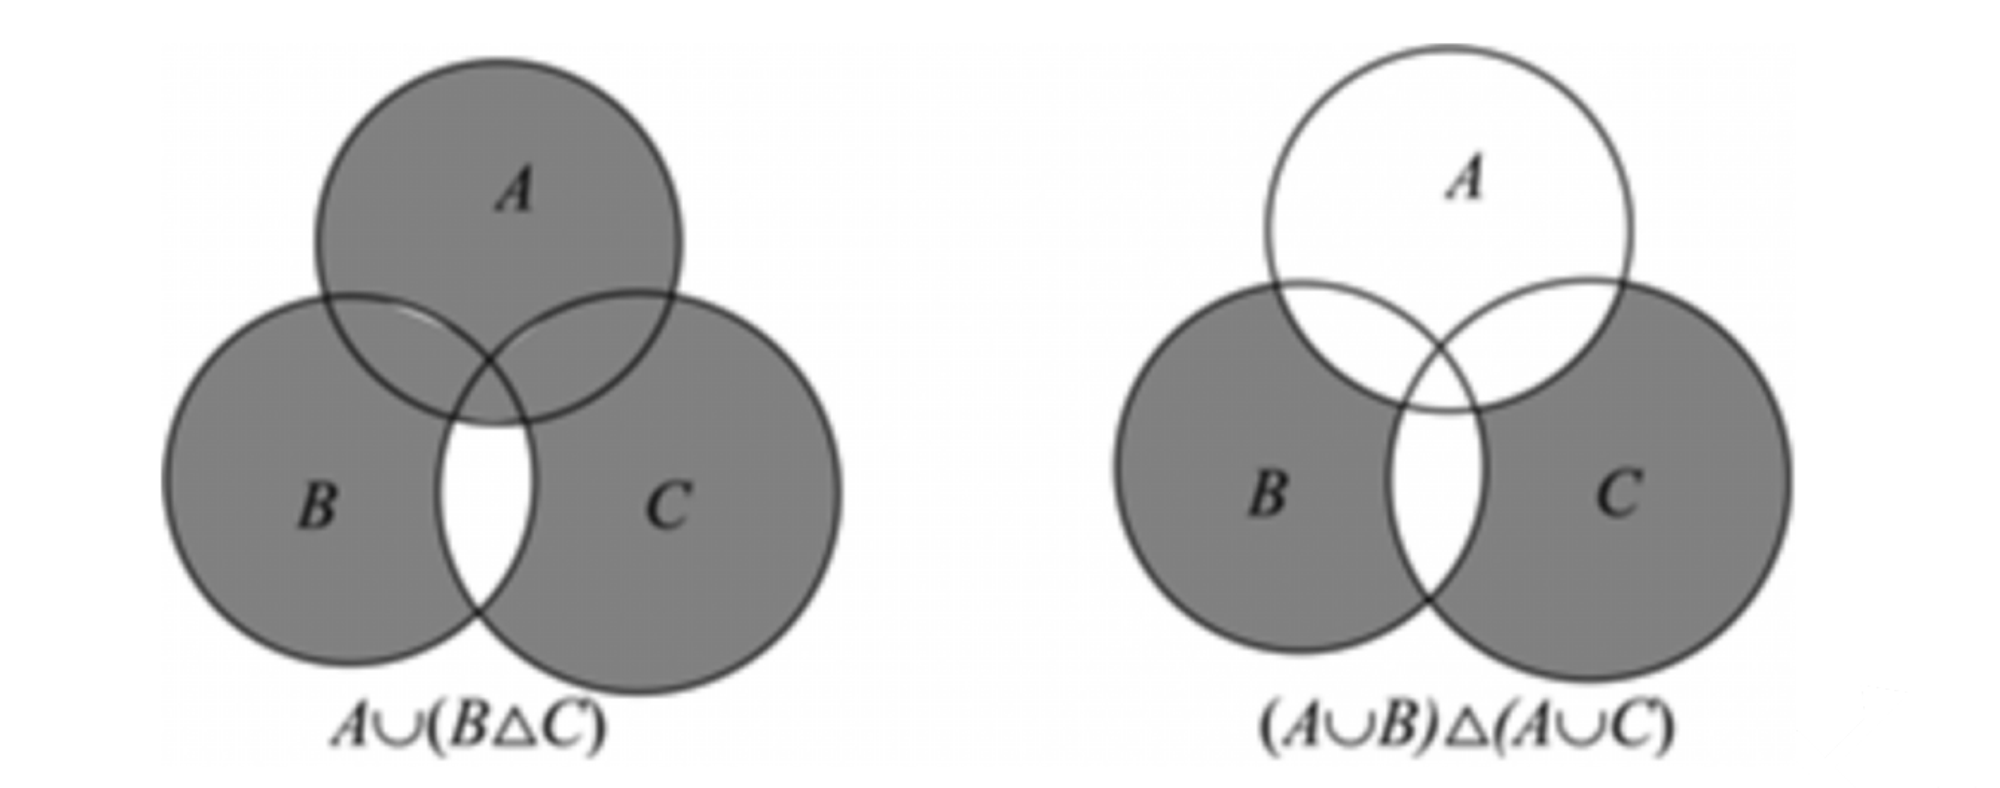
\includegraphics[width=0.85\textwidth]{figures/gao115_q13.png}
\end{center}
\step{所以 $A\cup(B\triangle C)\neq(A\cup B)\triangle(A\cup C)$，④错.}
\step{故选 $C$.}
\solend
\fi

\item 设 $a$、$b$、$c$、$p$ 为实数，若同时满足不等式 $ax^2+bx+c>0$、$bx^2+cx+a>0$ 与 $cx^2+ax+b>0$ 的全体实数 $x$ 所组成的集合等于 $(p,+\infty)$，则关于结论：① $a$、$b$、$c$ 至少有一个为 $0$；② $p=0$. 下列判断中正确的是\mbox{（\quad）}

\keepwithprev
A. ①和②都正确\qquad B. ①和②都错误\qquad C. ①正确，②错误\qquad D. ①错误，②正确

\ifanswer
\solbegin
\step{若同时满足不等式 $ax^2+bx+c>0$、$bx^2+cx+a>0$ 与 $cx^2+ax+b>0$ 的}
\step{全体实数 $x$ 所组成的集合等于 $(p,+\infty)$，必有 $a$,$b$,$c\geqslant0$，}
\step{不妨假设 $a$、$b$、$c$ 没有一个为 $0$，}
\step{则三个不等式均为开口向上的二次函数大于 $0$ 的部分，}
\step{解集的交集应为 $(-\infty,m)\cup(n,+\infty)$ 的形式，矛盾，}
\step{所以 $a$、$b$、$c$ 至少有一个为 $0$，故①正确：}
\step{不妨设 $a=0$，则 $b$,$c\geqslant0$，则不等式组化为 $\begin{cases}bx+c>0\\bx^2+cx>0,\\cx^2+b>0\end{cases}$}
\step{所以 $\begin{cases}x>-\dfrac cb\\x<-\dfrac cb\text{或}x>0\\x\in\R\end{cases}$，取交集得 $(0,+\infty)$，故 $p=0$，故②正确：}
\step{故选 $A$.}
\solend
\fi

\end{enumerate}

\bigsec{三、解答题}

\begin{enumerate}
\setcounter{enumi}{14}

\item 已知 $a>0$，$b>0$，

（1）试比较 $\dfrac{a^2-b^2}{a^2+b^2}$ 与 $\dfrac{a-b}{a+b}$ 的大小；

（2）若 $a+b>4$，求证：$\dfrac a{b+2}$ 和 $\dfrac b{a+2}$ 中至少有一个大于 $\dfrac12$.

\ifanswer
\solbegin
\step{（1）已知 $a>0$，$b>0$，$\dfrac{a^2-b^2}{a^2+b^2}-\dfrac{a-b}{a+b}=\dfrac{2ab(a-b)}{(a^2+b^2)(a+b)}$，}
\step{当 $a>b$ 时，$a-b>0$，所以 $\dfrac{a^2-b^2}{a^2+b^2}-\dfrac{a-b}{a+b}>0$，所以 $\dfrac{a^2-b^2}{a^2+b^2}>\dfrac{a-b}{a+b}$；}
\step{当 $a=b$ 时，$a-b=0$，所以 $\dfrac{a^2-b^2}{a^2+b^2}-\dfrac{a-b}{a+b}=0$，所以 $\dfrac{a^2-b^2}{a^2+b^2}=\dfrac{a-b}{a+b}$；}
\step{当 $a<b$ 时，$a-b<0$，所以 $\dfrac{a^2-b^2}{a^2+b^2}-\dfrac{a-b}{a+b}<0$，所以 $\dfrac{a^2-b^2}{a^2+b^2}<\dfrac{a-b}{a+b}$；}
\step{（2）假设 $\dfrac a{b+2}$ 和 $\dfrac b{a+2}$ 中都不大于 $\dfrac12$，即 $\dfrac b{a+2}\leqslant\dfrac12$，$\dfrac a{b+2}\leqslant\dfrac12$，}
\step{因为 $a>0$，$b>0$，所以 $a+2>0$，$b+2>0$，}
\step{所以 $2b\leqslant a+2$，$2a\leqslant b+2$，}
\step{两式相加得 $2a+2b\leqslant a+2+b+2=a+b+4$，即 $a+b\leqslant4$，}
\step{与已知 $a+b>4$ 矛盾，所以假设错误，}
\step{故 $\dfrac a{b+2}$ 和 $\dfrac b{a+2}$ 中至少有一个大于 $\dfrac12$.}
\solend
\fi

\item 某企业原有 $200$ 名科技人员，年人均工资 $a$ 万元($a>0$). 现加大对某芯片研发力度，该企业把原有 $200$ 名科技人员调整成技术人员和研发人员，其中技术人员 $x$ 名($x\in\N$ 且 $40\leqslant x\leqslant80$). 调整后，研发人员的年人均工资比调整前增加了 $(2x)\%$，技术人员的年人均工资为 $a\left(m-\dfrac x{10}\right)$万元.

（1）若要使调整后研发人员的年总工资不低于调整前 $200$ 名科技人员年总工资的 $1.5$ 倍，求调整后的技术人员最少有多少人？

（2）为了激励研发人员的工作热情和保持技术人员的工作积极性，企业决定在工资方面要同时满足以下两个条件：

①研发人员的年总工资始终不低于技术人员的年总工资；

②技术人员的年人均工资始终不低于调整前 $200$ 名科技人员的年人均工资.

请问是否存在这样的实数 $m$？若存在，求出 $m$ 的范围；若不存在，说明理由.

\ifanswer
\solbegin
\step{（1）由题意得调整后研发人员的年人均工资为 $[1+(2x)\%]a$ 万元，}
\step{那么 $(200-x)[1+(2x)\%]a\geqslant1.5\times200a$ ($a>0$)，}
\step{化简得 $x^2-150x+5000\leqslant0$，解得 $50\leqslant x\leqslant100$，}
\step{由于 $x\in\N$ 且 $40\leqslant x\leqslant80$，因此 $50\leqslant x\leqslant80$，}
\step{因此调整后的技术人员的人数最少为 $50$ 人；}
\step{（2）假设存在实数 $m$，使得技术人员在已知范围内调整后，满足以上两个条件，}
\step{由条件①得 $(200-x)[1+(2x)\%]a\geqslant x\left(m-\dfrac x{10}\right)a$，}
\step{整理得 $m\leqslant\dfrac{200}{x}+\dfrac{2x}{25}+3$；}
\step{因为 $\dfrac{200}{x}+\dfrac{2x}{25}+3\geqslant2\sqrt{\dfrac{200}{x}\cdot\dfrac{2x}{25}}+3=11$，}
\step{当且仅当 $\dfrac{200}{x}=\dfrac{2x}{25}$，即 $x=50$ 时取等号，因此 $m\leqslant11$，}
\step{由条件②得 $a\left(m-\dfrac x{10}\right)\geqslant a$，所以 $m\geqslant\dfrac x{10}+1$；}
\step{又由于 $40\leqslant x\leqslant80$，因此 $m\geqslant9$.}
\step{因此 $m\in[9,11]$.}
\solend
\fi

\item 已知 $a\in\R$，记 $f(x)=ax^2-(a+2)x+2$.

（1）若 $f(x)<3-2x$ 对于一切 $x\in\R$ 恒成立，求实数 $a$ 的取值范围；

（2）求关于 $x$ 不等式 $f(x)\geqslant0$ 的解集；

（3）若存在 $m\in\R$ 使关于 $x$ 的方程 $ax^2-(a+2)\lvert x\rvert+2=\lvert m+2\rvert+\lvert m-1\rvert$ 有四个不同的实根，求实数 $a$ 的取值范围.

\ifanswer
\solbegin
\step{（1）由 $f(x)<3-2x$ 对于一切 $x\in\R$ 恒成立，}
\step{得 $ax^2-ax-1<0$ 对于一切 $x\in\R$ 恒成立，}
\step{当 $a=0$ 时，原式可化为 $-1<0$，恒成立，符合条件；}
\step{当 $a\neq0$ 时，需满足 $\begin{cases}a<0\\\Delta=a^2+4a<0\end{cases}$，解得 $-4<a<0$；}
\step{综上，实数 $a$ 的取值范围是 $(-4,0]$；}
\step{（2）$f(x)\geqslant0$，即 $(ax-2)(x-1)\geqslant0$，}
\step{当 $a=0$ 时，原式化为 $-2x+2\geqslant0$，解集为 $\{x\mid x\leqslant1\}$；}
\step{当 $a>0$ 时，若 $a=2$，原式化为 $2(x-1)^2\geqslant0$，解集为 $\R$；}
\step{若 $0<a<2$，$\dfrac2a>1$，解集为 $\{x\mid x\leqslant1$ 或 $x\geqslant\dfrac2a\}$；}
\step{若 $a>2$，$\dfrac2a<1$，解集为 $\{x\mid x\leqslant\dfrac2a$ 或 $x\geqslant1\}$；}
\step{当 $a<0$ 时，$\dfrac2a<1$，解集为 $\left\{x\,\middle\vert\,\dfrac2a\leqslant x\leqslant1\right\}$；}
\step{综上，当 $a<0$ 时，不等式解集为 $\left\{x\,\middle\vert\,\dfrac2a\leqslant x\leqslant1\right\}$；}
\step{当 $a=0$ 时，不等式解集为 $\{x\mid x\leqslant1\}$；}
\step{当 $0<a<2$ 时，不等式解集为 $\{x\mid x\leqslant1$ 或 $x\geqslant\dfrac2a\}$；}
\step{当 $a=2$ 时，不等式解集为 $\R$；}
\step{当 $a>2$ 时，不等式解集为 $\{x\mid x\leqslant\dfrac2a$ 或 $x\geqslant1\}$；}
\step{（3）由绝对值三角不等式得 $\lvert m+2\rvert+\lvert m-1\rvert\geqslant\lvert(m+2)-(m-1)\rvert=3$，}
\step{即右侧取值范围为 $[3,+\infty)$，}
\step{令 $t=\lvert x\rvert\geqslant0$，原方程转化为 $at^2-(a+2)t+2=k$，$k\in[3,+\infty)$，}
\step{若原方程有四个不同实根，}
\step{需存在 $k\geqslant3$，使得方程 $at^2-(a+2)t+2-k=0$ 有两个不同正实根，}
\step{当 $a\geqslant0$ 时，方程的两根之积为 $\dfrac{2-k}{a}$，}
\step{因为 $k\geqslant3$，所以 $2-k\leqslant-1<0$，两根一正一负，}
\step{最多只有一个正根，对应最多两个 $x$ 根，不符合要求；}
\step{当 $a<0$ 时，两根之积为正，}
\step{要两个根都为正，需要两根之和 $\dfrac{a+2}{a}>0$，解得 $a<-2$，}
\step{再要求存在 $k\geqslant3$ 使得判别式大于 $0$，}
\step{即 $\triangle=(a+2)^2-4a(2-k)>0$ 在 $k\in[3,+\infty)$ 上有解，}
\step{即 $(a-2)^2+4ak>0$ 在 $k\in[3,+\infty)$ 上有解，}
\step{由 $a<0$，得 $(a-2)^2+12a>0$，}
\step{即 $a^2+8a+4>0$，结合 $a<-2$ 解得 $a<-4-2\sqrt3$，}
\step{故实数 $a$ 的取值范围是 $(-\infty,-4-2\sqrt3)$.}
\solend
\fi

\item 设 $A=\{x_1,x_2,\cdots,x_n\}(n\geqslant2,n\in\N)$，且 $x_1,x_2,\cdots,x_n$ 均为正整数，若对于 $A$ 中任意两个元素 $a,b$，当 $a>b$ 时，都有 $\dfrac{b^2}{a-b}\in A$，则称 $A$ 为“$n$ 元好集”.

（1）判断 $\{2,4,6\}$ 是否为“三元好集”，并说明理由；

（2）若集合 $M$ 为“二元好集”，且 $M$ 中所有元素之积小于 $2026$，求所有满足条件的集合 $M$ 的个数；

（3）设 $k\geqslant3,k\in\N$，是否存在“$k$ 元好集”，若存在，求出所有满足条件的“$k$ 元好集”，若不存在，请说明理由.

\ifanswer
\solbegin
\step{（1）取 $a=6,b=2$，则 $\dfrac{b^2}{a-b}=\dfrac44=1\notin\{2,4,6\}$，所以该集合不是三元好集.}
\step{（2）设 $M=\{b,a\}$，其中 $a>b$ 且均为正整数，则 $\dfrac{b^2}{a-b}$ 等于 $a$ 或 $b$.}
\step{若 $\dfrac{b^2}{a-b}=a$，则 $a^2-ab-b^2=0$，从而 $\dfrac ab=\dfrac{1+\sqrt5}{2}$，与 $\dfrac ab$ 为有理数矛盾.}
\step{若 $\dfrac{b^2}{a-b}=b$，则 $a=2b$；}
\step{反之，任意正整数 $b$ 对应的 $\{b,2b\}$ 均为二元好集.}
\step{由元素之积小于 $2026$，得 $2b^2<2026\Leftrightarrow b^2<1013$.}
\step{因为 $31^2=961<1013<1024=32^2$，所以 $b=1,2,\cdots,31$，}
\step{对应 $31$ 个不同的集合.}
\step{（3）假设存在 $k\geqslant3$ 的 $k$ 元好集 $A$，将其元素从小到大排列，}
\step{记最小元素为 $u$，次小元素为 $v$，最大元素为 $w$，则 $0<u<v<w$.}
\step{由 $\dfrac{u^2}{w-u}\in A$，该数不小于 $u$，得 $\dfrac{u^2}{w-u}\geqslant u\Rightarrow w\leqslant2u$.}
\step{又由 $\dfrac{u^2}{v-u}$,$\dfrac{v^2}{w-v}\in A$，这两个数均不超过 $w$，}
\step{得 $\dfrac{u^2}{v-u}\leqslant w$,$\dfrac{v^2}{w-v}\leqslant w$，}
\step{分母均为正，分别去分母后相加，}
\step{得 $u^2+v^2\leqslant w(v-u)+w(w-v)=w(w-u)\leqslant2u^2$，}
\step{于是 $v^2\leqslant u^2$，与 $v>u>0$ 矛盾，所以不存在 $k\geqslant3$ 的 $k$ 元好集.}
\solend
\fi

\end{enumerate}

\end{document}
"
%
% 原始材料：微信公众号“魔都数学加油站”文章，作者破晓，2026-11-06 17:58 发布；
% 连载“27学年高一115”，原文标题“27学年高一115——2026-2027年上海市复旦附中高一上10月阶段练习”；
% 原文链接：https://mp.weixin.qq.com/s/krocP0fMQQ4VM1SQEcLI2Q。
% 正文为 12 张 PNG 页（第 4、6、12 页 2560×3620，其余 4762×6735），
% 题目下印有【解析】或【答案】，为讲评版。
% 题目、解析均据原图转录；卷面红色水印及公众号页脚未录入。
%
% 卷首标题：原卷印作“2026-2027 年复旦附中高一上 10 月阶段练习”（公众号标题中的“上海市”
% 卷面标题行没有，本稿照卷面），年份区间按全稿惯例排 en dash；原卷未印副标题，本稿按题目内容
% 标为“集合与常用逻辑用语、不等式”。
%
% 与原卷的排版差异：
%   ① 原文从第 3 题起，填空题编号为 3—10、选择题为 11—14、解答题为 15—18，共 16 题，
%      本稿保留原题号（与多数卷的 3—21 不同）；
%   ② 原卷每题下直接印【解析】／【答案】，本稿按全稿惯例置于答案版；第 11 题把答案“$B$”
%      印在题干括号内且无【解析】，另提 \ans{}；其余选择题答案在解析末句“故选 …”，括号内留空；
%   ③ 原卷未印副标题，本稿按“知识模块”口径补出；
%   ④ 原卷填空横线按全稿惯例排为 \blankline[4.4em]；选择题括号排 \mbox{（\quad）}、
%      选项段前按惯例加 \keepwithprev；解答题不留作答区（原卷为讲评版，与 109—114 同）；
%   ⑤ 原卷数集排斜体 $R$／$Q$／$N$，按全稿惯例改 \R、\Q、\N。
%
% 判别式与对称差字形：原卷 $\triangle$（等边、扁）与 $\Delta$（等腰、高）两种混用，逐处照录——
%   第 7 题与第 17 题 (3) 的判别式、第 13 题的对称差 $A\triangle B$ 用 \triangle，
%   第 17 题 (1) cases 的判别式用 \Delta。
%
% 子集符号：第 4 题解析的 $(-1,3)\subset(-m,m)$ 印单线（真子集、无下划线），按 18／96
%   成例照录 \subset；第 5 题解析的 $B\subseteq A$ 印有下划线，照录 \subseteq。
%   第 3 题的补集照原卷上划线排 \overline{N}。
%
% 原卷存疑照录：第 9 题解析末行“故可能成立的是①②③”与四种情形的编号一致，照录；
%   第 10 题解析两幅函数图上另有蓝色／红色手写标注（$t$、$t+1$、$s$、$\frac16$ 等），
%   系批改笔迹，随裁图保留、不另作正文录入；第 14 题解析的 cases 三行照原卷排；
%   第 18 题 (2) 解析“所以该集合不是三元好集”前的取例 $a=6,b=2$ 照录。
%
% 行数核对：逐题数 \step/\stepm 条数，合计 133 条（Q3：3；Q4：3；Q5：4；Q6：5；Q7：4；
% Q8：4；Q9：11；Q10：7；Q11：0；Q12：4；Q13：8；Q14：9；Q15：10；Q16：13；
% Q17：32；Q18：16），与原卷印刷行逐题相等（cases 块作一个印刷行计）。第 11 题括号内印
% 答案且无解析，提 \ans{}，不计入 \step 账；第 10、13 题解析内的插图不计入 \step 账。
%
\documentclass[a4paper,11pt]{article}
\usepackage{common}

\begin{document}

\examtitlest[3]{2026--2027 年复旦附中高一上 10 月阶段练习}{集合与常用逻辑用语、不等式}

\bigsec{一、填空题}

\begin{enumerate}
\setcounter{enumi}{2}

\item 已知集合 $M=\{x\mid 4x^2-4x-15>0\}$，$N=\left\{x\,\middle\vert\,\dfrac{x+1}{x-6}>0\right\}$，则 $M\cap\overline{N}=$\blankline[4.4em].

\ifanswer
\solbegin
\step{集合 $M=\{x\mid 4x^2-4x-15>0\}=\{x\mid x>\dfrac52$ 或 $x<-\dfrac32\}$，}
\step{$N=\left\{x\,\middle\vert\,\dfrac{x+1}{x-6}>0\right\}=\{x\mid x>6$ 或 $x<-1\}$，得 $\overline{N}=\{x\mid-1\leqslant x\leqslant6\}$，}
\step{故 $M\cap\overline{N}=\left\{x\,\middle\vert\,\dfrac52<x\leqslant6\right\}$.}
\solend
\fi

\item 已知 $m>0$，不等式 $\lvert x\rvert<m$ 成立的一个充分不必要条件是 $-1<x<3$，则 $m$ 的取值范围是\blankline[4.4em].

\ifanswer
\solbegin
\step{不等式 $-m<x<m$ 成立的一个充分不必要条件是 $-1<x<3$，}
\step{由题意得 $(-1,3)\subset(-m,m)$，则 $m\geqslant3$，此时 $-m\leqslant-3<-1$，}% 原卷印单线 \subset，照录
\step{所以 $m$ 的取值范围是 $\{m\mid m\geqslant3\}$.}
\solend
\fi

\item 已知集合 $A=\{1,2\}$，集合 $B=\{x\mid ax=6\}$，若 $A\cup B=A$，则 $a$ 的所有取值构成的集合为\blankline[4.4em].

\ifanswer
\solbegin
\step{因为 $A\cup B=A$，所以 $B\subseteq A$，}
\step{当 $a=0$ 时，$B=\varnothing$，满足 $B\subseteq A$；}
\step{当 $a\neq0$ 时，$B=\left\{\dfrac6a\right\}$，则 $\dfrac6a=1$ 或 $\dfrac6a=2$，解得 $a=6$ 或 $a=3$，}
\step{综上所述，$a$ 的所有取值构成的集合为 $\{0,3,6\}$.}
\solend
\fi

\item 若关于 $x$ 的不等式 $ax^2+bx+c>0$ 的解集为 $(-3,2)$，则不等式 $ax^2+(a+b)x+c-2a>0$ 的解集为\blankline[4.4em].

\ifanswer
\solbegin
\step{由 $ax^2+bx+c>0$ 的解集为 $(-3,2)$ 得 $a<0$，}
\step{且 $ax^2+bx+c=0$ 时 $x_1=-3$，$x_2=2$，}
\step{得 $-3+2=-\dfrac ba$，即 $b=a$，$-3\times2=\dfrac ca$，即 $c=-6a$，}
\step{代入 $ax^2+(a+b)x+c-2a>0$ 得 $ax^2+2ax-8a>0$ 化简得 $x^2+2x-8<0$，}
\step{解得 $-4<x<2$，故解集为 $(-4,2)$.}
\solend
\fi

\item 已知关于 $x$ 的方程 $x^2-2x+m=0$ 的两个实数根分别为 $x_1$，$x_2$. 若 $x_1^2x_2^2+x_1^2+x_2^2=7$，则实数 $m$ 的值为\blankline[4.4em].

\ifanswer
\solbegin
\step{由韦达定理得 $x_1+x_2=2$，$x_1x_2=m$，}
\step{$x_1^2x_2^2+x_1^2+x_2^2=(x_1x_2)^2+(x_1+x_2)^2-2x_1x_2=m^2+4-2m$，}
\step{由 $m^2+4-2m=7$，得 $m^2-2m-3=0$，解得 $m=3$ 或 $m=-1$，}
\step{方程有两个实数根，故 $\triangle=4-4m\geqslant0$，即 $m\leqslant1$，所以 $m=-1$.}
\solend
\fi

\item 已知 $x>1$，若 $x^2-xy+y=0$，则 $x+y$ 的最小值是\blankline[4.4em].

\ifanswer
\solbegin
\step{由于 $x^2-xy+y=0$，则 $y=\dfrac{x^2}{x-1}>0$，}
\step{则 $x+y=x+\dfrac{x^2}{x-1}=\dfrac{2x^2-x}{x-1}=\dfrac{2(x-1)^2+3(x-1)+1}{x-1}$}
\step{$=2(x-1)+\dfrac1{x-1}+3\geqslant2\sqrt{2(x-1)\cdot\dfrac1{x-1}}+3=2\sqrt2+3$，}
\step{当且仅当 $x=1+\dfrac{\sqrt2}{2}$ 时取等号，故最小值是 $2\sqrt2+3$.}
\solend
\fi

\item 若集合 $A=B_1\cup B_2\cup\cdots\cup B_n$，其中 $B_1$、$B_2$、$\cdots$、$B_n$ 为非空集合，$B_i\cap B_j=\varnothing$，$1\leqslant i<j\leqslant n$，则称集合 $\{B_1,B_2,\cdots,B_n\}$ 为集合 $A$ 的一个 $n$ 划分. 例如：集合 $\{\{1,2\},\{3\}\}$，$\{\{1,3\},\{2\}\}$，$\{\{2,3\},\{1\}\}$ 均为集合 $\{1,2,3\}$ 的一个 $2$ 划分. 设 $\{B_1,B_2\}$ 为有理数集 $\Q$ 的一个 $2$ 划分，且满足对任意 $x\in B_1$，任意 $y\in B_2$，都有 $x<y$. 则对于 $B_1$、$B_2$ 有：

① $B_1$ 中的元素存在最大值，$B_2$ 中的元素不存在最小值；

② $B_1$ 中的元素不存在最大值，$B_2$ 中的元素存在最小值；

③ $B_1$ 中的元素不存在最大值，$B_2$ 中的元素不存在最小值；

④ $B_1$ 中的元素存在最大值，$B_2$ 中的元素存在最小值；

对于以上四种情况，可能成立的序号有\blankline[4.4em].

\ifanswer
\solbegin
\step{对于①，$B_1=\{x\in\Q\mid x\leqslant2\}$，$B_2=\{x\in\Q\mid x>2\}$，①可能成立；}
\step{对于②，$B_1=\{x\in\Q\mid x<2\}$，$B_2=\{x\in\Q\mid x\geqslant2\}$，②可能成立；}
\step{对于③，$B_1=\{x\in\Q\mid x<\pi\}$，$B_2=\{x\in\Q\mid x>\pi\}$，③可能成立；}
\step{对于④，假设④成立，}
\step{不妨设 $B_1$ 中的元素的最大值为 $s$，$B_2$ 中的元素的最小值为 $t$，}
\step{由题意得 $s<t$，所以 $s<\dfrac{s+t}{2}<t$，}
\step{因为 $s$ 为 $B_1$ 中的元素的最大值，所以 $\dfrac{s+t}{2}\notin B_1$，}
\step{因为 $t$ 为 $B_2$ 中的元素的最小值，所以 $\dfrac{s+t}{2}\notin B_2$，}
\step{又 $B_1\cup B_2=\Q$，所以 $\dfrac{s+t}{2}\notin\Q$，与 $\dfrac{s+t}{2}\in\Q$ 矛盾，}
\step{所以假设不成立，即④不可能成立.}
\step{故可能成立的是①②③.}
\solend
\fi

\item 已知集合 $A=\left[s,s+\dfrac16\right]\cup[t,t+1]$，其中 $1\notin A$ 且 $s+\dfrac16<t$，函数 $f(x)=\dfrac x{x-1}$，且对任意 $a\in A$，都有 $f(a)\in A$，则 $t$ 的值是\blankline[4.4em].

\ifanswer
\solbegin
\step{若 $\left[s,s+\dfrac16\right]$,$[t,t+1]$ 在 $f(x)=\dfrac x{x-1}$ 图像的同侧，}
\step{则点 $\left(t,s+\dfrac16\right)$,$(t+1,s)$ 在 $f(x)=\dfrac x{x-1}$ 的图像上，}
\step{所以 $\dfrac t{t-1}=\dfrac{t+1}{t}+\dfrac16$，解得 $t=-2$ 或 $t=3$，检验得 $t=3$；}
\step{若 $\left[s,s+\dfrac16\right]$,$[t,t+1]$ 在 $f(x)=\dfrac x{x-1}$ 图像的两侧，}
\step{则点 $(t,t+1)$ 在 $f(x)=\dfrac x{x-1}$ 的图像上，}
\step{所以 $t+1=\dfrac t{t-1}$，解得 $t=\dfrac{1\pm\sqrt5}{2}$，检验得 $t=\dfrac{1+\sqrt5}{2}$，}
\step{综上，$t=\dfrac{1+\sqrt5}{2}$ 或 $t=3$.}
\begin{center}
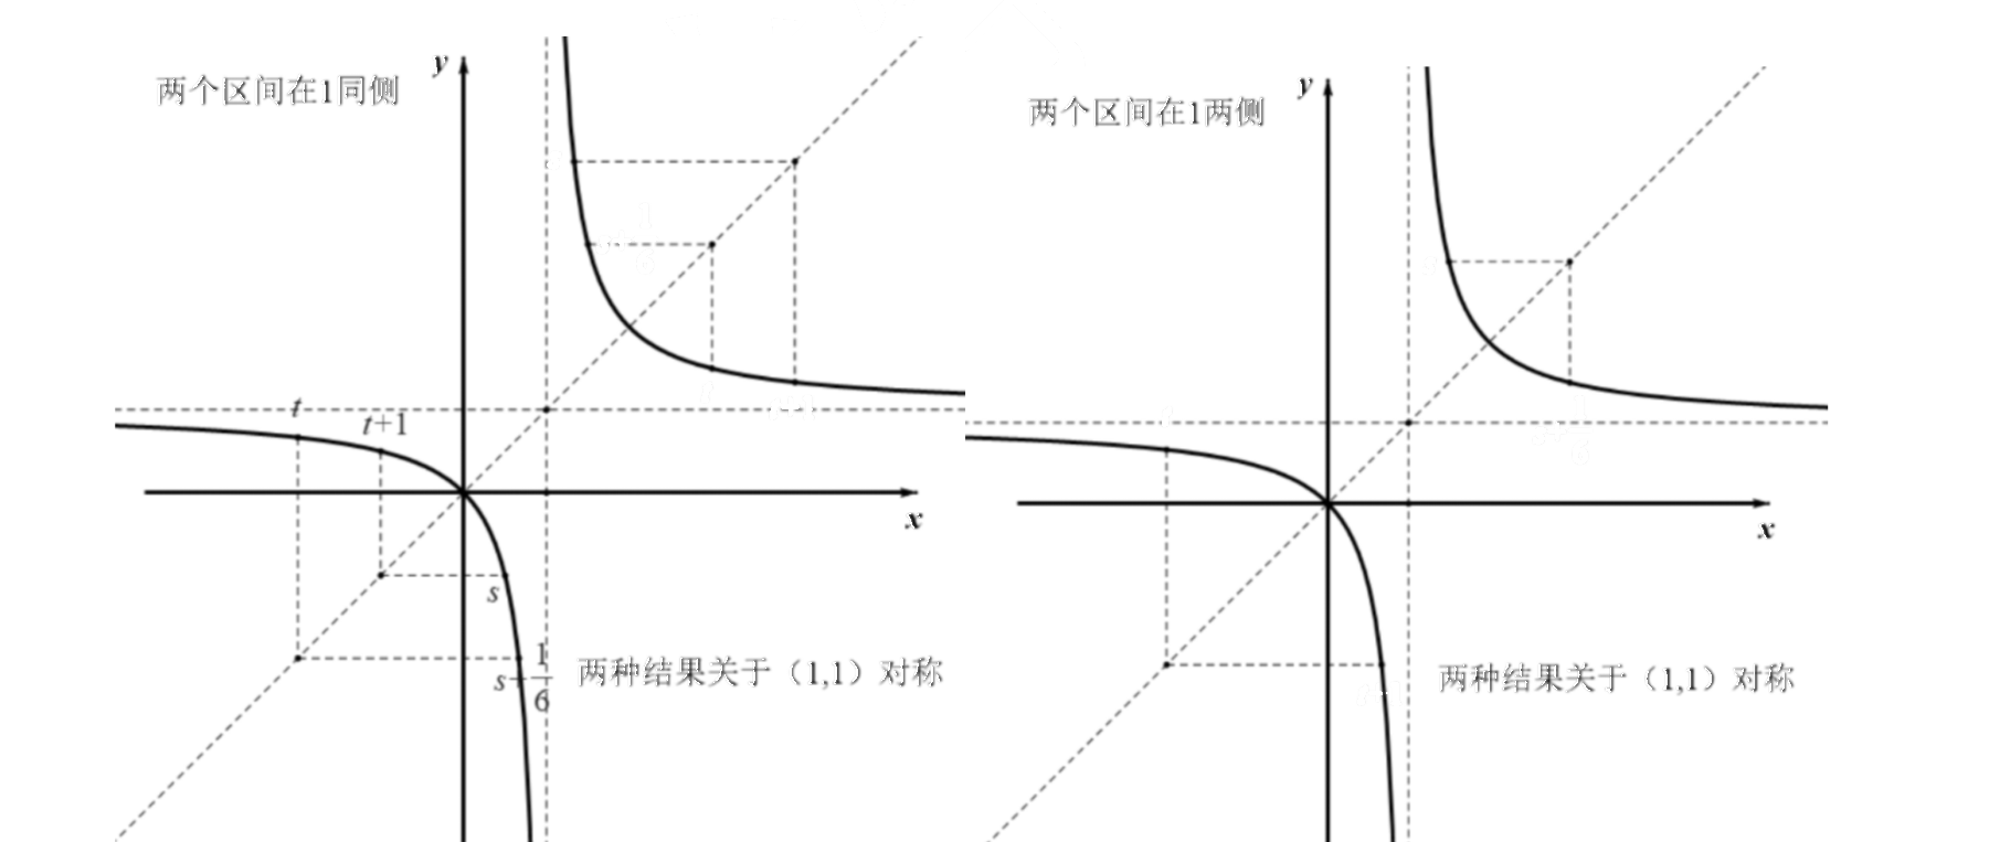
\includegraphics[width=0.92\textwidth]{figures/gao115_q10.png}
\end{center}
\solend
\fi

\end{enumerate}

\bigsec{二、选择题}

\begin{enumerate}
\setcounter{enumi}{10}

\item “对任意有理数 $x$ 都有 $x^2\neq2$”的否定形式是\mbox{（\quad）}% 原卷把答案“$B$”印在题干括号内、无【解析】

\keepwithprev
A. 存在有理数 $x$ 使得 $x^2\neq2$\qquad\qquad B. 存在有理数 $x$ 使得 $x^2=2$

C. 存在无理数 $x$ 使得 $x^2\neq2$\qquad\qquad D. 存在无理数 $x$ 使得 $x^2=2$

\ifanswer
\ans{$B$}
\fi

\item 已知 $a$、$b$ 都是实数，那么“$a^3>b^3$”是“$a^2>b^2$”的\mbox{（\quad）}

\keepwithprev
A. 充分不必要条件\qquad\qquad B. 必要不充分条件

C. 充要条件\qquad\qquad\qquad D. 既不充分也不必要条件

\ifanswer
\solbegin
\step{因为 $a^3>b^3$ 等价于 $a>b$，}
\step{由于 $a$、$b$ 正负不定，所以由 $a>b$ 不能得到 $a^2>b^2$，}
\step{由 $a^2>b^2$ 也不能得到 $a>b$，}
\step{因此“$a^3>b^3$”是“$a^2>b^2$”的既不充分也不必要条件. 故选 $D$.}
\solend
\fi

\item 定义集合运算 $A-B=\{x\mid x\in A$ 且 $x\notin B\}$，将 $A\triangle B=(A-B)\cup(B-A)$ 称为集合 $A$ 与集合 $B$ 的对称差.

命题一：$A\triangle B=B\triangle A$；

命题二：$A\triangle\varnothing=A$；

命题三：$A\cap(B\triangle C)=(A\cap B)\triangle(A\cap C)$；

命题四：$A\cup(B\triangle C)=(A\cup B)\triangle(A\cup C)$；

其中正确命题的个数是\mbox{（\quad）}

\keepwithprev
A. $1$\qquad\qquad B. $2$\qquad\qquad C. $3$\qquad\qquad D. $4$

\ifanswer
\solbegin
\step{对于①，$B\triangle A=(B-A)\cup(A-B)=(A-B)\cup(B-A)=A\triangle B$，①对；}
\step{对于②，$A-B=\{x\mid x\in A$ 且 $x\notin B\}=\{x\mid x\in A$ 且 $x\notin(A\cap B)\}$}
\step{$=A-(A\cap B)$，则 $A\triangle\varnothing=(A-\varnothing)\cup(\varnothing-A)=A\cup\varnothing=A$，②对；}
\step{对于③，$A\cap(B\triangle C)=A\cap(B\cup C-B\cap C)=A\cap(B\cup C)-A\cap(B\cap C)$}
\step{$=(A\cap B)\cup(A\cap C)-(A\cap B)\cap(A\cap C)=(A\cap B)\triangle(A\cap C)$，③对；}
\step{对于④，如图所示：}
\begin{center}
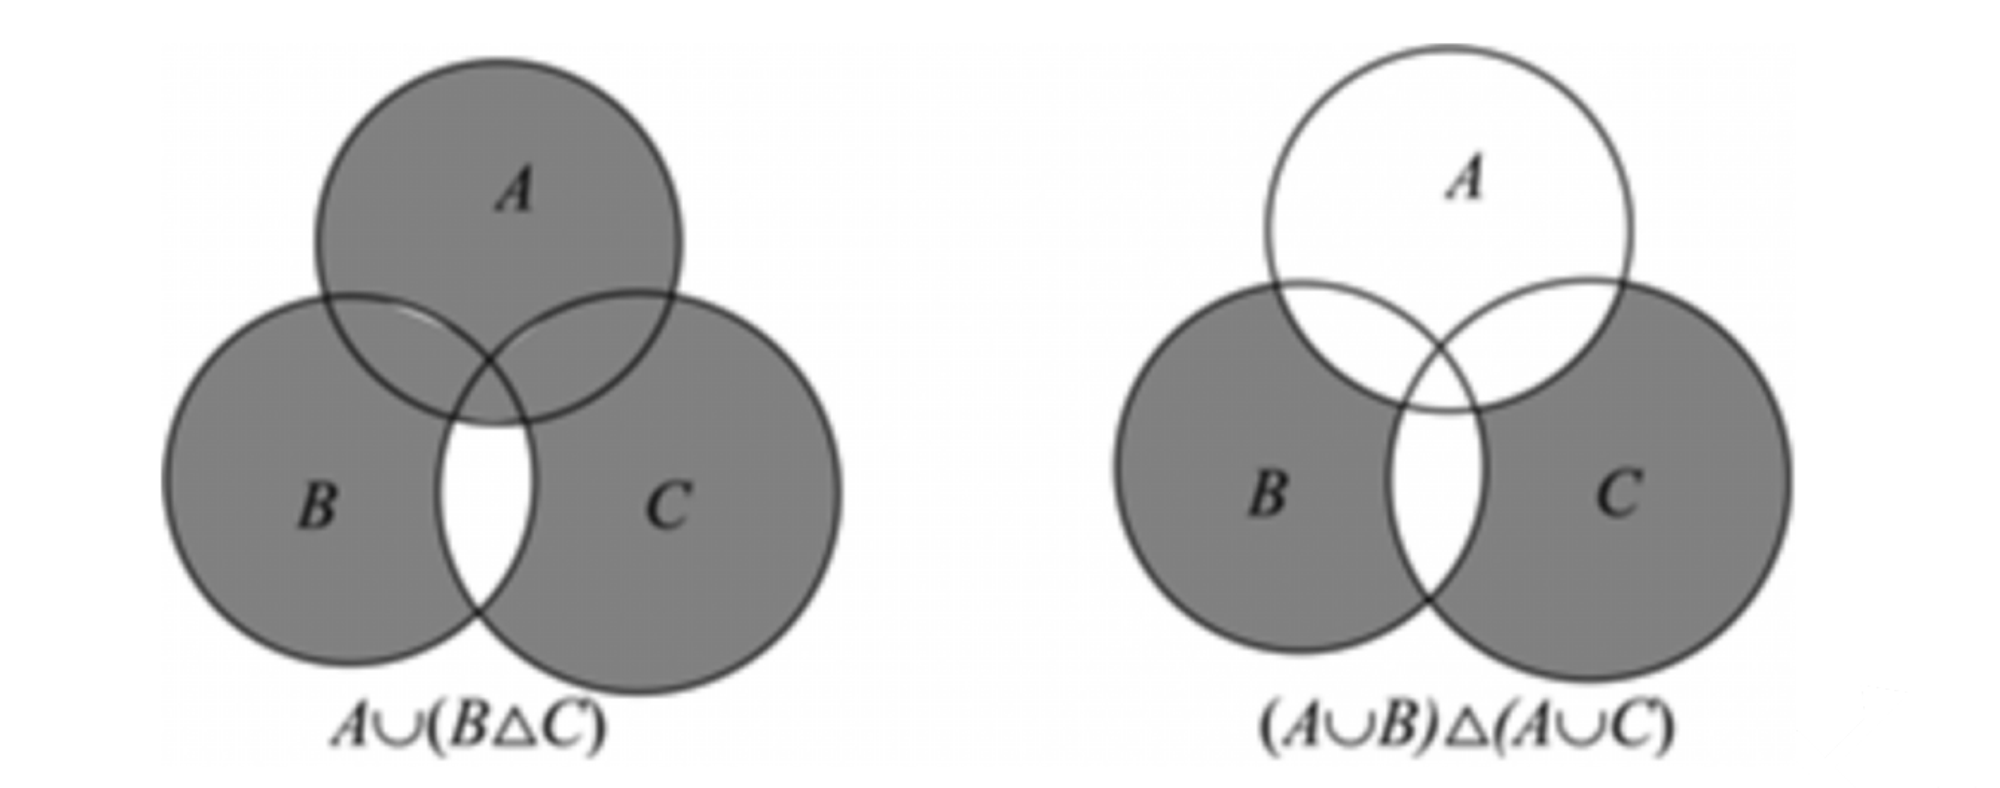
\includegraphics[width=0.85\textwidth]{figures/gao115_q13.png}
\end{center}
\step{所以 $A\cup(B\triangle C)\neq(A\cup B)\triangle(A\cup C)$，④错.}
\step{故选 $C$.}
\solend
\fi

\item 设 $a$、$b$、$c$、$p$ 为实数，若同时满足不等式 $ax^2+bx+c>0$、$bx^2+cx+a>0$ 与 $cx^2+ax+b>0$ 的全体实数 $x$ 所组成的集合等于 $(p,+\infty)$，则关于结论：① $a$、$b$、$c$ 至少有一个为 $0$；② $p=0$. 下列判断中正确的是\mbox{（\quad）}

\keepwithprev
A. ①和②都正确\qquad B. ①和②都错误\qquad C. ①正确，②错误\qquad D. ①错误，②正确

\ifanswer
\solbegin
\step{若同时满足不等式 $ax^2+bx+c>0$、$bx^2+cx+a>0$ 与 $cx^2+ax+b>0$ 的}
\step{全体实数 $x$ 所组成的集合等于 $(p,+\infty)$，必有 $a$,$b$,$c\geqslant0$，}
\step{不妨假设 $a$、$b$、$c$ 没有一个为 $0$，}
\step{则三个不等式均为开口向上的二次函数大于 $0$ 的部分，}
\step{解集的交集应为 $(-\infty,m)\cup(n,+\infty)$ 的形式，矛盾，}
\step{所以 $a$、$b$、$c$ 至少有一个为 $0$，故①正确：}
\step{不妨设 $a=0$，则 $b$,$c\geqslant0$，则不等式组化为 $\begin{cases}bx+c>0\\bx^2+cx>0,\\cx^2+b>0\end{cases}$}
\step{所以 $\begin{cases}x>-\dfrac cb\\x<-\dfrac cb\text{或}x>0\\x\in\R\end{cases}$，取交集得 $(0,+\infty)$，故 $p=0$，故②正确：}
\step{故选 $A$.}
\solend
\fi

\end{enumerate}

\bigsec{三、解答题}

\begin{enumerate}
\setcounter{enumi}{14}

\item 已知 $a>0$，$b>0$，

（1）试比较 $\dfrac{a^2-b^2}{a^2+b^2}$ 与 $\dfrac{a-b}{a+b}$ 的大小；

（2）若 $a+b>4$，求证：$\dfrac a{b+2}$ 和 $\dfrac b{a+2}$ 中至少有一个大于 $\dfrac12$.

\ifanswer
\solbegin
\step{（1）已知 $a>0$，$b>0$，$\dfrac{a^2-b^2}{a^2+b^2}-\dfrac{a-b}{a+b}=\dfrac{2ab(a-b)}{(a^2+b^2)(a+b)}$，}
\step{当 $a>b$ 时，$a-b>0$，所以 $\dfrac{a^2-b^2}{a^2+b^2}-\dfrac{a-b}{a+b}>0$，所以 $\dfrac{a^2-b^2}{a^2+b^2}>\dfrac{a-b}{a+b}$；}
\step{当 $a=b$ 时，$a-b=0$，所以 $\dfrac{a^2-b^2}{a^2+b^2}-\dfrac{a-b}{a+b}=0$，所以 $\dfrac{a^2-b^2}{a^2+b^2}=\dfrac{a-b}{a+b}$；}
\step{当 $a<b$ 时，$a-b<0$，所以 $\dfrac{a^2-b^2}{a^2+b^2}-\dfrac{a-b}{a+b}<0$，所以 $\dfrac{a^2-b^2}{a^2+b^2}<\dfrac{a-b}{a+b}$；}
\step{（2）假设 $\dfrac a{b+2}$ 和 $\dfrac b{a+2}$ 中都不大于 $\dfrac12$，即 $\dfrac b{a+2}\leqslant\dfrac12$，$\dfrac a{b+2}\leqslant\dfrac12$，}
\step{因为 $a>0$，$b>0$，所以 $a+2>0$，$b+2>0$，}
\step{所以 $2b\leqslant a+2$，$2a\leqslant b+2$，}
\step{两式相加得 $2a+2b\leqslant a+2+b+2=a+b+4$，即 $a+b\leqslant4$，}
\step{与已知 $a+b>4$ 矛盾，所以假设错误，}
\step{故 $\dfrac a{b+2}$ 和 $\dfrac b{a+2}$ 中至少有一个大于 $\dfrac12$.}
\solend
\fi

\item 某企业原有 $200$ 名科技人员，年人均工资 $a$ 万元($a>0$). 现加大对某芯片研发力度，该企业把原有 $200$ 名科技人员调整成技术人员和研发人员，其中技术人员 $x$ 名($x\in\N$ 且 $40\leqslant x\leqslant80$). 调整后，研发人员的年人均工资比调整前增加了 $(2x)\%$，技术人员的年人均工资为 $a\left(m-\dfrac x{10}\right)$万元.

（1）若要使调整后研发人员的年总工资不低于调整前 $200$ 名科技人员年总工资的 $1.5$ 倍，求调整后的技术人员最少有多少人？

（2）为了激励研发人员的工作热情和保持技术人员的工作积极性，企业决定在工资方面要同时满足以下两个条件：

①研发人员的年总工资始终不低于技术人员的年总工资；

②技术人员的年人均工资始终不低于调整前 $200$ 名科技人员的年人均工资.

请问是否存在这样的实数 $m$？若存在，求出 $m$ 的范围；若不存在，说明理由.

\ifanswer
\solbegin
\step{（1）由题意得调整后研发人员的年人均工资为 $[1+(2x)\%]a$ 万元，}
\step{那么 $(200-x)[1+(2x)\%]a\geqslant1.5\times200a$ ($a>0$)，}
\step{化简得 $x^2-150x+5000\leqslant0$，解得 $50\leqslant x\leqslant100$，}
\step{由于 $x\in\N$ 且 $40\leqslant x\leqslant80$，因此 $50\leqslant x\leqslant80$，}
\step{因此调整后的技术人员的人数最少为 $50$ 人；}
\step{（2）假设存在实数 $m$，使得技术人员在已知范围内调整后，满足以上两个条件，}
\step{由条件①得 $(200-x)[1+(2x)\%]a\geqslant x\left(m-\dfrac x{10}\right)a$，}
\step{整理得 $m\leqslant\dfrac{200}{x}+\dfrac{2x}{25}+3$；}
\step{因为 $\dfrac{200}{x}+\dfrac{2x}{25}+3\geqslant2\sqrt{\dfrac{200}{x}\cdot\dfrac{2x}{25}}+3=11$，}
\step{当且仅当 $\dfrac{200}{x}=\dfrac{2x}{25}$，即 $x=50$ 时取等号，因此 $m\leqslant11$，}
\step{由条件②得 $a\left(m-\dfrac x{10}\right)\geqslant a$，所以 $m\geqslant\dfrac x{10}+1$；}
\step{又由于 $40\leqslant x\leqslant80$，因此 $m\geqslant9$.}
\step{因此 $m\in[9,11]$.}
\solend
\fi

\item 已知 $a\in\R$，记 $f(x)=ax^2-(a+2)x+2$.

（1）若 $f(x)<3-2x$ 对于一切 $x\in\R$ 恒成立，求实数 $a$ 的取值范围；

（2）求关于 $x$ 不等式 $f(x)\geqslant0$ 的解集；

（3）若存在 $m\in\R$ 使关于 $x$ 的方程 $ax^2-(a+2)\lvert x\rvert+2=\lvert m+2\rvert+\lvert m-1\rvert$ 有四个不同的实根，求实数 $a$ 的取值范围.

\ifanswer
\solbegin
\step{（1）由 $f(x)<3-2x$ 对于一切 $x\in\R$ 恒成立，}
\step{得 $ax^2-ax-1<0$ 对于一切 $x\in\R$ 恒成立，}
\step{当 $a=0$ 时，原式可化为 $-1<0$，恒成立，符合条件；}
\step{当 $a\neq0$ 时，需满足 $\begin{cases}a<0\\\Delta=a^2+4a<0\end{cases}$，解得 $-4<a<0$；}
\step{综上，实数 $a$ 的取值范围是 $(-4,0]$；}
\step{（2）$f(x)\geqslant0$，即 $(ax-2)(x-1)\geqslant0$，}
\step{当 $a=0$ 时，原式化为 $-2x+2\geqslant0$，解集为 $\{x\mid x\leqslant1\}$；}
\step{当 $a>0$ 时，若 $a=2$，原式化为 $2(x-1)^2\geqslant0$，解集为 $\R$；}
\step{若 $0<a<2$，$\dfrac2a>1$，解集为 $\{x\mid x\leqslant1$ 或 $x\geqslant\dfrac2a\}$；}
\step{若 $a>2$，$\dfrac2a<1$，解集为 $\{x\mid x\leqslant\dfrac2a$ 或 $x\geqslant1\}$；}
\step{当 $a<0$ 时，$\dfrac2a<1$，解集为 $\left\{x\,\middle\vert\,\dfrac2a\leqslant x\leqslant1\right\}$；}
\step{综上，当 $a<0$ 时，不等式解集为 $\left\{x\,\middle\vert\,\dfrac2a\leqslant x\leqslant1\right\}$；}
\step{当 $a=0$ 时，不等式解集为 $\{x\mid x\leqslant1\}$；}
\step{当 $0<a<2$ 时，不等式解集为 $\{x\mid x\leqslant1$ 或 $x\geqslant\dfrac2a\}$；}
\step{当 $a=2$ 时，不等式解集为 $\R$；}
\step{当 $a>2$ 时，不等式解集为 $\{x\mid x\leqslant\dfrac2a$ 或 $x\geqslant1\}$；}
\step{（3）由绝对值三角不等式得 $\lvert m+2\rvert+\lvert m-1\rvert\geqslant\lvert(m+2)-(m-1)\rvert=3$，}
\step{即右侧取值范围为 $[3,+\infty)$，}
\step{令 $t=\lvert x\rvert\geqslant0$，原方程转化为 $at^2-(a+2)t+2=k$，$k\in[3,+\infty)$，}
\step{若原方程有四个不同实根，}
\step{需存在 $k\geqslant3$，使得方程 $at^2-(a+2)t+2-k=0$ 有两个不同正实根，}
\step{当 $a\geqslant0$ 时，方程的两根之积为 $\dfrac{2-k}{a}$，}
\step{因为 $k\geqslant3$，所以 $2-k\leqslant-1<0$，两根一正一负，}
\step{最多只有一个正根，对应最多两个 $x$ 根，不符合要求；}
\step{当 $a<0$ 时，两根之积为正，}
\step{要两个根都为正，需要两根之和 $\dfrac{a+2}{a}>0$，解得 $a<-2$，}
\step{再要求存在 $k\geqslant3$ 使得判别式大于 $0$，}
\step{即 $\triangle=(a+2)^2-4a(2-k)>0$ 在 $k\in[3,+\infty)$ 上有解，}
\step{即 $(a-2)^2+4ak>0$ 在 $k\in[3,+\infty)$ 上有解，}
\step{由 $a<0$，得 $(a-2)^2+12a>0$，}
\step{即 $a^2+8a+4>0$，结合 $a<-2$ 解得 $a<-4-2\sqrt3$，}
\step{故实数 $a$ 的取值范围是 $(-\infty,-4-2\sqrt3)$.}
\solend
\fi

\item 设 $A=\{x_1,x_2,\cdots,x_n\}(n\geqslant2,n\in\N)$，且 $x_1,x_2,\cdots,x_n$ 均为正整数，若对于 $A$ 中任意两个元素 $a,b$，当 $a>b$ 时，都有 $\dfrac{b^2}{a-b}\in A$，则称 $A$ 为“$n$ 元好集”.

（1）判断 $\{2,4,6\}$ 是否为“三元好集”，并说明理由；

（2）若集合 $M$ 为“二元好集”，且 $M$ 中所有元素之积小于 $2026$，求所有满足条件的集合 $M$ 的个数；

（3）设 $k\geqslant3,k\in\N$，是否存在“$k$ 元好集”，若存在，求出所有满足条件的“$k$ 元好集”，若不存在，请说明理由.

\ifanswer
\solbegin
\step{（1）取 $a=6,b=2$，则 $\dfrac{b^2}{a-b}=\dfrac44=1\notin\{2,4,6\}$，所以该集合不是三元好集.}
\step{（2）设 $M=\{b,a\}$，其中 $a>b$ 且均为正整数，则 $\dfrac{b^2}{a-b}$ 等于 $a$ 或 $b$.}
\step{若 $\dfrac{b^2}{a-b}=a$，则 $a^2-ab-b^2=0$，从而 $\dfrac ab=\dfrac{1+\sqrt5}{2}$，与 $\dfrac ab$ 为有理数矛盾.}
\step{若 $\dfrac{b^2}{a-b}=b$，则 $a=2b$；}
\step{反之，任意正整数 $b$ 对应的 $\{b,2b\}$ 均为二元好集.}
\step{由元素之积小于 $2026$，得 $2b^2<2026\Leftrightarrow b^2<1013$.}
\step{因为 $31^2=961<1013<1024=32^2$，所以 $b=1,2,\cdots,31$，}
\step{对应 $31$ 个不同的集合.}
\step{（3）假设存在 $k\geqslant3$ 的 $k$ 元好集 $A$，将其元素从小到大排列，}
\step{记最小元素为 $u$，次小元素为 $v$，最大元素为 $w$，则 $0<u<v<w$.}
\step{由 $\dfrac{u^2}{w-u}\in A$，该数不小于 $u$，得 $\dfrac{u^2}{w-u}\geqslant u\Rightarrow w\leqslant2u$.}
\step{又由 $\dfrac{u^2}{v-u}$,$\dfrac{v^2}{w-v}\in A$，这两个数均不超过 $w$，}
\step{得 $\dfrac{u^2}{v-u}\leqslant w$,$\dfrac{v^2}{w-v}\leqslant w$，}
\step{分母均为正，分别去分母后相加，}
\step{得 $u^2+v^2\leqslant w(v-u)+w(w-v)=w(w-u)\leqslant2u^2$，}
\step{于是 $v^2\leqslant u^2$，与 $v>u>0$ 矛盾，所以不存在 $k\geqslant3$ 的 $k$ 元好集.}
\solend
\fi

\end{enumerate}

\end{document}
"
% 紧凑版：xelatex "\def\iscompact{1}% 高一115_复旦附中_10月阶段练习.tex
%   —— 高一上数学“2026-2027 年复旦附中高一上 10 月阶段练习”（试卷版/答案版）
% 试卷版：xelatex 高一115_复旦附中_10月阶段练习.tex
% 答案版：xelatex "\def\isanswer{1}% 高一115_复旦附中_10月阶段练习.tex
%   —— 高一上数学“2026-2027 年复旦附中高一上 10 月阶段练习”（试卷版/答案版）
% 试卷版：xelatex 高一115_复旦附中_10月阶段练习.tex
% 答案版：xelatex "\def\isanswer{1}% 高一115_复旦附中_10月阶段练习.tex
%   —— 高一上数学“2026-2027 年复旦附中高一上 10 月阶段练习”（试卷版/答案版）
% 试卷版：xelatex 高一115_复旦附中_10月阶段练习.tex
% 答案版：xelatex "\def\isanswer{1}\input{高一115_复旦附中_10月阶段练习.tex}"
% 紧凑版：xelatex "\def\iscompact{1}\input{高一115_复旦附中_10月阶段练习.tex}"
%
% 原始材料：微信公众号“魔都数学加油站”文章，作者破晓，2026-11-06 17:58 发布；
% 连载“27学年高一115”，原文标题“27学年高一115——2026-2027年上海市复旦附中高一上10月阶段练习”；
% 原文链接：https://mp.weixin.qq.com/s/krocP0fMQQ4VM1SQEcLI2Q。
% 正文为 12 张 PNG 页（第 4、6、12 页 2560×3620，其余 4762×6735），
% 题目下印有【解析】或【答案】，为讲评版。
% 题目、解析均据原图转录；卷面红色水印及公众号页脚未录入。
%
% 卷首标题：原卷印作“2026-2027 年复旦附中高一上 10 月阶段练习”（公众号标题中的“上海市”
% 卷面标题行没有，本稿照卷面），年份区间按全稿惯例排 en dash；原卷未印副标题，本稿按题目内容
% 标为“集合与常用逻辑用语、不等式”。
%
% 与原卷的排版差异：
%   ① 原文从第 3 题起，填空题编号为 3—10、选择题为 11—14、解答题为 15—18，共 16 题，
%      本稿保留原题号（与多数卷的 3—21 不同）；
%   ② 原卷每题下直接印【解析】／【答案】，本稿按全稿惯例置于答案版；第 11 题把答案“$B$”
%      印在题干括号内且无【解析】，另提 \ans{}；其余选择题答案在解析末句“故选 …”，括号内留空；
%   ③ 原卷未印副标题，本稿按“知识模块”口径补出；
%   ④ 原卷填空横线按全稿惯例排为 \blankline[4.4em]；选择题括号排 \mbox{（\quad）}、
%      选项段前按惯例加 \keepwithprev；解答题不留作答区（原卷为讲评版，与 109—114 同）；
%   ⑤ 原卷数集排斜体 $R$／$Q$／$N$，按全稿惯例改 \R、\Q、\N。
%
% 判别式与对称差字形：原卷 $\triangle$（等边、扁）与 $\Delta$（等腰、高）两种混用，逐处照录——
%   第 7 题与第 17 题 (3) 的判别式、第 13 题的对称差 $A\triangle B$ 用 \triangle，
%   第 17 题 (1) cases 的判别式用 \Delta。
%
% 子集符号：第 4 题解析的 $(-1,3)\subset(-m,m)$ 印单线（真子集、无下划线），按 18／96
%   成例照录 \subset；第 5 题解析的 $B\subseteq A$ 印有下划线，照录 \subseteq。
%   第 3 题的补集照原卷上划线排 \overline{N}。
%
% 原卷存疑照录：第 9 题解析末行“故可能成立的是①②③”与四种情形的编号一致，照录；
%   第 10 题解析两幅函数图上另有蓝色／红色手写标注（$t$、$t+1$、$s$、$\frac16$ 等），
%   系批改笔迹，随裁图保留、不另作正文录入；第 14 题解析的 cases 三行照原卷排；
%   第 18 题 (2) 解析“所以该集合不是三元好集”前的取例 $a=6,b=2$ 照录。
%
% 行数核对：逐题数 \step/\stepm 条数，合计 133 条（Q3：3；Q4：3；Q5：4；Q6：5；Q7：4；
% Q8：4；Q9：11；Q10：7；Q11：0；Q12：4；Q13：8；Q14：9；Q15：10；Q16：13；
% Q17：32；Q18：16），与原卷印刷行逐题相等（cases 块作一个印刷行计）。第 11 题括号内印
% 答案且无解析，提 \ans{}，不计入 \step 账；第 10、13 题解析内的插图不计入 \step 账。
%
\documentclass[a4paper,11pt]{article}
\usepackage{common}

\begin{document}

\examtitlest[3]{2026--2027 年复旦附中高一上 10 月阶段练习}{集合与常用逻辑用语、不等式}

\bigsec{一、填空题}

\begin{enumerate}
\setcounter{enumi}{2}

\item 已知集合 $M=\{x\mid 4x^2-4x-15>0\}$，$N=\left\{x\,\middle\vert\,\dfrac{x+1}{x-6}>0\right\}$，则 $M\cap\overline{N}=$\blankline[4.4em].

\ifanswer
\solbegin
\step{集合 $M=\{x\mid 4x^2-4x-15>0\}=\{x\mid x>\dfrac52$ 或 $x<-\dfrac32\}$，}
\step{$N=\left\{x\,\middle\vert\,\dfrac{x+1}{x-6}>0\right\}=\{x\mid x>6$ 或 $x<-1\}$，得 $\overline{N}=\{x\mid-1\leqslant x\leqslant6\}$，}
\step{故 $M\cap\overline{N}=\left\{x\,\middle\vert\,\dfrac52<x\leqslant6\right\}$.}
\solend
\fi

\item 已知 $m>0$，不等式 $\lvert x\rvert<m$ 成立的一个充分不必要条件是 $-1<x<3$，则 $m$ 的取值范围是\blankline[4.4em].

\ifanswer
\solbegin
\step{不等式 $-m<x<m$ 成立的一个充分不必要条件是 $-1<x<3$，}
\step{由题意得 $(-1,3)\subset(-m,m)$，则 $m\geqslant3$，此时 $-m\leqslant-3<-1$，}% 原卷印单线 \subset，照录
\step{所以 $m$ 的取值范围是 $\{m\mid m\geqslant3\}$.}
\solend
\fi

\item 已知集合 $A=\{1,2\}$，集合 $B=\{x\mid ax=6\}$，若 $A\cup B=A$，则 $a$ 的所有取值构成的集合为\blankline[4.4em].

\ifanswer
\solbegin
\step{因为 $A\cup B=A$，所以 $B\subseteq A$，}
\step{当 $a=0$ 时，$B=\varnothing$，满足 $B\subseteq A$；}
\step{当 $a\neq0$ 时，$B=\left\{\dfrac6a\right\}$，则 $\dfrac6a=1$ 或 $\dfrac6a=2$，解得 $a=6$ 或 $a=3$，}
\step{综上所述，$a$ 的所有取值构成的集合为 $\{0,3,6\}$.}
\solend
\fi

\item 若关于 $x$ 的不等式 $ax^2+bx+c>0$ 的解集为 $(-3,2)$，则不等式 $ax^2+(a+b)x+c-2a>0$ 的解集为\blankline[4.4em].

\ifanswer
\solbegin
\step{由 $ax^2+bx+c>0$ 的解集为 $(-3,2)$ 得 $a<0$，}
\step{且 $ax^2+bx+c=0$ 时 $x_1=-3$，$x_2=2$，}
\step{得 $-3+2=-\dfrac ba$，即 $b=a$，$-3\times2=\dfrac ca$，即 $c=-6a$，}
\step{代入 $ax^2+(a+b)x+c-2a>0$ 得 $ax^2+2ax-8a>0$ 化简得 $x^2+2x-8<0$，}
\step{解得 $-4<x<2$，故解集为 $(-4,2)$.}
\solend
\fi

\item 已知关于 $x$ 的方程 $x^2-2x+m=0$ 的两个实数根分别为 $x_1$，$x_2$. 若 $x_1^2x_2^2+x_1^2+x_2^2=7$，则实数 $m$ 的值为\blankline[4.4em].

\ifanswer
\solbegin
\step{由韦达定理得 $x_1+x_2=2$，$x_1x_2=m$，}
\step{$x_1^2x_2^2+x_1^2+x_2^2=(x_1x_2)^2+(x_1+x_2)^2-2x_1x_2=m^2+4-2m$，}
\step{由 $m^2+4-2m=7$，得 $m^2-2m-3=0$，解得 $m=3$ 或 $m=-1$，}
\step{方程有两个实数根，故 $\triangle=4-4m\geqslant0$，即 $m\leqslant1$，所以 $m=-1$.}
\solend
\fi

\item 已知 $x>1$，若 $x^2-xy+y=0$，则 $x+y$ 的最小值是\blankline[4.4em].

\ifanswer
\solbegin
\step{由于 $x^2-xy+y=0$，则 $y=\dfrac{x^2}{x-1}>0$，}
\step{则 $x+y=x+\dfrac{x^2}{x-1}=\dfrac{2x^2-x}{x-1}=\dfrac{2(x-1)^2+3(x-1)+1}{x-1}$}
\step{$=2(x-1)+\dfrac1{x-1}+3\geqslant2\sqrt{2(x-1)\cdot\dfrac1{x-1}}+3=2\sqrt2+3$，}
\step{当且仅当 $x=1+\dfrac{\sqrt2}{2}$ 时取等号，故最小值是 $2\sqrt2+3$.}
\solend
\fi

\item 若集合 $A=B_1\cup B_2\cup\cdots\cup B_n$，其中 $B_1$、$B_2$、$\cdots$、$B_n$ 为非空集合，$B_i\cap B_j=\varnothing$，$1\leqslant i<j\leqslant n$，则称集合 $\{B_1,B_2,\cdots,B_n\}$ 为集合 $A$ 的一个 $n$ 划分. 例如：集合 $\{\{1,2\},\{3\}\}$，$\{\{1,3\},\{2\}\}$，$\{\{2,3\},\{1\}\}$ 均为集合 $\{1,2,3\}$ 的一个 $2$ 划分. 设 $\{B_1,B_2\}$ 为有理数集 $\Q$ 的一个 $2$ 划分，且满足对任意 $x\in B_1$，任意 $y\in B_2$，都有 $x<y$. 则对于 $B_1$、$B_2$ 有：

① $B_1$ 中的元素存在最大值，$B_2$ 中的元素不存在最小值；

② $B_1$ 中的元素不存在最大值，$B_2$ 中的元素存在最小值；

③ $B_1$ 中的元素不存在最大值，$B_2$ 中的元素不存在最小值；

④ $B_1$ 中的元素存在最大值，$B_2$ 中的元素存在最小值；

对于以上四种情况，可能成立的序号有\blankline[4.4em].

\ifanswer
\solbegin
\step{对于①，$B_1=\{x\in\Q\mid x\leqslant2\}$，$B_2=\{x\in\Q\mid x>2\}$，①可能成立；}
\step{对于②，$B_1=\{x\in\Q\mid x<2\}$，$B_2=\{x\in\Q\mid x\geqslant2\}$，②可能成立；}
\step{对于③，$B_1=\{x\in\Q\mid x<\pi\}$，$B_2=\{x\in\Q\mid x>\pi\}$，③可能成立；}
\step{对于④，假设④成立，}
\step{不妨设 $B_1$ 中的元素的最大值为 $s$，$B_2$ 中的元素的最小值为 $t$，}
\step{由题意得 $s<t$，所以 $s<\dfrac{s+t}{2}<t$，}
\step{因为 $s$ 为 $B_1$ 中的元素的最大值，所以 $\dfrac{s+t}{2}\notin B_1$，}
\step{因为 $t$ 为 $B_2$ 中的元素的最小值，所以 $\dfrac{s+t}{2}\notin B_2$，}
\step{又 $B_1\cup B_2=\Q$，所以 $\dfrac{s+t}{2}\notin\Q$，与 $\dfrac{s+t}{2}\in\Q$ 矛盾，}
\step{所以假设不成立，即④不可能成立.}
\step{故可能成立的是①②③.}
\solend
\fi

\item 已知集合 $A=\left[s,s+\dfrac16\right]\cup[t,t+1]$，其中 $1\notin A$ 且 $s+\dfrac16<t$，函数 $f(x)=\dfrac x{x-1}$，且对任意 $a\in A$，都有 $f(a)\in A$，则 $t$ 的值是\blankline[4.4em].

\ifanswer
\solbegin
\step{若 $\left[s,s+\dfrac16\right]$,$[t,t+1]$ 在 $f(x)=\dfrac x{x-1}$ 图像的同侧，}
\step{则点 $\left(t,s+\dfrac16\right)$,$(t+1,s)$ 在 $f(x)=\dfrac x{x-1}$ 的图像上，}
\step{所以 $\dfrac t{t-1}=\dfrac{t+1}{t}+\dfrac16$，解得 $t=-2$ 或 $t=3$，检验得 $t=3$；}
\step{若 $\left[s,s+\dfrac16\right]$,$[t,t+1]$ 在 $f(x)=\dfrac x{x-1}$ 图像的两侧，}
\step{则点 $(t,t+1)$ 在 $f(x)=\dfrac x{x-1}$ 的图像上，}
\step{所以 $t+1=\dfrac t{t-1}$，解得 $t=\dfrac{1\pm\sqrt5}{2}$，检验得 $t=\dfrac{1+\sqrt5}{2}$，}
\step{综上，$t=\dfrac{1+\sqrt5}{2}$ 或 $t=3$.}
\begin{center}
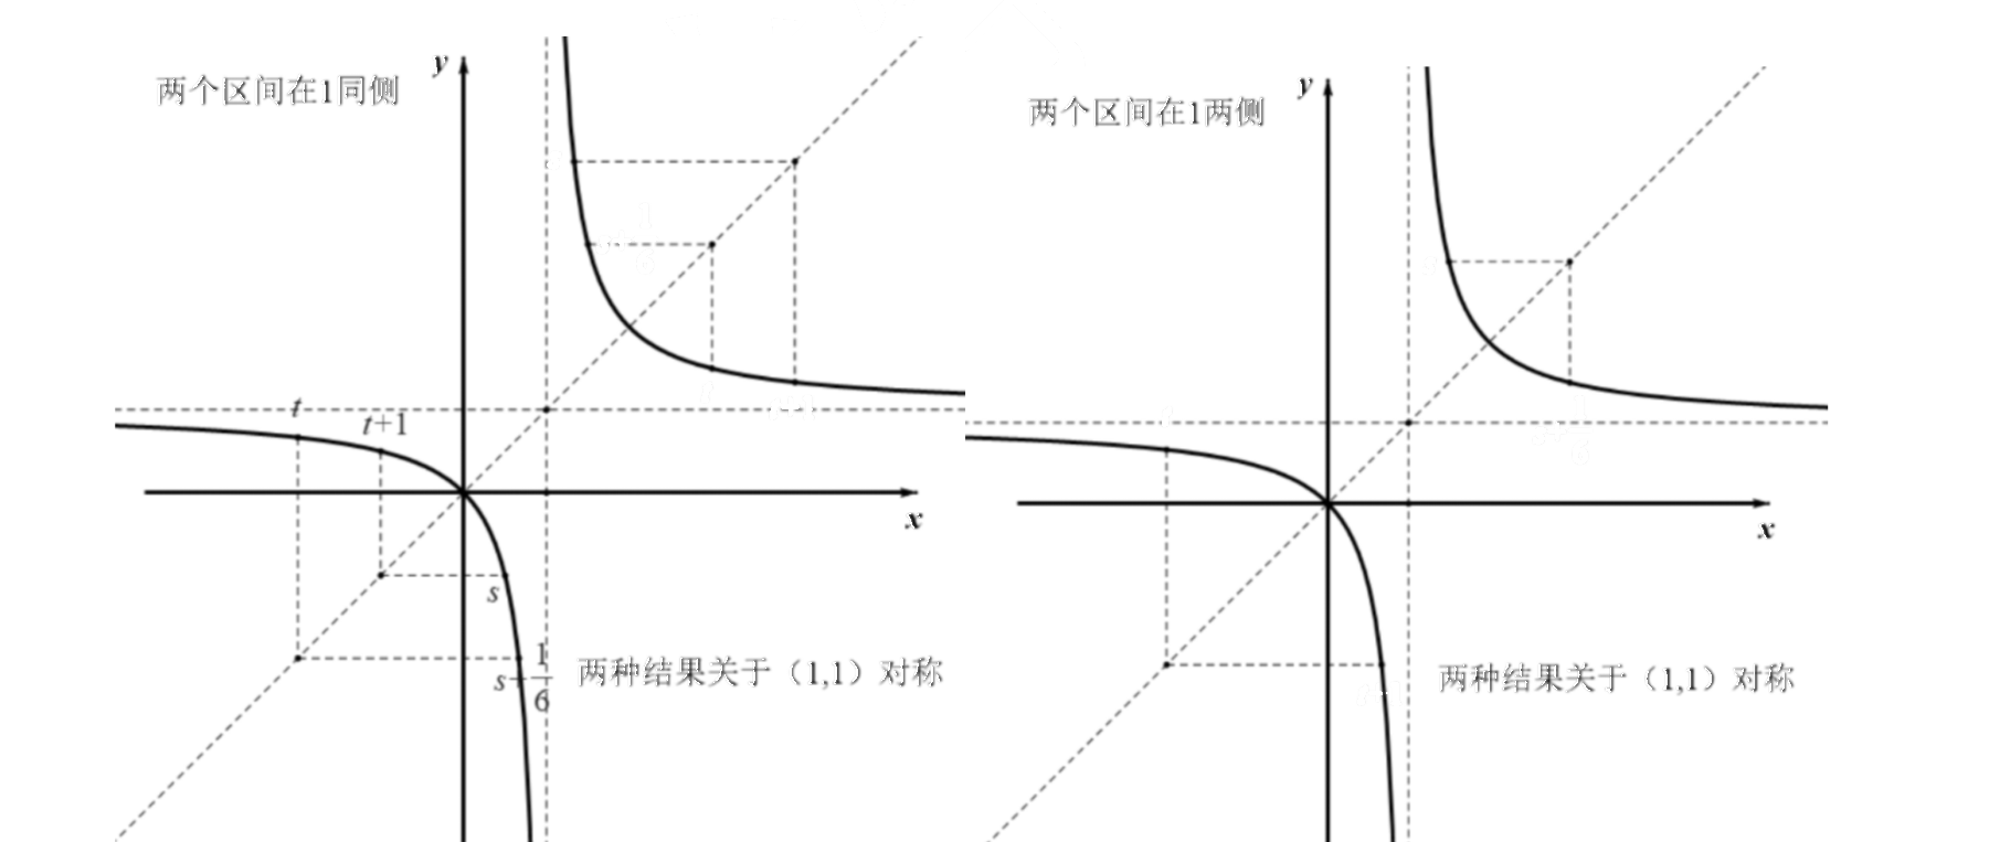
\includegraphics[width=0.92\textwidth]{figures/gao115_q10.png}
\end{center}
\solend
\fi

\end{enumerate}

\bigsec{二、选择题}

\begin{enumerate}
\setcounter{enumi}{10}

\item “对任意有理数 $x$ 都有 $x^2\neq2$”的否定形式是\mbox{（\quad）}% 原卷把答案“$B$”印在题干括号内、无【解析】

\keepwithprev
A. 存在有理数 $x$ 使得 $x^2\neq2$\qquad\qquad B. 存在有理数 $x$ 使得 $x^2=2$

C. 存在无理数 $x$ 使得 $x^2\neq2$\qquad\qquad D. 存在无理数 $x$ 使得 $x^2=2$

\ifanswer
\ans{$B$}
\fi

\item 已知 $a$、$b$ 都是实数，那么“$a^3>b^3$”是“$a^2>b^2$”的\mbox{（\quad）}

\keepwithprev
A. 充分不必要条件\qquad\qquad B. 必要不充分条件

C. 充要条件\qquad\qquad\qquad D. 既不充分也不必要条件

\ifanswer
\solbegin
\step{因为 $a^3>b^3$ 等价于 $a>b$，}
\step{由于 $a$、$b$ 正负不定，所以由 $a>b$ 不能得到 $a^2>b^2$，}
\step{由 $a^2>b^2$ 也不能得到 $a>b$，}
\step{因此“$a^3>b^3$”是“$a^2>b^2$”的既不充分也不必要条件. 故选 $D$.}
\solend
\fi

\item 定义集合运算 $A-B=\{x\mid x\in A$ 且 $x\notin B\}$，将 $A\triangle B=(A-B)\cup(B-A)$ 称为集合 $A$ 与集合 $B$ 的对称差.

命题一：$A\triangle B=B\triangle A$；

命题二：$A\triangle\varnothing=A$；

命题三：$A\cap(B\triangle C)=(A\cap B)\triangle(A\cap C)$；

命题四：$A\cup(B\triangle C)=(A\cup B)\triangle(A\cup C)$；

其中正确命题的个数是\mbox{（\quad）}

\keepwithprev
A. $1$\qquad\qquad B. $2$\qquad\qquad C. $3$\qquad\qquad D. $4$

\ifanswer
\solbegin
\step{对于①，$B\triangle A=(B-A)\cup(A-B)=(A-B)\cup(B-A)=A\triangle B$，①对；}
\step{对于②，$A-B=\{x\mid x\in A$ 且 $x\notin B\}=\{x\mid x\in A$ 且 $x\notin(A\cap B)\}$}
\step{$=A-(A\cap B)$，则 $A\triangle\varnothing=(A-\varnothing)\cup(\varnothing-A)=A\cup\varnothing=A$，②对；}
\step{对于③，$A\cap(B\triangle C)=A\cap(B\cup C-B\cap C)=A\cap(B\cup C)-A\cap(B\cap C)$}
\step{$=(A\cap B)\cup(A\cap C)-(A\cap B)\cap(A\cap C)=(A\cap B)\triangle(A\cap C)$，③对；}
\step{对于④，如图所示：}
\begin{center}
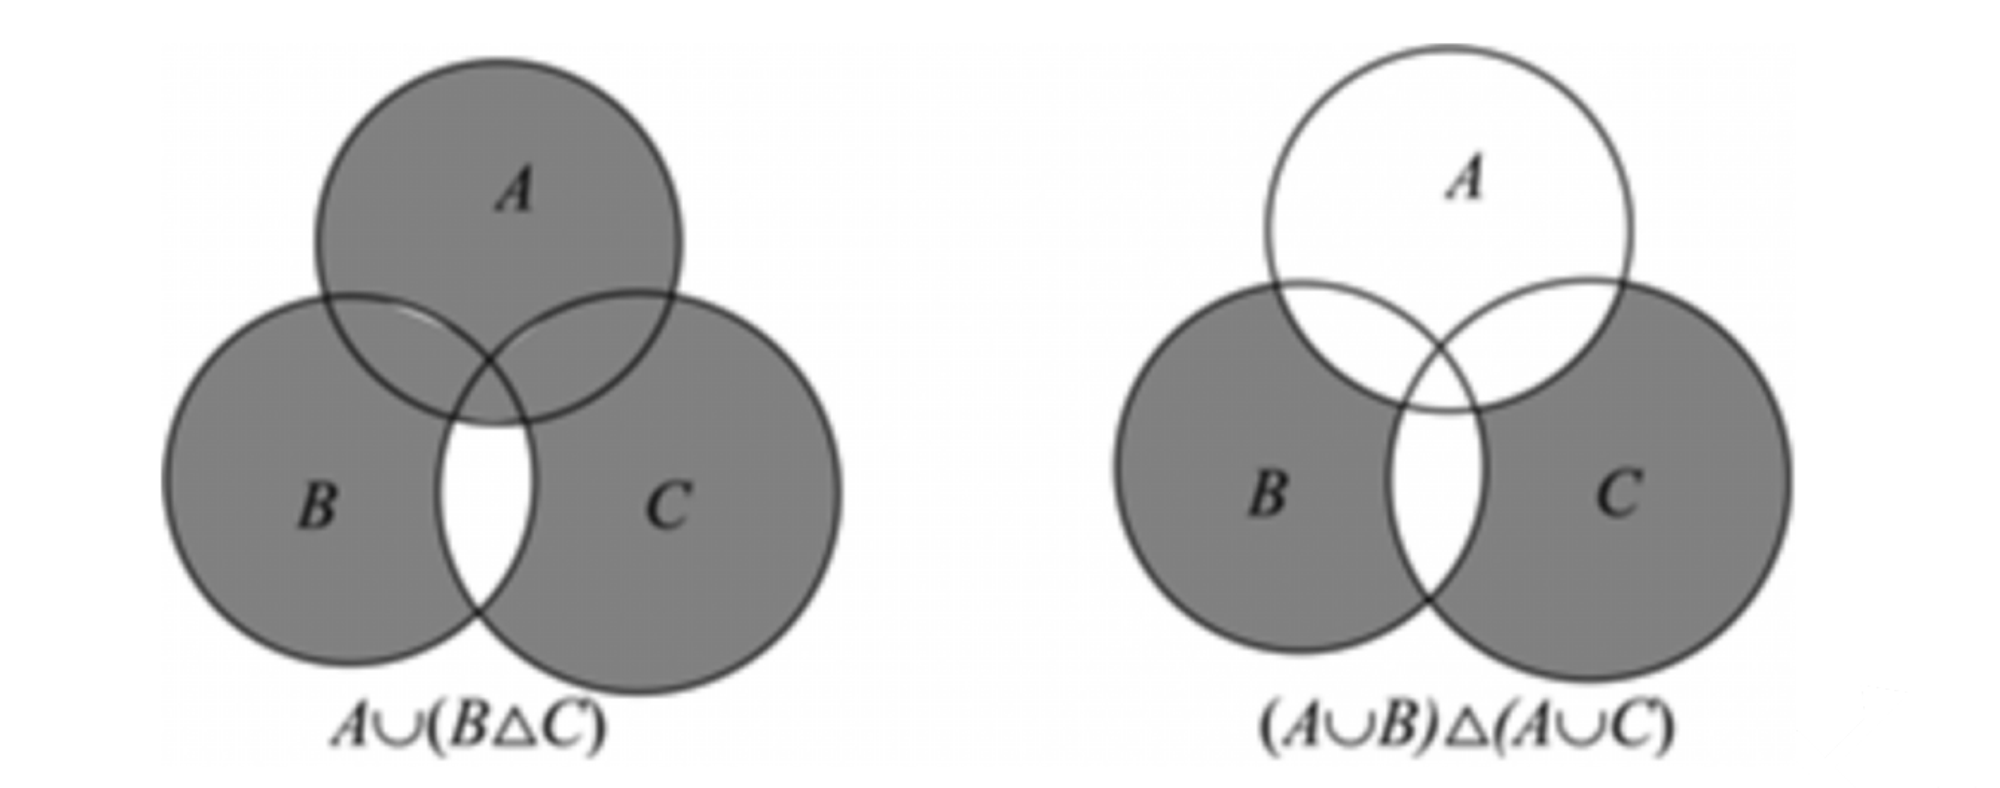
\includegraphics[width=0.85\textwidth]{figures/gao115_q13.png}
\end{center}
\step{所以 $A\cup(B\triangle C)\neq(A\cup B)\triangle(A\cup C)$，④错.}
\step{故选 $C$.}
\solend
\fi

\item 设 $a$、$b$、$c$、$p$ 为实数，若同时满足不等式 $ax^2+bx+c>0$、$bx^2+cx+a>0$ 与 $cx^2+ax+b>0$ 的全体实数 $x$ 所组成的集合等于 $(p,+\infty)$，则关于结论：① $a$、$b$、$c$ 至少有一个为 $0$；② $p=0$. 下列判断中正确的是\mbox{（\quad）}

\keepwithprev
A. ①和②都正确\qquad B. ①和②都错误\qquad C. ①正确，②错误\qquad D. ①错误，②正确

\ifanswer
\solbegin
\step{若同时满足不等式 $ax^2+bx+c>0$、$bx^2+cx+a>0$ 与 $cx^2+ax+b>0$ 的}
\step{全体实数 $x$ 所组成的集合等于 $(p,+\infty)$，必有 $a$,$b$,$c\geqslant0$，}
\step{不妨假设 $a$、$b$、$c$ 没有一个为 $0$，}
\step{则三个不等式均为开口向上的二次函数大于 $0$ 的部分，}
\step{解集的交集应为 $(-\infty,m)\cup(n,+\infty)$ 的形式，矛盾，}
\step{所以 $a$、$b$、$c$ 至少有一个为 $0$，故①正确：}
\step{不妨设 $a=0$，则 $b$,$c\geqslant0$，则不等式组化为 $\begin{cases}bx+c>0\\bx^2+cx>0,\\cx^2+b>0\end{cases}$}
\step{所以 $\begin{cases}x>-\dfrac cb\\x<-\dfrac cb\text{或}x>0\\x\in\R\end{cases}$，取交集得 $(0,+\infty)$，故 $p=0$，故②正确：}
\step{故选 $A$.}
\solend
\fi

\end{enumerate}

\bigsec{三、解答题}

\begin{enumerate}
\setcounter{enumi}{14}

\item 已知 $a>0$，$b>0$，

（1）试比较 $\dfrac{a^2-b^2}{a^2+b^2}$ 与 $\dfrac{a-b}{a+b}$ 的大小；

（2）若 $a+b>4$，求证：$\dfrac a{b+2}$ 和 $\dfrac b{a+2}$ 中至少有一个大于 $\dfrac12$.

\ifanswer
\solbegin
\step{（1）已知 $a>0$，$b>0$，$\dfrac{a^2-b^2}{a^2+b^2}-\dfrac{a-b}{a+b}=\dfrac{2ab(a-b)}{(a^2+b^2)(a+b)}$，}
\step{当 $a>b$ 时，$a-b>0$，所以 $\dfrac{a^2-b^2}{a^2+b^2}-\dfrac{a-b}{a+b}>0$，所以 $\dfrac{a^2-b^2}{a^2+b^2}>\dfrac{a-b}{a+b}$；}
\step{当 $a=b$ 时，$a-b=0$，所以 $\dfrac{a^2-b^2}{a^2+b^2}-\dfrac{a-b}{a+b}=0$，所以 $\dfrac{a^2-b^2}{a^2+b^2}=\dfrac{a-b}{a+b}$；}
\step{当 $a<b$ 时，$a-b<0$，所以 $\dfrac{a^2-b^2}{a^2+b^2}-\dfrac{a-b}{a+b}<0$，所以 $\dfrac{a^2-b^2}{a^2+b^2}<\dfrac{a-b}{a+b}$；}
\step{（2）假设 $\dfrac a{b+2}$ 和 $\dfrac b{a+2}$ 中都不大于 $\dfrac12$，即 $\dfrac b{a+2}\leqslant\dfrac12$，$\dfrac a{b+2}\leqslant\dfrac12$，}
\step{因为 $a>0$，$b>0$，所以 $a+2>0$，$b+2>0$，}
\step{所以 $2b\leqslant a+2$，$2a\leqslant b+2$，}
\step{两式相加得 $2a+2b\leqslant a+2+b+2=a+b+4$，即 $a+b\leqslant4$，}
\step{与已知 $a+b>4$ 矛盾，所以假设错误，}
\step{故 $\dfrac a{b+2}$ 和 $\dfrac b{a+2}$ 中至少有一个大于 $\dfrac12$.}
\solend
\fi

\item 某企业原有 $200$ 名科技人员，年人均工资 $a$ 万元($a>0$). 现加大对某芯片研发力度，该企业把原有 $200$ 名科技人员调整成技术人员和研发人员，其中技术人员 $x$ 名($x\in\N$ 且 $40\leqslant x\leqslant80$). 调整后，研发人员的年人均工资比调整前增加了 $(2x)\%$，技术人员的年人均工资为 $a\left(m-\dfrac x{10}\right)$万元.

（1）若要使调整后研发人员的年总工资不低于调整前 $200$ 名科技人员年总工资的 $1.5$ 倍，求调整后的技术人员最少有多少人？

（2）为了激励研发人员的工作热情和保持技术人员的工作积极性，企业决定在工资方面要同时满足以下两个条件：

①研发人员的年总工资始终不低于技术人员的年总工资；

②技术人员的年人均工资始终不低于调整前 $200$ 名科技人员的年人均工资.

请问是否存在这样的实数 $m$？若存在，求出 $m$ 的范围；若不存在，说明理由.

\ifanswer
\solbegin
\step{（1）由题意得调整后研发人员的年人均工资为 $[1+(2x)\%]a$ 万元，}
\step{那么 $(200-x)[1+(2x)\%]a\geqslant1.5\times200a$ ($a>0$)，}
\step{化简得 $x^2-150x+5000\leqslant0$，解得 $50\leqslant x\leqslant100$，}
\step{由于 $x\in\N$ 且 $40\leqslant x\leqslant80$，因此 $50\leqslant x\leqslant80$，}
\step{因此调整后的技术人员的人数最少为 $50$ 人；}
\step{（2）假设存在实数 $m$，使得技术人员在已知范围内调整后，满足以上两个条件，}
\step{由条件①得 $(200-x)[1+(2x)\%]a\geqslant x\left(m-\dfrac x{10}\right)a$，}
\step{整理得 $m\leqslant\dfrac{200}{x}+\dfrac{2x}{25}+3$；}
\step{因为 $\dfrac{200}{x}+\dfrac{2x}{25}+3\geqslant2\sqrt{\dfrac{200}{x}\cdot\dfrac{2x}{25}}+3=11$，}
\step{当且仅当 $\dfrac{200}{x}=\dfrac{2x}{25}$，即 $x=50$ 时取等号，因此 $m\leqslant11$，}
\step{由条件②得 $a\left(m-\dfrac x{10}\right)\geqslant a$，所以 $m\geqslant\dfrac x{10}+1$；}
\step{又由于 $40\leqslant x\leqslant80$，因此 $m\geqslant9$.}
\step{因此 $m\in[9,11]$.}
\solend
\fi

\item 已知 $a\in\R$，记 $f(x)=ax^2-(a+2)x+2$.

（1）若 $f(x)<3-2x$ 对于一切 $x\in\R$ 恒成立，求实数 $a$ 的取值范围；

（2）求关于 $x$ 不等式 $f(x)\geqslant0$ 的解集；

（3）若存在 $m\in\R$ 使关于 $x$ 的方程 $ax^2-(a+2)\lvert x\rvert+2=\lvert m+2\rvert+\lvert m-1\rvert$ 有四个不同的实根，求实数 $a$ 的取值范围.

\ifanswer
\solbegin
\step{（1）由 $f(x)<3-2x$ 对于一切 $x\in\R$ 恒成立，}
\step{得 $ax^2-ax-1<0$ 对于一切 $x\in\R$ 恒成立，}
\step{当 $a=0$ 时，原式可化为 $-1<0$，恒成立，符合条件；}
\step{当 $a\neq0$ 时，需满足 $\begin{cases}a<0\\\Delta=a^2+4a<0\end{cases}$，解得 $-4<a<0$；}
\step{综上，实数 $a$ 的取值范围是 $(-4,0]$；}
\step{（2）$f(x)\geqslant0$，即 $(ax-2)(x-1)\geqslant0$，}
\step{当 $a=0$ 时，原式化为 $-2x+2\geqslant0$，解集为 $\{x\mid x\leqslant1\}$；}
\step{当 $a>0$ 时，若 $a=2$，原式化为 $2(x-1)^2\geqslant0$，解集为 $\R$；}
\step{若 $0<a<2$，$\dfrac2a>1$，解集为 $\{x\mid x\leqslant1$ 或 $x\geqslant\dfrac2a\}$；}
\step{若 $a>2$，$\dfrac2a<1$，解集为 $\{x\mid x\leqslant\dfrac2a$ 或 $x\geqslant1\}$；}
\step{当 $a<0$ 时，$\dfrac2a<1$，解集为 $\left\{x\,\middle\vert\,\dfrac2a\leqslant x\leqslant1\right\}$；}
\step{综上，当 $a<0$ 时，不等式解集为 $\left\{x\,\middle\vert\,\dfrac2a\leqslant x\leqslant1\right\}$；}
\step{当 $a=0$ 时，不等式解集为 $\{x\mid x\leqslant1\}$；}
\step{当 $0<a<2$ 时，不等式解集为 $\{x\mid x\leqslant1$ 或 $x\geqslant\dfrac2a\}$；}
\step{当 $a=2$ 时，不等式解集为 $\R$；}
\step{当 $a>2$ 时，不等式解集为 $\{x\mid x\leqslant\dfrac2a$ 或 $x\geqslant1\}$；}
\step{（3）由绝对值三角不等式得 $\lvert m+2\rvert+\lvert m-1\rvert\geqslant\lvert(m+2)-(m-1)\rvert=3$，}
\step{即右侧取值范围为 $[3,+\infty)$，}
\step{令 $t=\lvert x\rvert\geqslant0$，原方程转化为 $at^2-(a+2)t+2=k$，$k\in[3,+\infty)$，}
\step{若原方程有四个不同实根，}
\step{需存在 $k\geqslant3$，使得方程 $at^2-(a+2)t+2-k=0$ 有两个不同正实根，}
\step{当 $a\geqslant0$ 时，方程的两根之积为 $\dfrac{2-k}{a}$，}
\step{因为 $k\geqslant3$，所以 $2-k\leqslant-1<0$，两根一正一负，}
\step{最多只有一个正根，对应最多两个 $x$ 根，不符合要求；}
\step{当 $a<0$ 时，两根之积为正，}
\step{要两个根都为正，需要两根之和 $\dfrac{a+2}{a}>0$，解得 $a<-2$，}
\step{再要求存在 $k\geqslant3$ 使得判别式大于 $0$，}
\step{即 $\triangle=(a+2)^2-4a(2-k)>0$ 在 $k\in[3,+\infty)$ 上有解，}
\step{即 $(a-2)^2+4ak>0$ 在 $k\in[3,+\infty)$ 上有解，}
\step{由 $a<0$，得 $(a-2)^2+12a>0$，}
\step{即 $a^2+8a+4>0$，结合 $a<-2$ 解得 $a<-4-2\sqrt3$，}
\step{故实数 $a$ 的取值范围是 $(-\infty,-4-2\sqrt3)$.}
\solend
\fi

\item 设 $A=\{x_1,x_2,\cdots,x_n\}(n\geqslant2,n\in\N)$，且 $x_1,x_2,\cdots,x_n$ 均为正整数，若对于 $A$ 中任意两个元素 $a,b$，当 $a>b$ 时，都有 $\dfrac{b^2}{a-b}\in A$，则称 $A$ 为“$n$ 元好集”.

（1）判断 $\{2,4,6\}$ 是否为“三元好集”，并说明理由；

（2）若集合 $M$ 为“二元好集”，且 $M$ 中所有元素之积小于 $2026$，求所有满足条件的集合 $M$ 的个数；

（3）设 $k\geqslant3,k\in\N$，是否存在“$k$ 元好集”，若存在，求出所有满足条件的“$k$ 元好集”，若不存在，请说明理由.

\ifanswer
\solbegin
\step{（1）取 $a=6,b=2$，则 $\dfrac{b^2}{a-b}=\dfrac44=1\notin\{2,4,6\}$，所以该集合不是三元好集.}
\step{（2）设 $M=\{b,a\}$，其中 $a>b$ 且均为正整数，则 $\dfrac{b^2}{a-b}$ 等于 $a$ 或 $b$.}
\step{若 $\dfrac{b^2}{a-b}=a$，则 $a^2-ab-b^2=0$，从而 $\dfrac ab=\dfrac{1+\sqrt5}{2}$，与 $\dfrac ab$ 为有理数矛盾.}
\step{若 $\dfrac{b^2}{a-b}=b$，则 $a=2b$；}
\step{反之，任意正整数 $b$ 对应的 $\{b,2b\}$ 均为二元好集.}
\step{由元素之积小于 $2026$，得 $2b^2<2026\Leftrightarrow b^2<1013$.}
\step{因为 $31^2=961<1013<1024=32^2$，所以 $b=1,2,\cdots,31$，}
\step{对应 $31$ 个不同的集合.}
\step{（3）假设存在 $k\geqslant3$ 的 $k$ 元好集 $A$，将其元素从小到大排列，}
\step{记最小元素为 $u$，次小元素为 $v$，最大元素为 $w$，则 $0<u<v<w$.}
\step{由 $\dfrac{u^2}{w-u}\in A$，该数不小于 $u$，得 $\dfrac{u^2}{w-u}\geqslant u\Rightarrow w\leqslant2u$.}
\step{又由 $\dfrac{u^2}{v-u}$,$\dfrac{v^2}{w-v}\in A$，这两个数均不超过 $w$，}
\step{得 $\dfrac{u^2}{v-u}\leqslant w$,$\dfrac{v^2}{w-v}\leqslant w$，}
\step{分母均为正，分别去分母后相加，}
\step{得 $u^2+v^2\leqslant w(v-u)+w(w-v)=w(w-u)\leqslant2u^2$，}
\step{于是 $v^2\leqslant u^2$，与 $v>u>0$ 矛盾，所以不存在 $k\geqslant3$ 的 $k$ 元好集.}
\solend
\fi

\end{enumerate}

\end{document}
"
% 紧凑版：xelatex "\def\iscompact{1}% 高一115_复旦附中_10月阶段练习.tex
%   —— 高一上数学“2026-2027 年复旦附中高一上 10 月阶段练习”（试卷版/答案版）
% 试卷版：xelatex 高一115_复旦附中_10月阶段练习.tex
% 答案版：xelatex "\def\isanswer{1}\input{高一115_复旦附中_10月阶段练习.tex}"
% 紧凑版：xelatex "\def\iscompact{1}\input{高一115_复旦附中_10月阶段练习.tex}"
%
% 原始材料：微信公众号“魔都数学加油站”文章，作者破晓，2026-11-06 17:58 发布；
% 连载“27学年高一115”，原文标题“27学年高一115——2026-2027年上海市复旦附中高一上10月阶段练习”；
% 原文链接：https://mp.weixin.qq.com/s/krocP0fMQQ4VM1SQEcLI2Q。
% 正文为 12 张 PNG 页（第 4、6、12 页 2560×3620，其余 4762×6735），
% 题目下印有【解析】或【答案】，为讲评版。
% 题目、解析均据原图转录；卷面红色水印及公众号页脚未录入。
%
% 卷首标题：原卷印作“2026-2027 年复旦附中高一上 10 月阶段练习”（公众号标题中的“上海市”
% 卷面标题行没有，本稿照卷面），年份区间按全稿惯例排 en dash；原卷未印副标题，本稿按题目内容
% 标为“集合与常用逻辑用语、不等式”。
%
% 与原卷的排版差异：
%   ① 原文从第 3 题起，填空题编号为 3—10、选择题为 11—14、解答题为 15—18，共 16 题，
%      本稿保留原题号（与多数卷的 3—21 不同）；
%   ② 原卷每题下直接印【解析】／【答案】，本稿按全稿惯例置于答案版；第 11 题把答案“$B$”
%      印在题干括号内且无【解析】，另提 \ans{}；其余选择题答案在解析末句“故选 …”，括号内留空；
%   ③ 原卷未印副标题，本稿按“知识模块”口径补出；
%   ④ 原卷填空横线按全稿惯例排为 \blankline[4.4em]；选择题括号排 \mbox{（\quad）}、
%      选项段前按惯例加 \keepwithprev；解答题不留作答区（原卷为讲评版，与 109—114 同）；
%   ⑤ 原卷数集排斜体 $R$／$Q$／$N$，按全稿惯例改 \R、\Q、\N。
%
% 判别式与对称差字形：原卷 $\triangle$（等边、扁）与 $\Delta$（等腰、高）两种混用，逐处照录——
%   第 7 题与第 17 题 (3) 的判别式、第 13 题的对称差 $A\triangle B$ 用 \triangle，
%   第 17 题 (1) cases 的判别式用 \Delta。
%
% 子集符号：第 4 题解析的 $(-1,3)\subset(-m,m)$ 印单线（真子集、无下划线），按 18／96
%   成例照录 \subset；第 5 题解析的 $B\subseteq A$ 印有下划线，照录 \subseteq。
%   第 3 题的补集照原卷上划线排 \overline{N}。
%
% 原卷存疑照录：第 9 题解析末行“故可能成立的是①②③”与四种情形的编号一致，照录；
%   第 10 题解析两幅函数图上另有蓝色／红色手写标注（$t$、$t+1$、$s$、$\frac16$ 等），
%   系批改笔迹，随裁图保留、不另作正文录入；第 14 题解析的 cases 三行照原卷排；
%   第 18 题 (2) 解析“所以该集合不是三元好集”前的取例 $a=6,b=2$ 照录。
%
% 行数核对：逐题数 \step/\stepm 条数，合计 133 条（Q3：3；Q4：3；Q5：4；Q6：5；Q7：4；
% Q8：4；Q9：11；Q10：7；Q11：0；Q12：4；Q13：8；Q14：9；Q15：10；Q16：13；
% Q17：32；Q18：16），与原卷印刷行逐题相等（cases 块作一个印刷行计）。第 11 题括号内印
% 答案且无解析，提 \ans{}，不计入 \step 账；第 10、13 题解析内的插图不计入 \step 账。
%
\documentclass[a4paper,11pt]{article}
\usepackage{common}

\begin{document}

\examtitlest[3]{2026--2027 年复旦附中高一上 10 月阶段练习}{集合与常用逻辑用语、不等式}

\bigsec{一、填空题}

\begin{enumerate}
\setcounter{enumi}{2}

\item 已知集合 $M=\{x\mid 4x^2-4x-15>0\}$，$N=\left\{x\,\middle\vert\,\dfrac{x+1}{x-6}>0\right\}$，则 $M\cap\overline{N}=$\blankline[4.4em].

\ifanswer
\solbegin
\step{集合 $M=\{x\mid 4x^2-4x-15>0\}=\{x\mid x>\dfrac52$ 或 $x<-\dfrac32\}$，}
\step{$N=\left\{x\,\middle\vert\,\dfrac{x+1}{x-6}>0\right\}=\{x\mid x>6$ 或 $x<-1\}$，得 $\overline{N}=\{x\mid-1\leqslant x\leqslant6\}$，}
\step{故 $M\cap\overline{N}=\left\{x\,\middle\vert\,\dfrac52<x\leqslant6\right\}$.}
\solend
\fi

\item 已知 $m>0$，不等式 $\lvert x\rvert<m$ 成立的一个充分不必要条件是 $-1<x<3$，则 $m$ 的取值范围是\blankline[4.4em].

\ifanswer
\solbegin
\step{不等式 $-m<x<m$ 成立的一个充分不必要条件是 $-1<x<3$，}
\step{由题意得 $(-1,3)\subset(-m,m)$，则 $m\geqslant3$，此时 $-m\leqslant-3<-1$，}% 原卷印单线 \subset，照录
\step{所以 $m$ 的取值范围是 $\{m\mid m\geqslant3\}$.}
\solend
\fi

\item 已知集合 $A=\{1,2\}$，集合 $B=\{x\mid ax=6\}$，若 $A\cup B=A$，则 $a$ 的所有取值构成的集合为\blankline[4.4em].

\ifanswer
\solbegin
\step{因为 $A\cup B=A$，所以 $B\subseteq A$，}
\step{当 $a=0$ 时，$B=\varnothing$，满足 $B\subseteq A$；}
\step{当 $a\neq0$ 时，$B=\left\{\dfrac6a\right\}$，则 $\dfrac6a=1$ 或 $\dfrac6a=2$，解得 $a=6$ 或 $a=3$，}
\step{综上所述，$a$ 的所有取值构成的集合为 $\{0,3,6\}$.}
\solend
\fi

\item 若关于 $x$ 的不等式 $ax^2+bx+c>0$ 的解集为 $(-3,2)$，则不等式 $ax^2+(a+b)x+c-2a>0$ 的解集为\blankline[4.4em].

\ifanswer
\solbegin
\step{由 $ax^2+bx+c>0$ 的解集为 $(-3,2)$ 得 $a<0$，}
\step{且 $ax^2+bx+c=0$ 时 $x_1=-3$，$x_2=2$，}
\step{得 $-3+2=-\dfrac ba$，即 $b=a$，$-3\times2=\dfrac ca$，即 $c=-6a$，}
\step{代入 $ax^2+(a+b)x+c-2a>0$ 得 $ax^2+2ax-8a>0$ 化简得 $x^2+2x-8<0$，}
\step{解得 $-4<x<2$，故解集为 $(-4,2)$.}
\solend
\fi

\item 已知关于 $x$ 的方程 $x^2-2x+m=0$ 的两个实数根分别为 $x_1$，$x_2$. 若 $x_1^2x_2^2+x_1^2+x_2^2=7$，则实数 $m$ 的值为\blankline[4.4em].

\ifanswer
\solbegin
\step{由韦达定理得 $x_1+x_2=2$，$x_1x_2=m$，}
\step{$x_1^2x_2^2+x_1^2+x_2^2=(x_1x_2)^2+(x_1+x_2)^2-2x_1x_2=m^2+4-2m$，}
\step{由 $m^2+4-2m=7$，得 $m^2-2m-3=0$，解得 $m=3$ 或 $m=-1$，}
\step{方程有两个实数根，故 $\triangle=4-4m\geqslant0$，即 $m\leqslant1$，所以 $m=-1$.}
\solend
\fi

\item 已知 $x>1$，若 $x^2-xy+y=0$，则 $x+y$ 的最小值是\blankline[4.4em].

\ifanswer
\solbegin
\step{由于 $x^2-xy+y=0$，则 $y=\dfrac{x^2}{x-1}>0$，}
\step{则 $x+y=x+\dfrac{x^2}{x-1}=\dfrac{2x^2-x}{x-1}=\dfrac{2(x-1)^2+3(x-1)+1}{x-1}$}
\step{$=2(x-1)+\dfrac1{x-1}+3\geqslant2\sqrt{2(x-1)\cdot\dfrac1{x-1}}+3=2\sqrt2+3$，}
\step{当且仅当 $x=1+\dfrac{\sqrt2}{2}$ 时取等号，故最小值是 $2\sqrt2+3$.}
\solend
\fi

\item 若集合 $A=B_1\cup B_2\cup\cdots\cup B_n$，其中 $B_1$、$B_2$、$\cdots$、$B_n$ 为非空集合，$B_i\cap B_j=\varnothing$，$1\leqslant i<j\leqslant n$，则称集合 $\{B_1,B_2,\cdots,B_n\}$ 为集合 $A$ 的一个 $n$ 划分. 例如：集合 $\{\{1,2\},\{3\}\}$，$\{\{1,3\},\{2\}\}$，$\{\{2,3\},\{1\}\}$ 均为集合 $\{1,2,3\}$ 的一个 $2$ 划分. 设 $\{B_1,B_2\}$ 为有理数集 $\Q$ 的一个 $2$ 划分，且满足对任意 $x\in B_1$，任意 $y\in B_2$，都有 $x<y$. 则对于 $B_1$、$B_2$ 有：

① $B_1$ 中的元素存在最大值，$B_2$ 中的元素不存在最小值；

② $B_1$ 中的元素不存在最大值，$B_2$ 中的元素存在最小值；

③ $B_1$ 中的元素不存在最大值，$B_2$ 中的元素不存在最小值；

④ $B_1$ 中的元素存在最大值，$B_2$ 中的元素存在最小值；

对于以上四种情况，可能成立的序号有\blankline[4.4em].

\ifanswer
\solbegin
\step{对于①，$B_1=\{x\in\Q\mid x\leqslant2\}$，$B_2=\{x\in\Q\mid x>2\}$，①可能成立；}
\step{对于②，$B_1=\{x\in\Q\mid x<2\}$，$B_2=\{x\in\Q\mid x\geqslant2\}$，②可能成立；}
\step{对于③，$B_1=\{x\in\Q\mid x<\pi\}$，$B_2=\{x\in\Q\mid x>\pi\}$，③可能成立；}
\step{对于④，假设④成立，}
\step{不妨设 $B_1$ 中的元素的最大值为 $s$，$B_2$ 中的元素的最小值为 $t$，}
\step{由题意得 $s<t$，所以 $s<\dfrac{s+t}{2}<t$，}
\step{因为 $s$ 为 $B_1$ 中的元素的最大值，所以 $\dfrac{s+t}{2}\notin B_1$，}
\step{因为 $t$ 为 $B_2$ 中的元素的最小值，所以 $\dfrac{s+t}{2}\notin B_2$，}
\step{又 $B_1\cup B_2=\Q$，所以 $\dfrac{s+t}{2}\notin\Q$，与 $\dfrac{s+t}{2}\in\Q$ 矛盾，}
\step{所以假设不成立，即④不可能成立.}
\step{故可能成立的是①②③.}
\solend
\fi

\item 已知集合 $A=\left[s,s+\dfrac16\right]\cup[t,t+1]$，其中 $1\notin A$ 且 $s+\dfrac16<t$，函数 $f(x)=\dfrac x{x-1}$，且对任意 $a\in A$，都有 $f(a)\in A$，则 $t$ 的值是\blankline[4.4em].

\ifanswer
\solbegin
\step{若 $\left[s,s+\dfrac16\right]$,$[t,t+1]$ 在 $f(x)=\dfrac x{x-1}$ 图像的同侧，}
\step{则点 $\left(t,s+\dfrac16\right)$,$(t+1,s)$ 在 $f(x)=\dfrac x{x-1}$ 的图像上，}
\step{所以 $\dfrac t{t-1}=\dfrac{t+1}{t}+\dfrac16$，解得 $t=-2$ 或 $t=3$，检验得 $t=3$；}
\step{若 $\left[s,s+\dfrac16\right]$,$[t,t+1]$ 在 $f(x)=\dfrac x{x-1}$ 图像的两侧，}
\step{则点 $(t,t+1)$ 在 $f(x)=\dfrac x{x-1}$ 的图像上，}
\step{所以 $t+1=\dfrac t{t-1}$，解得 $t=\dfrac{1\pm\sqrt5}{2}$，检验得 $t=\dfrac{1+\sqrt5}{2}$，}
\step{综上，$t=\dfrac{1+\sqrt5}{2}$ 或 $t=3$.}
\begin{center}
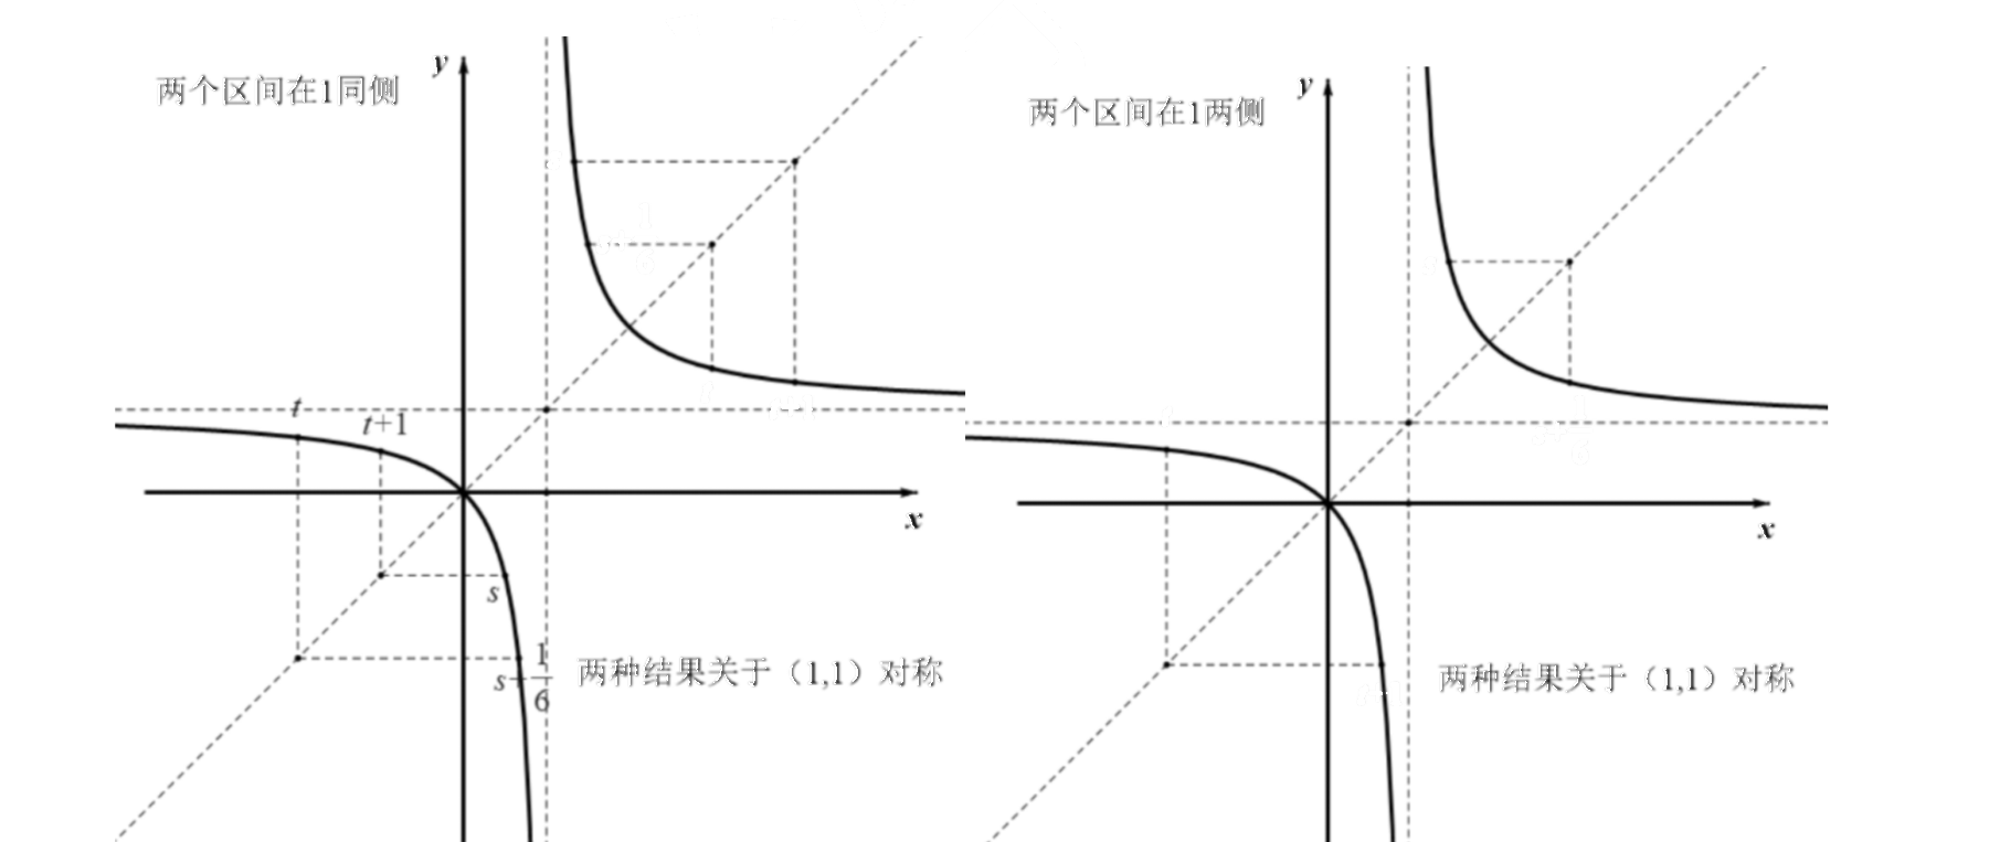
\includegraphics[width=0.92\textwidth]{figures/gao115_q10.png}
\end{center}
\solend
\fi

\end{enumerate}

\bigsec{二、选择题}

\begin{enumerate}
\setcounter{enumi}{10}

\item “对任意有理数 $x$ 都有 $x^2\neq2$”的否定形式是\mbox{（\quad）}% 原卷把答案“$B$”印在题干括号内、无【解析】

\keepwithprev
A. 存在有理数 $x$ 使得 $x^2\neq2$\qquad\qquad B. 存在有理数 $x$ 使得 $x^2=2$

C. 存在无理数 $x$ 使得 $x^2\neq2$\qquad\qquad D. 存在无理数 $x$ 使得 $x^2=2$

\ifanswer
\ans{$B$}
\fi

\item 已知 $a$、$b$ 都是实数，那么“$a^3>b^3$”是“$a^2>b^2$”的\mbox{（\quad）}

\keepwithprev
A. 充分不必要条件\qquad\qquad B. 必要不充分条件

C. 充要条件\qquad\qquad\qquad D. 既不充分也不必要条件

\ifanswer
\solbegin
\step{因为 $a^3>b^3$ 等价于 $a>b$，}
\step{由于 $a$、$b$ 正负不定，所以由 $a>b$ 不能得到 $a^2>b^2$，}
\step{由 $a^2>b^2$ 也不能得到 $a>b$，}
\step{因此“$a^3>b^3$”是“$a^2>b^2$”的既不充分也不必要条件. 故选 $D$.}
\solend
\fi

\item 定义集合运算 $A-B=\{x\mid x\in A$ 且 $x\notin B\}$，将 $A\triangle B=(A-B)\cup(B-A)$ 称为集合 $A$ 与集合 $B$ 的对称差.

命题一：$A\triangle B=B\triangle A$；

命题二：$A\triangle\varnothing=A$；

命题三：$A\cap(B\triangle C)=(A\cap B)\triangle(A\cap C)$；

命题四：$A\cup(B\triangle C)=(A\cup B)\triangle(A\cup C)$；

其中正确命题的个数是\mbox{（\quad）}

\keepwithprev
A. $1$\qquad\qquad B. $2$\qquad\qquad C. $3$\qquad\qquad D. $4$

\ifanswer
\solbegin
\step{对于①，$B\triangle A=(B-A)\cup(A-B)=(A-B)\cup(B-A)=A\triangle B$，①对；}
\step{对于②，$A-B=\{x\mid x\in A$ 且 $x\notin B\}=\{x\mid x\in A$ 且 $x\notin(A\cap B)\}$}
\step{$=A-(A\cap B)$，则 $A\triangle\varnothing=(A-\varnothing)\cup(\varnothing-A)=A\cup\varnothing=A$，②对；}
\step{对于③，$A\cap(B\triangle C)=A\cap(B\cup C-B\cap C)=A\cap(B\cup C)-A\cap(B\cap C)$}
\step{$=(A\cap B)\cup(A\cap C)-(A\cap B)\cap(A\cap C)=(A\cap B)\triangle(A\cap C)$，③对；}
\step{对于④，如图所示：}
\begin{center}
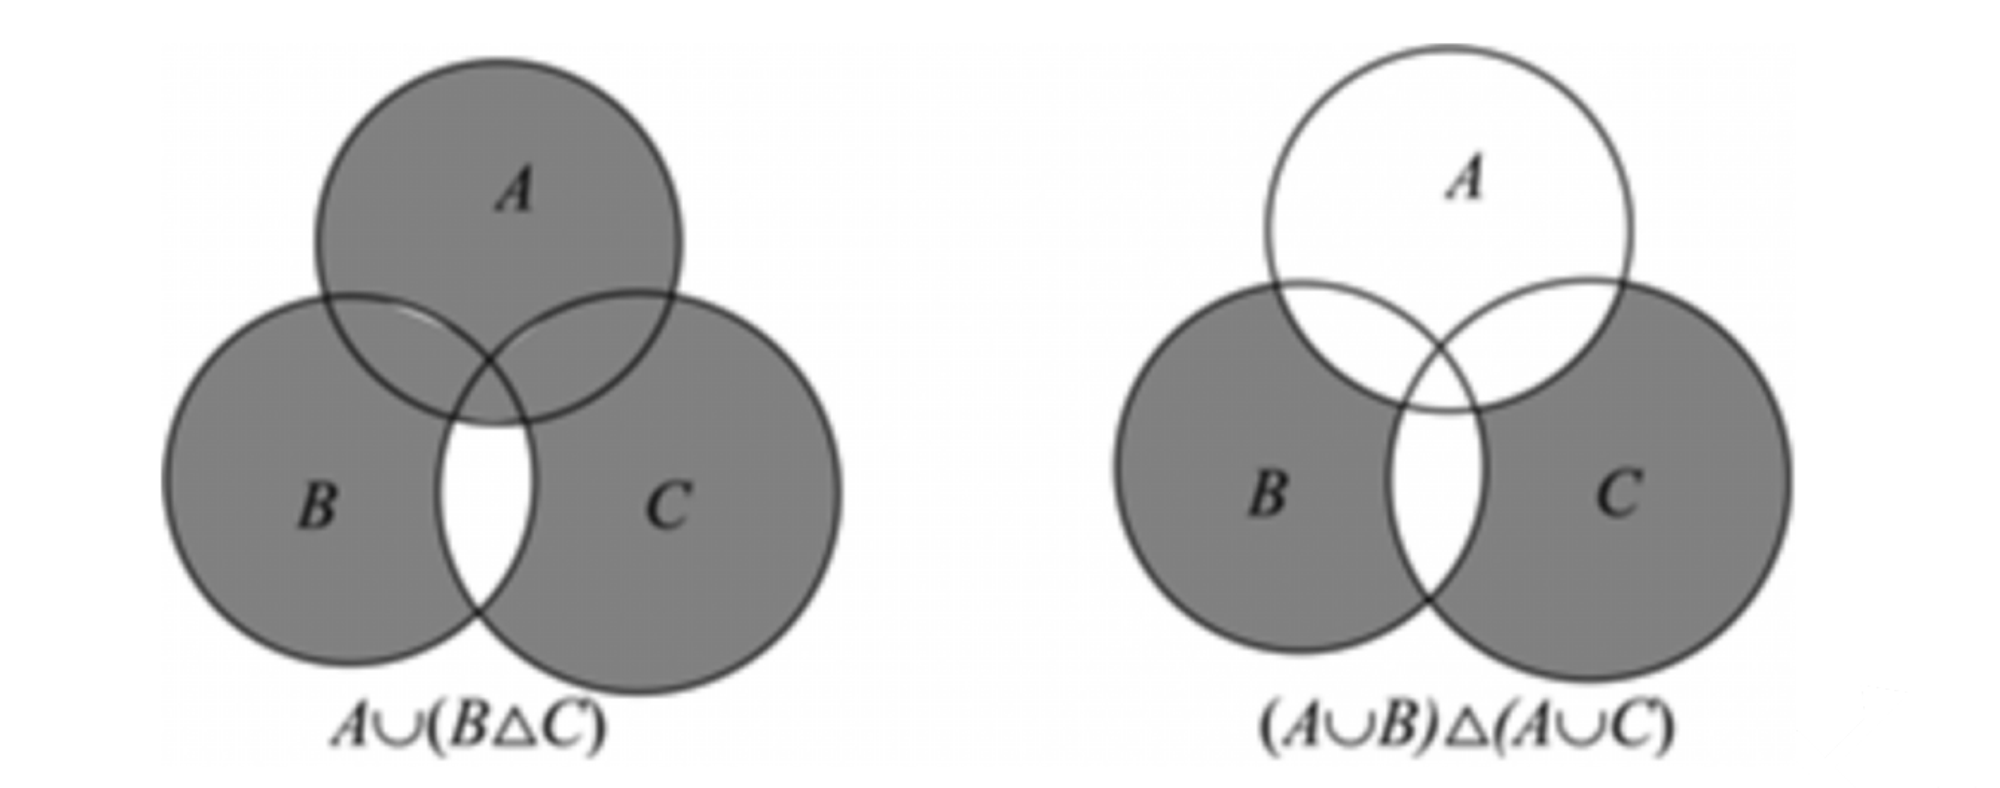
\includegraphics[width=0.85\textwidth]{figures/gao115_q13.png}
\end{center}
\step{所以 $A\cup(B\triangle C)\neq(A\cup B)\triangle(A\cup C)$，④错.}
\step{故选 $C$.}
\solend
\fi

\item 设 $a$、$b$、$c$、$p$ 为实数，若同时满足不等式 $ax^2+bx+c>0$、$bx^2+cx+a>0$ 与 $cx^2+ax+b>0$ 的全体实数 $x$ 所组成的集合等于 $(p,+\infty)$，则关于结论：① $a$、$b$、$c$ 至少有一个为 $0$；② $p=0$. 下列判断中正确的是\mbox{（\quad）}

\keepwithprev
A. ①和②都正确\qquad B. ①和②都错误\qquad C. ①正确，②错误\qquad D. ①错误，②正确

\ifanswer
\solbegin
\step{若同时满足不等式 $ax^2+bx+c>0$、$bx^2+cx+a>0$ 与 $cx^2+ax+b>0$ 的}
\step{全体实数 $x$ 所组成的集合等于 $(p,+\infty)$，必有 $a$,$b$,$c\geqslant0$，}
\step{不妨假设 $a$、$b$、$c$ 没有一个为 $0$，}
\step{则三个不等式均为开口向上的二次函数大于 $0$ 的部分，}
\step{解集的交集应为 $(-\infty,m)\cup(n,+\infty)$ 的形式，矛盾，}
\step{所以 $a$、$b$、$c$ 至少有一个为 $0$，故①正确：}
\step{不妨设 $a=0$，则 $b$,$c\geqslant0$，则不等式组化为 $\begin{cases}bx+c>0\\bx^2+cx>0,\\cx^2+b>0\end{cases}$}
\step{所以 $\begin{cases}x>-\dfrac cb\\x<-\dfrac cb\text{或}x>0\\x\in\R\end{cases}$，取交集得 $(0,+\infty)$，故 $p=0$，故②正确：}
\step{故选 $A$.}
\solend
\fi

\end{enumerate}

\bigsec{三、解答题}

\begin{enumerate}
\setcounter{enumi}{14}

\item 已知 $a>0$，$b>0$，

（1）试比较 $\dfrac{a^2-b^2}{a^2+b^2}$ 与 $\dfrac{a-b}{a+b}$ 的大小；

（2）若 $a+b>4$，求证：$\dfrac a{b+2}$ 和 $\dfrac b{a+2}$ 中至少有一个大于 $\dfrac12$.

\ifanswer
\solbegin
\step{（1）已知 $a>0$，$b>0$，$\dfrac{a^2-b^2}{a^2+b^2}-\dfrac{a-b}{a+b}=\dfrac{2ab(a-b)}{(a^2+b^2)(a+b)}$，}
\step{当 $a>b$ 时，$a-b>0$，所以 $\dfrac{a^2-b^2}{a^2+b^2}-\dfrac{a-b}{a+b}>0$，所以 $\dfrac{a^2-b^2}{a^2+b^2}>\dfrac{a-b}{a+b}$；}
\step{当 $a=b$ 时，$a-b=0$，所以 $\dfrac{a^2-b^2}{a^2+b^2}-\dfrac{a-b}{a+b}=0$，所以 $\dfrac{a^2-b^2}{a^2+b^2}=\dfrac{a-b}{a+b}$；}
\step{当 $a<b$ 时，$a-b<0$，所以 $\dfrac{a^2-b^2}{a^2+b^2}-\dfrac{a-b}{a+b}<0$，所以 $\dfrac{a^2-b^2}{a^2+b^2}<\dfrac{a-b}{a+b}$；}
\step{（2）假设 $\dfrac a{b+2}$ 和 $\dfrac b{a+2}$ 中都不大于 $\dfrac12$，即 $\dfrac b{a+2}\leqslant\dfrac12$，$\dfrac a{b+2}\leqslant\dfrac12$，}
\step{因为 $a>0$，$b>0$，所以 $a+2>0$，$b+2>0$，}
\step{所以 $2b\leqslant a+2$，$2a\leqslant b+2$，}
\step{两式相加得 $2a+2b\leqslant a+2+b+2=a+b+4$，即 $a+b\leqslant4$，}
\step{与已知 $a+b>4$ 矛盾，所以假设错误，}
\step{故 $\dfrac a{b+2}$ 和 $\dfrac b{a+2}$ 中至少有一个大于 $\dfrac12$.}
\solend
\fi

\item 某企业原有 $200$ 名科技人员，年人均工资 $a$ 万元($a>0$). 现加大对某芯片研发力度，该企业把原有 $200$ 名科技人员调整成技术人员和研发人员，其中技术人员 $x$ 名($x\in\N$ 且 $40\leqslant x\leqslant80$). 调整后，研发人员的年人均工资比调整前增加了 $(2x)\%$，技术人员的年人均工资为 $a\left(m-\dfrac x{10}\right)$万元.

（1）若要使调整后研发人员的年总工资不低于调整前 $200$ 名科技人员年总工资的 $1.5$ 倍，求调整后的技术人员最少有多少人？

（2）为了激励研发人员的工作热情和保持技术人员的工作积极性，企业决定在工资方面要同时满足以下两个条件：

①研发人员的年总工资始终不低于技术人员的年总工资；

②技术人员的年人均工资始终不低于调整前 $200$ 名科技人员的年人均工资.

请问是否存在这样的实数 $m$？若存在，求出 $m$ 的范围；若不存在，说明理由.

\ifanswer
\solbegin
\step{（1）由题意得调整后研发人员的年人均工资为 $[1+(2x)\%]a$ 万元，}
\step{那么 $(200-x)[1+(2x)\%]a\geqslant1.5\times200a$ ($a>0$)，}
\step{化简得 $x^2-150x+5000\leqslant0$，解得 $50\leqslant x\leqslant100$，}
\step{由于 $x\in\N$ 且 $40\leqslant x\leqslant80$，因此 $50\leqslant x\leqslant80$，}
\step{因此调整后的技术人员的人数最少为 $50$ 人；}
\step{（2）假设存在实数 $m$，使得技术人员在已知范围内调整后，满足以上两个条件，}
\step{由条件①得 $(200-x)[1+(2x)\%]a\geqslant x\left(m-\dfrac x{10}\right)a$，}
\step{整理得 $m\leqslant\dfrac{200}{x}+\dfrac{2x}{25}+3$；}
\step{因为 $\dfrac{200}{x}+\dfrac{2x}{25}+3\geqslant2\sqrt{\dfrac{200}{x}\cdot\dfrac{2x}{25}}+3=11$，}
\step{当且仅当 $\dfrac{200}{x}=\dfrac{2x}{25}$，即 $x=50$ 时取等号，因此 $m\leqslant11$，}
\step{由条件②得 $a\left(m-\dfrac x{10}\right)\geqslant a$，所以 $m\geqslant\dfrac x{10}+1$；}
\step{又由于 $40\leqslant x\leqslant80$，因此 $m\geqslant9$.}
\step{因此 $m\in[9,11]$.}
\solend
\fi

\item 已知 $a\in\R$，记 $f(x)=ax^2-(a+2)x+2$.

（1）若 $f(x)<3-2x$ 对于一切 $x\in\R$ 恒成立，求实数 $a$ 的取值范围；

（2）求关于 $x$ 不等式 $f(x)\geqslant0$ 的解集；

（3）若存在 $m\in\R$ 使关于 $x$ 的方程 $ax^2-(a+2)\lvert x\rvert+2=\lvert m+2\rvert+\lvert m-1\rvert$ 有四个不同的实根，求实数 $a$ 的取值范围.

\ifanswer
\solbegin
\step{（1）由 $f(x)<3-2x$ 对于一切 $x\in\R$ 恒成立，}
\step{得 $ax^2-ax-1<0$ 对于一切 $x\in\R$ 恒成立，}
\step{当 $a=0$ 时，原式可化为 $-1<0$，恒成立，符合条件；}
\step{当 $a\neq0$ 时，需满足 $\begin{cases}a<0\\\Delta=a^2+4a<0\end{cases}$，解得 $-4<a<0$；}
\step{综上，实数 $a$ 的取值范围是 $(-4,0]$；}
\step{（2）$f(x)\geqslant0$，即 $(ax-2)(x-1)\geqslant0$，}
\step{当 $a=0$ 时，原式化为 $-2x+2\geqslant0$，解集为 $\{x\mid x\leqslant1\}$；}
\step{当 $a>0$ 时，若 $a=2$，原式化为 $2(x-1)^2\geqslant0$，解集为 $\R$；}
\step{若 $0<a<2$，$\dfrac2a>1$，解集为 $\{x\mid x\leqslant1$ 或 $x\geqslant\dfrac2a\}$；}
\step{若 $a>2$，$\dfrac2a<1$，解集为 $\{x\mid x\leqslant\dfrac2a$ 或 $x\geqslant1\}$；}
\step{当 $a<0$ 时，$\dfrac2a<1$，解集为 $\left\{x\,\middle\vert\,\dfrac2a\leqslant x\leqslant1\right\}$；}
\step{综上，当 $a<0$ 时，不等式解集为 $\left\{x\,\middle\vert\,\dfrac2a\leqslant x\leqslant1\right\}$；}
\step{当 $a=0$ 时，不等式解集为 $\{x\mid x\leqslant1\}$；}
\step{当 $0<a<2$ 时，不等式解集为 $\{x\mid x\leqslant1$ 或 $x\geqslant\dfrac2a\}$；}
\step{当 $a=2$ 时，不等式解集为 $\R$；}
\step{当 $a>2$ 时，不等式解集为 $\{x\mid x\leqslant\dfrac2a$ 或 $x\geqslant1\}$；}
\step{（3）由绝对值三角不等式得 $\lvert m+2\rvert+\lvert m-1\rvert\geqslant\lvert(m+2)-(m-1)\rvert=3$，}
\step{即右侧取值范围为 $[3,+\infty)$，}
\step{令 $t=\lvert x\rvert\geqslant0$，原方程转化为 $at^2-(a+2)t+2=k$，$k\in[3,+\infty)$，}
\step{若原方程有四个不同实根，}
\step{需存在 $k\geqslant3$，使得方程 $at^2-(a+2)t+2-k=0$ 有两个不同正实根，}
\step{当 $a\geqslant0$ 时，方程的两根之积为 $\dfrac{2-k}{a}$，}
\step{因为 $k\geqslant3$，所以 $2-k\leqslant-1<0$，两根一正一负，}
\step{最多只有一个正根，对应最多两个 $x$ 根，不符合要求；}
\step{当 $a<0$ 时，两根之积为正，}
\step{要两个根都为正，需要两根之和 $\dfrac{a+2}{a}>0$，解得 $a<-2$，}
\step{再要求存在 $k\geqslant3$ 使得判别式大于 $0$，}
\step{即 $\triangle=(a+2)^2-4a(2-k)>0$ 在 $k\in[3,+\infty)$ 上有解，}
\step{即 $(a-2)^2+4ak>0$ 在 $k\in[3,+\infty)$ 上有解，}
\step{由 $a<0$，得 $(a-2)^2+12a>0$，}
\step{即 $a^2+8a+4>0$，结合 $a<-2$ 解得 $a<-4-2\sqrt3$，}
\step{故实数 $a$ 的取值范围是 $(-\infty,-4-2\sqrt3)$.}
\solend
\fi

\item 设 $A=\{x_1,x_2,\cdots,x_n\}(n\geqslant2,n\in\N)$，且 $x_1,x_2,\cdots,x_n$ 均为正整数，若对于 $A$ 中任意两个元素 $a,b$，当 $a>b$ 时，都有 $\dfrac{b^2}{a-b}\in A$，则称 $A$ 为“$n$ 元好集”.

（1）判断 $\{2,4,6\}$ 是否为“三元好集”，并说明理由；

（2）若集合 $M$ 为“二元好集”，且 $M$ 中所有元素之积小于 $2026$，求所有满足条件的集合 $M$ 的个数；

（3）设 $k\geqslant3,k\in\N$，是否存在“$k$ 元好集”，若存在，求出所有满足条件的“$k$ 元好集”，若不存在，请说明理由.

\ifanswer
\solbegin
\step{（1）取 $a=6,b=2$，则 $\dfrac{b^2}{a-b}=\dfrac44=1\notin\{2,4,6\}$，所以该集合不是三元好集.}
\step{（2）设 $M=\{b,a\}$，其中 $a>b$ 且均为正整数，则 $\dfrac{b^2}{a-b}$ 等于 $a$ 或 $b$.}
\step{若 $\dfrac{b^2}{a-b}=a$，则 $a^2-ab-b^2=0$，从而 $\dfrac ab=\dfrac{1+\sqrt5}{2}$，与 $\dfrac ab$ 为有理数矛盾.}
\step{若 $\dfrac{b^2}{a-b}=b$，则 $a=2b$；}
\step{反之，任意正整数 $b$ 对应的 $\{b,2b\}$ 均为二元好集.}
\step{由元素之积小于 $2026$，得 $2b^2<2026\Leftrightarrow b^2<1013$.}
\step{因为 $31^2=961<1013<1024=32^2$，所以 $b=1,2,\cdots,31$，}
\step{对应 $31$ 个不同的集合.}
\step{（3）假设存在 $k\geqslant3$ 的 $k$ 元好集 $A$，将其元素从小到大排列，}
\step{记最小元素为 $u$，次小元素为 $v$，最大元素为 $w$，则 $0<u<v<w$.}
\step{由 $\dfrac{u^2}{w-u}\in A$，该数不小于 $u$，得 $\dfrac{u^2}{w-u}\geqslant u\Rightarrow w\leqslant2u$.}
\step{又由 $\dfrac{u^2}{v-u}$,$\dfrac{v^2}{w-v}\in A$，这两个数均不超过 $w$，}
\step{得 $\dfrac{u^2}{v-u}\leqslant w$,$\dfrac{v^2}{w-v}\leqslant w$，}
\step{分母均为正，分别去分母后相加，}
\step{得 $u^2+v^2\leqslant w(v-u)+w(w-v)=w(w-u)\leqslant2u^2$，}
\step{于是 $v^2\leqslant u^2$，与 $v>u>0$ 矛盾，所以不存在 $k\geqslant3$ 的 $k$ 元好集.}
\solend
\fi

\end{enumerate}

\end{document}
"
%
% 原始材料：微信公众号“魔都数学加油站”文章，作者破晓，2026-11-06 17:58 发布；
% 连载“27学年高一115”，原文标题“27学年高一115——2026-2027年上海市复旦附中高一上10月阶段练习”；
% 原文链接：https://mp.weixin.qq.com/s/krocP0fMQQ4VM1SQEcLI2Q。
% 正文为 12 张 PNG 页（第 4、6、12 页 2560×3620，其余 4762×6735），
% 题目下印有【解析】或【答案】，为讲评版。
% 题目、解析均据原图转录；卷面红色水印及公众号页脚未录入。
%
% 卷首标题：原卷印作“2026-2027 年复旦附中高一上 10 月阶段练习”（公众号标题中的“上海市”
% 卷面标题行没有，本稿照卷面），年份区间按全稿惯例排 en dash；原卷未印副标题，本稿按题目内容
% 标为“集合与常用逻辑用语、不等式”。
%
% 与原卷的排版差异：
%   ① 原文从第 3 题起，填空题编号为 3—10、选择题为 11—14、解答题为 15—18，共 16 题，
%      本稿保留原题号（与多数卷的 3—21 不同）；
%   ② 原卷每题下直接印【解析】／【答案】，本稿按全稿惯例置于答案版；第 11 题把答案“$B$”
%      印在题干括号内且无【解析】，另提 \ans{}；其余选择题答案在解析末句“故选 …”，括号内留空；
%   ③ 原卷未印副标题，本稿按“知识模块”口径补出；
%   ④ 原卷填空横线按全稿惯例排为 \blankline[4.4em]；选择题括号排 \mbox{（\quad）}、
%      选项段前按惯例加 \keepwithprev；解答题不留作答区（原卷为讲评版，与 109—114 同）；
%   ⑤ 原卷数集排斜体 $R$／$Q$／$N$，按全稿惯例改 \R、\Q、\N。
%
% 判别式与对称差字形：原卷 $\triangle$（等边、扁）与 $\Delta$（等腰、高）两种混用，逐处照录——
%   第 7 题与第 17 题 (3) 的判别式、第 13 题的对称差 $A\triangle B$ 用 \triangle，
%   第 17 题 (1) cases 的判别式用 \Delta。
%
% 子集符号：第 4 题解析的 $(-1,3)\subset(-m,m)$ 印单线（真子集、无下划线），按 18／96
%   成例照录 \subset；第 5 题解析的 $B\subseteq A$ 印有下划线，照录 \subseteq。
%   第 3 题的补集照原卷上划线排 \overline{N}。
%
% 原卷存疑照录：第 9 题解析末行“故可能成立的是①②③”与四种情形的编号一致，照录；
%   第 10 题解析两幅函数图上另有蓝色／红色手写标注（$t$、$t+1$、$s$、$\frac16$ 等），
%   系批改笔迹，随裁图保留、不另作正文录入；第 14 题解析的 cases 三行照原卷排；
%   第 18 题 (2) 解析“所以该集合不是三元好集”前的取例 $a=6,b=2$ 照录。
%
% 行数核对：逐题数 \step/\stepm 条数，合计 133 条（Q3：3；Q4：3；Q5：4；Q6：5；Q7：4；
% Q8：4；Q9：11；Q10：7；Q11：0；Q12：4；Q13：8；Q14：9；Q15：10；Q16：13；
% Q17：32；Q18：16），与原卷印刷行逐题相等（cases 块作一个印刷行计）。第 11 题括号内印
% 答案且无解析，提 \ans{}，不计入 \step 账；第 10、13 题解析内的插图不计入 \step 账。
%
\documentclass[a4paper,11pt]{article}
\usepackage{common}

\begin{document}

\examtitlest[3]{2026--2027 年复旦附中高一上 10 月阶段练习}{集合与常用逻辑用语、不等式}

\bigsec{一、填空题}

\begin{enumerate}
\setcounter{enumi}{2}

\item 已知集合 $M=\{x\mid 4x^2-4x-15>0\}$，$N=\left\{x\,\middle\vert\,\dfrac{x+1}{x-6}>0\right\}$，则 $M\cap\overline{N}=$\blankline[4.4em].

\ifanswer
\solbegin
\step{集合 $M=\{x\mid 4x^2-4x-15>0\}=\{x\mid x>\dfrac52$ 或 $x<-\dfrac32\}$，}
\step{$N=\left\{x\,\middle\vert\,\dfrac{x+1}{x-6}>0\right\}=\{x\mid x>6$ 或 $x<-1\}$，得 $\overline{N}=\{x\mid-1\leqslant x\leqslant6\}$，}
\step{故 $M\cap\overline{N}=\left\{x\,\middle\vert\,\dfrac52<x\leqslant6\right\}$.}
\solend
\fi

\item 已知 $m>0$，不等式 $\lvert x\rvert<m$ 成立的一个充分不必要条件是 $-1<x<3$，则 $m$ 的取值范围是\blankline[4.4em].

\ifanswer
\solbegin
\step{不等式 $-m<x<m$ 成立的一个充分不必要条件是 $-1<x<3$，}
\step{由题意得 $(-1,3)\subset(-m,m)$，则 $m\geqslant3$，此时 $-m\leqslant-3<-1$，}% 原卷印单线 \subset，照录
\step{所以 $m$ 的取值范围是 $\{m\mid m\geqslant3\}$.}
\solend
\fi

\item 已知集合 $A=\{1,2\}$，集合 $B=\{x\mid ax=6\}$，若 $A\cup B=A$，则 $a$ 的所有取值构成的集合为\blankline[4.4em].

\ifanswer
\solbegin
\step{因为 $A\cup B=A$，所以 $B\subseteq A$，}
\step{当 $a=0$ 时，$B=\varnothing$，满足 $B\subseteq A$；}
\step{当 $a\neq0$ 时，$B=\left\{\dfrac6a\right\}$，则 $\dfrac6a=1$ 或 $\dfrac6a=2$，解得 $a=6$ 或 $a=3$，}
\step{综上所述，$a$ 的所有取值构成的集合为 $\{0,3,6\}$.}
\solend
\fi

\item 若关于 $x$ 的不等式 $ax^2+bx+c>0$ 的解集为 $(-3,2)$，则不等式 $ax^2+(a+b)x+c-2a>0$ 的解集为\blankline[4.4em].

\ifanswer
\solbegin
\step{由 $ax^2+bx+c>0$ 的解集为 $(-3,2)$ 得 $a<0$，}
\step{且 $ax^2+bx+c=0$ 时 $x_1=-3$，$x_2=2$，}
\step{得 $-3+2=-\dfrac ba$，即 $b=a$，$-3\times2=\dfrac ca$，即 $c=-6a$，}
\step{代入 $ax^2+(a+b)x+c-2a>0$ 得 $ax^2+2ax-8a>0$ 化简得 $x^2+2x-8<0$，}
\step{解得 $-4<x<2$，故解集为 $(-4,2)$.}
\solend
\fi

\item 已知关于 $x$ 的方程 $x^2-2x+m=0$ 的两个实数根分别为 $x_1$，$x_2$. 若 $x_1^2x_2^2+x_1^2+x_2^2=7$，则实数 $m$ 的值为\blankline[4.4em].

\ifanswer
\solbegin
\step{由韦达定理得 $x_1+x_2=2$，$x_1x_2=m$，}
\step{$x_1^2x_2^2+x_1^2+x_2^2=(x_1x_2)^2+(x_1+x_2)^2-2x_1x_2=m^2+4-2m$，}
\step{由 $m^2+4-2m=7$，得 $m^2-2m-3=0$，解得 $m=3$ 或 $m=-1$，}
\step{方程有两个实数根，故 $\triangle=4-4m\geqslant0$，即 $m\leqslant1$，所以 $m=-1$.}
\solend
\fi

\item 已知 $x>1$，若 $x^2-xy+y=0$，则 $x+y$ 的最小值是\blankline[4.4em].

\ifanswer
\solbegin
\step{由于 $x^2-xy+y=0$，则 $y=\dfrac{x^2}{x-1}>0$，}
\step{则 $x+y=x+\dfrac{x^2}{x-1}=\dfrac{2x^2-x}{x-1}=\dfrac{2(x-1)^2+3(x-1)+1}{x-1}$}
\step{$=2(x-1)+\dfrac1{x-1}+3\geqslant2\sqrt{2(x-1)\cdot\dfrac1{x-1}}+3=2\sqrt2+3$，}
\step{当且仅当 $x=1+\dfrac{\sqrt2}{2}$ 时取等号，故最小值是 $2\sqrt2+3$.}
\solend
\fi

\item 若集合 $A=B_1\cup B_2\cup\cdots\cup B_n$，其中 $B_1$、$B_2$、$\cdots$、$B_n$ 为非空集合，$B_i\cap B_j=\varnothing$，$1\leqslant i<j\leqslant n$，则称集合 $\{B_1,B_2,\cdots,B_n\}$ 为集合 $A$ 的一个 $n$ 划分. 例如：集合 $\{\{1,2\},\{3\}\}$，$\{\{1,3\},\{2\}\}$，$\{\{2,3\},\{1\}\}$ 均为集合 $\{1,2,3\}$ 的一个 $2$ 划分. 设 $\{B_1,B_2\}$ 为有理数集 $\Q$ 的一个 $2$ 划分，且满足对任意 $x\in B_1$，任意 $y\in B_2$，都有 $x<y$. 则对于 $B_1$、$B_2$ 有：

① $B_1$ 中的元素存在最大值，$B_2$ 中的元素不存在最小值；

② $B_1$ 中的元素不存在最大值，$B_2$ 中的元素存在最小值；

③ $B_1$ 中的元素不存在最大值，$B_2$ 中的元素不存在最小值；

④ $B_1$ 中的元素存在最大值，$B_2$ 中的元素存在最小值；

对于以上四种情况，可能成立的序号有\blankline[4.4em].

\ifanswer
\solbegin
\step{对于①，$B_1=\{x\in\Q\mid x\leqslant2\}$，$B_2=\{x\in\Q\mid x>2\}$，①可能成立；}
\step{对于②，$B_1=\{x\in\Q\mid x<2\}$，$B_2=\{x\in\Q\mid x\geqslant2\}$，②可能成立；}
\step{对于③，$B_1=\{x\in\Q\mid x<\pi\}$，$B_2=\{x\in\Q\mid x>\pi\}$，③可能成立；}
\step{对于④，假设④成立，}
\step{不妨设 $B_1$ 中的元素的最大值为 $s$，$B_2$ 中的元素的最小值为 $t$，}
\step{由题意得 $s<t$，所以 $s<\dfrac{s+t}{2}<t$，}
\step{因为 $s$ 为 $B_1$ 中的元素的最大值，所以 $\dfrac{s+t}{2}\notin B_1$，}
\step{因为 $t$ 为 $B_2$ 中的元素的最小值，所以 $\dfrac{s+t}{2}\notin B_2$，}
\step{又 $B_1\cup B_2=\Q$，所以 $\dfrac{s+t}{2}\notin\Q$，与 $\dfrac{s+t}{2}\in\Q$ 矛盾，}
\step{所以假设不成立，即④不可能成立.}
\step{故可能成立的是①②③.}
\solend
\fi

\item 已知集合 $A=\left[s,s+\dfrac16\right]\cup[t,t+1]$，其中 $1\notin A$ 且 $s+\dfrac16<t$，函数 $f(x)=\dfrac x{x-1}$，且对任意 $a\in A$，都有 $f(a)\in A$，则 $t$ 的值是\blankline[4.4em].

\ifanswer
\solbegin
\step{若 $\left[s,s+\dfrac16\right]$,$[t,t+1]$ 在 $f(x)=\dfrac x{x-1}$ 图像的同侧，}
\step{则点 $\left(t,s+\dfrac16\right)$,$(t+1,s)$ 在 $f(x)=\dfrac x{x-1}$ 的图像上，}
\step{所以 $\dfrac t{t-1}=\dfrac{t+1}{t}+\dfrac16$，解得 $t=-2$ 或 $t=3$，检验得 $t=3$；}
\step{若 $\left[s,s+\dfrac16\right]$,$[t,t+1]$ 在 $f(x)=\dfrac x{x-1}$ 图像的两侧，}
\step{则点 $(t,t+1)$ 在 $f(x)=\dfrac x{x-1}$ 的图像上，}
\step{所以 $t+1=\dfrac t{t-1}$，解得 $t=\dfrac{1\pm\sqrt5}{2}$，检验得 $t=\dfrac{1+\sqrt5}{2}$，}
\step{综上，$t=\dfrac{1+\sqrt5}{2}$ 或 $t=3$.}
\begin{center}
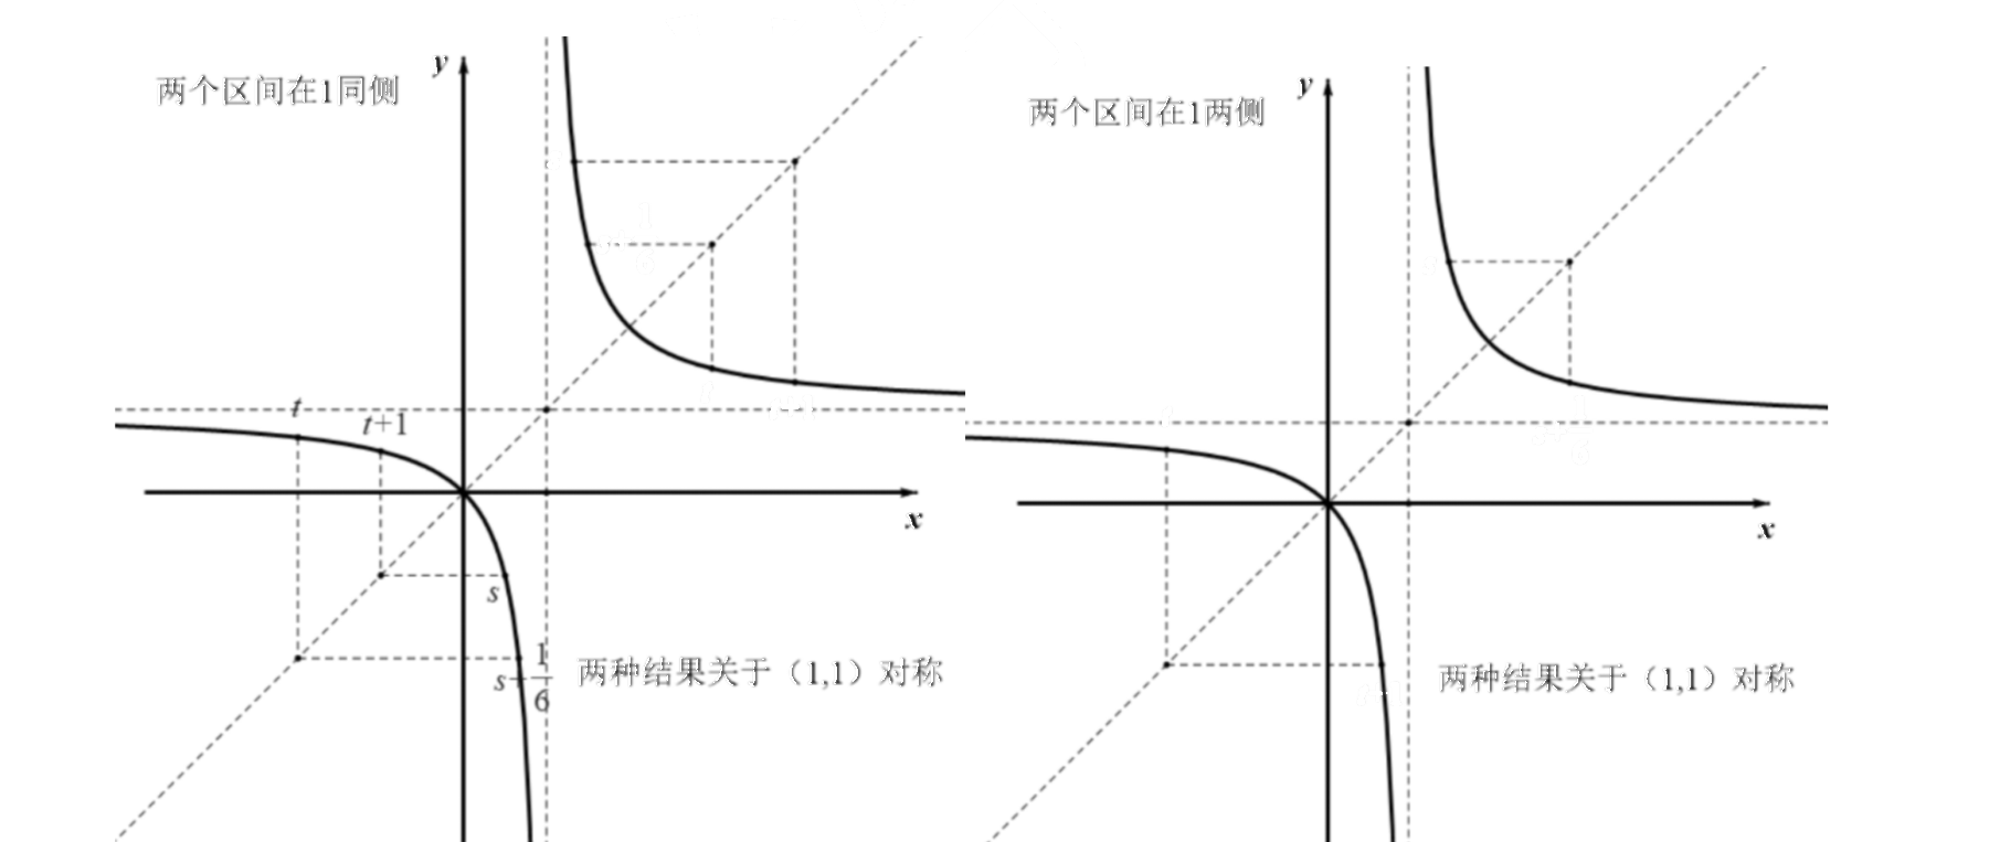
\includegraphics[width=0.92\textwidth]{figures/gao115_q10.png}
\end{center}
\solend
\fi

\end{enumerate}

\bigsec{二、选择题}

\begin{enumerate}
\setcounter{enumi}{10}

\item “对任意有理数 $x$ 都有 $x^2\neq2$”的否定形式是\mbox{（\quad）}% 原卷把答案“$B$”印在题干括号内、无【解析】

\keepwithprev
A. 存在有理数 $x$ 使得 $x^2\neq2$\qquad\qquad B. 存在有理数 $x$ 使得 $x^2=2$

C. 存在无理数 $x$ 使得 $x^2\neq2$\qquad\qquad D. 存在无理数 $x$ 使得 $x^2=2$

\ifanswer
\ans{$B$}
\fi

\item 已知 $a$、$b$ 都是实数，那么“$a^3>b^3$”是“$a^2>b^2$”的\mbox{（\quad）}

\keepwithprev
A. 充分不必要条件\qquad\qquad B. 必要不充分条件

C. 充要条件\qquad\qquad\qquad D. 既不充分也不必要条件

\ifanswer
\solbegin
\step{因为 $a^3>b^3$ 等价于 $a>b$，}
\step{由于 $a$、$b$ 正负不定，所以由 $a>b$ 不能得到 $a^2>b^2$，}
\step{由 $a^2>b^2$ 也不能得到 $a>b$，}
\step{因此“$a^3>b^3$”是“$a^2>b^2$”的既不充分也不必要条件. 故选 $D$.}
\solend
\fi

\item 定义集合运算 $A-B=\{x\mid x\in A$ 且 $x\notin B\}$，将 $A\triangle B=(A-B)\cup(B-A)$ 称为集合 $A$ 与集合 $B$ 的对称差.

命题一：$A\triangle B=B\triangle A$；

命题二：$A\triangle\varnothing=A$；

命题三：$A\cap(B\triangle C)=(A\cap B)\triangle(A\cap C)$；

命题四：$A\cup(B\triangle C)=(A\cup B)\triangle(A\cup C)$；

其中正确命题的个数是\mbox{（\quad）}

\keepwithprev
A. $1$\qquad\qquad B. $2$\qquad\qquad C. $3$\qquad\qquad D. $4$

\ifanswer
\solbegin
\step{对于①，$B\triangle A=(B-A)\cup(A-B)=(A-B)\cup(B-A)=A\triangle B$，①对；}
\step{对于②，$A-B=\{x\mid x\in A$ 且 $x\notin B\}=\{x\mid x\in A$ 且 $x\notin(A\cap B)\}$}
\step{$=A-(A\cap B)$，则 $A\triangle\varnothing=(A-\varnothing)\cup(\varnothing-A)=A\cup\varnothing=A$，②对；}
\step{对于③，$A\cap(B\triangle C)=A\cap(B\cup C-B\cap C)=A\cap(B\cup C)-A\cap(B\cap C)$}
\step{$=(A\cap B)\cup(A\cap C)-(A\cap B)\cap(A\cap C)=(A\cap B)\triangle(A\cap C)$，③对；}
\step{对于④，如图所示：}
\begin{center}
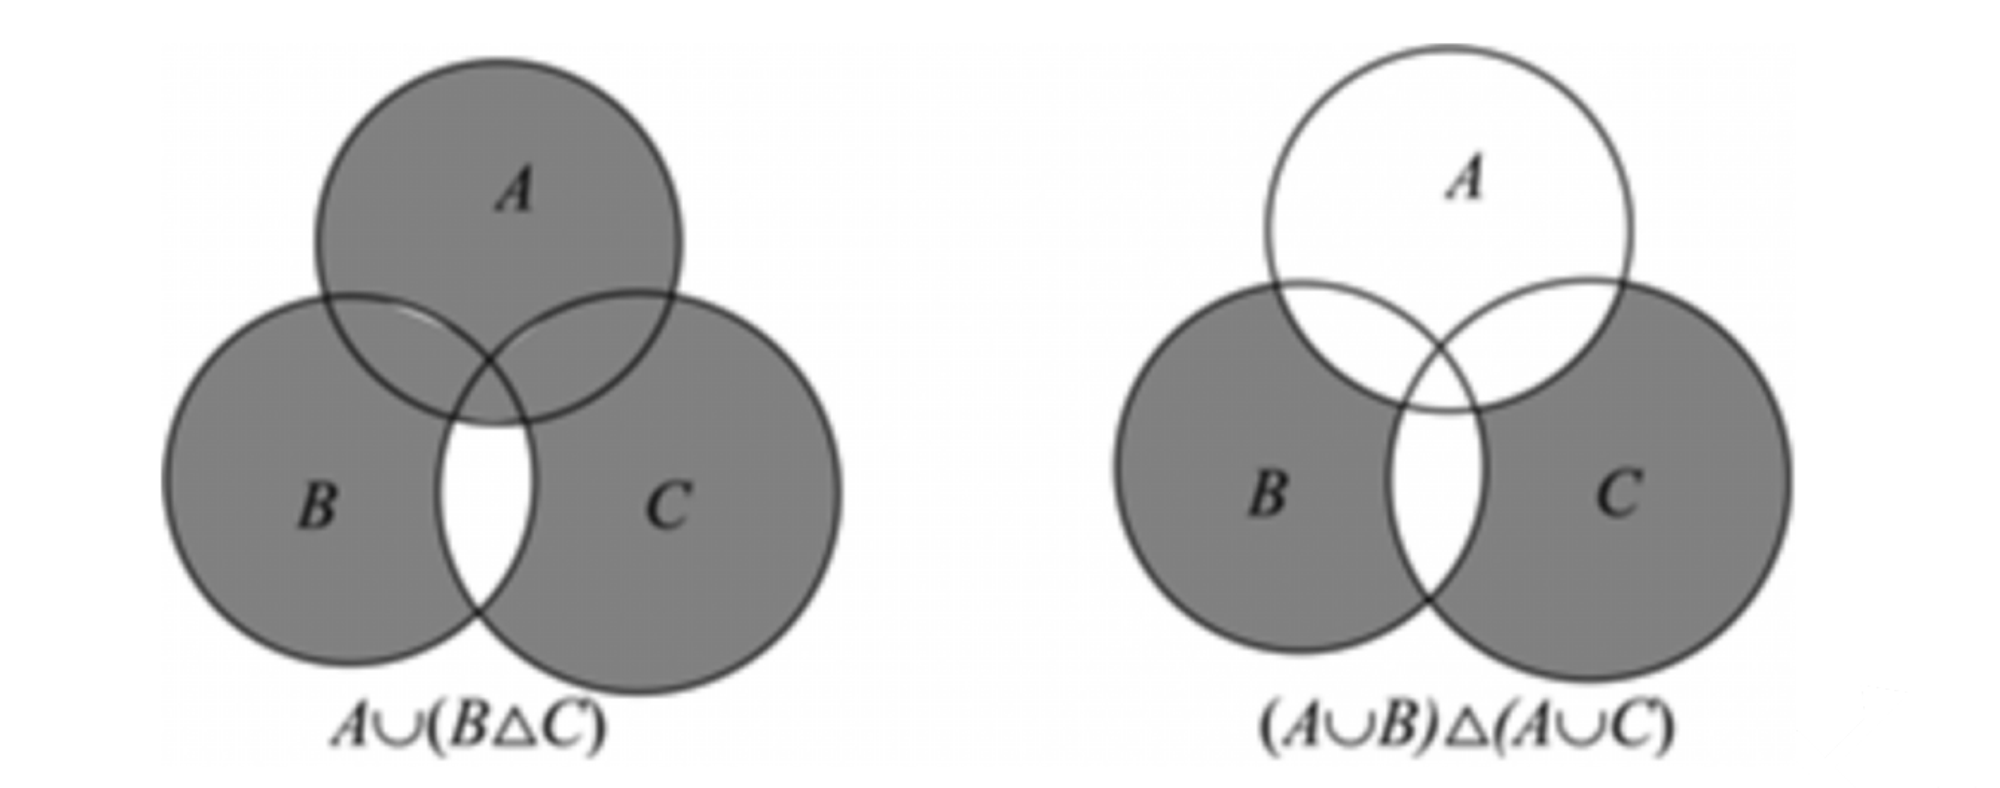
\includegraphics[width=0.85\textwidth]{figures/gao115_q13.png}
\end{center}
\step{所以 $A\cup(B\triangle C)\neq(A\cup B)\triangle(A\cup C)$，④错.}
\step{故选 $C$.}
\solend
\fi

\item 设 $a$、$b$、$c$、$p$ 为实数，若同时满足不等式 $ax^2+bx+c>0$、$bx^2+cx+a>0$ 与 $cx^2+ax+b>0$ 的全体实数 $x$ 所组成的集合等于 $(p,+\infty)$，则关于结论：① $a$、$b$、$c$ 至少有一个为 $0$；② $p=0$. 下列判断中正确的是\mbox{（\quad）}

\keepwithprev
A. ①和②都正确\qquad B. ①和②都错误\qquad C. ①正确，②错误\qquad D. ①错误，②正确

\ifanswer
\solbegin
\step{若同时满足不等式 $ax^2+bx+c>0$、$bx^2+cx+a>0$ 与 $cx^2+ax+b>0$ 的}
\step{全体实数 $x$ 所组成的集合等于 $(p,+\infty)$，必有 $a$,$b$,$c\geqslant0$，}
\step{不妨假设 $a$、$b$、$c$ 没有一个为 $0$，}
\step{则三个不等式均为开口向上的二次函数大于 $0$ 的部分，}
\step{解集的交集应为 $(-\infty,m)\cup(n,+\infty)$ 的形式，矛盾，}
\step{所以 $a$、$b$、$c$ 至少有一个为 $0$，故①正确：}
\step{不妨设 $a=0$，则 $b$,$c\geqslant0$，则不等式组化为 $\begin{cases}bx+c>0\\bx^2+cx>0,\\cx^2+b>0\end{cases}$}
\step{所以 $\begin{cases}x>-\dfrac cb\\x<-\dfrac cb\text{或}x>0\\x\in\R\end{cases}$，取交集得 $(0,+\infty)$，故 $p=0$，故②正确：}
\step{故选 $A$.}
\solend
\fi

\end{enumerate}

\bigsec{三、解答题}

\begin{enumerate}
\setcounter{enumi}{14}

\item 已知 $a>0$，$b>0$，

（1）试比较 $\dfrac{a^2-b^2}{a^2+b^2}$ 与 $\dfrac{a-b}{a+b}$ 的大小；

（2）若 $a+b>4$，求证：$\dfrac a{b+2}$ 和 $\dfrac b{a+2}$ 中至少有一个大于 $\dfrac12$.

\ifanswer
\solbegin
\step{（1）已知 $a>0$，$b>0$，$\dfrac{a^2-b^2}{a^2+b^2}-\dfrac{a-b}{a+b}=\dfrac{2ab(a-b)}{(a^2+b^2)(a+b)}$，}
\step{当 $a>b$ 时，$a-b>0$，所以 $\dfrac{a^2-b^2}{a^2+b^2}-\dfrac{a-b}{a+b}>0$，所以 $\dfrac{a^2-b^2}{a^2+b^2}>\dfrac{a-b}{a+b}$；}
\step{当 $a=b$ 时，$a-b=0$，所以 $\dfrac{a^2-b^2}{a^2+b^2}-\dfrac{a-b}{a+b}=0$，所以 $\dfrac{a^2-b^2}{a^2+b^2}=\dfrac{a-b}{a+b}$；}
\step{当 $a<b$ 时，$a-b<0$，所以 $\dfrac{a^2-b^2}{a^2+b^2}-\dfrac{a-b}{a+b}<0$，所以 $\dfrac{a^2-b^2}{a^2+b^2}<\dfrac{a-b}{a+b}$；}
\step{（2）假设 $\dfrac a{b+2}$ 和 $\dfrac b{a+2}$ 中都不大于 $\dfrac12$，即 $\dfrac b{a+2}\leqslant\dfrac12$，$\dfrac a{b+2}\leqslant\dfrac12$，}
\step{因为 $a>0$，$b>0$，所以 $a+2>0$，$b+2>0$，}
\step{所以 $2b\leqslant a+2$，$2a\leqslant b+2$，}
\step{两式相加得 $2a+2b\leqslant a+2+b+2=a+b+4$，即 $a+b\leqslant4$，}
\step{与已知 $a+b>4$ 矛盾，所以假设错误，}
\step{故 $\dfrac a{b+2}$ 和 $\dfrac b{a+2}$ 中至少有一个大于 $\dfrac12$.}
\solend
\fi

\item 某企业原有 $200$ 名科技人员，年人均工资 $a$ 万元($a>0$). 现加大对某芯片研发力度，该企业把原有 $200$ 名科技人员调整成技术人员和研发人员，其中技术人员 $x$ 名($x\in\N$ 且 $40\leqslant x\leqslant80$). 调整后，研发人员的年人均工资比调整前增加了 $(2x)\%$，技术人员的年人均工资为 $a\left(m-\dfrac x{10}\right)$万元.

（1）若要使调整后研发人员的年总工资不低于调整前 $200$ 名科技人员年总工资的 $1.5$ 倍，求调整后的技术人员最少有多少人？

（2）为了激励研发人员的工作热情和保持技术人员的工作积极性，企业决定在工资方面要同时满足以下两个条件：

①研发人员的年总工资始终不低于技术人员的年总工资；

②技术人员的年人均工资始终不低于调整前 $200$ 名科技人员的年人均工资.

请问是否存在这样的实数 $m$？若存在，求出 $m$ 的范围；若不存在，说明理由.

\ifanswer
\solbegin
\step{（1）由题意得调整后研发人员的年人均工资为 $[1+(2x)\%]a$ 万元，}
\step{那么 $(200-x)[1+(2x)\%]a\geqslant1.5\times200a$ ($a>0$)，}
\step{化简得 $x^2-150x+5000\leqslant0$，解得 $50\leqslant x\leqslant100$，}
\step{由于 $x\in\N$ 且 $40\leqslant x\leqslant80$，因此 $50\leqslant x\leqslant80$，}
\step{因此调整后的技术人员的人数最少为 $50$ 人；}
\step{（2）假设存在实数 $m$，使得技术人员在已知范围内调整后，满足以上两个条件，}
\step{由条件①得 $(200-x)[1+(2x)\%]a\geqslant x\left(m-\dfrac x{10}\right)a$，}
\step{整理得 $m\leqslant\dfrac{200}{x}+\dfrac{2x}{25}+3$；}
\step{因为 $\dfrac{200}{x}+\dfrac{2x}{25}+3\geqslant2\sqrt{\dfrac{200}{x}\cdot\dfrac{2x}{25}}+3=11$，}
\step{当且仅当 $\dfrac{200}{x}=\dfrac{2x}{25}$，即 $x=50$ 时取等号，因此 $m\leqslant11$，}
\step{由条件②得 $a\left(m-\dfrac x{10}\right)\geqslant a$，所以 $m\geqslant\dfrac x{10}+1$；}
\step{又由于 $40\leqslant x\leqslant80$，因此 $m\geqslant9$.}
\step{因此 $m\in[9,11]$.}
\solend
\fi

\item 已知 $a\in\R$，记 $f(x)=ax^2-(a+2)x+2$.

（1）若 $f(x)<3-2x$ 对于一切 $x\in\R$ 恒成立，求实数 $a$ 的取值范围；

（2）求关于 $x$ 不等式 $f(x)\geqslant0$ 的解集；

（3）若存在 $m\in\R$ 使关于 $x$ 的方程 $ax^2-(a+2)\lvert x\rvert+2=\lvert m+2\rvert+\lvert m-1\rvert$ 有四个不同的实根，求实数 $a$ 的取值范围.

\ifanswer
\solbegin
\step{（1）由 $f(x)<3-2x$ 对于一切 $x\in\R$ 恒成立，}
\step{得 $ax^2-ax-1<0$ 对于一切 $x\in\R$ 恒成立，}
\step{当 $a=0$ 时，原式可化为 $-1<0$，恒成立，符合条件；}
\step{当 $a\neq0$ 时，需满足 $\begin{cases}a<0\\\Delta=a^2+4a<0\end{cases}$，解得 $-4<a<0$；}
\step{综上，实数 $a$ 的取值范围是 $(-4,0]$；}
\step{（2）$f(x)\geqslant0$，即 $(ax-2)(x-1)\geqslant0$，}
\step{当 $a=0$ 时，原式化为 $-2x+2\geqslant0$，解集为 $\{x\mid x\leqslant1\}$；}
\step{当 $a>0$ 时，若 $a=2$，原式化为 $2(x-1)^2\geqslant0$，解集为 $\R$；}
\step{若 $0<a<2$，$\dfrac2a>1$，解集为 $\{x\mid x\leqslant1$ 或 $x\geqslant\dfrac2a\}$；}
\step{若 $a>2$，$\dfrac2a<1$，解集为 $\{x\mid x\leqslant\dfrac2a$ 或 $x\geqslant1\}$；}
\step{当 $a<0$ 时，$\dfrac2a<1$，解集为 $\left\{x\,\middle\vert\,\dfrac2a\leqslant x\leqslant1\right\}$；}
\step{综上，当 $a<0$ 时，不等式解集为 $\left\{x\,\middle\vert\,\dfrac2a\leqslant x\leqslant1\right\}$；}
\step{当 $a=0$ 时，不等式解集为 $\{x\mid x\leqslant1\}$；}
\step{当 $0<a<2$ 时，不等式解集为 $\{x\mid x\leqslant1$ 或 $x\geqslant\dfrac2a\}$；}
\step{当 $a=2$ 时，不等式解集为 $\R$；}
\step{当 $a>2$ 时，不等式解集为 $\{x\mid x\leqslant\dfrac2a$ 或 $x\geqslant1\}$；}
\step{（3）由绝对值三角不等式得 $\lvert m+2\rvert+\lvert m-1\rvert\geqslant\lvert(m+2)-(m-1)\rvert=3$，}
\step{即右侧取值范围为 $[3,+\infty)$，}
\step{令 $t=\lvert x\rvert\geqslant0$，原方程转化为 $at^2-(a+2)t+2=k$，$k\in[3,+\infty)$，}
\step{若原方程有四个不同实根，}
\step{需存在 $k\geqslant3$，使得方程 $at^2-(a+2)t+2-k=0$ 有两个不同正实根，}
\step{当 $a\geqslant0$ 时，方程的两根之积为 $\dfrac{2-k}{a}$，}
\step{因为 $k\geqslant3$，所以 $2-k\leqslant-1<0$，两根一正一负，}
\step{最多只有一个正根，对应最多两个 $x$ 根，不符合要求；}
\step{当 $a<0$ 时，两根之积为正，}
\step{要两个根都为正，需要两根之和 $\dfrac{a+2}{a}>0$，解得 $a<-2$，}
\step{再要求存在 $k\geqslant3$ 使得判别式大于 $0$，}
\step{即 $\triangle=(a+2)^2-4a(2-k)>0$ 在 $k\in[3,+\infty)$ 上有解，}
\step{即 $(a-2)^2+4ak>0$ 在 $k\in[3,+\infty)$ 上有解，}
\step{由 $a<0$，得 $(a-2)^2+12a>0$，}
\step{即 $a^2+8a+4>0$，结合 $a<-2$ 解得 $a<-4-2\sqrt3$，}
\step{故实数 $a$ 的取值范围是 $(-\infty,-4-2\sqrt3)$.}
\solend
\fi

\item 设 $A=\{x_1,x_2,\cdots,x_n\}(n\geqslant2,n\in\N)$，且 $x_1,x_2,\cdots,x_n$ 均为正整数，若对于 $A$ 中任意两个元素 $a,b$，当 $a>b$ 时，都有 $\dfrac{b^2}{a-b}\in A$，则称 $A$ 为“$n$ 元好集”.

（1）判断 $\{2,4,6\}$ 是否为“三元好集”，并说明理由；

（2）若集合 $M$ 为“二元好集”，且 $M$ 中所有元素之积小于 $2026$，求所有满足条件的集合 $M$ 的个数；

（3）设 $k\geqslant3,k\in\N$，是否存在“$k$ 元好集”，若存在，求出所有满足条件的“$k$ 元好集”，若不存在，请说明理由.

\ifanswer
\solbegin
\step{（1）取 $a=6,b=2$，则 $\dfrac{b^2}{a-b}=\dfrac44=1\notin\{2,4,6\}$，所以该集合不是三元好集.}
\step{（2）设 $M=\{b,a\}$，其中 $a>b$ 且均为正整数，则 $\dfrac{b^2}{a-b}$ 等于 $a$ 或 $b$.}
\step{若 $\dfrac{b^2}{a-b}=a$，则 $a^2-ab-b^2=0$，从而 $\dfrac ab=\dfrac{1+\sqrt5}{2}$，与 $\dfrac ab$ 为有理数矛盾.}
\step{若 $\dfrac{b^2}{a-b}=b$，则 $a=2b$；}
\step{反之，任意正整数 $b$ 对应的 $\{b,2b\}$ 均为二元好集.}
\step{由元素之积小于 $2026$，得 $2b^2<2026\Leftrightarrow b^2<1013$.}
\step{因为 $31^2=961<1013<1024=32^2$，所以 $b=1,2,\cdots,31$，}
\step{对应 $31$ 个不同的集合.}
\step{（3）假设存在 $k\geqslant3$ 的 $k$ 元好集 $A$，将其元素从小到大排列，}
\step{记最小元素为 $u$，次小元素为 $v$，最大元素为 $w$，则 $0<u<v<w$.}
\step{由 $\dfrac{u^2}{w-u}\in A$，该数不小于 $u$，得 $\dfrac{u^2}{w-u}\geqslant u\Rightarrow w\leqslant2u$.}
\step{又由 $\dfrac{u^2}{v-u}$,$\dfrac{v^2}{w-v}\in A$，这两个数均不超过 $w$，}
\step{得 $\dfrac{u^2}{v-u}\leqslant w$,$\dfrac{v^2}{w-v}\leqslant w$，}
\step{分母均为正，分别去分母后相加，}
\step{得 $u^2+v^2\leqslant w(v-u)+w(w-v)=w(w-u)\leqslant2u^2$，}
\step{于是 $v^2\leqslant u^2$，与 $v>u>0$ 矛盾，所以不存在 $k\geqslant3$ 的 $k$ 元好集.}
\solend
\fi

\end{enumerate}

\end{document}
"
% 紧凑版：xelatex "\def\iscompact{1}% 高一115_复旦附中_10月阶段练习.tex
%   —— 高一上数学“2026-2027 年复旦附中高一上 10 月阶段练习”（试卷版/答案版）
% 试卷版：xelatex 高一115_复旦附中_10月阶段练习.tex
% 答案版：xelatex "\def\isanswer{1}% 高一115_复旦附中_10月阶段练习.tex
%   —— 高一上数学“2026-2027 年复旦附中高一上 10 月阶段练习”（试卷版/答案版）
% 试卷版：xelatex 高一115_复旦附中_10月阶段练习.tex
% 答案版：xelatex "\def\isanswer{1}\input{高一115_复旦附中_10月阶段练习.tex}"
% 紧凑版：xelatex "\def\iscompact{1}\input{高一115_复旦附中_10月阶段练习.tex}"
%
% 原始材料：微信公众号“魔都数学加油站”文章，作者破晓，2026-11-06 17:58 发布；
% 连载“27学年高一115”，原文标题“27学年高一115——2026-2027年上海市复旦附中高一上10月阶段练习”；
% 原文链接：https://mp.weixin.qq.com/s/krocP0fMQQ4VM1SQEcLI2Q。
% 正文为 12 张 PNG 页（第 4、6、12 页 2560×3620，其余 4762×6735），
% 题目下印有【解析】或【答案】，为讲评版。
% 题目、解析均据原图转录；卷面红色水印及公众号页脚未录入。
%
% 卷首标题：原卷印作“2026-2027 年复旦附中高一上 10 月阶段练习”（公众号标题中的“上海市”
% 卷面标题行没有，本稿照卷面），年份区间按全稿惯例排 en dash；原卷未印副标题，本稿按题目内容
% 标为“集合与常用逻辑用语、不等式”。
%
% 与原卷的排版差异：
%   ① 原文从第 3 题起，填空题编号为 3—10、选择题为 11—14、解答题为 15—18，共 16 题，
%      本稿保留原题号（与多数卷的 3—21 不同）；
%   ② 原卷每题下直接印【解析】／【答案】，本稿按全稿惯例置于答案版；第 11 题把答案“$B$”
%      印在题干括号内且无【解析】，另提 \ans{}；其余选择题答案在解析末句“故选 …”，括号内留空；
%   ③ 原卷未印副标题，本稿按“知识模块”口径补出；
%   ④ 原卷填空横线按全稿惯例排为 \blankline[4.4em]；选择题括号排 \mbox{（\quad）}、
%      选项段前按惯例加 \keepwithprev；解答题不留作答区（原卷为讲评版，与 109—114 同）；
%   ⑤ 原卷数集排斜体 $R$／$Q$／$N$，按全稿惯例改 \R、\Q、\N。
%
% 判别式与对称差字形：原卷 $\triangle$（等边、扁）与 $\Delta$（等腰、高）两种混用，逐处照录——
%   第 7 题与第 17 题 (3) 的判别式、第 13 题的对称差 $A\triangle B$ 用 \triangle，
%   第 17 题 (1) cases 的判别式用 \Delta。
%
% 子集符号：第 4 题解析的 $(-1,3)\subset(-m,m)$ 印单线（真子集、无下划线），按 18／96
%   成例照录 \subset；第 5 题解析的 $B\subseteq A$ 印有下划线，照录 \subseteq。
%   第 3 题的补集照原卷上划线排 \overline{N}。
%
% 原卷存疑照录：第 9 题解析末行“故可能成立的是①②③”与四种情形的编号一致，照录；
%   第 10 题解析两幅函数图上另有蓝色／红色手写标注（$t$、$t+1$、$s$、$\frac16$ 等），
%   系批改笔迹，随裁图保留、不另作正文录入；第 14 题解析的 cases 三行照原卷排；
%   第 18 题 (2) 解析“所以该集合不是三元好集”前的取例 $a=6,b=2$ 照录。
%
% 行数核对：逐题数 \step/\stepm 条数，合计 133 条（Q3：3；Q4：3；Q5：4；Q6：5；Q7：4；
% Q8：4；Q9：11；Q10：7；Q11：0；Q12：4；Q13：8；Q14：9；Q15：10；Q16：13；
% Q17：32；Q18：16），与原卷印刷行逐题相等（cases 块作一个印刷行计）。第 11 题括号内印
% 答案且无解析，提 \ans{}，不计入 \step 账；第 10、13 题解析内的插图不计入 \step 账。
%
\documentclass[a4paper,11pt]{article}
\usepackage{common}

\begin{document}

\examtitlest[3]{2026--2027 年复旦附中高一上 10 月阶段练习}{集合与常用逻辑用语、不等式}

\bigsec{一、填空题}

\begin{enumerate}
\setcounter{enumi}{2}

\item 已知集合 $M=\{x\mid 4x^2-4x-15>0\}$，$N=\left\{x\,\middle\vert\,\dfrac{x+1}{x-6}>0\right\}$，则 $M\cap\overline{N}=$\blankline[4.4em].

\ifanswer
\solbegin
\step{集合 $M=\{x\mid 4x^2-4x-15>0\}=\{x\mid x>\dfrac52$ 或 $x<-\dfrac32\}$，}
\step{$N=\left\{x\,\middle\vert\,\dfrac{x+1}{x-6}>0\right\}=\{x\mid x>6$ 或 $x<-1\}$，得 $\overline{N}=\{x\mid-1\leqslant x\leqslant6\}$，}
\step{故 $M\cap\overline{N}=\left\{x\,\middle\vert\,\dfrac52<x\leqslant6\right\}$.}
\solend
\fi

\item 已知 $m>0$，不等式 $\lvert x\rvert<m$ 成立的一个充分不必要条件是 $-1<x<3$，则 $m$ 的取值范围是\blankline[4.4em].

\ifanswer
\solbegin
\step{不等式 $-m<x<m$ 成立的一个充分不必要条件是 $-1<x<3$，}
\step{由题意得 $(-1,3)\subset(-m,m)$，则 $m\geqslant3$，此时 $-m\leqslant-3<-1$，}% 原卷印单线 \subset，照录
\step{所以 $m$ 的取值范围是 $\{m\mid m\geqslant3\}$.}
\solend
\fi

\item 已知集合 $A=\{1,2\}$，集合 $B=\{x\mid ax=6\}$，若 $A\cup B=A$，则 $a$ 的所有取值构成的集合为\blankline[4.4em].

\ifanswer
\solbegin
\step{因为 $A\cup B=A$，所以 $B\subseteq A$，}
\step{当 $a=0$ 时，$B=\varnothing$，满足 $B\subseteq A$；}
\step{当 $a\neq0$ 时，$B=\left\{\dfrac6a\right\}$，则 $\dfrac6a=1$ 或 $\dfrac6a=2$，解得 $a=6$ 或 $a=3$，}
\step{综上所述，$a$ 的所有取值构成的集合为 $\{0,3,6\}$.}
\solend
\fi

\item 若关于 $x$ 的不等式 $ax^2+bx+c>0$ 的解集为 $(-3,2)$，则不等式 $ax^2+(a+b)x+c-2a>0$ 的解集为\blankline[4.4em].

\ifanswer
\solbegin
\step{由 $ax^2+bx+c>0$ 的解集为 $(-3,2)$ 得 $a<0$，}
\step{且 $ax^2+bx+c=0$ 时 $x_1=-3$，$x_2=2$，}
\step{得 $-3+2=-\dfrac ba$，即 $b=a$，$-3\times2=\dfrac ca$，即 $c=-6a$，}
\step{代入 $ax^2+(a+b)x+c-2a>0$ 得 $ax^2+2ax-8a>0$ 化简得 $x^2+2x-8<0$，}
\step{解得 $-4<x<2$，故解集为 $(-4,2)$.}
\solend
\fi

\item 已知关于 $x$ 的方程 $x^2-2x+m=0$ 的两个实数根分别为 $x_1$，$x_2$. 若 $x_1^2x_2^2+x_1^2+x_2^2=7$，则实数 $m$ 的值为\blankline[4.4em].

\ifanswer
\solbegin
\step{由韦达定理得 $x_1+x_2=2$，$x_1x_2=m$，}
\step{$x_1^2x_2^2+x_1^2+x_2^2=(x_1x_2)^2+(x_1+x_2)^2-2x_1x_2=m^2+4-2m$，}
\step{由 $m^2+4-2m=7$，得 $m^2-2m-3=0$，解得 $m=3$ 或 $m=-1$，}
\step{方程有两个实数根，故 $\triangle=4-4m\geqslant0$，即 $m\leqslant1$，所以 $m=-1$.}
\solend
\fi

\item 已知 $x>1$，若 $x^2-xy+y=0$，则 $x+y$ 的最小值是\blankline[4.4em].

\ifanswer
\solbegin
\step{由于 $x^2-xy+y=0$，则 $y=\dfrac{x^2}{x-1}>0$，}
\step{则 $x+y=x+\dfrac{x^2}{x-1}=\dfrac{2x^2-x}{x-1}=\dfrac{2(x-1)^2+3(x-1)+1}{x-1}$}
\step{$=2(x-1)+\dfrac1{x-1}+3\geqslant2\sqrt{2(x-1)\cdot\dfrac1{x-1}}+3=2\sqrt2+3$，}
\step{当且仅当 $x=1+\dfrac{\sqrt2}{2}$ 时取等号，故最小值是 $2\sqrt2+3$.}
\solend
\fi

\item 若集合 $A=B_1\cup B_2\cup\cdots\cup B_n$，其中 $B_1$、$B_2$、$\cdots$、$B_n$ 为非空集合，$B_i\cap B_j=\varnothing$，$1\leqslant i<j\leqslant n$，则称集合 $\{B_1,B_2,\cdots,B_n\}$ 为集合 $A$ 的一个 $n$ 划分. 例如：集合 $\{\{1,2\},\{3\}\}$，$\{\{1,3\},\{2\}\}$，$\{\{2,3\},\{1\}\}$ 均为集合 $\{1,2,3\}$ 的一个 $2$ 划分. 设 $\{B_1,B_2\}$ 为有理数集 $\Q$ 的一个 $2$ 划分，且满足对任意 $x\in B_1$，任意 $y\in B_2$，都有 $x<y$. 则对于 $B_1$、$B_2$ 有：

① $B_1$ 中的元素存在最大值，$B_2$ 中的元素不存在最小值；

② $B_1$ 中的元素不存在最大值，$B_2$ 中的元素存在最小值；

③ $B_1$ 中的元素不存在最大值，$B_2$ 中的元素不存在最小值；

④ $B_1$ 中的元素存在最大值，$B_2$ 中的元素存在最小值；

对于以上四种情况，可能成立的序号有\blankline[4.4em].

\ifanswer
\solbegin
\step{对于①，$B_1=\{x\in\Q\mid x\leqslant2\}$，$B_2=\{x\in\Q\mid x>2\}$，①可能成立；}
\step{对于②，$B_1=\{x\in\Q\mid x<2\}$，$B_2=\{x\in\Q\mid x\geqslant2\}$，②可能成立；}
\step{对于③，$B_1=\{x\in\Q\mid x<\pi\}$，$B_2=\{x\in\Q\mid x>\pi\}$，③可能成立；}
\step{对于④，假设④成立，}
\step{不妨设 $B_1$ 中的元素的最大值为 $s$，$B_2$ 中的元素的最小值为 $t$，}
\step{由题意得 $s<t$，所以 $s<\dfrac{s+t}{2}<t$，}
\step{因为 $s$ 为 $B_1$ 中的元素的最大值，所以 $\dfrac{s+t}{2}\notin B_1$，}
\step{因为 $t$ 为 $B_2$ 中的元素的最小值，所以 $\dfrac{s+t}{2}\notin B_2$，}
\step{又 $B_1\cup B_2=\Q$，所以 $\dfrac{s+t}{2}\notin\Q$，与 $\dfrac{s+t}{2}\in\Q$ 矛盾，}
\step{所以假设不成立，即④不可能成立.}
\step{故可能成立的是①②③.}
\solend
\fi

\item 已知集合 $A=\left[s,s+\dfrac16\right]\cup[t,t+1]$，其中 $1\notin A$ 且 $s+\dfrac16<t$，函数 $f(x)=\dfrac x{x-1}$，且对任意 $a\in A$，都有 $f(a)\in A$，则 $t$ 的值是\blankline[4.4em].

\ifanswer
\solbegin
\step{若 $\left[s,s+\dfrac16\right]$,$[t,t+1]$ 在 $f(x)=\dfrac x{x-1}$ 图像的同侧，}
\step{则点 $\left(t,s+\dfrac16\right)$,$(t+1,s)$ 在 $f(x)=\dfrac x{x-1}$ 的图像上，}
\step{所以 $\dfrac t{t-1}=\dfrac{t+1}{t}+\dfrac16$，解得 $t=-2$ 或 $t=3$，检验得 $t=3$；}
\step{若 $\left[s,s+\dfrac16\right]$,$[t,t+1]$ 在 $f(x)=\dfrac x{x-1}$ 图像的两侧，}
\step{则点 $(t,t+1)$ 在 $f(x)=\dfrac x{x-1}$ 的图像上，}
\step{所以 $t+1=\dfrac t{t-1}$，解得 $t=\dfrac{1\pm\sqrt5}{2}$，检验得 $t=\dfrac{1+\sqrt5}{2}$，}
\step{综上，$t=\dfrac{1+\sqrt5}{2}$ 或 $t=3$.}
\begin{center}
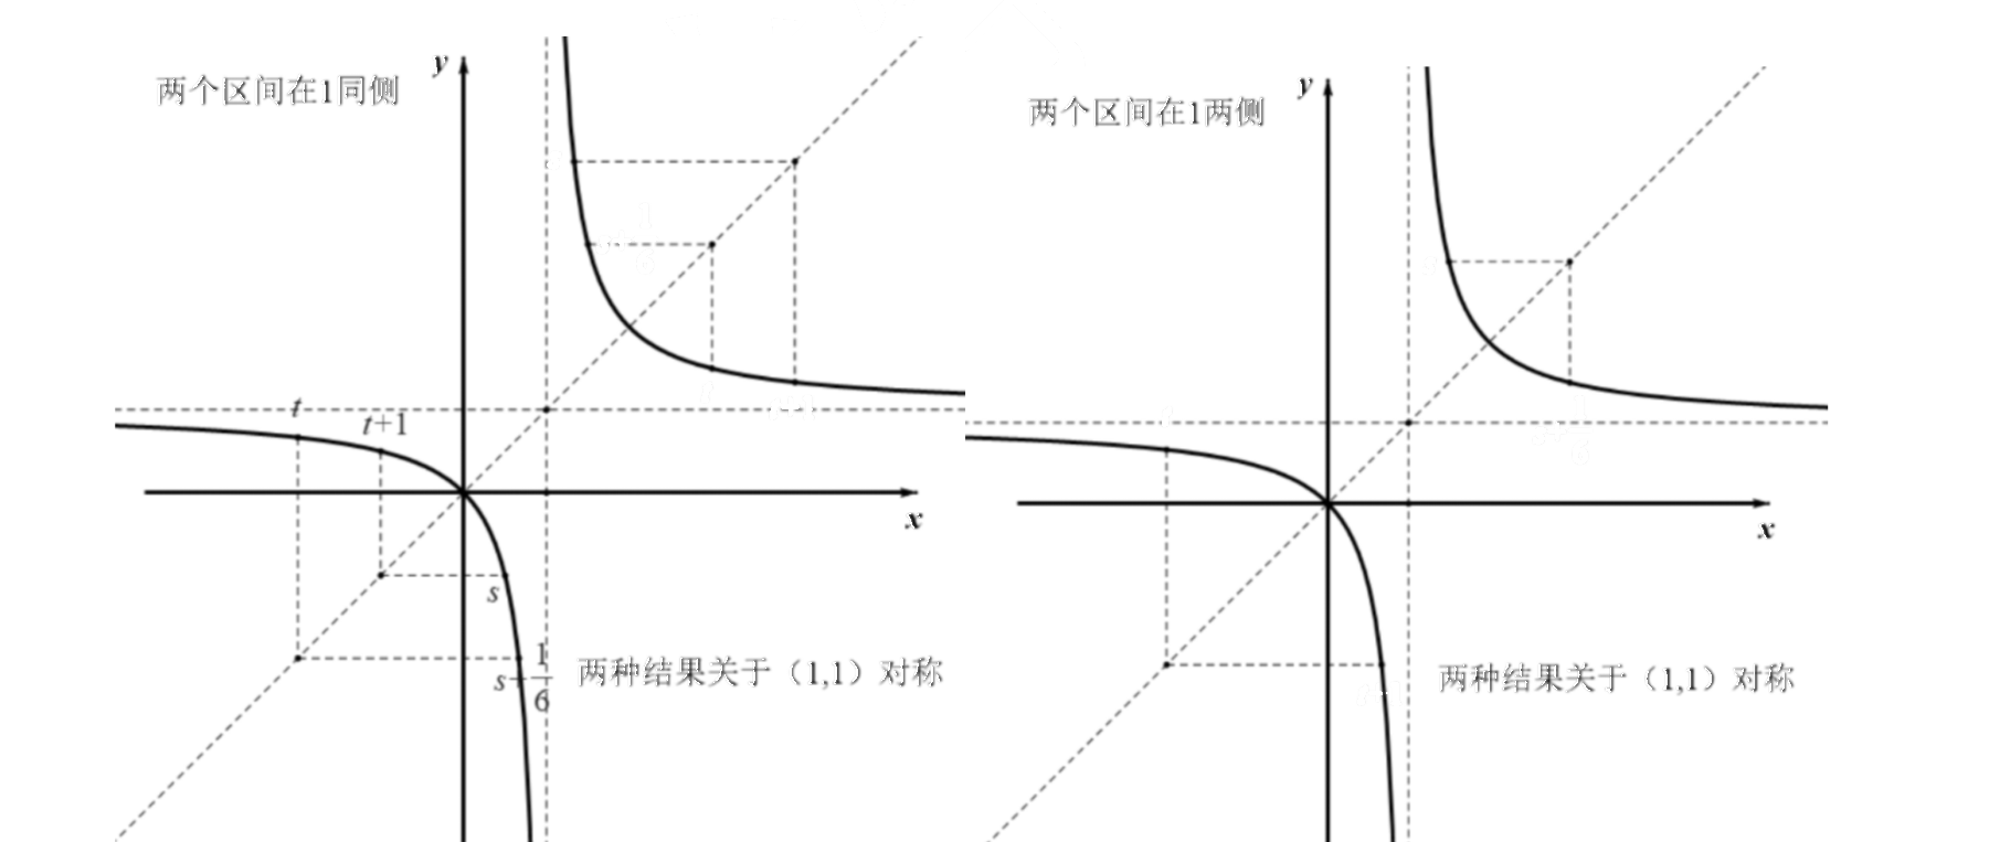
\includegraphics[width=0.92\textwidth]{figures/gao115_q10.png}
\end{center}
\solend
\fi

\end{enumerate}

\bigsec{二、选择题}

\begin{enumerate}
\setcounter{enumi}{10}

\item “对任意有理数 $x$ 都有 $x^2\neq2$”的否定形式是\mbox{（\quad）}% 原卷把答案“$B$”印在题干括号内、无【解析】

\keepwithprev
A. 存在有理数 $x$ 使得 $x^2\neq2$\qquad\qquad B. 存在有理数 $x$ 使得 $x^2=2$

C. 存在无理数 $x$ 使得 $x^2\neq2$\qquad\qquad D. 存在无理数 $x$ 使得 $x^2=2$

\ifanswer
\ans{$B$}
\fi

\item 已知 $a$、$b$ 都是实数，那么“$a^3>b^3$”是“$a^2>b^2$”的\mbox{（\quad）}

\keepwithprev
A. 充分不必要条件\qquad\qquad B. 必要不充分条件

C. 充要条件\qquad\qquad\qquad D. 既不充分也不必要条件

\ifanswer
\solbegin
\step{因为 $a^3>b^3$ 等价于 $a>b$，}
\step{由于 $a$、$b$ 正负不定，所以由 $a>b$ 不能得到 $a^2>b^2$，}
\step{由 $a^2>b^2$ 也不能得到 $a>b$，}
\step{因此“$a^3>b^3$”是“$a^2>b^2$”的既不充分也不必要条件. 故选 $D$.}
\solend
\fi

\item 定义集合运算 $A-B=\{x\mid x\in A$ 且 $x\notin B\}$，将 $A\triangle B=(A-B)\cup(B-A)$ 称为集合 $A$ 与集合 $B$ 的对称差.

命题一：$A\triangle B=B\triangle A$；

命题二：$A\triangle\varnothing=A$；

命题三：$A\cap(B\triangle C)=(A\cap B)\triangle(A\cap C)$；

命题四：$A\cup(B\triangle C)=(A\cup B)\triangle(A\cup C)$；

其中正确命题的个数是\mbox{（\quad）}

\keepwithprev
A. $1$\qquad\qquad B. $2$\qquad\qquad C. $3$\qquad\qquad D. $4$

\ifanswer
\solbegin
\step{对于①，$B\triangle A=(B-A)\cup(A-B)=(A-B)\cup(B-A)=A\triangle B$，①对；}
\step{对于②，$A-B=\{x\mid x\in A$ 且 $x\notin B\}=\{x\mid x\in A$ 且 $x\notin(A\cap B)\}$}
\step{$=A-(A\cap B)$，则 $A\triangle\varnothing=(A-\varnothing)\cup(\varnothing-A)=A\cup\varnothing=A$，②对；}
\step{对于③，$A\cap(B\triangle C)=A\cap(B\cup C-B\cap C)=A\cap(B\cup C)-A\cap(B\cap C)$}
\step{$=(A\cap B)\cup(A\cap C)-(A\cap B)\cap(A\cap C)=(A\cap B)\triangle(A\cap C)$，③对；}
\step{对于④，如图所示：}
\begin{center}
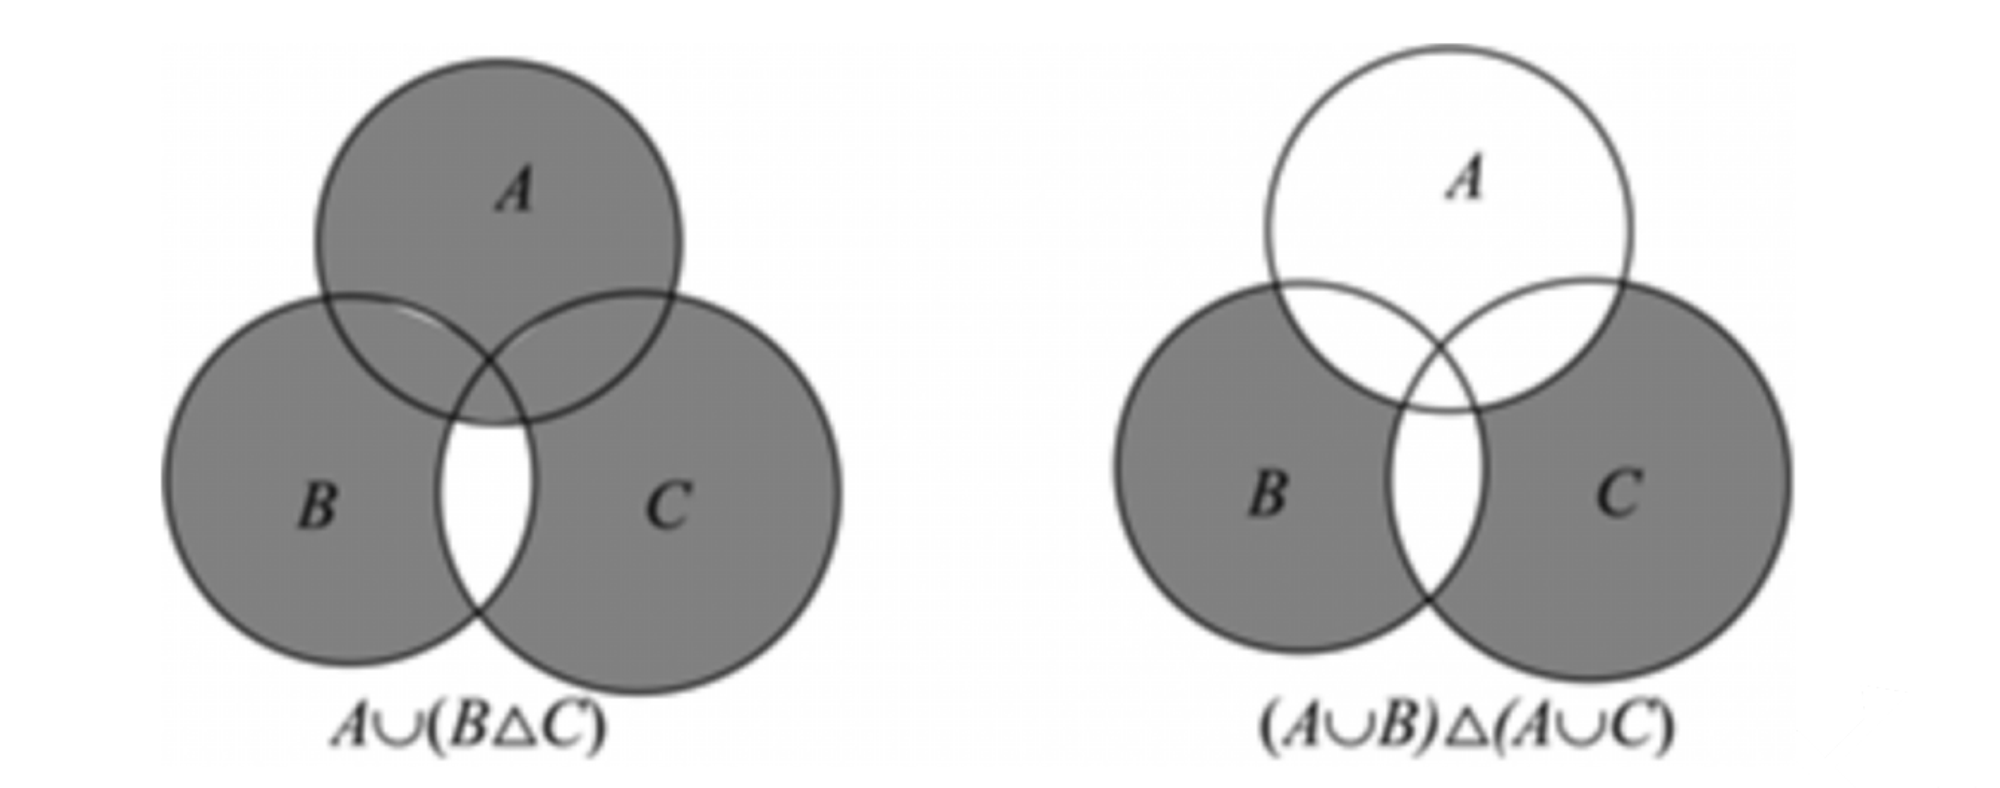
\includegraphics[width=0.85\textwidth]{figures/gao115_q13.png}
\end{center}
\step{所以 $A\cup(B\triangle C)\neq(A\cup B)\triangle(A\cup C)$，④错.}
\step{故选 $C$.}
\solend
\fi

\item 设 $a$、$b$、$c$、$p$ 为实数，若同时满足不等式 $ax^2+bx+c>0$、$bx^2+cx+a>0$ 与 $cx^2+ax+b>0$ 的全体实数 $x$ 所组成的集合等于 $(p,+\infty)$，则关于结论：① $a$、$b$、$c$ 至少有一个为 $0$；② $p=0$. 下列判断中正确的是\mbox{（\quad）}

\keepwithprev
A. ①和②都正确\qquad B. ①和②都错误\qquad C. ①正确，②错误\qquad D. ①错误，②正确

\ifanswer
\solbegin
\step{若同时满足不等式 $ax^2+bx+c>0$、$bx^2+cx+a>0$ 与 $cx^2+ax+b>0$ 的}
\step{全体实数 $x$ 所组成的集合等于 $(p,+\infty)$，必有 $a$,$b$,$c\geqslant0$，}
\step{不妨假设 $a$、$b$、$c$ 没有一个为 $0$，}
\step{则三个不等式均为开口向上的二次函数大于 $0$ 的部分，}
\step{解集的交集应为 $(-\infty,m)\cup(n,+\infty)$ 的形式，矛盾，}
\step{所以 $a$、$b$、$c$ 至少有一个为 $0$，故①正确：}
\step{不妨设 $a=0$，则 $b$,$c\geqslant0$，则不等式组化为 $\begin{cases}bx+c>0\\bx^2+cx>0,\\cx^2+b>0\end{cases}$}
\step{所以 $\begin{cases}x>-\dfrac cb\\x<-\dfrac cb\text{或}x>0\\x\in\R\end{cases}$，取交集得 $(0,+\infty)$，故 $p=0$，故②正确：}
\step{故选 $A$.}
\solend
\fi

\end{enumerate}

\bigsec{三、解答题}

\begin{enumerate}
\setcounter{enumi}{14}

\item 已知 $a>0$，$b>0$，

（1）试比较 $\dfrac{a^2-b^2}{a^2+b^2}$ 与 $\dfrac{a-b}{a+b}$ 的大小；

（2）若 $a+b>4$，求证：$\dfrac a{b+2}$ 和 $\dfrac b{a+2}$ 中至少有一个大于 $\dfrac12$.

\ifanswer
\solbegin
\step{（1）已知 $a>0$，$b>0$，$\dfrac{a^2-b^2}{a^2+b^2}-\dfrac{a-b}{a+b}=\dfrac{2ab(a-b)}{(a^2+b^2)(a+b)}$，}
\step{当 $a>b$ 时，$a-b>0$，所以 $\dfrac{a^2-b^2}{a^2+b^2}-\dfrac{a-b}{a+b}>0$，所以 $\dfrac{a^2-b^2}{a^2+b^2}>\dfrac{a-b}{a+b}$；}
\step{当 $a=b$ 时，$a-b=0$，所以 $\dfrac{a^2-b^2}{a^2+b^2}-\dfrac{a-b}{a+b}=0$，所以 $\dfrac{a^2-b^2}{a^2+b^2}=\dfrac{a-b}{a+b}$；}
\step{当 $a<b$ 时，$a-b<0$，所以 $\dfrac{a^2-b^2}{a^2+b^2}-\dfrac{a-b}{a+b}<0$，所以 $\dfrac{a^2-b^2}{a^2+b^2}<\dfrac{a-b}{a+b}$；}
\step{（2）假设 $\dfrac a{b+2}$ 和 $\dfrac b{a+2}$ 中都不大于 $\dfrac12$，即 $\dfrac b{a+2}\leqslant\dfrac12$，$\dfrac a{b+2}\leqslant\dfrac12$，}
\step{因为 $a>0$，$b>0$，所以 $a+2>0$，$b+2>0$，}
\step{所以 $2b\leqslant a+2$，$2a\leqslant b+2$，}
\step{两式相加得 $2a+2b\leqslant a+2+b+2=a+b+4$，即 $a+b\leqslant4$，}
\step{与已知 $a+b>4$ 矛盾，所以假设错误，}
\step{故 $\dfrac a{b+2}$ 和 $\dfrac b{a+2}$ 中至少有一个大于 $\dfrac12$.}
\solend
\fi

\item 某企业原有 $200$ 名科技人员，年人均工资 $a$ 万元($a>0$). 现加大对某芯片研发力度，该企业把原有 $200$ 名科技人员调整成技术人员和研发人员，其中技术人员 $x$ 名($x\in\N$ 且 $40\leqslant x\leqslant80$). 调整后，研发人员的年人均工资比调整前增加了 $(2x)\%$，技术人员的年人均工资为 $a\left(m-\dfrac x{10}\right)$万元.

（1）若要使调整后研发人员的年总工资不低于调整前 $200$ 名科技人员年总工资的 $1.5$ 倍，求调整后的技术人员最少有多少人？

（2）为了激励研发人员的工作热情和保持技术人员的工作积极性，企业决定在工资方面要同时满足以下两个条件：

①研发人员的年总工资始终不低于技术人员的年总工资；

②技术人员的年人均工资始终不低于调整前 $200$ 名科技人员的年人均工资.

请问是否存在这样的实数 $m$？若存在，求出 $m$ 的范围；若不存在，说明理由.

\ifanswer
\solbegin
\step{（1）由题意得调整后研发人员的年人均工资为 $[1+(2x)\%]a$ 万元，}
\step{那么 $(200-x)[1+(2x)\%]a\geqslant1.5\times200a$ ($a>0$)，}
\step{化简得 $x^2-150x+5000\leqslant0$，解得 $50\leqslant x\leqslant100$，}
\step{由于 $x\in\N$ 且 $40\leqslant x\leqslant80$，因此 $50\leqslant x\leqslant80$，}
\step{因此调整后的技术人员的人数最少为 $50$ 人；}
\step{（2）假设存在实数 $m$，使得技术人员在已知范围内调整后，满足以上两个条件，}
\step{由条件①得 $(200-x)[1+(2x)\%]a\geqslant x\left(m-\dfrac x{10}\right)a$，}
\step{整理得 $m\leqslant\dfrac{200}{x}+\dfrac{2x}{25}+3$；}
\step{因为 $\dfrac{200}{x}+\dfrac{2x}{25}+3\geqslant2\sqrt{\dfrac{200}{x}\cdot\dfrac{2x}{25}}+3=11$，}
\step{当且仅当 $\dfrac{200}{x}=\dfrac{2x}{25}$，即 $x=50$ 时取等号，因此 $m\leqslant11$，}
\step{由条件②得 $a\left(m-\dfrac x{10}\right)\geqslant a$，所以 $m\geqslant\dfrac x{10}+1$；}
\step{又由于 $40\leqslant x\leqslant80$，因此 $m\geqslant9$.}
\step{因此 $m\in[9,11]$.}
\solend
\fi

\item 已知 $a\in\R$，记 $f(x)=ax^2-(a+2)x+2$.

（1）若 $f(x)<3-2x$ 对于一切 $x\in\R$ 恒成立，求实数 $a$ 的取值范围；

（2）求关于 $x$ 不等式 $f(x)\geqslant0$ 的解集；

（3）若存在 $m\in\R$ 使关于 $x$ 的方程 $ax^2-(a+2)\lvert x\rvert+2=\lvert m+2\rvert+\lvert m-1\rvert$ 有四个不同的实根，求实数 $a$ 的取值范围.

\ifanswer
\solbegin
\step{（1）由 $f(x)<3-2x$ 对于一切 $x\in\R$ 恒成立，}
\step{得 $ax^2-ax-1<0$ 对于一切 $x\in\R$ 恒成立，}
\step{当 $a=0$ 时，原式可化为 $-1<0$，恒成立，符合条件；}
\step{当 $a\neq0$ 时，需满足 $\begin{cases}a<0\\\Delta=a^2+4a<0\end{cases}$，解得 $-4<a<0$；}
\step{综上，实数 $a$ 的取值范围是 $(-4,0]$；}
\step{（2）$f(x)\geqslant0$，即 $(ax-2)(x-1)\geqslant0$，}
\step{当 $a=0$ 时，原式化为 $-2x+2\geqslant0$，解集为 $\{x\mid x\leqslant1\}$；}
\step{当 $a>0$ 时，若 $a=2$，原式化为 $2(x-1)^2\geqslant0$，解集为 $\R$；}
\step{若 $0<a<2$，$\dfrac2a>1$，解集为 $\{x\mid x\leqslant1$ 或 $x\geqslant\dfrac2a\}$；}
\step{若 $a>2$，$\dfrac2a<1$，解集为 $\{x\mid x\leqslant\dfrac2a$ 或 $x\geqslant1\}$；}
\step{当 $a<0$ 时，$\dfrac2a<1$，解集为 $\left\{x\,\middle\vert\,\dfrac2a\leqslant x\leqslant1\right\}$；}
\step{综上，当 $a<0$ 时，不等式解集为 $\left\{x\,\middle\vert\,\dfrac2a\leqslant x\leqslant1\right\}$；}
\step{当 $a=0$ 时，不等式解集为 $\{x\mid x\leqslant1\}$；}
\step{当 $0<a<2$ 时，不等式解集为 $\{x\mid x\leqslant1$ 或 $x\geqslant\dfrac2a\}$；}
\step{当 $a=2$ 时，不等式解集为 $\R$；}
\step{当 $a>2$ 时，不等式解集为 $\{x\mid x\leqslant\dfrac2a$ 或 $x\geqslant1\}$；}
\step{（3）由绝对值三角不等式得 $\lvert m+2\rvert+\lvert m-1\rvert\geqslant\lvert(m+2)-(m-1)\rvert=3$，}
\step{即右侧取值范围为 $[3,+\infty)$，}
\step{令 $t=\lvert x\rvert\geqslant0$，原方程转化为 $at^2-(a+2)t+2=k$，$k\in[3,+\infty)$，}
\step{若原方程有四个不同实根，}
\step{需存在 $k\geqslant3$，使得方程 $at^2-(a+2)t+2-k=0$ 有两个不同正实根，}
\step{当 $a\geqslant0$ 时，方程的两根之积为 $\dfrac{2-k}{a}$，}
\step{因为 $k\geqslant3$，所以 $2-k\leqslant-1<0$，两根一正一负，}
\step{最多只有一个正根，对应最多两个 $x$ 根，不符合要求；}
\step{当 $a<0$ 时，两根之积为正，}
\step{要两个根都为正，需要两根之和 $\dfrac{a+2}{a}>0$，解得 $a<-2$，}
\step{再要求存在 $k\geqslant3$ 使得判别式大于 $0$，}
\step{即 $\triangle=(a+2)^2-4a(2-k)>0$ 在 $k\in[3,+\infty)$ 上有解，}
\step{即 $(a-2)^2+4ak>0$ 在 $k\in[3,+\infty)$ 上有解，}
\step{由 $a<0$，得 $(a-2)^2+12a>0$，}
\step{即 $a^2+8a+4>0$，结合 $a<-2$ 解得 $a<-4-2\sqrt3$，}
\step{故实数 $a$ 的取值范围是 $(-\infty,-4-2\sqrt3)$.}
\solend
\fi

\item 设 $A=\{x_1,x_2,\cdots,x_n\}(n\geqslant2,n\in\N)$，且 $x_1,x_2,\cdots,x_n$ 均为正整数，若对于 $A$ 中任意两个元素 $a,b$，当 $a>b$ 时，都有 $\dfrac{b^2}{a-b}\in A$，则称 $A$ 为“$n$ 元好集”.

（1）判断 $\{2,4,6\}$ 是否为“三元好集”，并说明理由；

（2）若集合 $M$ 为“二元好集”，且 $M$ 中所有元素之积小于 $2026$，求所有满足条件的集合 $M$ 的个数；

（3）设 $k\geqslant3,k\in\N$，是否存在“$k$ 元好集”，若存在，求出所有满足条件的“$k$ 元好集”，若不存在，请说明理由.

\ifanswer
\solbegin
\step{（1）取 $a=6,b=2$，则 $\dfrac{b^2}{a-b}=\dfrac44=1\notin\{2,4,6\}$，所以该集合不是三元好集.}
\step{（2）设 $M=\{b,a\}$，其中 $a>b$ 且均为正整数，则 $\dfrac{b^2}{a-b}$ 等于 $a$ 或 $b$.}
\step{若 $\dfrac{b^2}{a-b}=a$，则 $a^2-ab-b^2=0$，从而 $\dfrac ab=\dfrac{1+\sqrt5}{2}$，与 $\dfrac ab$ 为有理数矛盾.}
\step{若 $\dfrac{b^2}{a-b}=b$，则 $a=2b$；}
\step{反之，任意正整数 $b$ 对应的 $\{b,2b\}$ 均为二元好集.}
\step{由元素之积小于 $2026$，得 $2b^2<2026\Leftrightarrow b^2<1013$.}
\step{因为 $31^2=961<1013<1024=32^2$，所以 $b=1,2,\cdots,31$，}
\step{对应 $31$ 个不同的集合.}
\step{（3）假设存在 $k\geqslant3$ 的 $k$ 元好集 $A$，将其元素从小到大排列，}
\step{记最小元素为 $u$，次小元素为 $v$，最大元素为 $w$，则 $0<u<v<w$.}
\step{由 $\dfrac{u^2}{w-u}\in A$，该数不小于 $u$，得 $\dfrac{u^2}{w-u}\geqslant u\Rightarrow w\leqslant2u$.}
\step{又由 $\dfrac{u^2}{v-u}$,$\dfrac{v^2}{w-v}\in A$，这两个数均不超过 $w$，}
\step{得 $\dfrac{u^2}{v-u}\leqslant w$,$\dfrac{v^2}{w-v}\leqslant w$，}
\step{分母均为正，分别去分母后相加，}
\step{得 $u^2+v^2\leqslant w(v-u)+w(w-v)=w(w-u)\leqslant2u^2$，}
\step{于是 $v^2\leqslant u^2$，与 $v>u>0$ 矛盾，所以不存在 $k\geqslant3$ 的 $k$ 元好集.}
\solend
\fi

\end{enumerate}

\end{document}
"
% 紧凑版：xelatex "\def\iscompact{1}% 高一115_复旦附中_10月阶段练习.tex
%   —— 高一上数学“2026-2027 年复旦附中高一上 10 月阶段练习”（试卷版/答案版）
% 试卷版：xelatex 高一115_复旦附中_10月阶段练习.tex
% 答案版：xelatex "\def\isanswer{1}\input{高一115_复旦附中_10月阶段练习.tex}"
% 紧凑版：xelatex "\def\iscompact{1}\input{高一115_复旦附中_10月阶段练习.tex}"
%
% 原始材料：微信公众号“魔都数学加油站”文章，作者破晓，2026-11-06 17:58 发布；
% 连载“27学年高一115”，原文标题“27学年高一115——2026-2027年上海市复旦附中高一上10月阶段练习”；
% 原文链接：https://mp.weixin.qq.com/s/krocP0fMQQ4VM1SQEcLI2Q。
% 正文为 12 张 PNG 页（第 4、6、12 页 2560×3620，其余 4762×6735），
% 题目下印有【解析】或【答案】，为讲评版。
% 题目、解析均据原图转录；卷面红色水印及公众号页脚未录入。
%
% 卷首标题：原卷印作“2026-2027 年复旦附中高一上 10 月阶段练习”（公众号标题中的“上海市”
% 卷面标题行没有，本稿照卷面），年份区间按全稿惯例排 en dash；原卷未印副标题，本稿按题目内容
% 标为“集合与常用逻辑用语、不等式”。
%
% 与原卷的排版差异：
%   ① 原文从第 3 题起，填空题编号为 3—10、选择题为 11—14、解答题为 15—18，共 16 题，
%      本稿保留原题号（与多数卷的 3—21 不同）；
%   ② 原卷每题下直接印【解析】／【答案】，本稿按全稿惯例置于答案版；第 11 题把答案“$B$”
%      印在题干括号内且无【解析】，另提 \ans{}；其余选择题答案在解析末句“故选 …”，括号内留空；
%   ③ 原卷未印副标题，本稿按“知识模块”口径补出；
%   ④ 原卷填空横线按全稿惯例排为 \blankline[4.4em]；选择题括号排 \mbox{（\quad）}、
%      选项段前按惯例加 \keepwithprev；解答题不留作答区（原卷为讲评版，与 109—114 同）；
%   ⑤ 原卷数集排斜体 $R$／$Q$／$N$，按全稿惯例改 \R、\Q、\N。
%
% 判别式与对称差字形：原卷 $\triangle$（等边、扁）与 $\Delta$（等腰、高）两种混用，逐处照录——
%   第 7 题与第 17 题 (3) 的判别式、第 13 题的对称差 $A\triangle B$ 用 \triangle，
%   第 17 题 (1) cases 的判别式用 \Delta。
%
% 子集符号：第 4 题解析的 $(-1,3)\subset(-m,m)$ 印单线（真子集、无下划线），按 18／96
%   成例照录 \subset；第 5 题解析的 $B\subseteq A$ 印有下划线，照录 \subseteq。
%   第 3 题的补集照原卷上划线排 \overline{N}。
%
% 原卷存疑照录：第 9 题解析末行“故可能成立的是①②③”与四种情形的编号一致，照录；
%   第 10 题解析两幅函数图上另有蓝色／红色手写标注（$t$、$t+1$、$s$、$\frac16$ 等），
%   系批改笔迹，随裁图保留、不另作正文录入；第 14 题解析的 cases 三行照原卷排；
%   第 18 题 (2) 解析“所以该集合不是三元好集”前的取例 $a=6,b=2$ 照录。
%
% 行数核对：逐题数 \step/\stepm 条数，合计 133 条（Q3：3；Q4：3；Q5：4；Q6：5；Q7：4；
% Q8：4；Q9：11；Q10：7；Q11：0；Q12：4；Q13：8；Q14：9；Q15：10；Q16：13；
% Q17：32；Q18：16），与原卷印刷行逐题相等（cases 块作一个印刷行计）。第 11 题括号内印
% 答案且无解析，提 \ans{}，不计入 \step 账；第 10、13 题解析内的插图不计入 \step 账。
%
\documentclass[a4paper,11pt]{article}
\usepackage{common}

\begin{document}

\examtitlest[3]{2026--2027 年复旦附中高一上 10 月阶段练习}{集合与常用逻辑用语、不等式}

\bigsec{一、填空题}

\begin{enumerate}
\setcounter{enumi}{2}

\item 已知集合 $M=\{x\mid 4x^2-4x-15>0\}$，$N=\left\{x\,\middle\vert\,\dfrac{x+1}{x-6}>0\right\}$，则 $M\cap\overline{N}=$\blankline[4.4em].

\ifanswer
\solbegin
\step{集合 $M=\{x\mid 4x^2-4x-15>0\}=\{x\mid x>\dfrac52$ 或 $x<-\dfrac32\}$，}
\step{$N=\left\{x\,\middle\vert\,\dfrac{x+1}{x-6}>0\right\}=\{x\mid x>6$ 或 $x<-1\}$，得 $\overline{N}=\{x\mid-1\leqslant x\leqslant6\}$，}
\step{故 $M\cap\overline{N}=\left\{x\,\middle\vert\,\dfrac52<x\leqslant6\right\}$.}
\solend
\fi

\item 已知 $m>0$，不等式 $\lvert x\rvert<m$ 成立的一个充分不必要条件是 $-1<x<3$，则 $m$ 的取值范围是\blankline[4.4em].

\ifanswer
\solbegin
\step{不等式 $-m<x<m$ 成立的一个充分不必要条件是 $-1<x<3$，}
\step{由题意得 $(-1,3)\subset(-m,m)$，则 $m\geqslant3$，此时 $-m\leqslant-3<-1$，}% 原卷印单线 \subset，照录
\step{所以 $m$ 的取值范围是 $\{m\mid m\geqslant3\}$.}
\solend
\fi

\item 已知集合 $A=\{1,2\}$，集合 $B=\{x\mid ax=6\}$，若 $A\cup B=A$，则 $a$ 的所有取值构成的集合为\blankline[4.4em].

\ifanswer
\solbegin
\step{因为 $A\cup B=A$，所以 $B\subseteq A$，}
\step{当 $a=0$ 时，$B=\varnothing$，满足 $B\subseteq A$；}
\step{当 $a\neq0$ 时，$B=\left\{\dfrac6a\right\}$，则 $\dfrac6a=1$ 或 $\dfrac6a=2$，解得 $a=6$ 或 $a=3$，}
\step{综上所述，$a$ 的所有取值构成的集合为 $\{0,3,6\}$.}
\solend
\fi

\item 若关于 $x$ 的不等式 $ax^2+bx+c>0$ 的解集为 $(-3,2)$，则不等式 $ax^2+(a+b)x+c-2a>0$ 的解集为\blankline[4.4em].

\ifanswer
\solbegin
\step{由 $ax^2+bx+c>0$ 的解集为 $(-3,2)$ 得 $a<0$，}
\step{且 $ax^2+bx+c=0$ 时 $x_1=-3$，$x_2=2$，}
\step{得 $-3+2=-\dfrac ba$，即 $b=a$，$-3\times2=\dfrac ca$，即 $c=-6a$，}
\step{代入 $ax^2+(a+b)x+c-2a>0$ 得 $ax^2+2ax-8a>0$ 化简得 $x^2+2x-8<0$，}
\step{解得 $-4<x<2$，故解集为 $(-4,2)$.}
\solend
\fi

\item 已知关于 $x$ 的方程 $x^2-2x+m=0$ 的两个实数根分别为 $x_1$，$x_2$. 若 $x_1^2x_2^2+x_1^2+x_2^2=7$，则实数 $m$ 的值为\blankline[4.4em].

\ifanswer
\solbegin
\step{由韦达定理得 $x_1+x_2=2$，$x_1x_2=m$，}
\step{$x_1^2x_2^2+x_1^2+x_2^2=(x_1x_2)^2+(x_1+x_2)^2-2x_1x_2=m^2+4-2m$，}
\step{由 $m^2+4-2m=7$，得 $m^2-2m-3=0$，解得 $m=3$ 或 $m=-1$，}
\step{方程有两个实数根，故 $\triangle=4-4m\geqslant0$，即 $m\leqslant1$，所以 $m=-1$.}
\solend
\fi

\item 已知 $x>1$，若 $x^2-xy+y=0$，则 $x+y$ 的最小值是\blankline[4.4em].

\ifanswer
\solbegin
\step{由于 $x^2-xy+y=0$，则 $y=\dfrac{x^2}{x-1}>0$，}
\step{则 $x+y=x+\dfrac{x^2}{x-1}=\dfrac{2x^2-x}{x-1}=\dfrac{2(x-1)^2+3(x-1)+1}{x-1}$}
\step{$=2(x-1)+\dfrac1{x-1}+3\geqslant2\sqrt{2(x-1)\cdot\dfrac1{x-1}}+3=2\sqrt2+3$，}
\step{当且仅当 $x=1+\dfrac{\sqrt2}{2}$ 时取等号，故最小值是 $2\sqrt2+3$.}
\solend
\fi

\item 若集合 $A=B_1\cup B_2\cup\cdots\cup B_n$，其中 $B_1$、$B_2$、$\cdots$、$B_n$ 为非空集合，$B_i\cap B_j=\varnothing$，$1\leqslant i<j\leqslant n$，则称集合 $\{B_1,B_2,\cdots,B_n\}$ 为集合 $A$ 的一个 $n$ 划分. 例如：集合 $\{\{1,2\},\{3\}\}$，$\{\{1,3\},\{2\}\}$，$\{\{2,3\},\{1\}\}$ 均为集合 $\{1,2,3\}$ 的一个 $2$ 划分. 设 $\{B_1,B_2\}$ 为有理数集 $\Q$ 的一个 $2$ 划分，且满足对任意 $x\in B_1$，任意 $y\in B_2$，都有 $x<y$. 则对于 $B_1$、$B_2$ 有：

① $B_1$ 中的元素存在最大值，$B_2$ 中的元素不存在最小值；

② $B_1$ 中的元素不存在最大值，$B_2$ 中的元素存在最小值；

③ $B_1$ 中的元素不存在最大值，$B_2$ 中的元素不存在最小值；

④ $B_1$ 中的元素存在最大值，$B_2$ 中的元素存在最小值；

对于以上四种情况，可能成立的序号有\blankline[4.4em].

\ifanswer
\solbegin
\step{对于①，$B_1=\{x\in\Q\mid x\leqslant2\}$，$B_2=\{x\in\Q\mid x>2\}$，①可能成立；}
\step{对于②，$B_1=\{x\in\Q\mid x<2\}$，$B_2=\{x\in\Q\mid x\geqslant2\}$，②可能成立；}
\step{对于③，$B_1=\{x\in\Q\mid x<\pi\}$，$B_2=\{x\in\Q\mid x>\pi\}$，③可能成立；}
\step{对于④，假设④成立，}
\step{不妨设 $B_1$ 中的元素的最大值为 $s$，$B_2$ 中的元素的最小值为 $t$，}
\step{由题意得 $s<t$，所以 $s<\dfrac{s+t}{2}<t$，}
\step{因为 $s$ 为 $B_1$ 中的元素的最大值，所以 $\dfrac{s+t}{2}\notin B_1$，}
\step{因为 $t$ 为 $B_2$ 中的元素的最小值，所以 $\dfrac{s+t}{2}\notin B_2$，}
\step{又 $B_1\cup B_2=\Q$，所以 $\dfrac{s+t}{2}\notin\Q$，与 $\dfrac{s+t}{2}\in\Q$ 矛盾，}
\step{所以假设不成立，即④不可能成立.}
\step{故可能成立的是①②③.}
\solend
\fi

\item 已知集合 $A=\left[s,s+\dfrac16\right]\cup[t,t+1]$，其中 $1\notin A$ 且 $s+\dfrac16<t$，函数 $f(x)=\dfrac x{x-1}$，且对任意 $a\in A$，都有 $f(a)\in A$，则 $t$ 的值是\blankline[4.4em].

\ifanswer
\solbegin
\step{若 $\left[s,s+\dfrac16\right]$,$[t,t+1]$ 在 $f(x)=\dfrac x{x-1}$ 图像的同侧，}
\step{则点 $\left(t,s+\dfrac16\right)$,$(t+1,s)$ 在 $f(x)=\dfrac x{x-1}$ 的图像上，}
\step{所以 $\dfrac t{t-1}=\dfrac{t+1}{t}+\dfrac16$，解得 $t=-2$ 或 $t=3$，检验得 $t=3$；}
\step{若 $\left[s,s+\dfrac16\right]$,$[t,t+1]$ 在 $f(x)=\dfrac x{x-1}$ 图像的两侧，}
\step{则点 $(t,t+1)$ 在 $f(x)=\dfrac x{x-1}$ 的图像上，}
\step{所以 $t+1=\dfrac t{t-1}$，解得 $t=\dfrac{1\pm\sqrt5}{2}$，检验得 $t=\dfrac{1+\sqrt5}{2}$，}
\step{综上，$t=\dfrac{1+\sqrt5}{2}$ 或 $t=3$.}
\begin{center}
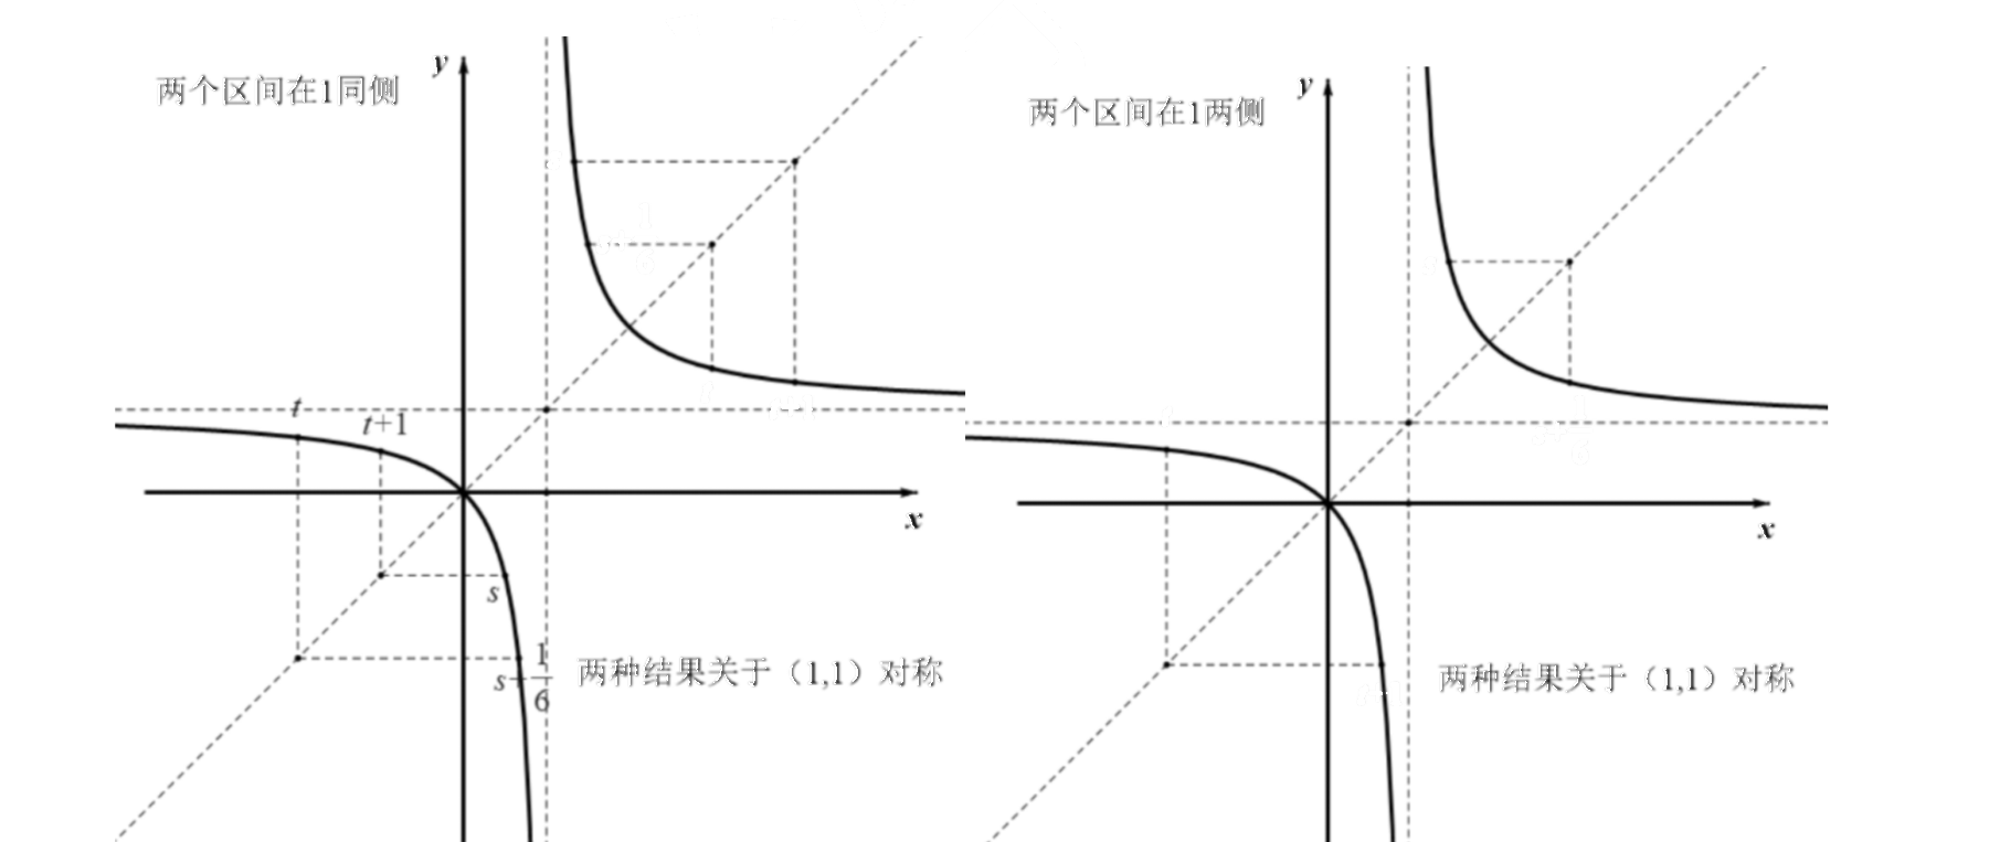
\includegraphics[width=0.92\textwidth]{figures/gao115_q10.png}
\end{center}
\solend
\fi

\end{enumerate}

\bigsec{二、选择题}

\begin{enumerate}
\setcounter{enumi}{10}

\item “对任意有理数 $x$ 都有 $x^2\neq2$”的否定形式是\mbox{（\quad）}% 原卷把答案“$B$”印在题干括号内、无【解析】

\keepwithprev
A. 存在有理数 $x$ 使得 $x^2\neq2$\qquad\qquad B. 存在有理数 $x$ 使得 $x^2=2$

C. 存在无理数 $x$ 使得 $x^2\neq2$\qquad\qquad D. 存在无理数 $x$ 使得 $x^2=2$

\ifanswer
\ans{$B$}
\fi

\item 已知 $a$、$b$ 都是实数，那么“$a^3>b^3$”是“$a^2>b^2$”的\mbox{（\quad）}

\keepwithprev
A. 充分不必要条件\qquad\qquad B. 必要不充分条件

C. 充要条件\qquad\qquad\qquad D. 既不充分也不必要条件

\ifanswer
\solbegin
\step{因为 $a^3>b^3$ 等价于 $a>b$，}
\step{由于 $a$、$b$ 正负不定，所以由 $a>b$ 不能得到 $a^2>b^2$，}
\step{由 $a^2>b^2$ 也不能得到 $a>b$，}
\step{因此“$a^3>b^3$”是“$a^2>b^2$”的既不充分也不必要条件. 故选 $D$.}
\solend
\fi

\item 定义集合运算 $A-B=\{x\mid x\in A$ 且 $x\notin B\}$，将 $A\triangle B=(A-B)\cup(B-A)$ 称为集合 $A$ 与集合 $B$ 的对称差.

命题一：$A\triangle B=B\triangle A$；

命题二：$A\triangle\varnothing=A$；

命题三：$A\cap(B\triangle C)=(A\cap B)\triangle(A\cap C)$；

命题四：$A\cup(B\triangle C)=(A\cup B)\triangle(A\cup C)$；

其中正确命题的个数是\mbox{（\quad）}

\keepwithprev
A. $1$\qquad\qquad B. $2$\qquad\qquad C. $3$\qquad\qquad D. $4$

\ifanswer
\solbegin
\step{对于①，$B\triangle A=(B-A)\cup(A-B)=(A-B)\cup(B-A)=A\triangle B$，①对；}
\step{对于②，$A-B=\{x\mid x\in A$ 且 $x\notin B\}=\{x\mid x\in A$ 且 $x\notin(A\cap B)\}$}
\step{$=A-(A\cap B)$，则 $A\triangle\varnothing=(A-\varnothing)\cup(\varnothing-A)=A\cup\varnothing=A$，②对；}
\step{对于③，$A\cap(B\triangle C)=A\cap(B\cup C-B\cap C)=A\cap(B\cup C)-A\cap(B\cap C)$}
\step{$=(A\cap B)\cup(A\cap C)-(A\cap B)\cap(A\cap C)=(A\cap B)\triangle(A\cap C)$，③对；}
\step{对于④，如图所示：}
\begin{center}
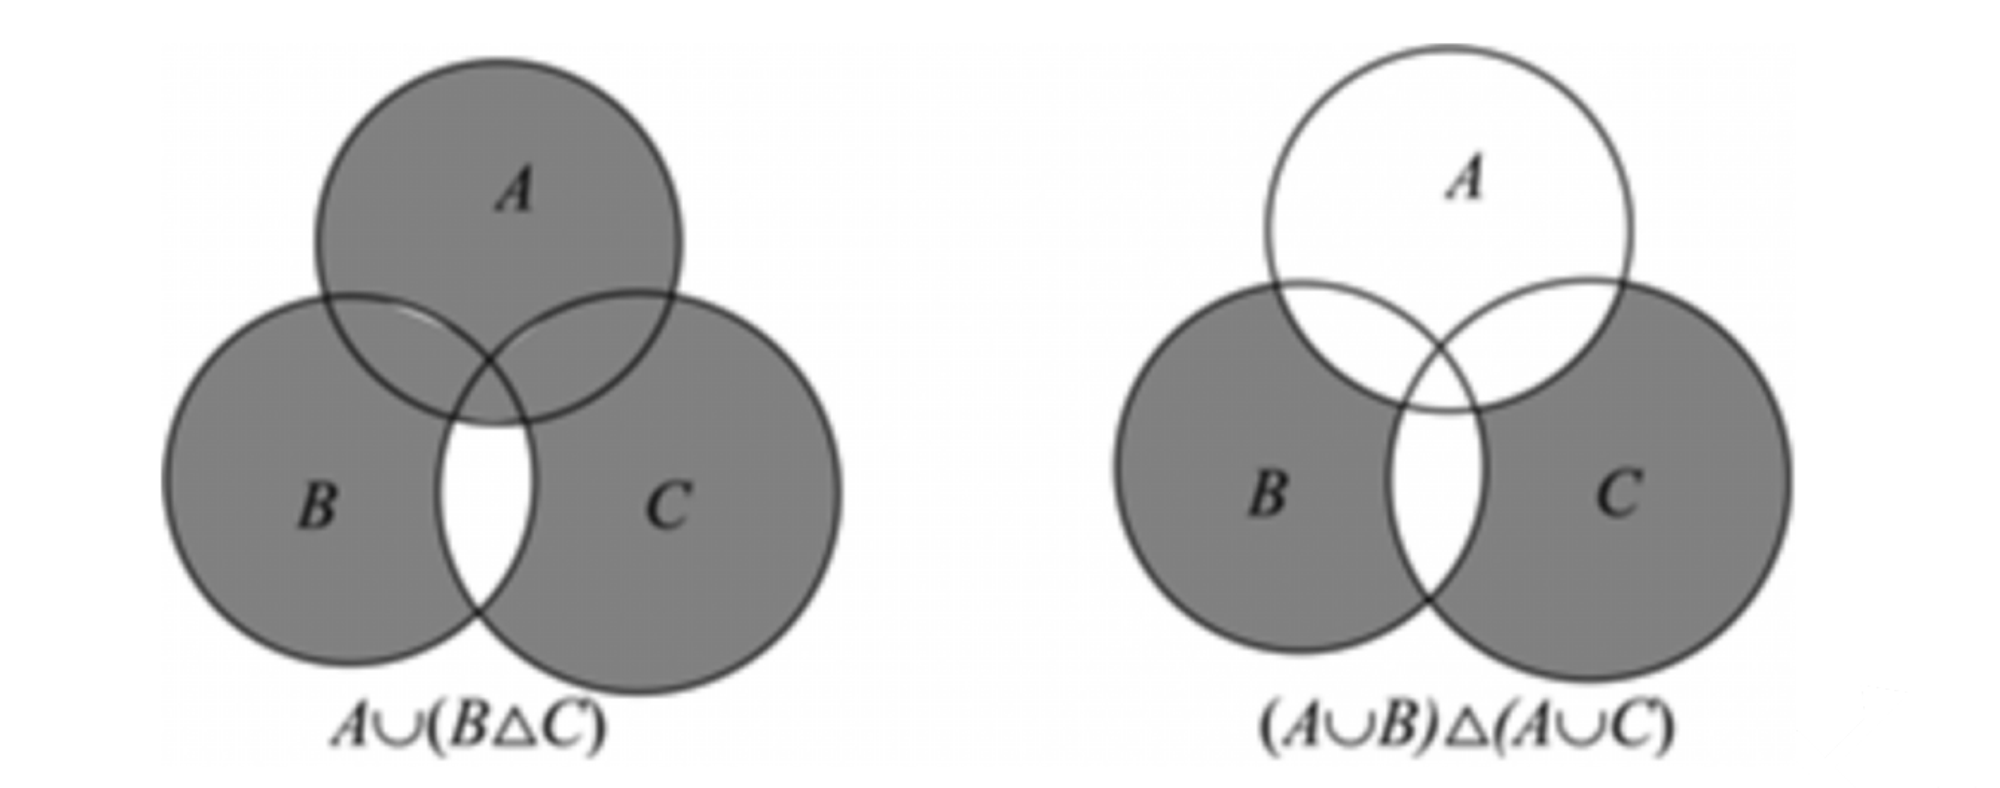
\includegraphics[width=0.85\textwidth]{figures/gao115_q13.png}
\end{center}
\step{所以 $A\cup(B\triangle C)\neq(A\cup B)\triangle(A\cup C)$，④错.}
\step{故选 $C$.}
\solend
\fi

\item 设 $a$、$b$、$c$、$p$ 为实数，若同时满足不等式 $ax^2+bx+c>0$、$bx^2+cx+a>0$ 与 $cx^2+ax+b>0$ 的全体实数 $x$ 所组成的集合等于 $(p,+\infty)$，则关于结论：① $a$、$b$、$c$ 至少有一个为 $0$；② $p=0$. 下列判断中正确的是\mbox{（\quad）}

\keepwithprev
A. ①和②都正确\qquad B. ①和②都错误\qquad C. ①正确，②错误\qquad D. ①错误，②正确

\ifanswer
\solbegin
\step{若同时满足不等式 $ax^2+bx+c>0$、$bx^2+cx+a>0$ 与 $cx^2+ax+b>0$ 的}
\step{全体实数 $x$ 所组成的集合等于 $(p,+\infty)$，必有 $a$,$b$,$c\geqslant0$，}
\step{不妨假设 $a$、$b$、$c$ 没有一个为 $0$，}
\step{则三个不等式均为开口向上的二次函数大于 $0$ 的部分，}
\step{解集的交集应为 $(-\infty,m)\cup(n,+\infty)$ 的形式，矛盾，}
\step{所以 $a$、$b$、$c$ 至少有一个为 $0$，故①正确：}
\step{不妨设 $a=0$，则 $b$,$c\geqslant0$，则不等式组化为 $\begin{cases}bx+c>0\\bx^2+cx>0,\\cx^2+b>0\end{cases}$}
\step{所以 $\begin{cases}x>-\dfrac cb\\x<-\dfrac cb\text{或}x>0\\x\in\R\end{cases}$，取交集得 $(0,+\infty)$，故 $p=0$，故②正确：}
\step{故选 $A$.}
\solend
\fi

\end{enumerate}

\bigsec{三、解答题}

\begin{enumerate}
\setcounter{enumi}{14}

\item 已知 $a>0$，$b>0$，

（1）试比较 $\dfrac{a^2-b^2}{a^2+b^2}$ 与 $\dfrac{a-b}{a+b}$ 的大小；

（2）若 $a+b>4$，求证：$\dfrac a{b+2}$ 和 $\dfrac b{a+2}$ 中至少有一个大于 $\dfrac12$.

\ifanswer
\solbegin
\step{（1）已知 $a>0$，$b>0$，$\dfrac{a^2-b^2}{a^2+b^2}-\dfrac{a-b}{a+b}=\dfrac{2ab(a-b)}{(a^2+b^2)(a+b)}$，}
\step{当 $a>b$ 时，$a-b>0$，所以 $\dfrac{a^2-b^2}{a^2+b^2}-\dfrac{a-b}{a+b}>0$，所以 $\dfrac{a^2-b^2}{a^2+b^2}>\dfrac{a-b}{a+b}$；}
\step{当 $a=b$ 时，$a-b=0$，所以 $\dfrac{a^2-b^2}{a^2+b^2}-\dfrac{a-b}{a+b}=0$，所以 $\dfrac{a^2-b^2}{a^2+b^2}=\dfrac{a-b}{a+b}$；}
\step{当 $a<b$ 时，$a-b<0$，所以 $\dfrac{a^2-b^2}{a^2+b^2}-\dfrac{a-b}{a+b}<0$，所以 $\dfrac{a^2-b^2}{a^2+b^2}<\dfrac{a-b}{a+b}$；}
\step{（2）假设 $\dfrac a{b+2}$ 和 $\dfrac b{a+2}$ 中都不大于 $\dfrac12$，即 $\dfrac b{a+2}\leqslant\dfrac12$，$\dfrac a{b+2}\leqslant\dfrac12$，}
\step{因为 $a>0$，$b>0$，所以 $a+2>0$，$b+2>0$，}
\step{所以 $2b\leqslant a+2$，$2a\leqslant b+2$，}
\step{两式相加得 $2a+2b\leqslant a+2+b+2=a+b+4$，即 $a+b\leqslant4$，}
\step{与已知 $a+b>4$ 矛盾，所以假设错误，}
\step{故 $\dfrac a{b+2}$ 和 $\dfrac b{a+2}$ 中至少有一个大于 $\dfrac12$.}
\solend
\fi

\item 某企业原有 $200$ 名科技人员，年人均工资 $a$ 万元($a>0$). 现加大对某芯片研发力度，该企业把原有 $200$ 名科技人员调整成技术人员和研发人员，其中技术人员 $x$ 名($x\in\N$ 且 $40\leqslant x\leqslant80$). 调整后，研发人员的年人均工资比调整前增加了 $(2x)\%$，技术人员的年人均工资为 $a\left(m-\dfrac x{10}\right)$万元.

（1）若要使调整后研发人员的年总工资不低于调整前 $200$ 名科技人员年总工资的 $1.5$ 倍，求调整后的技术人员最少有多少人？

（2）为了激励研发人员的工作热情和保持技术人员的工作积极性，企业决定在工资方面要同时满足以下两个条件：

①研发人员的年总工资始终不低于技术人员的年总工资；

②技术人员的年人均工资始终不低于调整前 $200$ 名科技人员的年人均工资.

请问是否存在这样的实数 $m$？若存在，求出 $m$ 的范围；若不存在，说明理由.

\ifanswer
\solbegin
\step{（1）由题意得调整后研发人员的年人均工资为 $[1+(2x)\%]a$ 万元，}
\step{那么 $(200-x)[1+(2x)\%]a\geqslant1.5\times200a$ ($a>0$)，}
\step{化简得 $x^2-150x+5000\leqslant0$，解得 $50\leqslant x\leqslant100$，}
\step{由于 $x\in\N$ 且 $40\leqslant x\leqslant80$，因此 $50\leqslant x\leqslant80$，}
\step{因此调整后的技术人员的人数最少为 $50$ 人；}
\step{（2）假设存在实数 $m$，使得技术人员在已知范围内调整后，满足以上两个条件，}
\step{由条件①得 $(200-x)[1+(2x)\%]a\geqslant x\left(m-\dfrac x{10}\right)a$，}
\step{整理得 $m\leqslant\dfrac{200}{x}+\dfrac{2x}{25}+3$；}
\step{因为 $\dfrac{200}{x}+\dfrac{2x}{25}+3\geqslant2\sqrt{\dfrac{200}{x}\cdot\dfrac{2x}{25}}+3=11$，}
\step{当且仅当 $\dfrac{200}{x}=\dfrac{2x}{25}$，即 $x=50$ 时取等号，因此 $m\leqslant11$，}
\step{由条件②得 $a\left(m-\dfrac x{10}\right)\geqslant a$，所以 $m\geqslant\dfrac x{10}+1$；}
\step{又由于 $40\leqslant x\leqslant80$，因此 $m\geqslant9$.}
\step{因此 $m\in[9,11]$.}
\solend
\fi

\item 已知 $a\in\R$，记 $f(x)=ax^2-(a+2)x+2$.

（1）若 $f(x)<3-2x$ 对于一切 $x\in\R$ 恒成立，求实数 $a$ 的取值范围；

（2）求关于 $x$ 不等式 $f(x)\geqslant0$ 的解集；

（3）若存在 $m\in\R$ 使关于 $x$ 的方程 $ax^2-(a+2)\lvert x\rvert+2=\lvert m+2\rvert+\lvert m-1\rvert$ 有四个不同的实根，求实数 $a$ 的取值范围.

\ifanswer
\solbegin
\step{（1）由 $f(x)<3-2x$ 对于一切 $x\in\R$ 恒成立，}
\step{得 $ax^2-ax-1<0$ 对于一切 $x\in\R$ 恒成立，}
\step{当 $a=0$ 时，原式可化为 $-1<0$，恒成立，符合条件；}
\step{当 $a\neq0$ 时，需满足 $\begin{cases}a<0\\\Delta=a^2+4a<0\end{cases}$，解得 $-4<a<0$；}
\step{综上，实数 $a$ 的取值范围是 $(-4,0]$；}
\step{（2）$f(x)\geqslant0$，即 $(ax-2)(x-1)\geqslant0$，}
\step{当 $a=0$ 时，原式化为 $-2x+2\geqslant0$，解集为 $\{x\mid x\leqslant1\}$；}
\step{当 $a>0$ 时，若 $a=2$，原式化为 $2(x-1)^2\geqslant0$，解集为 $\R$；}
\step{若 $0<a<2$，$\dfrac2a>1$，解集为 $\{x\mid x\leqslant1$ 或 $x\geqslant\dfrac2a\}$；}
\step{若 $a>2$，$\dfrac2a<1$，解集为 $\{x\mid x\leqslant\dfrac2a$ 或 $x\geqslant1\}$；}
\step{当 $a<0$ 时，$\dfrac2a<1$，解集为 $\left\{x\,\middle\vert\,\dfrac2a\leqslant x\leqslant1\right\}$；}
\step{综上，当 $a<0$ 时，不等式解集为 $\left\{x\,\middle\vert\,\dfrac2a\leqslant x\leqslant1\right\}$；}
\step{当 $a=0$ 时，不等式解集为 $\{x\mid x\leqslant1\}$；}
\step{当 $0<a<2$ 时，不等式解集为 $\{x\mid x\leqslant1$ 或 $x\geqslant\dfrac2a\}$；}
\step{当 $a=2$ 时，不等式解集为 $\R$；}
\step{当 $a>2$ 时，不等式解集为 $\{x\mid x\leqslant\dfrac2a$ 或 $x\geqslant1\}$；}
\step{（3）由绝对值三角不等式得 $\lvert m+2\rvert+\lvert m-1\rvert\geqslant\lvert(m+2)-(m-1)\rvert=3$，}
\step{即右侧取值范围为 $[3,+\infty)$，}
\step{令 $t=\lvert x\rvert\geqslant0$，原方程转化为 $at^2-(a+2)t+2=k$，$k\in[3,+\infty)$，}
\step{若原方程有四个不同实根，}
\step{需存在 $k\geqslant3$，使得方程 $at^2-(a+2)t+2-k=0$ 有两个不同正实根，}
\step{当 $a\geqslant0$ 时，方程的两根之积为 $\dfrac{2-k}{a}$，}
\step{因为 $k\geqslant3$，所以 $2-k\leqslant-1<0$，两根一正一负，}
\step{最多只有一个正根，对应最多两个 $x$ 根，不符合要求；}
\step{当 $a<0$ 时，两根之积为正，}
\step{要两个根都为正，需要两根之和 $\dfrac{a+2}{a}>0$，解得 $a<-2$，}
\step{再要求存在 $k\geqslant3$ 使得判别式大于 $0$，}
\step{即 $\triangle=(a+2)^2-4a(2-k)>0$ 在 $k\in[3,+\infty)$ 上有解，}
\step{即 $(a-2)^2+4ak>0$ 在 $k\in[3,+\infty)$ 上有解，}
\step{由 $a<0$，得 $(a-2)^2+12a>0$，}
\step{即 $a^2+8a+4>0$，结合 $a<-2$ 解得 $a<-4-2\sqrt3$，}
\step{故实数 $a$ 的取值范围是 $(-\infty,-4-2\sqrt3)$.}
\solend
\fi

\item 设 $A=\{x_1,x_2,\cdots,x_n\}(n\geqslant2,n\in\N)$，且 $x_1,x_2,\cdots,x_n$ 均为正整数，若对于 $A$ 中任意两个元素 $a,b$，当 $a>b$ 时，都有 $\dfrac{b^2}{a-b}\in A$，则称 $A$ 为“$n$ 元好集”.

（1）判断 $\{2,4,6\}$ 是否为“三元好集”，并说明理由；

（2）若集合 $M$ 为“二元好集”，且 $M$ 中所有元素之积小于 $2026$，求所有满足条件的集合 $M$ 的个数；

（3）设 $k\geqslant3,k\in\N$，是否存在“$k$ 元好集”，若存在，求出所有满足条件的“$k$ 元好集”，若不存在，请说明理由.

\ifanswer
\solbegin
\step{（1）取 $a=6,b=2$，则 $\dfrac{b^2}{a-b}=\dfrac44=1\notin\{2,4,6\}$，所以该集合不是三元好集.}
\step{（2）设 $M=\{b,a\}$，其中 $a>b$ 且均为正整数，则 $\dfrac{b^2}{a-b}$ 等于 $a$ 或 $b$.}
\step{若 $\dfrac{b^2}{a-b}=a$，则 $a^2-ab-b^2=0$，从而 $\dfrac ab=\dfrac{1+\sqrt5}{2}$，与 $\dfrac ab$ 为有理数矛盾.}
\step{若 $\dfrac{b^2}{a-b}=b$，则 $a=2b$；}
\step{反之，任意正整数 $b$ 对应的 $\{b,2b\}$ 均为二元好集.}
\step{由元素之积小于 $2026$，得 $2b^2<2026\Leftrightarrow b^2<1013$.}
\step{因为 $31^2=961<1013<1024=32^2$，所以 $b=1,2,\cdots,31$，}
\step{对应 $31$ 个不同的集合.}
\step{（3）假设存在 $k\geqslant3$ 的 $k$ 元好集 $A$，将其元素从小到大排列，}
\step{记最小元素为 $u$，次小元素为 $v$，最大元素为 $w$，则 $0<u<v<w$.}
\step{由 $\dfrac{u^2}{w-u}\in A$，该数不小于 $u$，得 $\dfrac{u^2}{w-u}\geqslant u\Rightarrow w\leqslant2u$.}
\step{又由 $\dfrac{u^2}{v-u}$,$\dfrac{v^2}{w-v}\in A$，这两个数均不超过 $w$，}
\step{得 $\dfrac{u^2}{v-u}\leqslant w$,$\dfrac{v^2}{w-v}\leqslant w$，}
\step{分母均为正，分别去分母后相加，}
\step{得 $u^2+v^2\leqslant w(v-u)+w(w-v)=w(w-u)\leqslant2u^2$，}
\step{于是 $v^2\leqslant u^2$，与 $v>u>0$ 矛盾，所以不存在 $k\geqslant3$ 的 $k$ 元好集.}
\solend
\fi

\end{enumerate}

\end{document}
"
%
% 原始材料：微信公众号“魔都数学加油站”文章，作者破晓，2026-11-06 17:58 发布；
% 连载“27学年高一115”，原文标题“27学年高一115——2026-2027年上海市复旦附中高一上10月阶段练习”；
% 原文链接：https://mp.weixin.qq.com/s/krocP0fMQQ4VM1SQEcLI2Q。
% 正文为 12 张 PNG 页（第 4、6、12 页 2560×3620，其余 4762×6735），
% 题目下印有【解析】或【答案】，为讲评版。
% 题目、解析均据原图转录；卷面红色水印及公众号页脚未录入。
%
% 卷首标题：原卷印作“2026-2027 年复旦附中高一上 10 月阶段练习”（公众号标题中的“上海市”
% 卷面标题行没有，本稿照卷面），年份区间按全稿惯例排 en dash；原卷未印副标题，本稿按题目内容
% 标为“集合与常用逻辑用语、不等式”。
%
% 与原卷的排版差异：
%   ① 原文从第 3 题起，填空题编号为 3—10、选择题为 11—14、解答题为 15—18，共 16 题，
%      本稿保留原题号（与多数卷的 3—21 不同）；
%   ② 原卷每题下直接印【解析】／【答案】，本稿按全稿惯例置于答案版；第 11 题把答案“$B$”
%      印在题干括号内且无【解析】，另提 \ans{}；其余选择题答案在解析末句“故选 …”，括号内留空；
%   ③ 原卷未印副标题，本稿按“知识模块”口径补出；
%   ④ 原卷填空横线按全稿惯例排为 \blankline[4.4em]；选择题括号排 \mbox{（\quad）}、
%      选项段前按惯例加 \keepwithprev；解答题不留作答区（原卷为讲评版，与 109—114 同）；
%   ⑤ 原卷数集排斜体 $R$／$Q$／$N$，按全稿惯例改 \R、\Q、\N。
%
% 判别式与对称差字形：原卷 $\triangle$（等边、扁）与 $\Delta$（等腰、高）两种混用，逐处照录——
%   第 7 题与第 17 题 (3) 的判别式、第 13 题的对称差 $A\triangle B$ 用 \triangle，
%   第 17 题 (1) cases 的判别式用 \Delta。
%
% 子集符号：第 4 题解析的 $(-1,3)\subset(-m,m)$ 印单线（真子集、无下划线），按 18／96
%   成例照录 \subset；第 5 题解析的 $B\subseteq A$ 印有下划线，照录 \subseteq。
%   第 3 题的补集照原卷上划线排 \overline{N}。
%
% 原卷存疑照录：第 9 题解析末行“故可能成立的是①②③”与四种情形的编号一致，照录；
%   第 10 题解析两幅函数图上另有蓝色／红色手写标注（$t$、$t+1$、$s$、$\frac16$ 等），
%   系批改笔迹，随裁图保留、不另作正文录入；第 14 题解析的 cases 三行照原卷排；
%   第 18 题 (2) 解析“所以该集合不是三元好集”前的取例 $a=6,b=2$ 照录。
%
% 行数核对：逐题数 \step/\stepm 条数，合计 133 条（Q3：3；Q4：3；Q5：4；Q6：5；Q7：4；
% Q8：4；Q9：11；Q10：7；Q11：0；Q12：4；Q13：8；Q14：9；Q15：10；Q16：13；
% Q17：32；Q18：16），与原卷印刷行逐题相等（cases 块作一个印刷行计）。第 11 题括号内印
% 答案且无解析，提 \ans{}，不计入 \step 账；第 10、13 题解析内的插图不计入 \step 账。
%
\documentclass[a4paper,11pt]{article}
\usepackage{common}

\begin{document}

\examtitlest[3]{2026--2027 年复旦附中高一上 10 月阶段练习}{集合与常用逻辑用语、不等式}

\bigsec{一、填空题}

\begin{enumerate}
\setcounter{enumi}{2}

\item 已知集合 $M=\{x\mid 4x^2-4x-15>0\}$，$N=\left\{x\,\middle\vert\,\dfrac{x+1}{x-6}>0\right\}$，则 $M\cap\overline{N}=$\blankline[4.4em].

\ifanswer
\solbegin
\step{集合 $M=\{x\mid 4x^2-4x-15>0\}=\{x\mid x>\dfrac52$ 或 $x<-\dfrac32\}$，}
\step{$N=\left\{x\,\middle\vert\,\dfrac{x+1}{x-6}>0\right\}=\{x\mid x>6$ 或 $x<-1\}$，得 $\overline{N}=\{x\mid-1\leqslant x\leqslant6\}$，}
\step{故 $M\cap\overline{N}=\left\{x\,\middle\vert\,\dfrac52<x\leqslant6\right\}$.}
\solend
\fi

\item 已知 $m>0$，不等式 $\lvert x\rvert<m$ 成立的一个充分不必要条件是 $-1<x<3$，则 $m$ 的取值范围是\blankline[4.4em].

\ifanswer
\solbegin
\step{不等式 $-m<x<m$ 成立的一个充分不必要条件是 $-1<x<3$，}
\step{由题意得 $(-1,3)\subset(-m,m)$，则 $m\geqslant3$，此时 $-m\leqslant-3<-1$，}% 原卷印单线 \subset，照录
\step{所以 $m$ 的取值范围是 $\{m\mid m\geqslant3\}$.}
\solend
\fi

\item 已知集合 $A=\{1,2\}$，集合 $B=\{x\mid ax=6\}$，若 $A\cup B=A$，则 $a$ 的所有取值构成的集合为\blankline[4.4em].

\ifanswer
\solbegin
\step{因为 $A\cup B=A$，所以 $B\subseteq A$，}
\step{当 $a=0$ 时，$B=\varnothing$，满足 $B\subseteq A$；}
\step{当 $a\neq0$ 时，$B=\left\{\dfrac6a\right\}$，则 $\dfrac6a=1$ 或 $\dfrac6a=2$，解得 $a=6$ 或 $a=3$，}
\step{综上所述，$a$ 的所有取值构成的集合为 $\{0,3,6\}$.}
\solend
\fi

\item 若关于 $x$ 的不等式 $ax^2+bx+c>0$ 的解集为 $(-3,2)$，则不等式 $ax^2+(a+b)x+c-2a>0$ 的解集为\blankline[4.4em].

\ifanswer
\solbegin
\step{由 $ax^2+bx+c>0$ 的解集为 $(-3,2)$ 得 $a<0$，}
\step{且 $ax^2+bx+c=0$ 时 $x_1=-3$，$x_2=2$，}
\step{得 $-3+2=-\dfrac ba$，即 $b=a$，$-3\times2=\dfrac ca$，即 $c=-6a$，}
\step{代入 $ax^2+(a+b)x+c-2a>0$ 得 $ax^2+2ax-8a>0$ 化简得 $x^2+2x-8<0$，}
\step{解得 $-4<x<2$，故解集为 $(-4,2)$.}
\solend
\fi

\item 已知关于 $x$ 的方程 $x^2-2x+m=0$ 的两个实数根分别为 $x_1$，$x_2$. 若 $x_1^2x_2^2+x_1^2+x_2^2=7$，则实数 $m$ 的值为\blankline[4.4em].

\ifanswer
\solbegin
\step{由韦达定理得 $x_1+x_2=2$，$x_1x_2=m$，}
\step{$x_1^2x_2^2+x_1^2+x_2^2=(x_1x_2)^2+(x_1+x_2)^2-2x_1x_2=m^2+4-2m$，}
\step{由 $m^2+4-2m=7$，得 $m^2-2m-3=0$，解得 $m=3$ 或 $m=-1$，}
\step{方程有两个实数根，故 $\triangle=4-4m\geqslant0$，即 $m\leqslant1$，所以 $m=-1$.}
\solend
\fi

\item 已知 $x>1$，若 $x^2-xy+y=0$，则 $x+y$ 的最小值是\blankline[4.4em].

\ifanswer
\solbegin
\step{由于 $x^2-xy+y=0$，则 $y=\dfrac{x^2}{x-1}>0$，}
\step{则 $x+y=x+\dfrac{x^2}{x-1}=\dfrac{2x^2-x}{x-1}=\dfrac{2(x-1)^2+3(x-1)+1}{x-1}$}
\step{$=2(x-1)+\dfrac1{x-1}+3\geqslant2\sqrt{2(x-1)\cdot\dfrac1{x-1}}+3=2\sqrt2+3$，}
\step{当且仅当 $x=1+\dfrac{\sqrt2}{2}$ 时取等号，故最小值是 $2\sqrt2+3$.}
\solend
\fi

\item 若集合 $A=B_1\cup B_2\cup\cdots\cup B_n$，其中 $B_1$、$B_2$、$\cdots$、$B_n$ 为非空集合，$B_i\cap B_j=\varnothing$，$1\leqslant i<j\leqslant n$，则称集合 $\{B_1,B_2,\cdots,B_n\}$ 为集合 $A$ 的一个 $n$ 划分. 例如：集合 $\{\{1,2\},\{3\}\}$，$\{\{1,3\},\{2\}\}$，$\{\{2,3\},\{1\}\}$ 均为集合 $\{1,2,3\}$ 的一个 $2$ 划分. 设 $\{B_1,B_2\}$ 为有理数集 $\Q$ 的一个 $2$ 划分，且满足对任意 $x\in B_1$，任意 $y\in B_2$，都有 $x<y$. 则对于 $B_1$、$B_2$ 有：

① $B_1$ 中的元素存在最大值，$B_2$ 中的元素不存在最小值；

② $B_1$ 中的元素不存在最大值，$B_2$ 中的元素存在最小值；

③ $B_1$ 中的元素不存在最大值，$B_2$ 中的元素不存在最小值；

④ $B_1$ 中的元素存在最大值，$B_2$ 中的元素存在最小值；

对于以上四种情况，可能成立的序号有\blankline[4.4em].

\ifanswer
\solbegin
\step{对于①，$B_1=\{x\in\Q\mid x\leqslant2\}$，$B_2=\{x\in\Q\mid x>2\}$，①可能成立；}
\step{对于②，$B_1=\{x\in\Q\mid x<2\}$，$B_2=\{x\in\Q\mid x\geqslant2\}$，②可能成立；}
\step{对于③，$B_1=\{x\in\Q\mid x<\pi\}$，$B_2=\{x\in\Q\mid x>\pi\}$，③可能成立；}
\step{对于④，假设④成立，}
\step{不妨设 $B_1$ 中的元素的最大值为 $s$，$B_2$ 中的元素的最小值为 $t$，}
\step{由题意得 $s<t$，所以 $s<\dfrac{s+t}{2}<t$，}
\step{因为 $s$ 为 $B_1$ 中的元素的最大值，所以 $\dfrac{s+t}{2}\notin B_1$，}
\step{因为 $t$ 为 $B_2$ 中的元素的最小值，所以 $\dfrac{s+t}{2}\notin B_2$，}
\step{又 $B_1\cup B_2=\Q$，所以 $\dfrac{s+t}{2}\notin\Q$，与 $\dfrac{s+t}{2}\in\Q$ 矛盾，}
\step{所以假设不成立，即④不可能成立.}
\step{故可能成立的是①②③.}
\solend
\fi

\item 已知集合 $A=\left[s,s+\dfrac16\right]\cup[t,t+1]$，其中 $1\notin A$ 且 $s+\dfrac16<t$，函数 $f(x)=\dfrac x{x-1}$，且对任意 $a\in A$，都有 $f(a)\in A$，则 $t$ 的值是\blankline[4.4em].

\ifanswer
\solbegin
\step{若 $\left[s,s+\dfrac16\right]$,$[t,t+1]$ 在 $f(x)=\dfrac x{x-1}$ 图像的同侧，}
\step{则点 $\left(t,s+\dfrac16\right)$,$(t+1,s)$ 在 $f(x)=\dfrac x{x-1}$ 的图像上，}
\step{所以 $\dfrac t{t-1}=\dfrac{t+1}{t}+\dfrac16$，解得 $t=-2$ 或 $t=3$，检验得 $t=3$；}
\step{若 $\left[s,s+\dfrac16\right]$,$[t,t+1]$ 在 $f(x)=\dfrac x{x-1}$ 图像的两侧，}
\step{则点 $(t,t+1)$ 在 $f(x)=\dfrac x{x-1}$ 的图像上，}
\step{所以 $t+1=\dfrac t{t-1}$，解得 $t=\dfrac{1\pm\sqrt5}{2}$，检验得 $t=\dfrac{1+\sqrt5}{2}$，}
\step{综上，$t=\dfrac{1+\sqrt5}{2}$ 或 $t=3$.}
\begin{center}
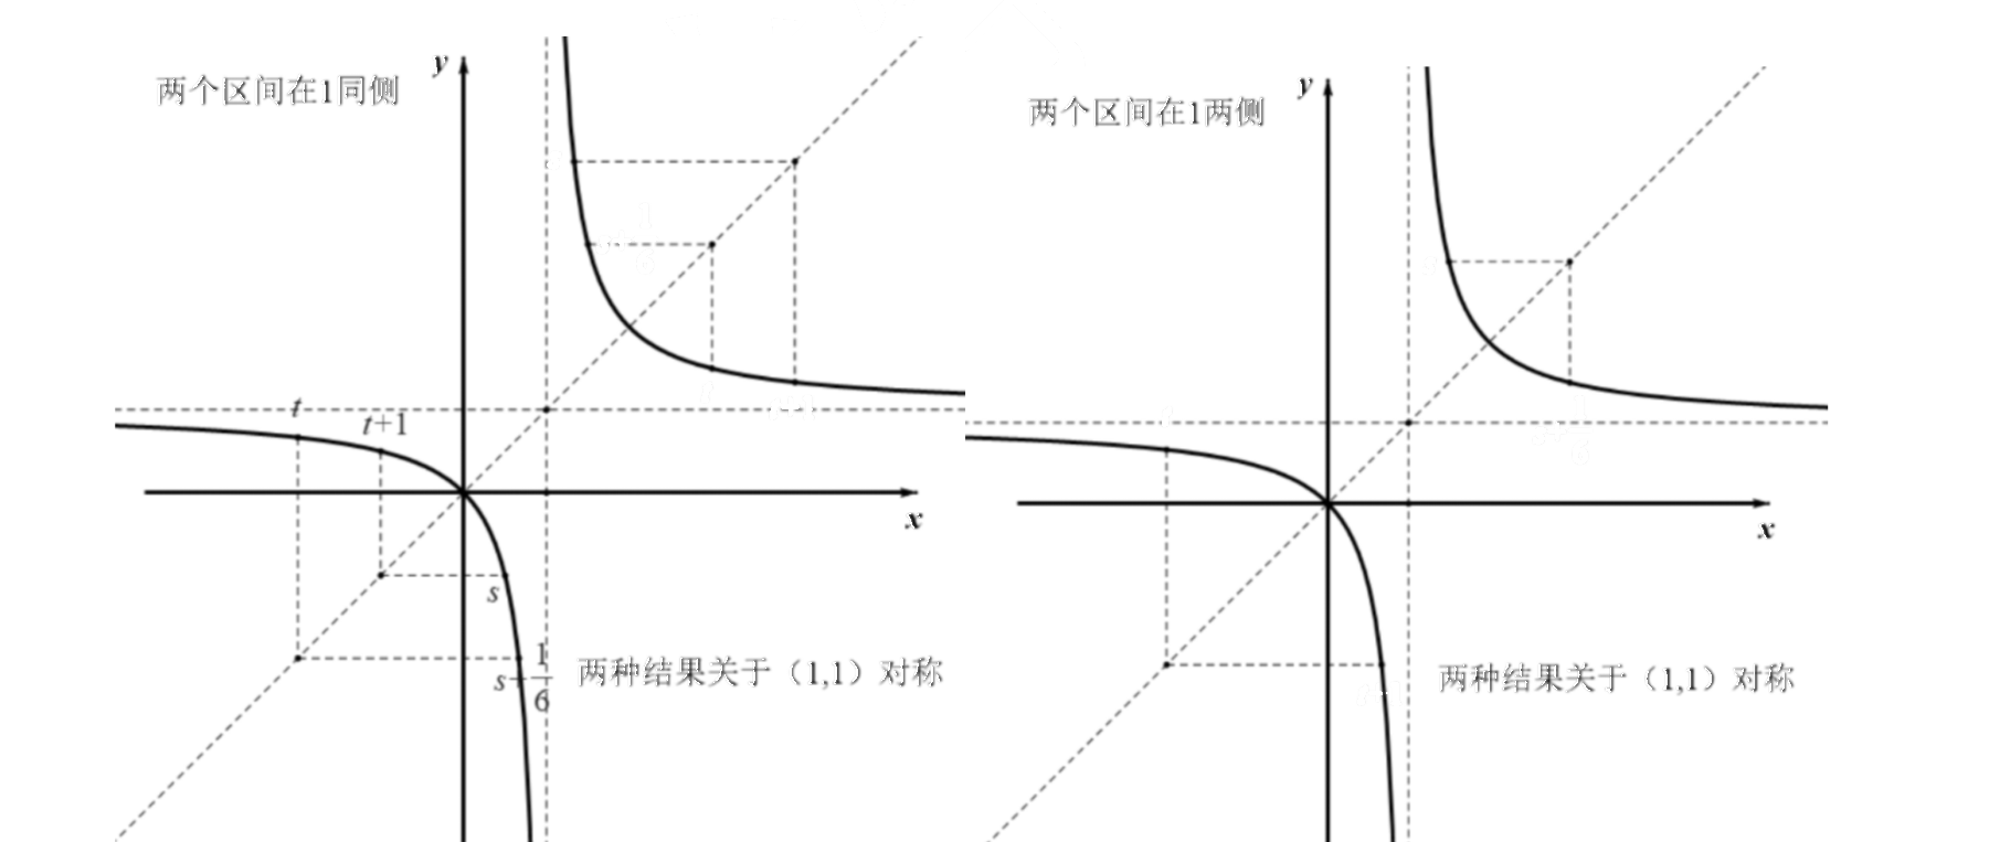
\includegraphics[width=0.92\textwidth]{figures/gao115_q10.png}
\end{center}
\solend
\fi

\end{enumerate}

\bigsec{二、选择题}

\begin{enumerate}
\setcounter{enumi}{10}

\item “对任意有理数 $x$ 都有 $x^2\neq2$”的否定形式是\mbox{（\quad）}% 原卷把答案“$B$”印在题干括号内、无【解析】

\keepwithprev
A. 存在有理数 $x$ 使得 $x^2\neq2$\qquad\qquad B. 存在有理数 $x$ 使得 $x^2=2$

C. 存在无理数 $x$ 使得 $x^2\neq2$\qquad\qquad D. 存在无理数 $x$ 使得 $x^2=2$

\ifanswer
\ans{$B$}
\fi

\item 已知 $a$、$b$ 都是实数，那么“$a^3>b^3$”是“$a^2>b^2$”的\mbox{（\quad）}

\keepwithprev
A. 充分不必要条件\qquad\qquad B. 必要不充分条件

C. 充要条件\qquad\qquad\qquad D. 既不充分也不必要条件

\ifanswer
\solbegin
\step{因为 $a^3>b^3$ 等价于 $a>b$，}
\step{由于 $a$、$b$ 正负不定，所以由 $a>b$ 不能得到 $a^2>b^2$，}
\step{由 $a^2>b^2$ 也不能得到 $a>b$，}
\step{因此“$a^3>b^3$”是“$a^2>b^2$”的既不充分也不必要条件. 故选 $D$.}
\solend
\fi

\item 定义集合运算 $A-B=\{x\mid x\in A$ 且 $x\notin B\}$，将 $A\triangle B=(A-B)\cup(B-A)$ 称为集合 $A$ 与集合 $B$ 的对称差.

命题一：$A\triangle B=B\triangle A$；

命题二：$A\triangle\varnothing=A$；

命题三：$A\cap(B\triangle C)=(A\cap B)\triangle(A\cap C)$；

命题四：$A\cup(B\triangle C)=(A\cup B)\triangle(A\cup C)$；

其中正确命题的个数是\mbox{（\quad）}

\keepwithprev
A. $1$\qquad\qquad B. $2$\qquad\qquad C. $3$\qquad\qquad D. $4$

\ifanswer
\solbegin
\step{对于①，$B\triangle A=(B-A)\cup(A-B)=(A-B)\cup(B-A)=A\triangle B$，①对；}
\step{对于②，$A-B=\{x\mid x\in A$ 且 $x\notin B\}=\{x\mid x\in A$ 且 $x\notin(A\cap B)\}$}
\step{$=A-(A\cap B)$，则 $A\triangle\varnothing=(A-\varnothing)\cup(\varnothing-A)=A\cup\varnothing=A$，②对；}
\step{对于③，$A\cap(B\triangle C)=A\cap(B\cup C-B\cap C)=A\cap(B\cup C)-A\cap(B\cap C)$}
\step{$=(A\cap B)\cup(A\cap C)-(A\cap B)\cap(A\cap C)=(A\cap B)\triangle(A\cap C)$，③对；}
\step{对于④，如图所示：}
\begin{center}
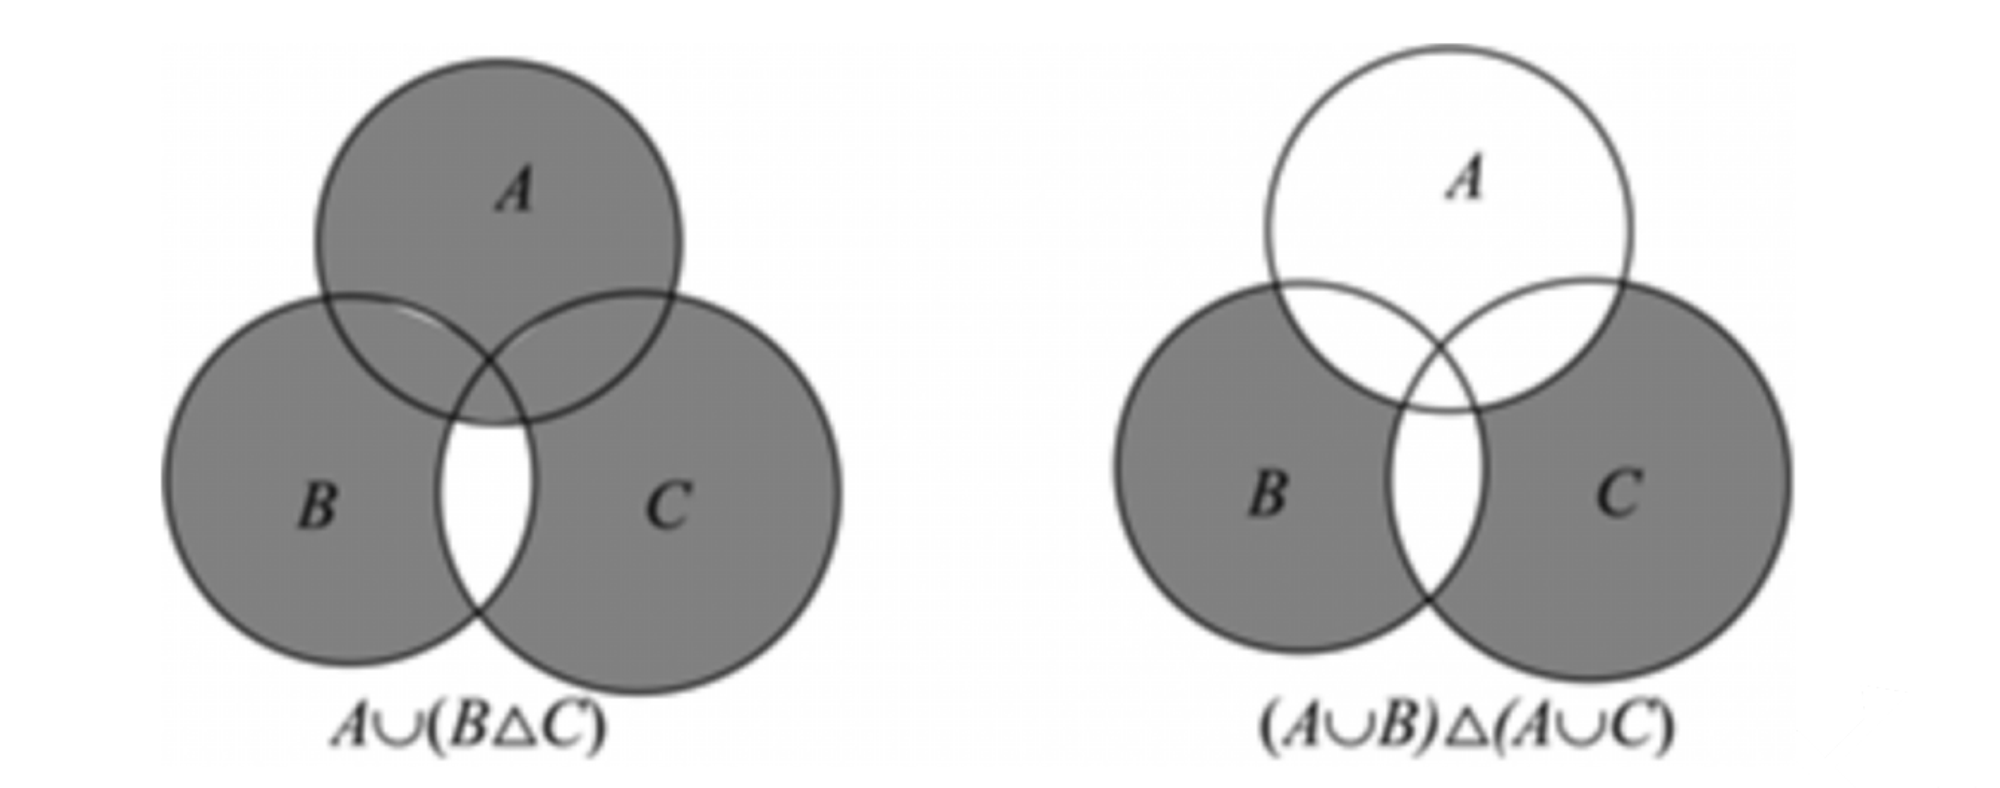
\includegraphics[width=0.85\textwidth]{figures/gao115_q13.png}
\end{center}
\step{所以 $A\cup(B\triangle C)\neq(A\cup B)\triangle(A\cup C)$，④错.}
\step{故选 $C$.}
\solend
\fi

\item 设 $a$、$b$、$c$、$p$ 为实数，若同时满足不等式 $ax^2+bx+c>0$、$bx^2+cx+a>0$ 与 $cx^2+ax+b>0$ 的全体实数 $x$ 所组成的集合等于 $(p,+\infty)$，则关于结论：① $a$、$b$、$c$ 至少有一个为 $0$；② $p=0$. 下列判断中正确的是\mbox{（\quad）}

\keepwithprev
A. ①和②都正确\qquad B. ①和②都错误\qquad C. ①正确，②错误\qquad D. ①错误，②正确

\ifanswer
\solbegin
\step{若同时满足不等式 $ax^2+bx+c>0$、$bx^2+cx+a>0$ 与 $cx^2+ax+b>0$ 的}
\step{全体实数 $x$ 所组成的集合等于 $(p,+\infty)$，必有 $a$,$b$,$c\geqslant0$，}
\step{不妨假设 $a$、$b$、$c$ 没有一个为 $0$，}
\step{则三个不等式均为开口向上的二次函数大于 $0$ 的部分，}
\step{解集的交集应为 $(-\infty,m)\cup(n,+\infty)$ 的形式，矛盾，}
\step{所以 $a$、$b$、$c$ 至少有一个为 $0$，故①正确：}
\step{不妨设 $a=0$，则 $b$,$c\geqslant0$，则不等式组化为 $\begin{cases}bx+c>0\\bx^2+cx>0,\\cx^2+b>0\end{cases}$}
\step{所以 $\begin{cases}x>-\dfrac cb\\x<-\dfrac cb\text{或}x>0\\x\in\R\end{cases}$，取交集得 $(0,+\infty)$，故 $p=0$，故②正确：}
\step{故选 $A$.}
\solend
\fi

\end{enumerate}

\bigsec{三、解答题}

\begin{enumerate}
\setcounter{enumi}{14}

\item 已知 $a>0$，$b>0$，

（1）试比较 $\dfrac{a^2-b^2}{a^2+b^2}$ 与 $\dfrac{a-b}{a+b}$ 的大小；

（2）若 $a+b>4$，求证：$\dfrac a{b+2}$ 和 $\dfrac b{a+2}$ 中至少有一个大于 $\dfrac12$.

\ifanswer
\solbegin
\step{（1）已知 $a>0$，$b>0$，$\dfrac{a^2-b^2}{a^2+b^2}-\dfrac{a-b}{a+b}=\dfrac{2ab(a-b)}{(a^2+b^2)(a+b)}$，}
\step{当 $a>b$ 时，$a-b>0$，所以 $\dfrac{a^2-b^2}{a^2+b^2}-\dfrac{a-b}{a+b}>0$，所以 $\dfrac{a^2-b^2}{a^2+b^2}>\dfrac{a-b}{a+b}$；}
\step{当 $a=b$ 时，$a-b=0$，所以 $\dfrac{a^2-b^2}{a^2+b^2}-\dfrac{a-b}{a+b}=0$，所以 $\dfrac{a^2-b^2}{a^2+b^2}=\dfrac{a-b}{a+b}$；}
\step{当 $a<b$ 时，$a-b<0$，所以 $\dfrac{a^2-b^2}{a^2+b^2}-\dfrac{a-b}{a+b}<0$，所以 $\dfrac{a^2-b^2}{a^2+b^2}<\dfrac{a-b}{a+b}$；}
\step{（2）假设 $\dfrac a{b+2}$ 和 $\dfrac b{a+2}$ 中都不大于 $\dfrac12$，即 $\dfrac b{a+2}\leqslant\dfrac12$，$\dfrac a{b+2}\leqslant\dfrac12$，}
\step{因为 $a>0$，$b>0$，所以 $a+2>0$，$b+2>0$，}
\step{所以 $2b\leqslant a+2$，$2a\leqslant b+2$，}
\step{两式相加得 $2a+2b\leqslant a+2+b+2=a+b+4$，即 $a+b\leqslant4$，}
\step{与已知 $a+b>4$ 矛盾，所以假设错误，}
\step{故 $\dfrac a{b+2}$ 和 $\dfrac b{a+2}$ 中至少有一个大于 $\dfrac12$.}
\solend
\fi

\item 某企业原有 $200$ 名科技人员，年人均工资 $a$ 万元($a>0$). 现加大对某芯片研发力度，该企业把原有 $200$ 名科技人员调整成技术人员和研发人员，其中技术人员 $x$ 名($x\in\N$ 且 $40\leqslant x\leqslant80$). 调整后，研发人员的年人均工资比调整前增加了 $(2x)\%$，技术人员的年人均工资为 $a\left(m-\dfrac x{10}\right)$万元.

（1）若要使调整后研发人员的年总工资不低于调整前 $200$ 名科技人员年总工资的 $1.5$ 倍，求调整后的技术人员最少有多少人？

（2）为了激励研发人员的工作热情和保持技术人员的工作积极性，企业决定在工资方面要同时满足以下两个条件：

①研发人员的年总工资始终不低于技术人员的年总工资；

②技术人员的年人均工资始终不低于调整前 $200$ 名科技人员的年人均工资.

请问是否存在这样的实数 $m$？若存在，求出 $m$ 的范围；若不存在，说明理由.

\ifanswer
\solbegin
\step{（1）由题意得调整后研发人员的年人均工资为 $[1+(2x)\%]a$ 万元，}
\step{那么 $(200-x)[1+(2x)\%]a\geqslant1.5\times200a$ ($a>0$)，}
\step{化简得 $x^2-150x+5000\leqslant0$，解得 $50\leqslant x\leqslant100$，}
\step{由于 $x\in\N$ 且 $40\leqslant x\leqslant80$，因此 $50\leqslant x\leqslant80$，}
\step{因此调整后的技术人员的人数最少为 $50$ 人；}
\step{（2）假设存在实数 $m$，使得技术人员在已知范围内调整后，满足以上两个条件，}
\step{由条件①得 $(200-x)[1+(2x)\%]a\geqslant x\left(m-\dfrac x{10}\right)a$，}
\step{整理得 $m\leqslant\dfrac{200}{x}+\dfrac{2x}{25}+3$；}
\step{因为 $\dfrac{200}{x}+\dfrac{2x}{25}+3\geqslant2\sqrt{\dfrac{200}{x}\cdot\dfrac{2x}{25}}+3=11$，}
\step{当且仅当 $\dfrac{200}{x}=\dfrac{2x}{25}$，即 $x=50$ 时取等号，因此 $m\leqslant11$，}
\step{由条件②得 $a\left(m-\dfrac x{10}\right)\geqslant a$，所以 $m\geqslant\dfrac x{10}+1$；}
\step{又由于 $40\leqslant x\leqslant80$，因此 $m\geqslant9$.}
\step{因此 $m\in[9,11]$.}
\solend
\fi

\item 已知 $a\in\R$，记 $f(x)=ax^2-(a+2)x+2$.

（1）若 $f(x)<3-2x$ 对于一切 $x\in\R$ 恒成立，求实数 $a$ 的取值范围；

（2）求关于 $x$ 不等式 $f(x)\geqslant0$ 的解集；

（3）若存在 $m\in\R$ 使关于 $x$ 的方程 $ax^2-(a+2)\lvert x\rvert+2=\lvert m+2\rvert+\lvert m-1\rvert$ 有四个不同的实根，求实数 $a$ 的取值范围.

\ifanswer
\solbegin
\step{（1）由 $f(x)<3-2x$ 对于一切 $x\in\R$ 恒成立，}
\step{得 $ax^2-ax-1<0$ 对于一切 $x\in\R$ 恒成立，}
\step{当 $a=0$ 时，原式可化为 $-1<0$，恒成立，符合条件；}
\step{当 $a\neq0$ 时，需满足 $\begin{cases}a<0\\\Delta=a^2+4a<0\end{cases}$，解得 $-4<a<0$；}
\step{综上，实数 $a$ 的取值范围是 $(-4,0]$；}
\step{（2）$f(x)\geqslant0$，即 $(ax-2)(x-1)\geqslant0$，}
\step{当 $a=0$ 时，原式化为 $-2x+2\geqslant0$，解集为 $\{x\mid x\leqslant1\}$；}
\step{当 $a>0$ 时，若 $a=2$，原式化为 $2(x-1)^2\geqslant0$，解集为 $\R$；}
\step{若 $0<a<2$，$\dfrac2a>1$，解集为 $\{x\mid x\leqslant1$ 或 $x\geqslant\dfrac2a\}$；}
\step{若 $a>2$，$\dfrac2a<1$，解集为 $\{x\mid x\leqslant\dfrac2a$ 或 $x\geqslant1\}$；}
\step{当 $a<0$ 时，$\dfrac2a<1$，解集为 $\left\{x\,\middle\vert\,\dfrac2a\leqslant x\leqslant1\right\}$；}
\step{综上，当 $a<0$ 时，不等式解集为 $\left\{x\,\middle\vert\,\dfrac2a\leqslant x\leqslant1\right\}$；}
\step{当 $a=0$ 时，不等式解集为 $\{x\mid x\leqslant1\}$；}
\step{当 $0<a<2$ 时，不等式解集为 $\{x\mid x\leqslant1$ 或 $x\geqslant\dfrac2a\}$；}
\step{当 $a=2$ 时，不等式解集为 $\R$；}
\step{当 $a>2$ 时，不等式解集为 $\{x\mid x\leqslant\dfrac2a$ 或 $x\geqslant1\}$；}
\step{（3）由绝对值三角不等式得 $\lvert m+2\rvert+\lvert m-1\rvert\geqslant\lvert(m+2)-(m-1)\rvert=3$，}
\step{即右侧取值范围为 $[3,+\infty)$，}
\step{令 $t=\lvert x\rvert\geqslant0$，原方程转化为 $at^2-(a+2)t+2=k$，$k\in[3,+\infty)$，}
\step{若原方程有四个不同实根，}
\step{需存在 $k\geqslant3$，使得方程 $at^2-(a+2)t+2-k=0$ 有两个不同正实根，}
\step{当 $a\geqslant0$ 时，方程的两根之积为 $\dfrac{2-k}{a}$，}
\step{因为 $k\geqslant3$，所以 $2-k\leqslant-1<0$，两根一正一负，}
\step{最多只有一个正根，对应最多两个 $x$ 根，不符合要求；}
\step{当 $a<0$ 时，两根之积为正，}
\step{要两个根都为正，需要两根之和 $\dfrac{a+2}{a}>0$，解得 $a<-2$，}
\step{再要求存在 $k\geqslant3$ 使得判别式大于 $0$，}
\step{即 $\triangle=(a+2)^2-4a(2-k)>0$ 在 $k\in[3,+\infty)$ 上有解，}
\step{即 $(a-2)^2+4ak>0$ 在 $k\in[3,+\infty)$ 上有解，}
\step{由 $a<0$，得 $(a-2)^2+12a>0$，}
\step{即 $a^2+8a+4>0$，结合 $a<-2$ 解得 $a<-4-2\sqrt3$，}
\step{故实数 $a$ 的取值范围是 $(-\infty,-4-2\sqrt3)$.}
\solend
\fi

\item 设 $A=\{x_1,x_2,\cdots,x_n\}(n\geqslant2,n\in\N)$，且 $x_1,x_2,\cdots,x_n$ 均为正整数，若对于 $A$ 中任意两个元素 $a,b$，当 $a>b$ 时，都有 $\dfrac{b^2}{a-b}\in A$，则称 $A$ 为“$n$ 元好集”.

（1）判断 $\{2,4,6\}$ 是否为“三元好集”，并说明理由；

（2）若集合 $M$ 为“二元好集”，且 $M$ 中所有元素之积小于 $2026$，求所有满足条件的集合 $M$ 的个数；

（3）设 $k\geqslant3,k\in\N$，是否存在“$k$ 元好集”，若存在，求出所有满足条件的“$k$ 元好集”，若不存在，请说明理由.

\ifanswer
\solbegin
\step{（1）取 $a=6,b=2$，则 $\dfrac{b^2}{a-b}=\dfrac44=1\notin\{2,4,6\}$，所以该集合不是三元好集.}
\step{（2）设 $M=\{b,a\}$，其中 $a>b$ 且均为正整数，则 $\dfrac{b^2}{a-b}$ 等于 $a$ 或 $b$.}
\step{若 $\dfrac{b^2}{a-b}=a$，则 $a^2-ab-b^2=0$，从而 $\dfrac ab=\dfrac{1+\sqrt5}{2}$，与 $\dfrac ab$ 为有理数矛盾.}
\step{若 $\dfrac{b^2}{a-b}=b$，则 $a=2b$；}
\step{反之，任意正整数 $b$ 对应的 $\{b,2b\}$ 均为二元好集.}
\step{由元素之积小于 $2026$，得 $2b^2<2026\Leftrightarrow b^2<1013$.}
\step{因为 $31^2=961<1013<1024=32^2$，所以 $b=1,2,\cdots,31$，}
\step{对应 $31$ 个不同的集合.}
\step{（3）假设存在 $k\geqslant3$ 的 $k$ 元好集 $A$，将其元素从小到大排列，}
\step{记最小元素为 $u$，次小元素为 $v$，最大元素为 $w$，则 $0<u<v<w$.}
\step{由 $\dfrac{u^2}{w-u}\in A$，该数不小于 $u$，得 $\dfrac{u^2}{w-u}\geqslant u\Rightarrow w\leqslant2u$.}
\step{又由 $\dfrac{u^2}{v-u}$,$\dfrac{v^2}{w-v}\in A$，这两个数均不超过 $w$，}
\step{得 $\dfrac{u^2}{v-u}\leqslant w$,$\dfrac{v^2}{w-v}\leqslant w$，}
\step{分母均为正，分别去分母后相加，}
\step{得 $u^2+v^2\leqslant w(v-u)+w(w-v)=w(w-u)\leqslant2u^2$，}
\step{于是 $v^2\leqslant u^2$，与 $v>u>0$ 矛盾，所以不存在 $k\geqslant3$ 的 $k$ 元好集.}
\solend
\fi

\end{enumerate}

\end{document}
"
%
% 原始材料：微信公众号“魔都数学加油站”文章，作者破晓，2026-11-06 17:58 发布；
% 连载“27学年高一115”，原文标题“27学年高一115——2026-2027年上海市复旦附中高一上10月阶段练习”；
% 原文链接：https://mp.weixin.qq.com/s/krocP0fMQQ4VM1SQEcLI2Q。
% 正文为 12 张 PNG 页（第 4、6、12 页 2560×3620，其余 4762×6735），
% 题目下印有【解析】或【答案】，为讲评版。
% 题目、解析均据原图转录；卷面红色水印及公众号页脚未录入。
%
% 卷首标题：原卷印作“2026-2027 年复旦附中高一上 10 月阶段练习”（公众号标题中的“上海市”
% 卷面标题行没有，本稿照卷面），年份区间按全稿惯例排 en dash；原卷未印副标题，本稿按题目内容
% 标为“集合与常用逻辑用语、不等式”。
%
% 与原卷的排版差异：
%   ① 原文从第 3 题起，填空题编号为 3—10、选择题为 11—14、解答题为 15—18，共 16 题，
%      本稿保留原题号（与多数卷的 3—21 不同）；
%   ② 原卷每题下直接印【解析】／【答案】，本稿按全稿惯例置于答案版；第 11 题把答案“$B$”
%      印在题干括号内且无【解析】，另提 \ans{}；其余选择题答案在解析末句“故选 …”，括号内留空；
%   ③ 原卷未印副标题，本稿按“知识模块”口径补出；
%   ④ 原卷填空横线按全稿惯例排为 \blankline[4.4em]；选择题括号排 \mbox{（\quad）}、
%      选项段前按惯例加 \keepwithprev；解答题不留作答区（原卷为讲评版，与 109—114 同）；
%   ⑤ 原卷数集排斜体 $R$／$Q$／$N$，按全稿惯例改 \R、\Q、\N。
%
% 判别式与对称差字形：原卷 $\triangle$（等边、扁）与 $\Delta$（等腰、高）两种混用，逐处照录——
%   第 7 题与第 17 题 (3) 的判别式、第 13 题的对称差 $A\triangle B$ 用 \triangle，
%   第 17 题 (1) cases 的判别式用 \Delta。
%
% 子集符号：第 4 题解析的 $(-1,3)\subset(-m,m)$ 印单线（真子集、无下划线），按 18／96
%   成例照录 \subset；第 5 题解析的 $B\subseteq A$ 印有下划线，照录 \subseteq。
%   第 3 题的补集照原卷上划线排 \overline{N}。
%
% 原卷存疑照录：第 9 题解析末行“故可能成立的是①②③”与四种情形的编号一致，照录；
%   第 10 题解析两幅函数图上另有蓝色／红色手写标注（$t$、$t+1$、$s$、$\frac16$ 等），
%   系批改笔迹，随裁图保留、不另作正文录入；第 14 题解析的 cases 三行照原卷排；
%   第 18 题 (2) 解析“所以该集合不是三元好集”前的取例 $a=6,b=2$ 照录。
%
% 行数核对：逐题数 \step/\stepm 条数，合计 133 条（Q3：3；Q4：3；Q5：4；Q6：5；Q7：4；
% Q8：4；Q9：11；Q10：7；Q11：0；Q12：4；Q13：8；Q14：9；Q15：10；Q16：13；
% Q17：32；Q18：16），与原卷印刷行逐题相等（cases 块作一个印刷行计）。第 11 题括号内印
% 答案且无解析，提 \ans{}，不计入 \step 账；第 10、13 题解析内的插图不计入 \step 账。
%
\documentclass[a4paper,11pt]{article}
\usepackage{common}

\begin{document}

\examtitlest[3]{2026--2027 年复旦附中高一上 10 月阶段练习}{集合与常用逻辑用语、不等式}

\bigsec{一、填空题}

\begin{enumerate}
\setcounter{enumi}{2}

\item 已知集合 $M=\{x\mid 4x^2-4x-15>0\}$，$N=\left\{x\,\middle\vert\,\dfrac{x+1}{x-6}>0\right\}$，则 $M\cap\overline{N}=$\blankline[4.4em].

\ifanswer
\solbegin
\step{集合 $M=\{x\mid 4x^2-4x-15>0\}=\{x\mid x>\dfrac52$ 或 $x<-\dfrac32\}$，}
\step{$N=\left\{x\,\middle\vert\,\dfrac{x+1}{x-6}>0\right\}=\{x\mid x>6$ 或 $x<-1\}$，得 $\overline{N}=\{x\mid-1\leqslant x\leqslant6\}$，}
\step{故 $M\cap\overline{N}=\left\{x\,\middle\vert\,\dfrac52<x\leqslant6\right\}$.}
\solend
\fi

\item 已知 $m>0$，不等式 $\lvert x\rvert<m$ 成立的一个充分不必要条件是 $-1<x<3$，则 $m$ 的取值范围是\blankline[4.4em].

\ifanswer
\solbegin
\step{不等式 $-m<x<m$ 成立的一个充分不必要条件是 $-1<x<3$，}
\step{由题意得 $(-1,3)\subset(-m,m)$，则 $m\geqslant3$，此时 $-m\leqslant-3<-1$，}% 原卷印单线 \subset，照录
\step{所以 $m$ 的取值范围是 $\{m\mid m\geqslant3\}$.}
\solend
\fi

\item 已知集合 $A=\{1,2\}$，集合 $B=\{x\mid ax=6\}$，若 $A\cup B=A$，则 $a$ 的所有取值构成的集合为\blankline[4.4em].

\ifanswer
\solbegin
\step{因为 $A\cup B=A$，所以 $B\subseteq A$，}
\step{当 $a=0$ 时，$B=\varnothing$，满足 $B\subseteq A$；}
\step{当 $a\neq0$ 时，$B=\left\{\dfrac6a\right\}$，则 $\dfrac6a=1$ 或 $\dfrac6a=2$，解得 $a=6$ 或 $a=3$，}
\step{综上所述，$a$ 的所有取值构成的集合为 $\{0,3,6\}$.}
\solend
\fi

\item 若关于 $x$ 的不等式 $ax^2+bx+c>0$ 的解集为 $(-3,2)$，则不等式 $ax^2+(a+b)x+c-2a>0$ 的解集为\blankline[4.4em].

\ifanswer
\solbegin
\step{由 $ax^2+bx+c>0$ 的解集为 $(-3,2)$ 得 $a<0$，}
\step{且 $ax^2+bx+c=0$ 时 $x_1=-3$，$x_2=2$，}
\step{得 $-3+2=-\dfrac ba$，即 $b=a$，$-3\times2=\dfrac ca$，即 $c=-6a$，}
\step{代入 $ax^2+(a+b)x+c-2a>0$ 得 $ax^2+2ax-8a>0$ 化简得 $x^2+2x-8<0$，}
\step{解得 $-4<x<2$，故解集为 $(-4,2)$.}
\solend
\fi

\item 已知关于 $x$ 的方程 $x^2-2x+m=0$ 的两个实数根分别为 $x_1$，$x_2$. 若 $x_1^2x_2^2+x_1^2+x_2^2=7$，则实数 $m$ 的值为\blankline[4.4em].

\ifanswer
\solbegin
\step{由韦达定理得 $x_1+x_2=2$，$x_1x_2=m$，}
\step{$x_1^2x_2^2+x_1^2+x_2^2=(x_1x_2)^2+(x_1+x_2)^2-2x_1x_2=m^2+4-2m$，}
\step{由 $m^2+4-2m=7$，得 $m^2-2m-3=0$，解得 $m=3$ 或 $m=-1$，}
\step{方程有两个实数根，故 $\triangle=4-4m\geqslant0$，即 $m\leqslant1$，所以 $m=-1$.}
\solend
\fi

\item 已知 $x>1$，若 $x^2-xy+y=0$，则 $x+y$ 的最小值是\blankline[4.4em].

\ifanswer
\solbegin
\step{由于 $x^2-xy+y=0$，则 $y=\dfrac{x^2}{x-1}>0$，}
\step{则 $x+y=x+\dfrac{x^2}{x-1}=\dfrac{2x^2-x}{x-1}=\dfrac{2(x-1)^2+3(x-1)+1}{x-1}$}
\step{$=2(x-1)+\dfrac1{x-1}+3\geqslant2\sqrt{2(x-1)\cdot\dfrac1{x-1}}+3=2\sqrt2+3$，}
\step{当且仅当 $x=1+\dfrac{\sqrt2}{2}$ 时取等号，故最小值是 $2\sqrt2+3$.}
\solend
\fi

\item 若集合 $A=B_1\cup B_2\cup\cdots\cup B_n$，其中 $B_1$、$B_2$、$\cdots$、$B_n$ 为非空集合，$B_i\cap B_j=\varnothing$，$1\leqslant i<j\leqslant n$，则称集合 $\{B_1,B_2,\cdots,B_n\}$ 为集合 $A$ 的一个 $n$ 划分. 例如：集合 $\{\{1,2\},\{3\}\}$，$\{\{1,3\},\{2\}\}$，$\{\{2,3\},\{1\}\}$ 均为集合 $\{1,2,3\}$ 的一个 $2$ 划分. 设 $\{B_1,B_2\}$ 为有理数集 $\Q$ 的一个 $2$ 划分，且满足对任意 $x\in B_1$，任意 $y\in B_2$，都有 $x<y$. 则对于 $B_1$、$B_2$ 有：

① $B_1$ 中的元素存在最大值，$B_2$ 中的元素不存在最小值；

② $B_1$ 中的元素不存在最大值，$B_2$ 中的元素存在最小值；

③ $B_1$ 中的元素不存在最大值，$B_2$ 中的元素不存在最小值；

④ $B_1$ 中的元素存在最大值，$B_2$ 中的元素存在最小值；

对于以上四种情况，可能成立的序号有\blankline[4.4em].

\ifanswer
\solbegin
\step{对于①，$B_1=\{x\in\Q\mid x\leqslant2\}$，$B_2=\{x\in\Q\mid x>2\}$，①可能成立；}
\step{对于②，$B_1=\{x\in\Q\mid x<2\}$，$B_2=\{x\in\Q\mid x\geqslant2\}$，②可能成立；}
\step{对于③，$B_1=\{x\in\Q\mid x<\pi\}$，$B_2=\{x\in\Q\mid x>\pi\}$，③可能成立；}
\step{对于④，假设④成立，}
\step{不妨设 $B_1$ 中的元素的最大值为 $s$，$B_2$ 中的元素的最小值为 $t$，}
\step{由题意得 $s<t$，所以 $s<\dfrac{s+t}{2}<t$，}
\step{因为 $s$ 为 $B_1$ 中的元素的最大值，所以 $\dfrac{s+t}{2}\notin B_1$，}
\step{因为 $t$ 为 $B_2$ 中的元素的最小值，所以 $\dfrac{s+t}{2}\notin B_2$，}
\step{又 $B_1\cup B_2=\Q$，所以 $\dfrac{s+t}{2}\notin\Q$，与 $\dfrac{s+t}{2}\in\Q$ 矛盾，}
\step{所以假设不成立，即④不可能成立.}
\step{故可能成立的是①②③.}
\solend
\fi

\item 已知集合 $A=\left[s,s+\dfrac16\right]\cup[t,t+1]$，其中 $1\notin A$ 且 $s+\dfrac16<t$，函数 $f(x)=\dfrac x{x-1}$，且对任意 $a\in A$，都有 $f(a)\in A$，则 $t$ 的值是\blankline[4.4em].

\ifanswer
\solbegin
\step{若 $\left[s,s+\dfrac16\right]$,$[t,t+1]$ 在 $f(x)=\dfrac x{x-1}$ 图像的同侧，}
\step{则点 $\left(t,s+\dfrac16\right)$,$(t+1,s)$ 在 $f(x)=\dfrac x{x-1}$ 的图像上，}
\step{所以 $\dfrac t{t-1}=\dfrac{t+1}{t}+\dfrac16$，解得 $t=-2$ 或 $t=3$，检验得 $t=3$；}
\step{若 $\left[s,s+\dfrac16\right]$,$[t,t+1]$ 在 $f(x)=\dfrac x{x-1}$ 图像的两侧，}
\step{则点 $(t,t+1)$ 在 $f(x)=\dfrac x{x-1}$ 的图像上，}
\step{所以 $t+1=\dfrac t{t-1}$，解得 $t=\dfrac{1\pm\sqrt5}{2}$，检验得 $t=\dfrac{1+\sqrt5}{2}$，}
\step{综上，$t=\dfrac{1+\sqrt5}{2}$ 或 $t=3$.}
\begin{center}
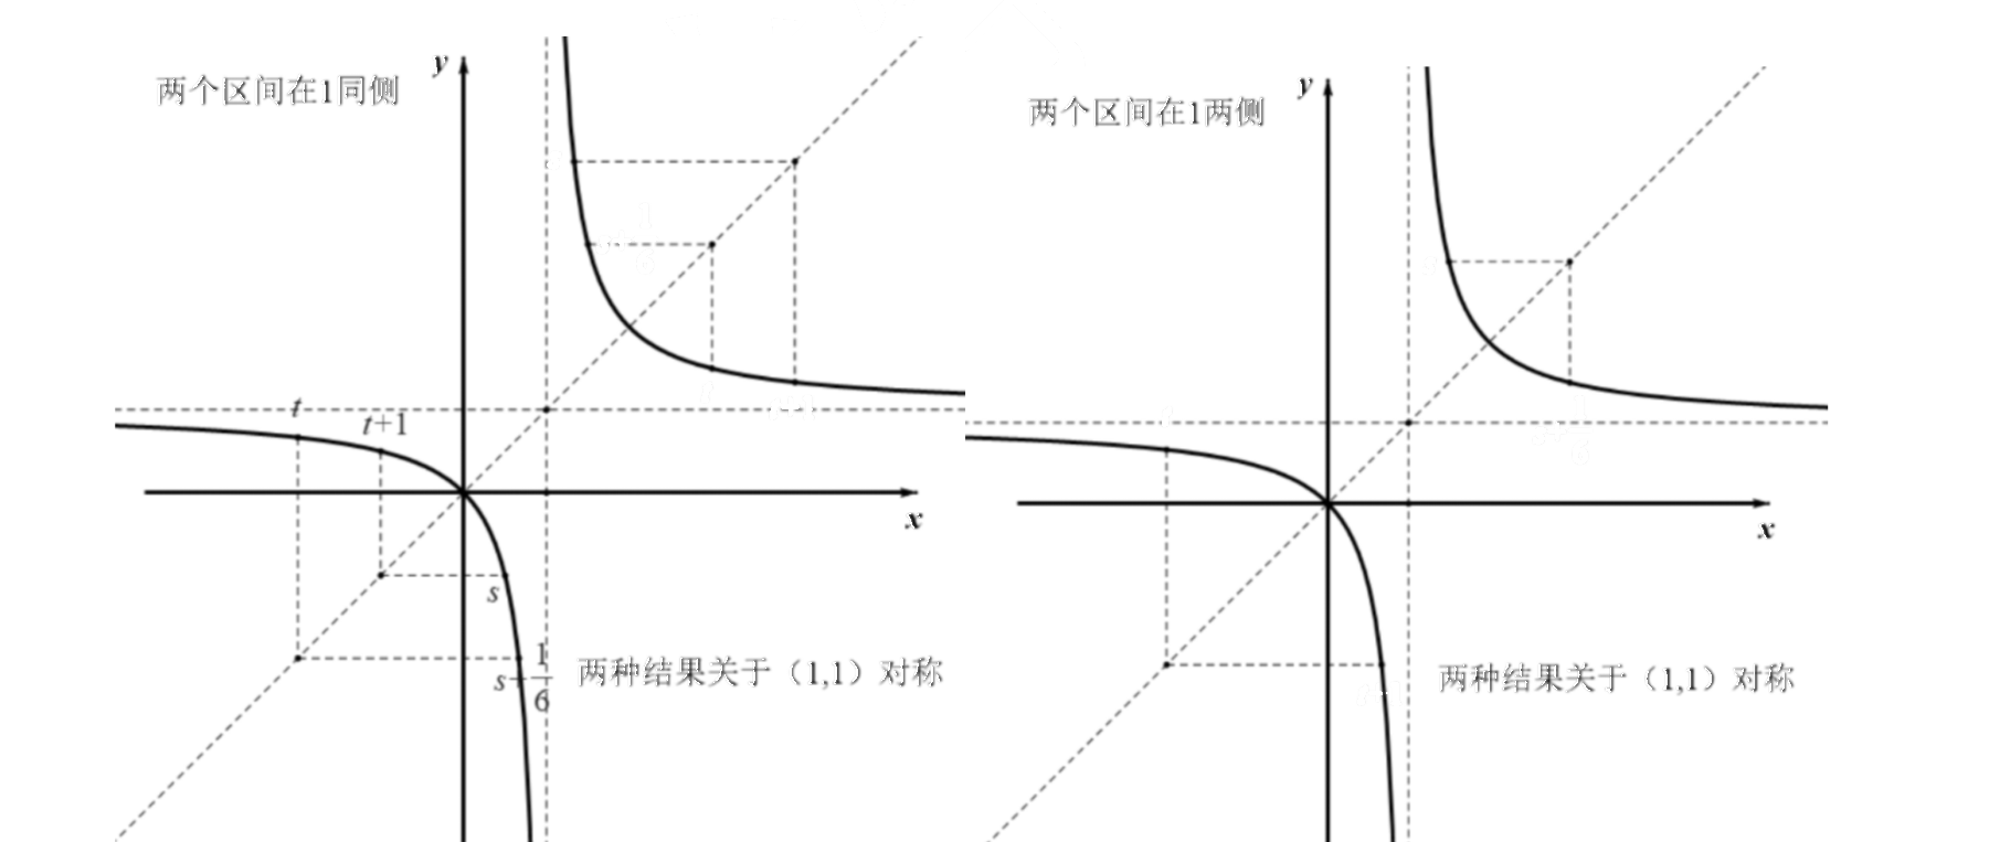
\includegraphics[width=0.92\textwidth]{figures/gao115_q10.png}
\end{center}
\solend
\fi

\end{enumerate}

\bigsec{二、选择题}

\begin{enumerate}
\setcounter{enumi}{10}

\item “对任意有理数 $x$ 都有 $x^2\neq2$”的否定形式是\mbox{（\quad）}% 原卷把答案“$B$”印在题干括号内、无【解析】

\keepwithprev
A. 存在有理数 $x$ 使得 $x^2\neq2$\qquad\qquad B. 存在有理数 $x$ 使得 $x^2=2$

C. 存在无理数 $x$ 使得 $x^2\neq2$\qquad\qquad D. 存在无理数 $x$ 使得 $x^2=2$

\ifanswer
\ans{$B$}
\fi

\item 已知 $a$、$b$ 都是实数，那么“$a^3>b^3$”是“$a^2>b^2$”的\mbox{（\quad）}

\keepwithprev
A. 充分不必要条件\qquad\qquad B. 必要不充分条件

C. 充要条件\qquad\qquad\qquad D. 既不充分也不必要条件

\ifanswer
\solbegin
\step{因为 $a^3>b^3$ 等价于 $a>b$，}
\step{由于 $a$、$b$ 正负不定，所以由 $a>b$ 不能得到 $a^2>b^2$，}
\step{由 $a^2>b^2$ 也不能得到 $a>b$，}
\step{因此“$a^3>b^3$”是“$a^2>b^2$”的既不充分也不必要条件. 故选 $D$.}
\solend
\fi

\item 定义集合运算 $A-B=\{x\mid x\in A$ 且 $x\notin B\}$，将 $A\triangle B=(A-B)\cup(B-A)$ 称为集合 $A$ 与集合 $B$ 的对称差.

命题一：$A\triangle B=B\triangle A$；

命题二：$A\triangle\varnothing=A$；

命题三：$A\cap(B\triangle C)=(A\cap B)\triangle(A\cap C)$；

命题四：$A\cup(B\triangle C)=(A\cup B)\triangle(A\cup C)$；

其中正确命题的个数是\mbox{（\quad）}

\keepwithprev
A. $1$\qquad\qquad B. $2$\qquad\qquad C. $3$\qquad\qquad D. $4$

\ifanswer
\solbegin
\step{对于①，$B\triangle A=(B-A)\cup(A-B)=(A-B)\cup(B-A)=A\triangle B$，①对；}
\step{对于②，$A-B=\{x\mid x\in A$ 且 $x\notin B\}=\{x\mid x\in A$ 且 $x\notin(A\cap B)\}$}
\step{$=A-(A\cap B)$，则 $A\triangle\varnothing=(A-\varnothing)\cup(\varnothing-A)=A\cup\varnothing=A$，②对；}
\step{对于③，$A\cap(B\triangle C)=A\cap(B\cup C-B\cap C)=A\cap(B\cup C)-A\cap(B\cap C)$}
\step{$=(A\cap B)\cup(A\cap C)-(A\cap B)\cap(A\cap C)=(A\cap B)\triangle(A\cap C)$，③对；}
\step{对于④，如图所示：}
\begin{center}
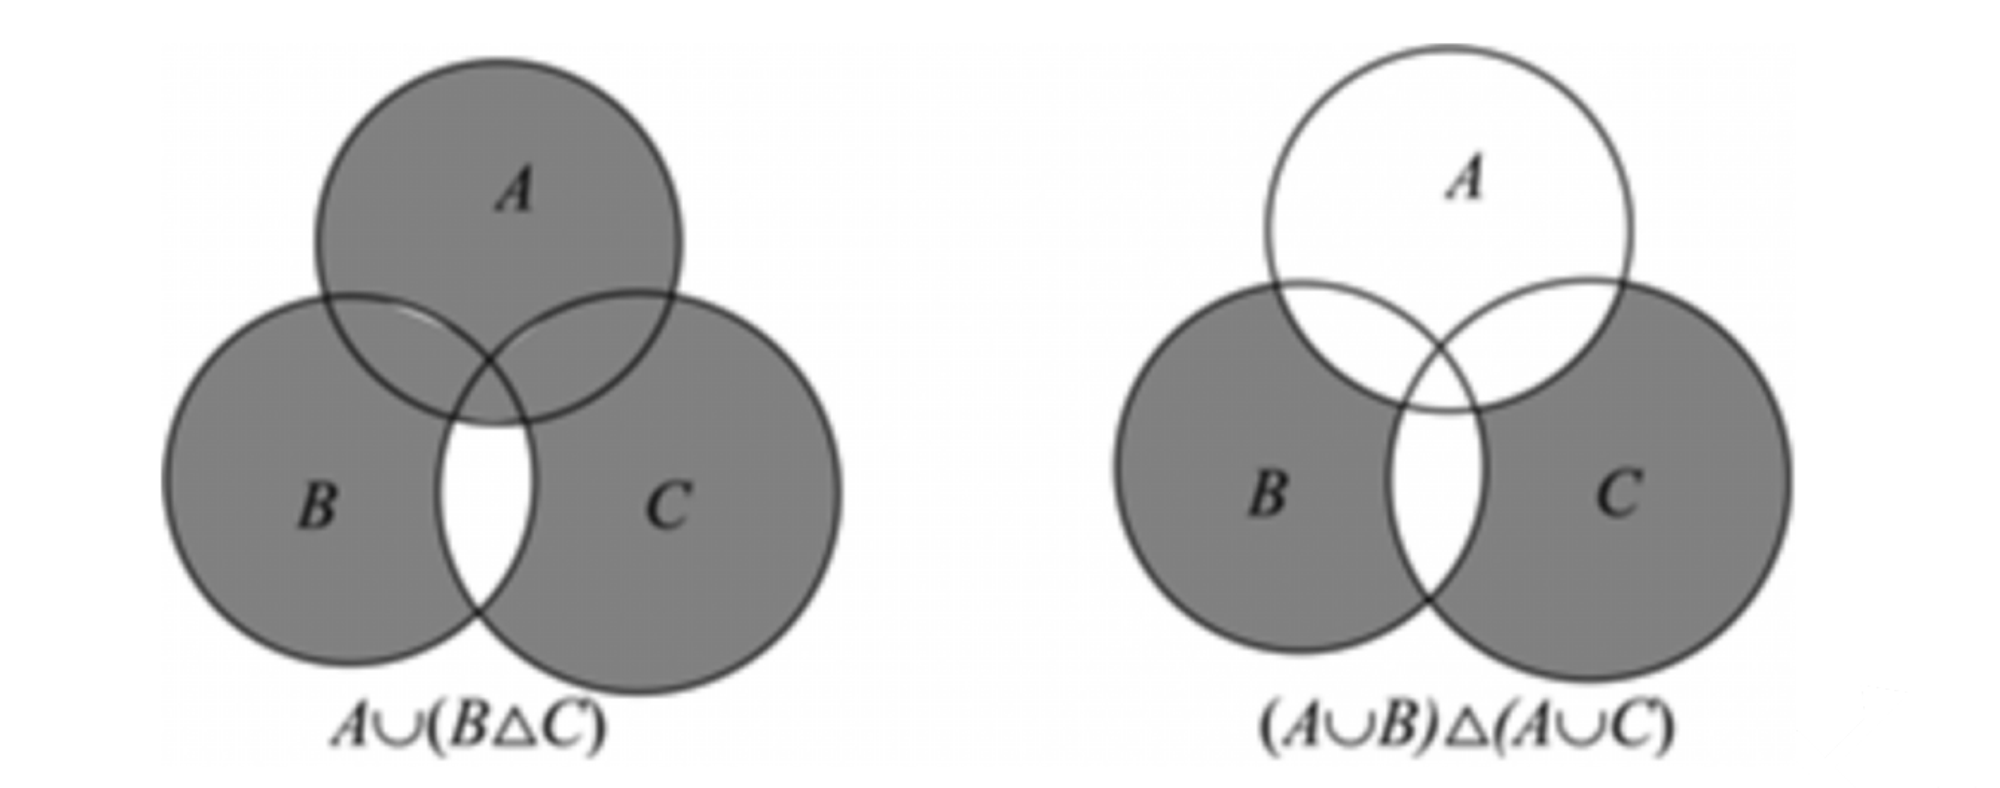
\includegraphics[width=0.85\textwidth]{figures/gao115_q13.png}
\end{center}
\step{所以 $A\cup(B\triangle C)\neq(A\cup B)\triangle(A\cup C)$，④错.}
\step{故选 $C$.}
\solend
\fi

\item 设 $a$、$b$、$c$、$p$ 为实数，若同时满足不等式 $ax^2+bx+c>0$、$bx^2+cx+a>0$ 与 $cx^2+ax+b>0$ 的全体实数 $x$ 所组成的集合等于 $(p,+\infty)$，则关于结论：① $a$、$b$、$c$ 至少有一个为 $0$；② $p=0$. 下列判断中正确的是\mbox{（\quad）}

\keepwithprev
A. ①和②都正确\qquad B. ①和②都错误\qquad C. ①正确，②错误\qquad D. ①错误，②正确

\ifanswer
\solbegin
\step{若同时满足不等式 $ax^2+bx+c>0$、$bx^2+cx+a>0$ 与 $cx^2+ax+b>0$ 的}
\step{全体实数 $x$ 所组成的集合等于 $(p,+\infty)$，必有 $a$,$b$,$c\geqslant0$，}
\step{不妨假设 $a$、$b$、$c$ 没有一个为 $0$，}
\step{则三个不等式均为开口向上的二次函数大于 $0$ 的部分，}
\step{解集的交集应为 $(-\infty,m)\cup(n,+\infty)$ 的形式，矛盾，}
\step{所以 $a$、$b$、$c$ 至少有一个为 $0$，故①正确：}
\step{不妨设 $a=0$，则 $b$,$c\geqslant0$，则不等式组化为 $\begin{cases}bx+c>0\\bx^2+cx>0,\\cx^2+b>0\end{cases}$}
\step{所以 $\begin{cases}x>-\dfrac cb\\x<-\dfrac cb\text{或}x>0\\x\in\R\end{cases}$，取交集得 $(0,+\infty)$，故 $p=0$，故②正确：}
\step{故选 $A$.}
\solend
\fi

\end{enumerate}

\bigsec{三、解答题}

\begin{enumerate}
\setcounter{enumi}{14}

\item 已知 $a>0$，$b>0$，

（1）试比较 $\dfrac{a^2-b^2}{a^2+b^2}$ 与 $\dfrac{a-b}{a+b}$ 的大小；

（2）若 $a+b>4$，求证：$\dfrac a{b+2}$ 和 $\dfrac b{a+2}$ 中至少有一个大于 $\dfrac12$.

\ifanswer
\solbegin
\step{（1）已知 $a>0$，$b>0$，$\dfrac{a^2-b^2}{a^2+b^2}-\dfrac{a-b}{a+b}=\dfrac{2ab(a-b)}{(a^2+b^2)(a+b)}$，}
\step{当 $a>b$ 时，$a-b>0$，所以 $\dfrac{a^2-b^2}{a^2+b^2}-\dfrac{a-b}{a+b}>0$，所以 $\dfrac{a^2-b^2}{a^2+b^2}>\dfrac{a-b}{a+b}$；}
\step{当 $a=b$ 时，$a-b=0$，所以 $\dfrac{a^2-b^2}{a^2+b^2}-\dfrac{a-b}{a+b}=0$，所以 $\dfrac{a^2-b^2}{a^2+b^2}=\dfrac{a-b}{a+b}$；}
\step{当 $a<b$ 时，$a-b<0$，所以 $\dfrac{a^2-b^2}{a^2+b^2}-\dfrac{a-b}{a+b}<0$，所以 $\dfrac{a^2-b^2}{a^2+b^2}<\dfrac{a-b}{a+b}$；}
\step{（2）假设 $\dfrac a{b+2}$ 和 $\dfrac b{a+2}$ 中都不大于 $\dfrac12$，即 $\dfrac b{a+2}\leqslant\dfrac12$，$\dfrac a{b+2}\leqslant\dfrac12$，}
\step{因为 $a>0$，$b>0$，所以 $a+2>0$，$b+2>0$，}
\step{所以 $2b\leqslant a+2$，$2a\leqslant b+2$，}
\step{两式相加得 $2a+2b\leqslant a+2+b+2=a+b+4$，即 $a+b\leqslant4$，}
\step{与已知 $a+b>4$ 矛盾，所以假设错误，}
\step{故 $\dfrac a{b+2}$ 和 $\dfrac b{a+2}$ 中至少有一个大于 $\dfrac12$.}
\solend
\fi

\item 某企业原有 $200$ 名科技人员，年人均工资 $a$ 万元($a>0$). 现加大对某芯片研发力度，该企业把原有 $200$ 名科技人员调整成技术人员和研发人员，其中技术人员 $x$ 名($x\in\N$ 且 $40\leqslant x\leqslant80$). 调整后，研发人员的年人均工资比调整前增加了 $(2x)\%$，技术人员的年人均工资为 $a\left(m-\dfrac x{10}\right)$万元.

（1）若要使调整后研发人员的年总工资不低于调整前 $200$ 名科技人员年总工资的 $1.5$ 倍，求调整后的技术人员最少有多少人？

（2）为了激励研发人员的工作热情和保持技术人员的工作积极性，企业决定在工资方面要同时满足以下两个条件：

①研发人员的年总工资始终不低于技术人员的年总工资；

②技术人员的年人均工资始终不低于调整前 $200$ 名科技人员的年人均工资.

请问是否存在这样的实数 $m$？若存在，求出 $m$ 的范围；若不存在，说明理由.

\ifanswer
\solbegin
\step{（1）由题意得调整后研发人员的年人均工资为 $[1+(2x)\%]a$ 万元，}
\step{那么 $(200-x)[1+(2x)\%]a\geqslant1.5\times200a$ ($a>0$)，}
\step{化简得 $x^2-150x+5000\leqslant0$，解得 $50\leqslant x\leqslant100$，}
\step{由于 $x\in\N$ 且 $40\leqslant x\leqslant80$，因此 $50\leqslant x\leqslant80$，}
\step{因此调整后的技术人员的人数最少为 $50$ 人；}
\step{（2）假设存在实数 $m$，使得技术人员在已知范围内调整后，满足以上两个条件，}
\step{由条件①得 $(200-x)[1+(2x)\%]a\geqslant x\left(m-\dfrac x{10}\right)a$，}
\step{整理得 $m\leqslant\dfrac{200}{x}+\dfrac{2x}{25}+3$；}
\step{因为 $\dfrac{200}{x}+\dfrac{2x}{25}+3\geqslant2\sqrt{\dfrac{200}{x}\cdot\dfrac{2x}{25}}+3=11$，}
\step{当且仅当 $\dfrac{200}{x}=\dfrac{2x}{25}$，即 $x=50$ 时取等号，因此 $m\leqslant11$，}
\step{由条件②得 $a\left(m-\dfrac x{10}\right)\geqslant a$，所以 $m\geqslant\dfrac x{10}+1$；}
\step{又由于 $40\leqslant x\leqslant80$，因此 $m\geqslant9$.}
\step{因此 $m\in[9,11]$.}
\solend
\fi

\item 已知 $a\in\R$，记 $f(x)=ax^2-(a+2)x+2$.

（1）若 $f(x)<3-2x$ 对于一切 $x\in\R$ 恒成立，求实数 $a$ 的取值范围；

（2）求关于 $x$ 不等式 $f(x)\geqslant0$ 的解集；

（3）若存在 $m\in\R$ 使关于 $x$ 的方程 $ax^2-(a+2)\lvert x\rvert+2=\lvert m+2\rvert+\lvert m-1\rvert$ 有四个不同的实根，求实数 $a$ 的取值范围.

\ifanswer
\solbegin
\step{（1）由 $f(x)<3-2x$ 对于一切 $x\in\R$ 恒成立，}
\step{得 $ax^2-ax-1<0$ 对于一切 $x\in\R$ 恒成立，}
\step{当 $a=0$ 时，原式可化为 $-1<0$，恒成立，符合条件；}
\step{当 $a\neq0$ 时，需满足 $\begin{cases}a<0\\\Delta=a^2+4a<0\end{cases}$，解得 $-4<a<0$；}
\step{综上，实数 $a$ 的取值范围是 $(-4,0]$；}
\step{（2）$f(x)\geqslant0$，即 $(ax-2)(x-1)\geqslant0$，}
\step{当 $a=0$ 时，原式化为 $-2x+2\geqslant0$，解集为 $\{x\mid x\leqslant1\}$；}
\step{当 $a>0$ 时，若 $a=2$，原式化为 $2(x-1)^2\geqslant0$，解集为 $\R$；}
\step{若 $0<a<2$，$\dfrac2a>1$，解集为 $\{x\mid x\leqslant1$ 或 $x\geqslant\dfrac2a\}$；}
\step{若 $a>2$，$\dfrac2a<1$，解集为 $\{x\mid x\leqslant\dfrac2a$ 或 $x\geqslant1\}$；}
\step{当 $a<0$ 时，$\dfrac2a<1$，解集为 $\left\{x\,\middle\vert\,\dfrac2a\leqslant x\leqslant1\right\}$；}
\step{综上，当 $a<0$ 时，不等式解集为 $\left\{x\,\middle\vert\,\dfrac2a\leqslant x\leqslant1\right\}$；}
\step{当 $a=0$ 时，不等式解集为 $\{x\mid x\leqslant1\}$；}
\step{当 $0<a<2$ 时，不等式解集为 $\{x\mid x\leqslant1$ 或 $x\geqslant\dfrac2a\}$；}
\step{当 $a=2$ 时，不等式解集为 $\R$；}
\step{当 $a>2$ 时，不等式解集为 $\{x\mid x\leqslant\dfrac2a$ 或 $x\geqslant1\}$；}
\step{（3）由绝对值三角不等式得 $\lvert m+2\rvert+\lvert m-1\rvert\geqslant\lvert(m+2)-(m-1)\rvert=3$，}
\step{即右侧取值范围为 $[3,+\infty)$，}
\step{令 $t=\lvert x\rvert\geqslant0$，原方程转化为 $at^2-(a+2)t+2=k$，$k\in[3,+\infty)$，}
\step{若原方程有四个不同实根，}
\step{需存在 $k\geqslant3$，使得方程 $at^2-(a+2)t+2-k=0$ 有两个不同正实根，}
\step{当 $a\geqslant0$ 时，方程的两根之积为 $\dfrac{2-k}{a}$，}
\step{因为 $k\geqslant3$，所以 $2-k\leqslant-1<0$，两根一正一负，}
\step{最多只有一个正根，对应最多两个 $x$ 根，不符合要求；}
\step{当 $a<0$ 时，两根之积为正，}
\step{要两个根都为正，需要两根之和 $\dfrac{a+2}{a}>0$，解得 $a<-2$，}
\step{再要求存在 $k\geqslant3$ 使得判别式大于 $0$，}
\step{即 $\triangle=(a+2)^2-4a(2-k)>0$ 在 $k\in[3,+\infty)$ 上有解，}
\step{即 $(a-2)^2+4ak>0$ 在 $k\in[3,+\infty)$ 上有解，}
\step{由 $a<0$，得 $(a-2)^2+12a>0$，}
\step{即 $a^2+8a+4>0$，结合 $a<-2$ 解得 $a<-4-2\sqrt3$，}
\step{故实数 $a$ 的取值范围是 $(-\infty,-4-2\sqrt3)$.}
\solend
\fi

\item 设 $A=\{x_1,x_2,\cdots,x_n\}(n\geqslant2,n\in\N)$，且 $x_1,x_2,\cdots,x_n$ 均为正整数，若对于 $A$ 中任意两个元素 $a,b$，当 $a>b$ 时，都有 $\dfrac{b^2}{a-b}\in A$，则称 $A$ 为“$n$ 元好集”.

（1）判断 $\{2,4,6\}$ 是否为“三元好集”，并说明理由；

（2）若集合 $M$ 为“二元好集”，且 $M$ 中所有元素之积小于 $2026$，求所有满足条件的集合 $M$ 的个数；

（3）设 $k\geqslant3,k\in\N$，是否存在“$k$ 元好集”，若存在，求出所有满足条件的“$k$ 元好集”，若不存在，请说明理由.

\ifanswer
\solbegin
\step{（1）取 $a=6,b=2$，则 $\dfrac{b^2}{a-b}=\dfrac44=1\notin\{2,4,6\}$，所以该集合不是三元好集.}
\step{（2）设 $M=\{b,a\}$，其中 $a>b$ 且均为正整数，则 $\dfrac{b^2}{a-b}$ 等于 $a$ 或 $b$.}
\step{若 $\dfrac{b^2}{a-b}=a$，则 $a^2-ab-b^2=0$，从而 $\dfrac ab=\dfrac{1+\sqrt5}{2}$，与 $\dfrac ab$ 为有理数矛盾.}
\step{若 $\dfrac{b^2}{a-b}=b$，则 $a=2b$；}
\step{反之，任意正整数 $b$ 对应的 $\{b,2b\}$ 均为二元好集.}
\step{由元素之积小于 $2026$，得 $2b^2<2026\Leftrightarrow b^2<1013$.}
\step{因为 $31^2=961<1013<1024=32^2$，所以 $b=1,2,\cdots,31$，}
\step{对应 $31$ 个不同的集合.}
\step{（3）假设存在 $k\geqslant3$ 的 $k$ 元好集 $A$，将其元素从小到大排列，}
\step{记最小元素为 $u$，次小元素为 $v$，最大元素为 $w$，则 $0<u<v<w$.}
\step{由 $\dfrac{u^2}{w-u}\in A$，该数不小于 $u$，得 $\dfrac{u^2}{w-u}\geqslant u\Rightarrow w\leqslant2u$.}
\step{又由 $\dfrac{u^2}{v-u}$,$\dfrac{v^2}{w-v}\in A$，这两个数均不超过 $w$，}
\step{得 $\dfrac{u^2}{v-u}\leqslant w$,$\dfrac{v^2}{w-v}\leqslant w$，}
\step{分母均为正，分别去分母后相加，}
\step{得 $u^2+v^2\leqslant w(v-u)+w(w-v)=w(w-u)\leqslant2u^2$，}
\step{于是 $v^2\leqslant u^2$，与 $v>u>0$ 矛盾，所以不存在 $k\geqslant3$ 的 $k$ 元好集.}
\solend
\fi

\end{enumerate}

\end{document}
"
%
% 原始材料：微信公众号“魔都数学加油站”文章，作者破晓，2026-11-06 17:58 发布；
% 连载“27学年高一115”，原文标题“27学年高一115——2026-2027年上海市复旦附中高一上10月阶段练习”；
% 原文链接：https://mp.weixin.qq.com/s/krocP0fMQQ4VM1SQEcLI2Q。
% 正文为 12 张 PNG 页（第 4、6、12 页 2560×3620，其余 4762×6735），
% 题目下印有【解析】或【答案】，为讲评版。
% 题目、解析均据原图转录；卷面红色水印及公众号页脚未录入。
%
% 卷首标题：原卷印作“2026-2027 年复旦附中高一上 10 月阶段练习”（公众号标题中的“上海市”
% 卷面标题行没有，本稿照卷面），年份区间按全稿惯例排 en dash；原卷未印副标题，本稿按题目内容
% 标为“集合与常用逻辑用语、不等式”。
%
% 与原卷的排版差异：
%   ① 原文从第 3 题起，填空题编号为 3—10、选择题为 11—14、解答题为 15—18，共 16 题，
%      本稿保留原题号（与多数卷的 3—21 不同）；
%   ② 原卷每题下直接印【解析】／【答案】，本稿按全稿惯例置于答案版；第 11 题把答案“$B$”
%      印在题干括号内且无【解析】，另提 \ans{}；其余选择题答案在解析末句“故选 …”，括号内留空；
%   ③ 原卷未印副标题，本稿按“知识模块”口径补出；
%   ④ 原卷填空横线按全稿惯例排为 \blankline[4.4em]；选择题括号排 \mbox{（\quad）}、
%      选项段前按惯例加 \keepwithprev；解答题不留作答区（原卷为讲评版，与 109—114 同）；
%   ⑤ 原卷数集排斜体 $R$／$Q$／$N$，按全稿惯例改 \R、\Q、\N。
%
% 判别式与对称差字形：原卷 $\triangle$（等边、扁）与 $\Delta$（等腰、高）两种混用，逐处照录——
%   第 7 题与第 17 题 (3) 的判别式、第 13 题的对称差 $A\triangle B$ 用 \triangle，
%   第 17 题 (1) cases 的判别式用 \Delta。
%
% 子集符号：第 4 题解析的 $(-1,3)\subset(-m,m)$ 印单线（真子集、无下划线），按 18／96
%   成例照录 \subset；第 5 题解析的 $B\subseteq A$ 印有下划线，照录 \subseteq。
%   第 3 题的补集照原卷上划线排 \overline{N}。
%
% 原卷存疑照录：第 9 题解析末行“故可能成立的是①②③”与四种情形的编号一致，照录；
%   第 10 题解析两幅函数图上另有蓝色／红色手写标注（$t$、$t+1$、$s$、$\frac16$ 等），
%   系批改笔迹，随裁图保留、不另作正文录入；第 14 题解析的 cases 三行照原卷排；
%   第 18 题 (2) 解析“所以该集合不是三元好集”前的取例 $a=6,b=2$ 照录。
%
% 行数核对：逐题数 \step/\stepm 条数，合计 133 条（Q3：3；Q4：3；Q5：4；Q6：5；Q7：4；
% Q8：4；Q9：11；Q10：7；Q11：0；Q12：4；Q13：8；Q14：9；Q15：10；Q16：13；
% Q17：32；Q18：16），与原卷印刷行逐题相等（cases 块作一个印刷行计）。第 11 题括号内印
% 答案且无解析，提 \ans{}，不计入 \step 账；第 10、13 题解析内的插图不计入 \step 账。
%
\documentclass[a4paper,11pt]{article}
\usepackage{common}

\begin{document}

\examtitlest[3]{2026--2027 年复旦附中高一上 10 月阶段练习}{集合与常用逻辑用语、不等式}

\bigsec{一、填空题}

\begin{enumerate}
\setcounter{enumi}{2}

\item 已知集合 $M=\{x\mid 4x^2-4x-15>0\}$，$N=\left\{x\,\middle\vert\,\dfrac{x+1}{x-6}>0\right\}$，则 $M\cap\overline{N}=$\blankline[4.4em].

\ifanswer
\solbegin
\step{集合 $M=\{x\mid 4x^2-4x-15>0\}=\{x\mid x>\dfrac52$ 或 $x<-\dfrac32\}$，}
\step{$N=\left\{x\,\middle\vert\,\dfrac{x+1}{x-6}>0\right\}=\{x\mid x>6$ 或 $x<-1\}$，得 $\overline{N}=\{x\mid-1\leqslant x\leqslant6\}$，}
\step{故 $M\cap\overline{N}=\left\{x\,\middle\vert\,\dfrac52<x\leqslant6\right\}$.}
\solend
\fi

\item 已知 $m>0$，不等式 $\lvert x\rvert<m$ 成立的一个充分不必要条件是 $-1<x<3$，则 $m$ 的取值范围是\blankline[4.4em].

\ifanswer
\solbegin
\step{不等式 $-m<x<m$ 成立的一个充分不必要条件是 $-1<x<3$，}
\step{由题意得 $(-1,3)\subset(-m,m)$，则 $m\geqslant3$，此时 $-m\leqslant-3<-1$，}% 原卷印单线 \subset，照录
\step{所以 $m$ 的取值范围是 $\{m\mid m\geqslant3\}$.}
\solend
\fi

\item 已知集合 $A=\{1,2\}$，集合 $B=\{x\mid ax=6\}$，若 $A\cup B=A$，则 $a$ 的所有取值构成的集合为\blankline[4.4em].

\ifanswer
\solbegin
\step{因为 $A\cup B=A$，所以 $B\subseteq A$，}
\step{当 $a=0$ 时，$B=\varnothing$，满足 $B\subseteq A$；}
\step{当 $a\neq0$ 时，$B=\left\{\dfrac6a\right\}$，则 $\dfrac6a=1$ 或 $\dfrac6a=2$，解得 $a=6$ 或 $a=3$，}
\step{综上所述，$a$ 的所有取值构成的集合为 $\{0,3,6\}$.}
\solend
\fi

\item 若关于 $x$ 的不等式 $ax^2+bx+c>0$ 的解集为 $(-3,2)$，则不等式 $ax^2+(a+b)x+c-2a>0$ 的解集为\blankline[4.4em].

\ifanswer
\solbegin
\step{由 $ax^2+bx+c>0$ 的解集为 $(-3,2)$ 得 $a<0$，}
\step{且 $ax^2+bx+c=0$ 时 $x_1=-3$，$x_2=2$，}
\step{得 $-3+2=-\dfrac ba$，即 $b=a$，$-3\times2=\dfrac ca$，即 $c=-6a$，}
\step{代入 $ax^2+(a+b)x+c-2a>0$ 得 $ax^2+2ax-8a>0$ 化简得 $x^2+2x-8<0$，}
\step{解得 $-4<x<2$，故解集为 $(-4,2)$.}
\solend
\fi

\item 已知关于 $x$ 的方程 $x^2-2x+m=0$ 的两个实数根分别为 $x_1$，$x_2$. 若 $x_1^2x_2^2+x_1^2+x_2^2=7$，则实数 $m$ 的值为\blankline[4.4em].

\ifanswer
\solbegin
\step{由韦达定理得 $x_1+x_2=2$，$x_1x_2=m$，}
\step{$x_1^2x_2^2+x_1^2+x_2^2=(x_1x_2)^2+(x_1+x_2)^2-2x_1x_2=m^2+4-2m$，}
\step{由 $m^2+4-2m=7$，得 $m^2-2m-3=0$，解得 $m=3$ 或 $m=-1$，}
\step{方程有两个实数根，故 $\triangle=4-4m\geqslant0$，即 $m\leqslant1$，所以 $m=-1$.}
\solend
\fi

\item 已知 $x>1$，若 $x^2-xy+y=0$，则 $x+y$ 的最小值是\blankline[4.4em].

\ifanswer
\solbegin
\step{由于 $x^2-xy+y=0$，则 $y=\dfrac{x^2}{x-1}>0$，}
\step{则 $x+y=x+\dfrac{x^2}{x-1}=\dfrac{2x^2-x}{x-1}=\dfrac{2(x-1)^2+3(x-1)+1}{x-1}$}
\step{$=2(x-1)+\dfrac1{x-1}+3\geqslant2\sqrt{2(x-1)\cdot\dfrac1{x-1}}+3=2\sqrt2+3$，}
\step{当且仅当 $x=1+\dfrac{\sqrt2}{2}$ 时取等号，故最小值是 $2\sqrt2+3$.}
\solend
\fi

\item 若集合 $A=B_1\cup B_2\cup\cdots\cup B_n$，其中 $B_1$、$B_2$、$\cdots$、$B_n$ 为非空集合，$B_i\cap B_j=\varnothing$，$1\leqslant i<j\leqslant n$，则称集合 $\{B_1,B_2,\cdots,B_n\}$ 为集合 $A$ 的一个 $n$ 划分. 例如：集合 $\{\{1,2\},\{3\}\}$，$\{\{1,3\},\{2\}\}$，$\{\{2,3\},\{1\}\}$ 均为集合 $\{1,2,3\}$ 的一个 $2$ 划分. 设 $\{B_1,B_2\}$ 为有理数集 $\Q$ 的一个 $2$ 划分，且满足对任意 $x\in B_1$，任意 $y\in B_2$，都有 $x<y$. 则对于 $B_1$、$B_2$ 有：

① $B_1$ 中的元素存在最大值，$B_2$ 中的元素不存在最小值；

② $B_1$ 中的元素不存在最大值，$B_2$ 中的元素存在最小值；

③ $B_1$ 中的元素不存在最大值，$B_2$ 中的元素不存在最小值；

④ $B_1$ 中的元素存在最大值，$B_2$ 中的元素存在最小值；

对于以上四种情况，可能成立的序号有\blankline[4.4em].

\ifanswer
\solbegin
\step{对于①，$B_1=\{x\in\Q\mid x\leqslant2\}$，$B_2=\{x\in\Q\mid x>2\}$，①可能成立；}
\step{对于②，$B_1=\{x\in\Q\mid x<2\}$，$B_2=\{x\in\Q\mid x\geqslant2\}$，②可能成立；}
\step{对于③，$B_1=\{x\in\Q\mid x<\pi\}$，$B_2=\{x\in\Q\mid x>\pi\}$，③可能成立；}
\step{对于④，假设④成立，}
\step{不妨设 $B_1$ 中的元素的最大值为 $s$，$B_2$ 中的元素的最小值为 $t$，}
\step{由题意得 $s<t$，所以 $s<\dfrac{s+t}{2}<t$，}
\step{因为 $s$ 为 $B_1$ 中的元素的最大值，所以 $\dfrac{s+t}{2}\notin B_1$，}
\step{因为 $t$ 为 $B_2$ 中的元素的最小值，所以 $\dfrac{s+t}{2}\notin B_2$，}
\step{又 $B_1\cup B_2=\Q$，所以 $\dfrac{s+t}{2}\notin\Q$，与 $\dfrac{s+t}{2}\in\Q$ 矛盾，}
\step{所以假设不成立，即④不可能成立.}
\step{故可能成立的是①②③.}
\solend
\fi

\item 已知集合 $A=\left[s,s+\dfrac16\right]\cup[t,t+1]$，其中 $1\notin A$ 且 $s+\dfrac16<t$，函数 $f(x)=\dfrac x{x-1}$，且对任意 $a\in A$，都有 $f(a)\in A$，则 $t$ 的值是\blankline[4.4em].

\ifanswer
\solbegin
\step{若 $\left[s,s+\dfrac16\right]$,$[t,t+1]$ 在 $f(x)=\dfrac x{x-1}$ 图像的同侧，}
\step{则点 $\left(t,s+\dfrac16\right)$,$(t+1,s)$ 在 $f(x)=\dfrac x{x-1}$ 的图像上，}
\step{所以 $\dfrac t{t-1}=\dfrac{t+1}{t}+\dfrac16$，解得 $t=-2$ 或 $t=3$，检验得 $t=3$；}
\step{若 $\left[s,s+\dfrac16\right]$,$[t,t+1]$ 在 $f(x)=\dfrac x{x-1}$ 图像的两侧，}
\step{则点 $(t,t+1)$ 在 $f(x)=\dfrac x{x-1}$ 的图像上，}
\step{所以 $t+1=\dfrac t{t-1}$，解得 $t=\dfrac{1\pm\sqrt5}{2}$，检验得 $t=\dfrac{1+\sqrt5}{2}$，}
\step{综上，$t=\dfrac{1+\sqrt5}{2}$ 或 $t=3$.}
\begin{center}
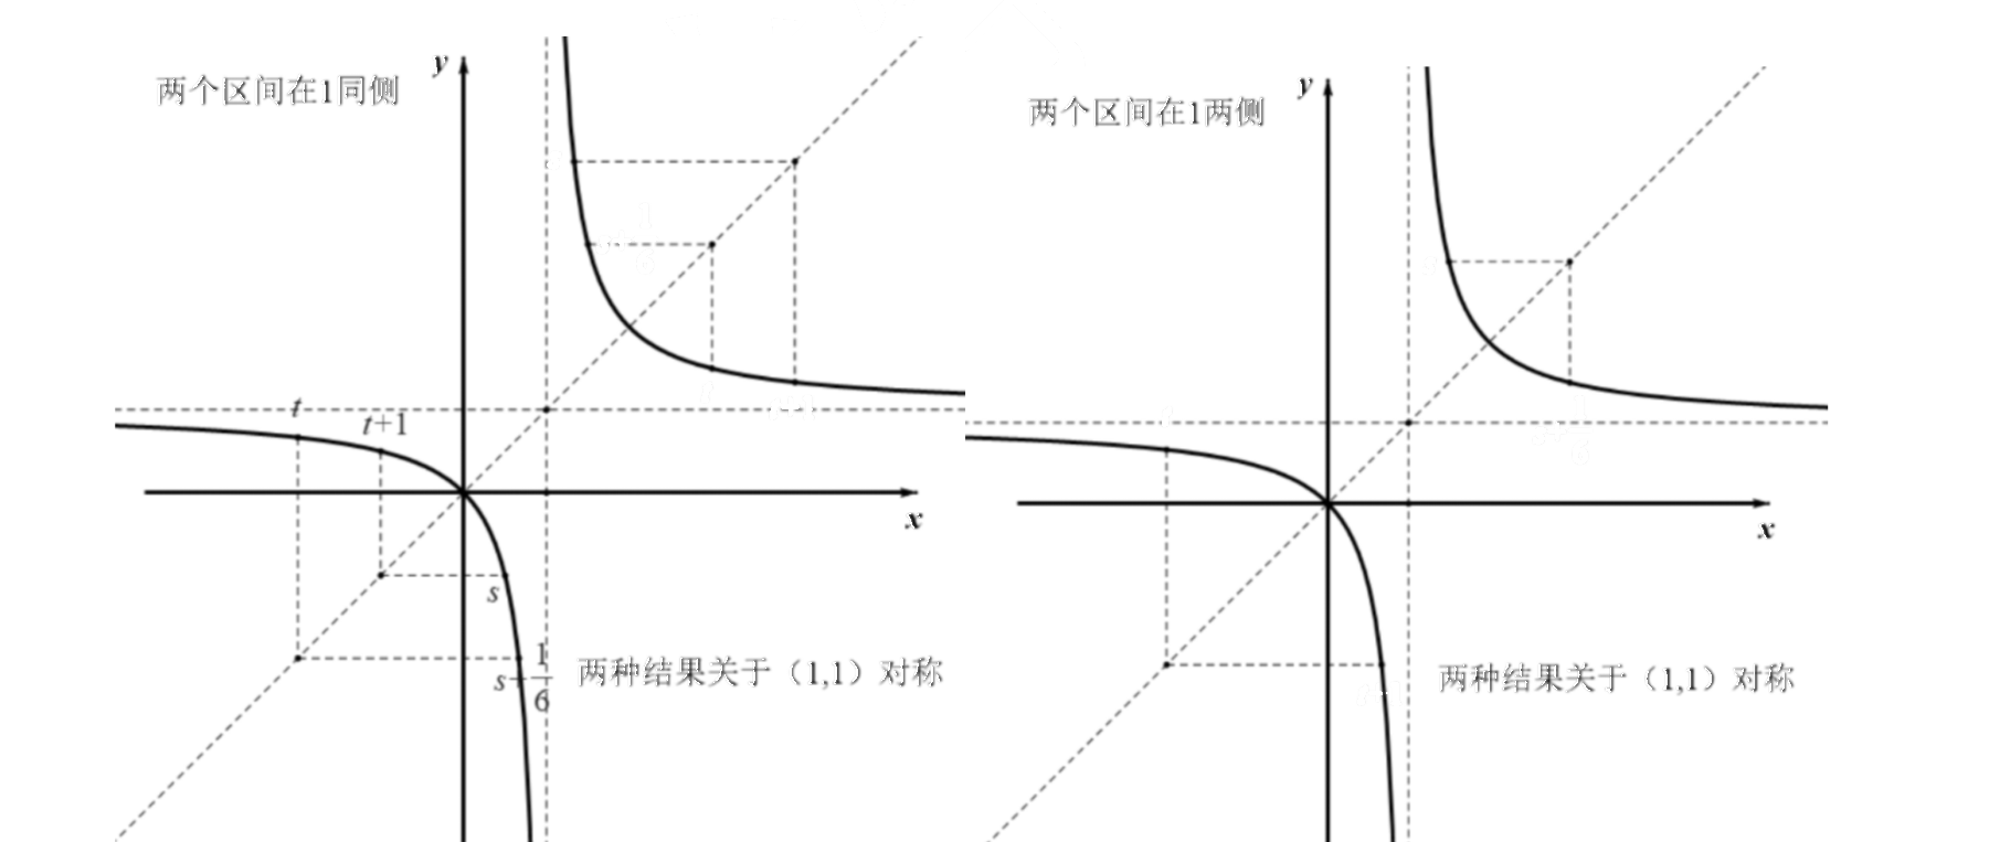
\includegraphics[width=0.92\textwidth]{figures/gao115_q10.png}
\end{center}
\solend
\fi

\end{enumerate}

\bigsec{二、选择题}

\begin{enumerate}
\setcounter{enumi}{10}

\item “对任意有理数 $x$ 都有 $x^2\neq2$”的否定形式是\mbox{（\quad）}% 原卷把答案“$B$”印在题干括号内、无【解析】

\keepwithprev
A. 存在有理数 $x$ 使得 $x^2\neq2$\qquad\qquad B. 存在有理数 $x$ 使得 $x^2=2$

C. 存在无理数 $x$ 使得 $x^2\neq2$\qquad\qquad D. 存在无理数 $x$ 使得 $x^2=2$

\ifanswer
\ans{$B$}
\fi

\item 已知 $a$、$b$ 都是实数，那么“$a^3>b^3$”是“$a^2>b^2$”的\mbox{（\quad）}

\keepwithprev
A. 充分不必要条件\qquad\qquad B. 必要不充分条件

C. 充要条件\qquad\qquad\qquad D. 既不充分也不必要条件

\ifanswer
\solbegin
\step{因为 $a^3>b^3$ 等价于 $a>b$，}
\step{由于 $a$、$b$ 正负不定，所以由 $a>b$ 不能得到 $a^2>b^2$，}
\step{由 $a^2>b^2$ 也不能得到 $a>b$，}
\step{因此“$a^3>b^3$”是“$a^2>b^2$”的既不充分也不必要条件. 故选 $D$.}
\solend
\fi

\item 定义集合运算 $A-B=\{x\mid x\in A$ 且 $x\notin B\}$，将 $A\triangle B=(A-B)\cup(B-A)$ 称为集合 $A$ 与集合 $B$ 的对称差.

命题一：$A\triangle B=B\triangle A$；

命题二：$A\triangle\varnothing=A$；

命题三：$A\cap(B\triangle C)=(A\cap B)\triangle(A\cap C)$；

命题四：$A\cup(B\triangle C)=(A\cup B)\triangle(A\cup C)$；

其中正确命题的个数是\mbox{（\quad）}

\keepwithprev
A. $1$\qquad\qquad B. $2$\qquad\qquad C. $3$\qquad\qquad D. $4$

\ifanswer
\solbegin
\step{对于①，$B\triangle A=(B-A)\cup(A-B)=(A-B)\cup(B-A)=A\triangle B$，①对；}
\step{对于②，$A-B=\{x\mid x\in A$ 且 $x\notin B\}=\{x\mid x\in A$ 且 $x\notin(A\cap B)\}$}
\step{$=A-(A\cap B)$，则 $A\triangle\varnothing=(A-\varnothing)\cup(\varnothing-A)=A\cup\varnothing=A$，②对；}
\step{对于③，$A\cap(B\triangle C)=A\cap(B\cup C-B\cap C)=A\cap(B\cup C)-A\cap(B\cap C)$}
\step{$=(A\cap B)\cup(A\cap C)-(A\cap B)\cap(A\cap C)=(A\cap B)\triangle(A\cap C)$，③对；}
\step{对于④，如图所示：}
\begin{center}
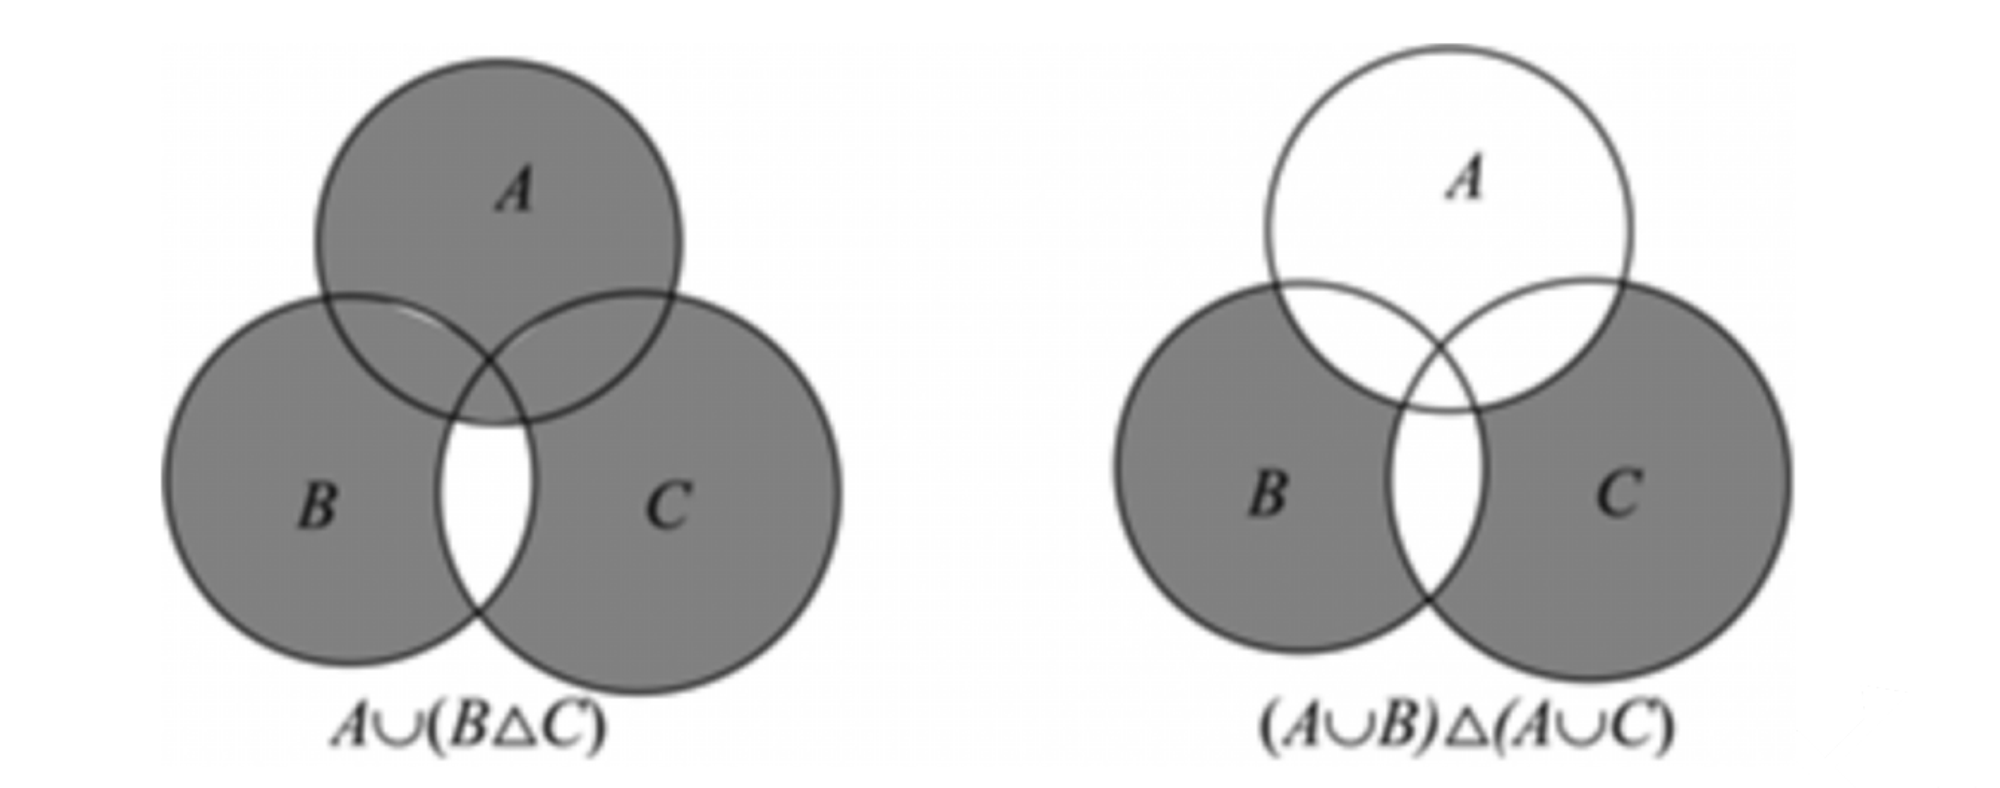
\includegraphics[width=0.85\textwidth]{figures/gao115_q13.png}
\end{center}
\step{所以 $A\cup(B\triangle C)\neq(A\cup B)\triangle(A\cup C)$，④错.}
\step{故选 $C$.}
\solend
\fi

\item 设 $a$、$b$、$c$、$p$ 为实数，若同时满足不等式 $ax^2+bx+c>0$、$bx^2+cx+a>0$ 与 $cx^2+ax+b>0$ 的全体实数 $x$ 所组成的集合等于 $(p,+\infty)$，则关于结论：① $a$、$b$、$c$ 至少有一个为 $0$；② $p=0$. 下列判断中正确的是\mbox{（\quad）}

\keepwithprev
A. ①和②都正确\qquad B. ①和②都错误\qquad C. ①正确，②错误\qquad D. ①错误，②正确

\ifanswer
\solbegin
\step{若同时满足不等式 $ax^2+bx+c>0$、$bx^2+cx+a>0$ 与 $cx^2+ax+b>0$ 的}
\step{全体实数 $x$ 所组成的集合等于 $(p,+\infty)$，必有 $a$,$b$,$c\geqslant0$，}
\step{不妨假设 $a$、$b$、$c$ 没有一个为 $0$，}
\step{则三个不等式均为开口向上的二次函数大于 $0$ 的部分，}
\step{解集的交集应为 $(-\infty,m)\cup(n,+\infty)$ 的形式，矛盾，}
\step{所以 $a$、$b$、$c$ 至少有一个为 $0$，故①正确：}
\step{不妨设 $a=0$，则 $b$,$c\geqslant0$，则不等式组化为 $\begin{cases}bx+c>0\\bx^2+cx>0,\\cx^2+b>0\end{cases}$}
\step{所以 $\begin{cases}x>-\dfrac cb\\x<-\dfrac cb\text{或}x>0\\x\in\R\end{cases}$，取交集得 $(0,+\infty)$，故 $p=0$，故②正确：}
\step{故选 $A$.}
\solend
\fi

\end{enumerate}

\bigsec{三、解答题}

\begin{enumerate}
\setcounter{enumi}{14}

\item 已知 $a>0$，$b>0$，

（1）试比较 $\dfrac{a^2-b^2}{a^2+b^2}$ 与 $\dfrac{a-b}{a+b}$ 的大小；

（2）若 $a+b>4$，求证：$\dfrac a{b+2}$ 和 $\dfrac b{a+2}$ 中至少有一个大于 $\dfrac12$.

\ifanswer
\solbegin
\step{（1）已知 $a>0$，$b>0$，$\dfrac{a^2-b^2}{a^2+b^2}-\dfrac{a-b}{a+b}=\dfrac{2ab(a-b)}{(a^2+b^2)(a+b)}$，}
\step{当 $a>b$ 时，$a-b>0$，所以 $\dfrac{a^2-b^2}{a^2+b^2}-\dfrac{a-b}{a+b}>0$，所以 $\dfrac{a^2-b^2}{a^2+b^2}>\dfrac{a-b}{a+b}$；}
\step{当 $a=b$ 时，$a-b=0$，所以 $\dfrac{a^2-b^2}{a^2+b^2}-\dfrac{a-b}{a+b}=0$，所以 $\dfrac{a^2-b^2}{a^2+b^2}=\dfrac{a-b}{a+b}$；}
\step{当 $a<b$ 时，$a-b<0$，所以 $\dfrac{a^2-b^2}{a^2+b^2}-\dfrac{a-b}{a+b}<0$，所以 $\dfrac{a^2-b^2}{a^2+b^2}<\dfrac{a-b}{a+b}$；}
\step{（2）假设 $\dfrac a{b+2}$ 和 $\dfrac b{a+2}$ 中都不大于 $\dfrac12$，即 $\dfrac b{a+2}\leqslant\dfrac12$，$\dfrac a{b+2}\leqslant\dfrac12$，}
\step{因为 $a>0$，$b>0$，所以 $a+2>0$，$b+2>0$，}
\step{所以 $2b\leqslant a+2$，$2a\leqslant b+2$，}
\step{两式相加得 $2a+2b\leqslant a+2+b+2=a+b+4$，即 $a+b\leqslant4$，}
\step{与已知 $a+b>4$ 矛盾，所以假设错误，}
\step{故 $\dfrac a{b+2}$ 和 $\dfrac b{a+2}$ 中至少有一个大于 $\dfrac12$.}
\solend
\fi

\item 某企业原有 $200$ 名科技人员，年人均工资 $a$ 万元($a>0$). 现加大对某芯片研发力度，该企业把原有 $200$ 名科技人员调整成技术人员和研发人员，其中技术人员 $x$ 名($x\in\N$ 且 $40\leqslant x\leqslant80$). 调整后，研发人员的年人均工资比调整前增加了 $(2x)\%$，技术人员的年人均工资为 $a\left(m-\dfrac x{10}\right)$万元.

（1）若要使调整后研发人员的年总工资不低于调整前 $200$ 名科技人员年总工资的 $1.5$ 倍，求调整后的技术人员最少有多少人？

（2）为了激励研发人员的工作热情和保持技术人员的工作积极性，企业决定在工资方面要同时满足以下两个条件：

①研发人员的年总工资始终不低于技术人员的年总工资；

②技术人员的年人均工资始终不低于调整前 $200$ 名科技人员的年人均工资.

请问是否存在这样的实数 $m$？若存在，求出 $m$ 的范围；若不存在，说明理由.

\ifanswer
\solbegin
\step{（1）由题意得调整后研发人员的年人均工资为 $[1+(2x)\%]a$ 万元，}
\step{那么 $(200-x)[1+(2x)\%]a\geqslant1.5\times200a$ ($a>0$)，}
\step{化简得 $x^2-150x+5000\leqslant0$，解得 $50\leqslant x\leqslant100$，}
\step{由于 $x\in\N$ 且 $40\leqslant x\leqslant80$，因此 $50\leqslant x\leqslant80$，}
\step{因此调整后的技术人员的人数最少为 $50$ 人；}
\step{（2）假设存在实数 $m$，使得技术人员在已知范围内调整后，满足以上两个条件，}
\step{由条件①得 $(200-x)[1+(2x)\%]a\geqslant x\left(m-\dfrac x{10}\right)a$，}
\step{整理得 $m\leqslant\dfrac{200}{x}+\dfrac{2x}{25}+3$；}
\step{因为 $\dfrac{200}{x}+\dfrac{2x}{25}+3\geqslant2\sqrt{\dfrac{200}{x}\cdot\dfrac{2x}{25}}+3=11$，}
\step{当且仅当 $\dfrac{200}{x}=\dfrac{2x}{25}$，即 $x=50$ 时取等号，因此 $m\leqslant11$，}
\step{由条件②得 $a\left(m-\dfrac x{10}\right)\geqslant a$，所以 $m\geqslant\dfrac x{10}+1$；}
\step{又由于 $40\leqslant x\leqslant80$，因此 $m\geqslant9$.}
\step{因此 $m\in[9,11]$.}
\solend
\fi

\item 已知 $a\in\R$，记 $f(x)=ax^2-(a+2)x+2$.

（1）若 $f(x)<3-2x$ 对于一切 $x\in\R$ 恒成立，求实数 $a$ 的取值范围；

（2）求关于 $x$ 不等式 $f(x)\geqslant0$ 的解集；

（3）若存在 $m\in\R$ 使关于 $x$ 的方程 $ax^2-(a+2)\lvert x\rvert+2=\lvert m+2\rvert+\lvert m-1\rvert$ 有四个不同的实根，求实数 $a$ 的取值范围.

\ifanswer
\solbegin
\step{（1）由 $f(x)<3-2x$ 对于一切 $x\in\R$ 恒成立，}
\step{得 $ax^2-ax-1<0$ 对于一切 $x\in\R$ 恒成立，}
\step{当 $a=0$ 时，原式可化为 $-1<0$，恒成立，符合条件；}
\step{当 $a\neq0$ 时，需满足 $\begin{cases}a<0\\\Delta=a^2+4a<0\end{cases}$，解得 $-4<a<0$；}
\step{综上，实数 $a$ 的取值范围是 $(-4,0]$；}
\step{（2）$f(x)\geqslant0$，即 $(ax-2)(x-1)\geqslant0$，}
\step{当 $a=0$ 时，原式化为 $-2x+2\geqslant0$，解集为 $\{x\mid x\leqslant1\}$；}
\step{当 $a>0$ 时，若 $a=2$，原式化为 $2(x-1)^2\geqslant0$，解集为 $\R$；}
\step{若 $0<a<2$，$\dfrac2a>1$，解集为 $\{x\mid x\leqslant1$ 或 $x\geqslant\dfrac2a\}$；}
\step{若 $a>2$，$\dfrac2a<1$，解集为 $\{x\mid x\leqslant\dfrac2a$ 或 $x\geqslant1\}$；}
\step{当 $a<0$ 时，$\dfrac2a<1$，解集为 $\left\{x\,\middle\vert\,\dfrac2a\leqslant x\leqslant1\right\}$；}
\step{综上，当 $a<0$ 时，不等式解集为 $\left\{x\,\middle\vert\,\dfrac2a\leqslant x\leqslant1\right\}$；}
\step{当 $a=0$ 时，不等式解集为 $\{x\mid x\leqslant1\}$；}
\step{当 $0<a<2$ 时，不等式解集为 $\{x\mid x\leqslant1$ 或 $x\geqslant\dfrac2a\}$；}
\step{当 $a=2$ 时，不等式解集为 $\R$；}
\step{当 $a>2$ 时，不等式解集为 $\{x\mid x\leqslant\dfrac2a$ 或 $x\geqslant1\}$；}
\step{（3）由绝对值三角不等式得 $\lvert m+2\rvert+\lvert m-1\rvert\geqslant\lvert(m+2)-(m-1)\rvert=3$，}
\step{即右侧取值范围为 $[3,+\infty)$，}
\step{令 $t=\lvert x\rvert\geqslant0$，原方程转化为 $at^2-(a+2)t+2=k$，$k\in[3,+\infty)$，}
\step{若原方程有四个不同实根，}
\step{需存在 $k\geqslant3$，使得方程 $at^2-(a+2)t+2-k=0$ 有两个不同正实根，}
\step{当 $a\geqslant0$ 时，方程的两根之积为 $\dfrac{2-k}{a}$，}
\step{因为 $k\geqslant3$，所以 $2-k\leqslant-1<0$，两根一正一负，}
\step{最多只有一个正根，对应最多两个 $x$ 根，不符合要求；}
\step{当 $a<0$ 时，两根之积为正，}
\step{要两个根都为正，需要两根之和 $\dfrac{a+2}{a}>0$，解得 $a<-2$，}
\step{再要求存在 $k\geqslant3$ 使得判别式大于 $0$，}
\step{即 $\triangle=(a+2)^2-4a(2-k)>0$ 在 $k\in[3,+\infty)$ 上有解，}
\step{即 $(a-2)^2+4ak>0$ 在 $k\in[3,+\infty)$ 上有解，}
\step{由 $a<0$，得 $(a-2)^2+12a>0$，}
\step{即 $a^2+8a+4>0$，结合 $a<-2$ 解得 $a<-4-2\sqrt3$，}
\step{故实数 $a$ 的取值范围是 $(-\infty,-4-2\sqrt3)$.}
\solend
\fi

\item 设 $A=\{x_1,x_2,\cdots,x_n\}(n\geqslant2,n\in\N)$，且 $x_1,x_2,\cdots,x_n$ 均为正整数，若对于 $A$ 中任意两个元素 $a,b$，当 $a>b$ 时，都有 $\dfrac{b^2}{a-b}\in A$，则称 $A$ 为“$n$ 元好集”.

（1）判断 $\{2,4,6\}$ 是否为“三元好集”，并说明理由；

（2）若集合 $M$ 为“二元好集”，且 $M$ 中所有元素之积小于 $2026$，求所有满足条件的集合 $M$ 的个数；

（3）设 $k\geqslant3,k\in\N$，是否存在“$k$ 元好集”，若存在，求出所有满足条件的“$k$ 元好集”，若不存在，请说明理由.

\ifanswer
\solbegin
\step{（1）取 $a=6,b=2$，则 $\dfrac{b^2}{a-b}=\dfrac44=1\notin\{2,4,6\}$，所以该集合不是三元好集.}
\step{（2）设 $M=\{b,a\}$，其中 $a>b$ 且均为正整数，则 $\dfrac{b^2}{a-b}$ 等于 $a$ 或 $b$.}
\step{若 $\dfrac{b^2}{a-b}=a$，则 $a^2-ab-b^2=0$，从而 $\dfrac ab=\dfrac{1+\sqrt5}{2}$，与 $\dfrac ab$ 为有理数矛盾.}
\step{若 $\dfrac{b^2}{a-b}=b$，则 $a=2b$；}
\step{反之，任意正整数 $b$ 对应的 $\{b,2b\}$ 均为二元好集.}
\step{由元素之积小于 $2026$，得 $2b^2<2026\Leftrightarrow b^2<1013$.}
\step{因为 $31^2=961<1013<1024=32^2$，所以 $b=1,2,\cdots,31$，}
\step{对应 $31$ 个不同的集合.}
\step{（3）假设存在 $k\geqslant3$ 的 $k$ 元好集 $A$，将其元素从小到大排列，}
\step{记最小元素为 $u$，次小元素为 $v$，最大元素为 $w$，则 $0<u<v<w$.}
\step{由 $\dfrac{u^2}{w-u}\in A$，该数不小于 $u$，得 $\dfrac{u^2}{w-u}\geqslant u\Rightarrow w\leqslant2u$.}
\step{又由 $\dfrac{u^2}{v-u}$,$\dfrac{v^2}{w-v}\in A$，这两个数均不超过 $w$，}
\step{得 $\dfrac{u^2}{v-u}\leqslant w$,$\dfrac{v^2}{w-v}\leqslant w$，}
\step{分母均为正，分别去分母后相加，}
\step{得 $u^2+v^2\leqslant w(v-u)+w(w-v)=w(w-u)\leqslant2u^2$，}
\step{于是 $v^2\leqslant u^2$，与 $v>u>0$ 矛盾，所以不存在 $k\geqslant3$ 的 $k$ 元好集.}
\solend
\fi

\end{enumerate}

\end{document}
